% !TeX spellcheck = en_US
\documentclass{article}

% Pass options to natbib
\PassOptionsToPackage{numbers, compress}{natbib}

% NeurIPS packages
\usepackage[]{neurips_2023}
\usepackage[utf8]{inputenc} % allow utf-8 input
\usepackage[T1]{fontenc}    % use 8-bit T1 fonts
%\usepackage{hyperref}       % hyperlinks
\usepackage{url}            % simple URL typesetting
\usepackage{booktabs}       % professional-quality tables
\usepackage{amsfonts}       % blackboard math symbols
\usepackage{nicefrac}       % compact symbols for 1/2, etc.
\usepackage{microtype}      % microtypography
\usepackage{xcolor}         % colors

% Redefine paragraph to be tighter
\renewcommand{\paragraph}[1]{{\bf #1}~~}

% Array/table packages
\usepackage{tabularx}
\usepackage{array,multirow}
\usepackage{colortbl}
\newcommand{\PreserveBackslash}[1]{\let\temp=\\#1\let\\=\temp}
\newcolumntype{C}[1]{>{\PreserveBackslash\centering}p{#1}}
\newlength{\tblw}

% Latin
\usepackage{xspace}
\newcommand{\eg}{\textit{e.g.\@}\xspace}
\newcommand{\ie}{\textit{i.e.\@}\xspace}
\newcommand{\cf}{\textit{cf.\@}\xspace}
\newcommand{\etc}{\textit{etc.\@}\xspace}
\newcommand{\etal}{\textit{et~al.\@}\xspace}

% Our method
\newcommand{\our}{\textsc{sfr}\xspace}

% Tikz
\usepackage{tikz}
\usepackage{pgfplots}
\usetikzlibrary{patterns}
\usetikzlibrary{decorations,backgrounds,arrows.meta,calc}
\usetikzlibrary{shapes,arrows,positioning}

% Appendix/supplement title
\newcommand{\nipstitle}[1]{{%
    % rules for title box at top and bottom
    \def\toptitlebar{\hrule height4pt \vskip .25in \vskip -\parskip} 
    \def\bottomtitlebar{\vskip .29in \vskip -\parskip \hrule height1pt \vskip .09in} 
    \phantomsection\hsize\textwidth\linewidth\hsize%
    \vskip 0.1in%
    \toptitlebar%
    \begin{minipage}{\textwidth}%
        \centering{\LARGE\bf #1\par}%
    \end{minipage}%
    \bottomtitlebar%
    \addcontentsline{toc}{section}{#1}%
}}

% Bibliography
%\usepackage[maxcitenames=1, maxbibnames=4, doi=false, isbn=false, eprint=true, backend=bibtex, hyperref=true, url=false, style=authoryear-comp]{biblatex}
%\addbibresource{zotero-library.bib}
% \addbibresource{paper/zotero-library.bib}

% Let's use good old bibtex instead

% Figure customization: Tight legend box
\pgfplotsset{every axis/.append style={
		legend style={inner xsep=1pt, inner ysep=0.5pt, nodes={inner sep=1pt, text depth=0.1em},draw=none,fill=none}
}}

% Our packages
\usepackage{todonotes}
\usepackage[colorlinks=true,linkcolor=black,allcolors=black,urlcolor=black,citecolor=black]{hyperref}
\usepackage{amsmath}
\usepackage{bm}
\usepackage{algpseudocode}
\usepackage{algorithm}
\usepackage{derivative}
\usepackage{wrapfig}

\usepackage{tikz,pgfplots}
\usepackage{subcaption}
\usetikzlibrary{}

\input{aidans-utils.tex}

% Short section names etc
% This must be imported last!
%\usepackage{cleveref}
\usepackage[capitalise,nameinlink]{cleveref}
\crefname{section}{Sec.}{Secs.}
\crefname{algorithm}{Alg.}{Algs.}
\crefname{appendix}{App.}{Apps.}
\crefname{definition}{Def.}{Defs.}
\crefname{table}{Table}{Tables}

% Config for Arno's awesome TikZ plotting stuff
\newlength{\figurewidth}
\newlength{\figureheight}


% Variables
\newcommand{\state}{\ensuremath{\mathbf{s}}}
\newcommand{\action}{\ensuremath{\mathbf{a}}}
\newcommand{\noise}{\ensuremath{\bm\epsilon}}
\newcommand{\discount}{\ensuremath{\gamma}}
\newcommand{\inducingInput}{\ensuremath{\mathbf{Z}}}
\newcommand{\inducingVariable}{\ensuremath{\mathbf{u}}}
\newcommand{\dataset}{\ensuremath{\mathcal{D}}}
\newcommand{\dualParam}[1]{\ensuremath{\bm{\lambda}_{#1}}}
\newcommand{\meanParam}[1]{\ensuremath{\bm{\mu}_{#1}}}

% Indexes
\newcommand{\horizon}{\ensuremath{h}}
\newcommand{\Horizon}{\ensuremath{H}}
\newcommand{\numDataNew}{\ensuremath{N^{\text{new}}}}
\newcommand{\numDataOld}{\ensuremath{N^{\text{old}}}}
\newcommand{\numInducing}{\ensuremath{M}}

% Domains
\newcommand{\stateDomain}{\ensuremath{\mathcal{S}}}
\newcommand{\actionDomain}{\ensuremath{\mathcal{A}}}
\newcommand{\inputDomain}{\ensuremath{\mathbb{R}^{D}}}
\newcommand{\outputDomain}{\ensuremath{\mathbb{R}^{C}}}
\newcommand{\policyDomain}{\ensuremath{\Pi}}

% Functions
\newcommand{\rewardFn}{\ensuremath{r}}
\newcommand{\transitionFn}{\ensuremath{f}}
\newcommand{\latentFn}{\ensuremath{f}}

\newcommand{\optimisticTransition}{\ensuremath{\hat{f}}}
\newcommand{\optimisticTransitionMean}{\ensuremath{\mu_{\optimisticTransition}}}
\newcommand{\optimisticTransitionCov}{\ensuremath{\mu_{\optimisticTransition}}}
\newcommand{\optimisticTransitionSet}{\ensuremath{\mathcal{M}}}


% Parameters
% \newcommand{\weights}{\ensuremath{\bm\phi}}
\newcommand{\weights}{\ensuremath{\mathbf{w}}}
\newcommand{\valueFnParams}{\ensuremath{\psi}}
\newcommand{\policyParams}{\ensuremath{\theta}}

% Networks
\newcommand{\transitionFnWithParams}{\ensuremath{\transitionFn_{\weights}}}
\newcommand{\valueFn}{\ensuremath{\mathbf{Q}}}
\newcommand{\stateValueFn}{\ensuremath{\mathbf{V}}}
% \newcommand{\valueFn}{\ensuremath{\mathbf{Q}_{\valueFnParams}}}
\newcommand{\policy}{\ensuremath{\pi}}
\newcommand{\pPolicy}{\ensuremath{\pi_{\policyParams}}}


% Packages for bold math
\usepackage{bm}
\newcommand{\mathbold}[1]{\bm{#1}}
\newcommand{\mbf}[1]{\mathbf{#1}}
\renewcommand{\mid}{\,|\,}


% Math Macros
\newcommand{\MB}{\mbf{B}}
\newcommand{\MC}{\mbf{C}}
\newcommand{\MZ}{\mbf{Z}}
\newcommand{\MV}{\mbf{V}}
\newcommand{\MX}{\mbf{X}}
\newcommand{\MA}{\mbf{A}}
\newcommand{\MK}{\mbf{K}}
\newcommand{\MI}{\mbf{I}}
\newcommand{\MH}{\mbf{H}}
\newcommand{\T}{\top}
\newcommand{\vzeros}{\mbf{0}}
\newcommand{\vtheta}[0]{\mathbold{\theta}}
\newcommand{\valpha}[0]{\mathbold{\alpha}}
\newcommand{\vkappa}[0]{\mathbold{\kappa}}
\newcommand{\vbeta}[0]{\mathbold{\beta}}
\newcommand{\MBeta}[0]{\mathbold{B}}
\newcommand{\vlambda}[0]{\mathbold{\lambda}}
\newcommand{\diag}{\text{{diag}}}

\newcommand{\vm}{\mbf{m}}
\newcommand{\vz}{\mbf{z}}
\newcommand{\vf}{\mbf{f}}
\newcommand{\vu}{\mbf{u}}
\newcommand{\vx}{\mbf{x}}
\newcommand{\vy}{\mbf{y}}
\newcommand{\vw}{\mbf{w}}
\newcommand{\va}{\mbf{a}}

\newcommand{\Jac}[2]{\mathcal{J}_{#1}(#2)}
\newcommand{\JacT}[2]{\mathcal{J}_{#1}^\top(#2)}


\newcommand{\GP}{\mathcal{GP}}
\newcommand{\KL}[2]{\mathrm{D}_\textrm{KL} \dbar*{#1}{#2}}
\newcommand{\MKzz}{\mbf{K}_{\mbf{z}\mbf{z}}}
\newcommand{\MKxx}{\mbf{K}_{\mbf{x}\mbf{x}}}
\newcommand{\MKzx}{\mbf{K}_{\mbf{z}\mbf{x}}}
\newcommand{\MKxz}{\mbf{K}_{\mbf{x}\mbf{z}}}
\newcommand{\vkzi}{\mbf{k}_{\mbf{z}i}}
\newcommand{\vkzs}{\mbf{k}_{\mbf{z}i}}
\newcommand{\vk}{\mbf{k}}
\newcommand{\MLambda}[0]{\mathbold{\Lambda}}
\newcommand{\MSigma}[0]{\mathbold{\Sigma}}
\definecolor{matplotlib-blue}{HTML}{1f77b4}
\newcommand{\N}{\mathrm{N}}
%\newcommand{\R}{\mathrm{R}}
\newcommand{\myexpect}{\mathbb{E}}

\DeclareMathOperator*{\argmax}{arg\,max}
\DeclareMathOperator*{\argmin}{arg\,min}
\newcommand{\Norm}{\mathcal{N}}


%\title{Investigatin Uncertainty Quantification in Model-based Reinforcement Learning}
% \title{Model-based Reinforcement Learning with Fast Posterior Updates}
%\title{Sequential Decision-Making under Uncertainty with Big Data}
% \title{Neural Network to Vatiational Sparse Gaussian Process: For Adaptive Exploration}
% \title{Neural Network to Sparse Variational Gaussian Process: For Updates in Sequential Decision Making}
% \title{Adapting Neural Networks to New Data For Updates in Sequential Decision Making via Gaussian Processes}
% \title{Converting Neural Networks to Gaussian Processes for Sequential Decision-Making Under Uncertainty}
%\title{Sparse Function Space Representation of Neural Networks for Exploration and Retention}
%\title{Sparse Function-space Neural Networks}
\title{Sparse Function-space Representation \\ of Neural Networks}% for Adaptation and Retention}
\author{%
  Aidan Scannell\textsuperscript{\star} \\
  Aalto University \\
  Finnish Center for Artificial Intelligence \\
  \texttt{aidan.scannell@aalto.fi}
  \And
  Riccardo Mereu\textsuperscript{\star} \\
  Aalto University\\
  \texttt{riccardo.mereu@aalto.fi}
  \And
  Paul Chang \\
  Aalto University\\
  \texttt{paul.chang@aalto.fi}
  \And
  Ella Tamir \\
  Aalto University\\
  \texttt{ella.tamir@aalto.fi}
  \And
  Joni Pajarinen \\
  Aalto University\\
  \texttt{joni.pajarinen@aalto.fi}
  \And
  Arno Solin \\
  Aalto University\\
  \texttt{arno.solin@aalto.fi}
}


\begin{document}

\maketitle

\begin{abstract}
% OLDER VERSION
%Sequential learning paradigms such as Continual Learning (CL) or Reinforcement Learning (RL) pose a challenge for gradient-based deep learning techniques as they struggle to incorporate new data and retain previous knowledge. Existing methods for converting neural networks from weight to function space allow a probabilistic treatment of the distribution over the function learned by the neural networks but are computationally expensive. We propose a method that converts a neural network to a low-rank functional representation as a sparse Gaussian process. With this approach, we can build a compact representation of the function encoded by the neural network that can replace previous data in continual settings and be used for fast adaptation in RL, avoiding full retraining of the model. 
%
% Rewrite on 2023-05-10
%Deep neural networks are known to lack uncertainty estimates, struggle to incorporate new data, and fail to retain previous knowledge. We present a method that mitigates these issues by transforming a weight-space neural network to a low-rank function-space representation, via the so-called dual parameters. In contrast to previous work, we model the joint distribution across the entire data set rather than a subset. This offers a compact and principled way of capturing uncertainty and enables us to incorporate new data without retraining whilst retaining predictive performance. We demonstrate the proposed approach for quantifying uncertainty in supervised learning and maintaining a compact representation in sequential learning.\looseness-1

Deep neural networks are known to lack uncertainty estimates, struggle to incorporate new data, and suffer from catastrophic forgetting. We present a method that mitigates these issues by converting neural networks from weight-space to a low-rank function-space representation, via the so-called dual parameters. In contrast to previous work, our sparse representation captures the joint distribution over the entire data set, rather than only over a subset. This offers a compact and principled way of capturing uncertainty and enables us to incorporate new data without retraining whilst retaining predictive performance. We demonstrate the proposed approach for quantifying uncertainty in supervised learning and maintaining an expressive functional representation for sequential learning.\looseness-1

\end{abstract}

%, maintaining a summary representation in continual learning,

\section{Introduction}
\label{sec:intro}
%
Deep learning \cite{goodfellow2016deep} has become the cornerstone of contemporary artificial intelligence, proving remarkably effective in tackling supervised and unsupervised learning tasks in the {\em large data}, {\em offline}, and {\em gradient-based training} regime. Despite its success, gradient-based learning techniques exhibit limitations. Firstly, how can we efficiently quantify uncertainty without resorting to expensive and hard-to-interpret sampling in the model's weight-space? Secondly, how to update the weights of an already trained model with new batches of data without compromising the performance on past data? These questions become central when applied to sequential learning paradigms, such as continual learning (CL, \citep{parisi2019continual, de2021continual}) and reinforcement learning (RL, \cite{sutton2018reinforcement}). In CL, access to the previous data is lost, and then the challenge is retaining a compact representation of the problem to alleviate forgetting over the life-long learning horizon~\cite{mccloskey1989catastrophic}. Similarly, in RL, the model must adapt to environmental observations through exploration, while leveraging prediction uncertainties to assess potential future paths.\looseness-1

%Secondly, how to retain information from previous tasks whilst learning new tasks where the tasks are such as Continual Learning (CL, \cite{de2021continual})
%Thirdly and differently from the CL problem is that given some data from the same distribution 


%Current state of affairs 
Recent techniques (\eg, \cite{ritter2018kfac,khan2019approximate,daxberger2021laplace,fortuin2021bayesian,immer2021scalable}) apply a Laplace-GGN approximation to convert trained neural networks into Bayesian neural networks, that can provide uncertainty without sacrificing additional resources to training \cite{foong2019between}. Furthermore, the resultant weight-space posterior can be converted to the function-space as shown in \cite{khan2019approximate, immer2021improving}. The function-space representation allows for a principled mathematical approach for analyzing the behaviour \cite{cho2009kernel,meronen2020stationary}, performing probabilistic inference \cite{khan2019approximate}, and quantifying uncertainty in neural networks \cite{foong2019between}. These methods rely on the linearization of the neural network and the resultant neural tangent kernel (NTK, \cite{jacot2018neural}). The neural network is characterized in function-space by its first two moment functions, a mean function and covariance function (or kernel)---defining a Gaussian process (GP, \cite{rasmussen2006gaussian}). GPs provide a widely-used probabilistic toolkit with principled uncertainty estimates. They serve as a standard surrogate model for Bayesian optimization \citep{garnett_bayesoptbook_2022} and are effective in model-based reinforcement learning \citep{deisenroth2011pilco} with theoretical guarantees on regret bounds \citep{srinivas2009gaussian}.  
%Yet many problems lie in high dimensional input space; for example, images are where GPs cannot learn representations. In such scenarios such as in many reinforcement learning environments neural networks are used as the surrogate model. However, uncertainty is still essential to ensure effective exploration for sequential algorithms. Successful approaches have attempted to blend neural networks with uncertainty estimates around predictions, allowing for sophisticated exploration strategies. However, there has been limited use of hybrid models that possess the feature representation ability of neural networks but also attractive the properties of GPs, such a hybrid method we propose in this paper.

%Need for adaptive learning methods + failures with current methods
Given an approximate inference technique, we demonstrate that the neural network emits `dual' parameters which are the building blocks of a GP~\cite{csato2002sparse, adam2021dual, chang2020fast} . In contrast to previous work that utilizes subsets of training data \cite{immer2021scalable},
this parameterization allows capturing the contributions from {\em all} data points into a sparse representation, essential for predictive uncertainty. Crucially, the resulting GP directly predicts in the same space as the original trained neural network, with the benefit of avoiding the complexity introduced by working in weight-space and the notorious cubic complexity of vanilla GPs.
%\todo{Could make it clearer that the GP predicts in the output space while avoiding the NN parameter space}
%, a feature not present in previous approaches, while avoiding the notorious cubic complexity of vanilla GPs. 
Through the dual parameter formulation, we establish a connection between the neural network, full GPs, and a sparse approximation similar to sparse variational GPs~\cite{titsias2009variational}. We refer to our method as Sparse Function-space Representation (\our)---a sparse GP derived from a trained neural network. Moreover, this dual parameterization can be exploited to perform dual conditioning \citep{chang2022fantasizing}, \ie, an effective approach for conditioning on new data without needing to retrain the model (see \cref{fig:teaser}).
%As \our is in the dual parameters, we can perform dual conditioning recently shown effective in \cite{chang2022fantasizing}, that is, avoid retraining and condition new data into our model (see \cref{fig:teaser}) \todo{Effective compared to what?}.
\looseness-2

%Need uncertainty and adaptive methods
%Dual formulation in GPs space solves this
%Talk about planning and exploration in RL.


The contributions of this paper are that:
%
{\em (i)}~We introduce \our, a new approach for building a sparse functional representation of a neural network.
{\em (ii)}~We demonstrate that, despite its sparsity, our method effectively captures predictive uncertainty, provides means of updating the model post-training, and gives a a compact regularizer suitable for continual learning.
{\em (iii)}~We provide extensive experiments for showcasing our approach and demonstrate significance and applicability across supervised, continual, and reinforcement learning, aiming to stimulate future use of the approach.

%List the contributions.
%The contributions of the paper our is as follows:
%\begin{itemize}
%\item We show how to take a trained neural network and convert it to a dual sparse GP. We are able to do this without retraining a variational objective for the Sparse GP. Our sparse GP uses the variational formulation, and thus gives better uncertainty estimates than other no variational sparse approaches used previously.
%\item The sparse GP now gives us a compact representation of our parameters in the function space. We can therefore take advantage of the dual parameters formulation for fast conditioning of new data in to our posterior avoiding retraining of the neural network. Crucially this allows for fast adaptation of models that our used in sequential decision making. We show how this is effective in the planning stage of model-based reinforcement exploration.
%\end{itemize}




%
%
%\begin{itemize}
%  \item Many real-world problems require learning-based systems that can adapt to new data.
%  \begin{itemize}
%    % \item For example, in domains such as robotics and healthcare,
%    \item For example, when controlling robots in non-stationary environments it is important for the robot to adapt to the changing dynamics.
%    \item However neural networks rely upon gradient-based optimisation.
%    \item Uncertainty can be used to improve sample efficiency via targeted exploration.
%    \item Uncertainty can be used to handle risk in decision making.
%  \end{itemize}
%
%  \item Gaussian processes can easily adapt to new data and they offer well-calibrated uncertainty estimates.
%  \begin{itemize}
%    \item However, they don't scale to high-dimensional and large data sets.
%  \end{itemize}
%  \item
%  \begin{itemize}
%    \item
%  \end{itemize}
%\end{itemize}




\begin{figure}[t!]
  \centering\scriptsize
  % Figure options
  \pgfplotsset{axis on top,scale only axis,width=\figurewidth,height=\figureheight, ylabel near ticks,ylabel style={yshift=-2pt},y tick label style={rotate=90},legend style={nodes={scale=1., transform shape}},tick label style={font=\tiny,scale=1}}
  \pgfplotsset{xlabel={Input, $x$},axis line style={rounded corners=2pt}}
  % Set figure 
  \setlength{\figurewidth}{.28\textwidth}
  \setlength{\figureheight}{\figurewidth}
  %
  \def\inducing{\large Sparse inducing points}
  %
  \begin{subfigure}[c]{.34\textwidth}
    \raggedleft
    \pgfplotsset{ylabel={Output, $y$}}
    % This file was created with tikzplotlib v0.10.1.
\begin{tikzpicture}

\definecolor{darkgray176}{RGB}{176,176,176}
\definecolor{lightgray204}{RGB}{204,204,204}

\begin{axis}[
height=\figureheight,
legend cell align={left},
legend style={fill opacity=0.8, draw opacity=1, text opacity=1, draw=lightgray204},
tick align=outside,
tick pos=left,
width=\figurewidth,
x grid style={darkgray176},
xmin=-0.2, xmax=2.2,
xtick style={color=black},
y grid style={darkgray176},
ymin=-5.2, ymax=7,
ytick style={color=black}
]
\addplot [draw=black, fill=black, mark=+, only marks, opacity=0.5]
table{%
x  y
0.59907633700711 0.223154562086841
0.34361536741137 1.80796222965741
1.21549153760962 0.967955764303031
1.39127490332365 0.346027494892729
0.527962441193321 2.55278258834587
0.0333065151243783 5.67346791281363
1.41384715629159 0.881468575721158
0.663171303916053 -0.472049787519171
1.00205910730797 -1.96751300267146
0.420018112144075 1.21728173287471
0.631458340576862 1.08436032794776
0.729874319093148 -0.101521243817772
0.147377188445248 5.13582753705874
0.403831786198692 2.27647279843891
0.478013434900342 1.17179814470945
0.595830829634752 2.23305061724589
0.955601779278568 -1.72905380014215
0.0839045702835102 6.3929614602345
1.45472441165539 -0.0760227450398461
0.278479698750005 2.84103829741965
0.380362104273414 2.11325866978181
0.464499503069764 1.2399605663803
0.793107714094262 -1.35173014471992
0.977768289229485 -2.55927294171402
0.569210172057486 0.68494103913613
0.36980976303721 0.921314385700647
0.0214569812169767 5.68468381545469
0.424236769219515 1.63566013099165
1.37938987893611 0.868125317911011
0.137047115400012 4.58721934956631
1.08761751839489 -0.172567506567352
0.419817741770634 2.24046262513834
1.4262841184116 0.159812522509929
1.41564972631546 0.78558633647277
0.495989002819549 1.10158598995442
0.995026761218884 -1.37546551579343
1.12639463876016 -0.334794924441981
1.07766860579985 -0.792376161207397
0.413701619771477 1.4913623618045
0.942986552597874 -2.4722425346432
0.763519126454151 -0.583688218859911
0.130904366804652 4.18156576167409
0.0454384945865041 5.94112904944771
0.522204951265 1.21564815606939
0.332942022904396 2.65994126760993
1.40363369449562 1.23353940603206
0.779310595942776 -1.02035508529735
1.29407529214362 1.06264876539534
0.556033388135621 0.837778673324579
0.484633763104316 2.32967153874662
0.0920321107558388 5.09987558004654
0.56325131198675 1.98910435881925
1.45678884132294 0.154899001388011
0.408702868409535 1.25289558714472
0.458097584655798 1.52690656054213
1.46582759713057 0.56502069721856
0.507184083096661 1.52564677260393
1.36046218960706 0.507926246238466
0.921764573531882 -2.09142805291535
0.238639274847773 2.6411155956647
0.362559658595395 1.79727559711587
1.21589080021465 0.400000674361935
0.933585205353682 -1.55461336837348
0.982715141501147 -2.45533624593891
0.401490860442604 1.05987192830147
0.156059199998835 4.36370190980214
0.891378994342085 -2.36391299232751
0.388158878064094 0.788154469107815
0.667188047358641 1.10183787343592
0.625170599258625 0.6586301610886
0.957021857615636 -1.85051954010725
1.02156844318979 -1.83957136491289
1.25724919181647 0.322518415235646
0.00266557165722991 6.50557346836786
1.41816728826336 0.629351904749414
1.31945988198246 0.544524900201801
1.25294153993982 1.58846644417793
1.44809592439576 -0.343645665284646
1.12607739077688 0.0198156968068374
0.251530997239499 3.26092402478648
0.729180476405212 -0.261848785696243
0.902909475880636 -1.88887529622365
0.815297425524211 -0.263213218540796
0.399596820896549 1.8350776647408
1.19233932331138 0.594739208851601
0.212701803984358 3.69662943902046
0.48579647389144 0.781131500953395
0.754043399884807 -0.120330706281183
0.299033951960917 2.59001615301901
0.471011920030608 0.803031316713116
1.23848755238611 1.20117380925507
0.0927035953462867 5.14006372858808
0.803635270801682 -1.64573382353524
0.971532479828419 -1.26141546874724
0.866704965181163 -1.37016791118963
1.36729265920189 0.597849962429656
0.519752323523261 1.89624294678323
0.0191107582149252 5.33379579237503
0.196986770599228 4.03647401377799
0.952624784132827 -2.16148044060619
0.0015044650302265 5.2886136068202
0.902037550168227 -2.52858794998143
1.22749030238651 0.0464677514177437
1.21792105205884 -0.141830633035098
0.0102856385216306 6.14133785166822
0.863182937449097 -2.1011551265248
0.818564275101864 -1.01534185724427
0.302635244152368 1.46210778674698
0.372879666668875 1.40476340640872
0.889792662887503 -1.17727077360789
1.29641079289544 0.586535140325398
1.3272574482414 1.3843767453822
0.214325965580719 3.31884710039265
0.614137818457737 1.59184679724417
0.368321423663743 0.845629772651128
0.380933232697981 0.723731284253583
0.976159176116351 -1.93326574524374
0.857441599514585 -1.60433853663788
0.83708880960736 -2.04818343189899
1.47579759938635 -0.0805765439070799
0.442438891644387 1.73835028751105
1.38953493744193 0.417026784527823
1.14080627628873 0.550112184891199
1.48114359376883 0.298669829133318
0.736597976181201 -0.643077812882977
0.394694513831174 0.936428225891781
1.26908189826216 0.858430359609534
0.0672098890730217 5.09900003215748
0.333851467177716 3.01981294882107
0.945969964783799 -1.83629872793283
0.692843988254517 0.433249498499454
1.26598975868233 1.28216661393988
0.391972523919673 1.09693715415414
0.46917601169147 1.50263243659036
1.01098339289849 -2.31817336136178
0.777738706583271 -0.838717602177543
1.12209237980542 -0.319615415703505
1.17055379105428 0.512465979308082
0.258836084652896 2.78755665557385
0.61396534548555 1.69052927515609
1.31770140735241 1.16502121252192
0.116000397751632 4.99444756152836
0.210700698077648 3.49050340807256
1.05114996874651 -1.76278149811195
0.670454848751649 0.224613670765436
1.92406486757113 -0.108425407068489
1.94209538616793 1.7264746642509
1.99393444419407 0.403999409461401
1.95439877208446 0.827632344838344
1.98473609767015 0.0244378792655042
1.9054919129869 0.855315202370139
1.94542261961925 0.240943330223005
1.96246848086935 0.398027059259599
};
\addlegendentry{Data}
\addplot [semithick, red]
table {%
-0.2 6.2857973514481
-0.187939698492462 6.28987893254762
-0.175879396984925 6.29181588372522
-0.163819095477387 6.29143317385438
-0.151758793969849 6.28854013004549
-0.139698492462312 6.28292926239899
-0.127638190954774 6.27437510005683
-0.115577889447236 6.26263307579898
-0.103517587939698 6.24743850896844
-0.0914572864321608 6.22850575195502
-0.0793969849246231 6.20552758417457
-0.0673366834170854 6.17817495967054
-0.0552763819095477 6.14609724012402
-0.0432160804020101 6.10892307376503
-0.0311557788944724 6.06626211137595
-0.0190954773869347 6.01770778129061
-0.00703517587939698 5.96284137276835
0.00502512562814073 5.90123769647965
0.0170854271356784 5.83247259523151
0.0291457286432161 5.75613255854249
0.0412060301507538 5.67182664040638
0.0532663316582915 5.5792007786667
0.0653266331658292 5.47795445565633
0.0773869346733668 5.36785941553933
0.0894472361809046 5.24877986427611
0.101507537688442 5.12069323625788
0.11356783919598 4.9837102481237
0.125628140703518 4.83809262672679
0.137688442211055 4.68426666625203
0.149748743718593 4.52283072306446
0.161809045226131 4.35455497673142
0.173869346733668 4.18037232676687
0.185929648241206 4.00136016107162
0.197989949748744 3.81871385699869
0.210050251256281 3.63371411567772
0.222110552763819 3.44769137777358
0.234170854271357 3.26199138801039
0.246231155778894 3.0779462474231
0.258291457286432 2.89685486141262
0.27035175879397 2.71997550441124
0.282412060301508 2.54853134759842
0.294472361809045 2.38372743454599
0.306532663316583 2.2267750630501
0.318592964824121 2.07891724952624
0.330653266331658 1.94144733602477
0.342713567839196 1.81571216298775
0.354773869346734 1.70309166873519
0.366834170854271 1.60494816112118
0.378894472361809 1.52254067772778
0.390954773869347 1.45690296965451
0.403015075376884 1.40868845690316
0.415075376884422 1.37799311124833
0.42713567839196 1.36417806680222
0.439195979899497 1.36572605810096
0.451256281407035 1.38017446012216
0.463316582914573 1.40416536568561
0.475376884422111 1.43363406884371
0.487437185929648 1.46412297935564
0.499497487437186 1.49116970386928
0.511557788944724 1.51069284803595
0.523618090452261 1.51929979398149
0.535678391959799 1.51446714403481
0.547738693467337 1.49458367539806
0.559798994974875 1.45888030004499
0.571859296482412 1.40729020308166
0.58391959798995 1.3402834770427
0.595979899497487 1.2587099228498
0.608040201005025 1.16366898121746
0.620100502512563 1.05641276278727
0.632160804020101 0.938279469283438
0.644221105527638 0.81065027839526
0.656281407035176 0.674921907157222
0.668341708542714 0.53248820908157
0.680402010050251 0.384726155567839
0.692462311557789 0.232983617124391
0.704522613065327 0.0785680401076337
0.716582914572864 -0.0772637885233033
0.728643216080402 -0.233314196261137
0.74070351758794 -0.388450594830113
0.752763819095478 -0.541608554626875
0.764824120603015 -0.691791981866757
0.776884422110553 -0.838070751640898
0.788944723618091 -0.979576344982615
0.801005025125628 -1.11549603458366
0.813065326633166 -1.24506598531361
0.825125628140704 -1.36756334671807
0.837185929648241 -1.48229709669328
0.849246231155779 -1.58859712629165
0.861306532663317 -1.68580089703069
0.873366834170854 -1.773236998834
0.885427135678392 -1.85020512459456
0.89748743718593 -1.915952398347
0.909547738693467 -1.96964671375817
0.921608040201005 -2.01034885974521
0.933668341708543 -2.03698686496384
0.945728643216081 -2.0483383129386
0.957788944723618 -2.04302939259167
0.969849246231156 -2.01956288769164
0.981909547738694 -1.97639030730567
0.993969849246231 -1.91204409703886
1.00603015075377 -1.82534140335192
1.01809045226131 -1.7156576560425
1.03015075376884 -1.5832440846665
1.04221105527638 -1.42953085004441
1.05427135678392 -1.25732787946063
1.06633165829146 -1.07082794450782
1.078391959799 -0.875349345818019
1.09045226130653 -0.676830101549934
1.10251256281407 -0.481174989533318
1.11457286432161 -0.293615776282351
1.12663316582915 -0.118239365629348
1.13869346733668 0.0422281830821599
1.15075376884422 0.186383598074527
1.16281407035176 0.313924893349873
1.1748743718593 0.425342584611239
1.18693467336683 0.521607339752872
1.19899497487437 0.603906758694623
1.21105527638191 0.673452590391777
1.22311557788945 0.731357540851534
1.23517587939698 0.778569491602677
1.24723618090452 0.815847807322585
1.25929648241206 0.843767921655468
1.2713567839196 0.862743743355362
1.28341708542714 0.873060917720606
1.29547738693467 0.874916788169473
1.30753768844221 0.868464737975285
1.31959798994975 0.853861424167359
1.33165829145729 0.831315338883324
1.34371859296482 0.801134330340053
1.35577889447236 0.763768482133921
1.3678391959799 0.719843528247159
1.37989949748744 0.670179340507215
1.39195979899498 0.615788538744166
1.40402010050251 0.557852295893885
1.41608040201005 0.497673827854153
1.42814070351759 0.436614167370649
1.44020100502513 0.376018470128547
1.45226130653266 0.317143106662216
1.4643216080402 0.261093458268937
1.47638190954774 0.208779774388998
1.48844221105528 0.160894532365159
1.50050251256281 0.11791068459771
1.51256281407035 0.0800970364996313
1.52462311557789 0.0475453189557888
1.53668341708543 0.0202032889778795
1.54874371859296 -0.00209098424899307
1.5608040201005 -0.0195771400316618
1.57286432160804 -0.032544923219021
1.58492462311558 -0.0413118230085809
1.59698492462312 -0.0462059543733475
1.60904522613065 -0.0475536584522557
1.62110552763819 -0.045671049320416
1.63316582914573 -0.0408586771824737
1.64522613065327 -0.0333985352335383
1.6572864321608 -0.0235527505120653
1.66934673366834 -0.0115634290159743
1.68140703517588 0.00234675048540267
1.69346733668342 0.0179734921058688
1.70552763819095 0.0351295990490659
1.71758793969849 0.0536435941307043
1.72964824120603 0.073358338275725
1.74170854271357 0.0941297045827736
1.75376884422111 0.115825340404262
1.76582914572864 0.138323532947578
1.77788944723618 0.161512182936473
1.78994974874372 0.185287884140754
1.80201005025126 0.209555102768635
1.81407035175879 0.234225448846351
1.82613065326633 0.259217031081335
1.83819095477387 0.284453886822803
1.85025125628141 0.309865479256349
1.86231155778894 0.335386254670267
1.87437185929648 0.360955253367883
1.88643216080402 0.38651576848721
1.89849246231156 0.41201504758538
1.9105527638191 0.437404032335556
1.92261306532663 0.462637132073363
1.93467336683417 0.487672027233049
1.94673366834171 0.512469498951547
1.95879396984925 0.536993281313269
1.97085427135678 0.561209932880848
1.98291457286432 0.585088724324853
1.99497487437186 0.608601539142692
2.0070351758794 0.631722784652697
2.01909547738693 0.654429310669023
2.03115577889447 0.676700333507167
2.04321608040201 0.698517363236846
2.05527638190955 0.719864132383363
2.06733668341709 0.740726524574086
2.07939698492462 0.761092501925605
2.09145728643216 0.780952030261601
2.1035175879397 0.800297001533838
2.11557788944724 0.819121153082388
2.12763819095477 0.837419983610359
2.13969849246231 0.855190665958855
2.15175879396985 0.872431956946856
2.16381909547739 0.889144104686578
2.17587939698492 0.905328753897681
2.18793969849246 0.920988849824405
2.2 0.936128541410374
};
\addlegendentry{Neural net output}
\end{axis}

\end{tikzpicture}
%
  \end{subfigure}
  \hfill  
  \begin{subfigure}[c]{.01\textwidth}
    \centering
    \tikz[overlay,remember picture]\node(p0){};
  \end{subfigure}  
  \hfill
  \begin{subfigure}[c]{.28\textwidth}
    \raggedleft
    \pgfplotsset{yticklabels={,,},ytick={\empty}}
    % This file was created with tikzplotlib v0.10.1.
\begin{tikzpicture}

\definecolor{darkgray176}{RGB}{176,176,176}
\definecolor{lightgray204}{RGB}{204,204,204}
\definecolor{steelblue31119180}{RGB}{31,119,180}

\begin{axis}[
height=\figureheight,
legend cell align={left},
legend style={fill opacity=0.8, draw opacity=1, text opacity=1, draw=lightgray204},
tick align=outside,
tick pos=left,
width=\figurewidth,
x grid style={darkgray176},
xmin=-0.2, xmax=2.2,
xtick style={color=black},
y grid style={darkgray176},
ymin=-5.2, ymax=7,
ytick style={color=black}
]
\addplot [draw=black, fill=black, forget plot, mark=+, only marks, opacity=0.2]
table{%
x  y
0.59907633700711 0.223154562086841
0.34361536741137 1.80796222965741
1.21549153760962 0.967955764303031
1.39127490332365 0.346027494892729
0.527962441193321 2.55278258834587
0.0333065151243783 5.67346791281363
1.41384715629159 0.881468575721158
0.663171303916053 -0.472049787519171
1.00205910730797 -1.96751300267146
0.420018112144075 1.21728173287471
0.631458340576862 1.08436032794776
0.729874319093148 -0.101521243817772
0.147377188445248 5.13582753705874
0.403831786198692 2.27647279843891
0.478013434900342 1.17179814470945
0.595830829634752 2.23305061724589
0.955601779278568 -1.72905380014215
0.0839045702835102 6.3929614602345
1.45472441165539 -0.0760227450398461
0.278479698750005 2.84103829741965
0.380362104273414 2.11325866978181
0.464499503069764 1.2399605663803
0.793107714094262 -1.35173014471992
0.977768289229485 -2.55927294171402
0.569210172057486 0.68494103913613
0.36980976303721 0.921314385700647
0.0214569812169767 5.68468381545469
0.424236769219515 1.63566013099165
1.37938987893611 0.868125317911011
0.137047115400012 4.58721934956631
1.08761751839489 -0.172567506567352
0.419817741770634 2.24046262513834
1.4262841184116 0.159812522509929
1.41564972631546 0.78558633647277
0.495989002819549 1.10158598995442
0.995026761218884 -1.37546551579343
1.12639463876016 -0.334794924441981
1.07766860579985 -0.792376161207397
0.413701619771477 1.4913623618045
0.942986552597874 -2.4722425346432
0.763519126454151 -0.583688218859911
0.130904366804652 4.18156576167409
0.0454384945865041 5.94112904944771
0.522204951265 1.21564815606939
0.332942022904396 2.65994126760993
1.40363369449562 1.23353940603206
0.779310595942776 -1.02035508529735
1.29407529214362 1.06264876539534
0.556033388135621 0.837778673324579
0.484633763104316 2.32967153874662
0.0920321107558388 5.09987558004654
0.56325131198675 1.98910435881925
1.45678884132294 0.154899001388011
0.408702868409535 1.25289558714472
0.458097584655798 1.52690656054213
1.46582759713057 0.56502069721856
0.507184083096661 1.52564677260393
1.36046218960706 0.507926246238466
0.921764573531882 -2.09142805291535
0.238639274847773 2.6411155956647
0.362559658595395 1.79727559711587
1.21589080021465 0.400000674361935
0.933585205353682 -1.55461336837348
0.982715141501147 -2.45533624593891
0.401490860442604 1.05987192830147
0.156059199998835 4.36370190980214
0.891378994342085 -2.36391299232751
0.388158878064094 0.788154469107815
0.667188047358641 1.10183787343592
0.625170599258625 0.6586301610886
0.957021857615636 -1.85051954010725
1.02156844318979 -1.83957136491289
1.25724919181647 0.322518415235646
0.00266557165722991 6.50557346836786
1.41816728826336 0.629351904749414
1.31945988198246 0.544524900201801
1.25294153993982 1.58846644417793
1.44809592439576 -0.343645665284646
1.12607739077688 0.0198156968068374
0.251530997239499 3.26092402478648
0.729180476405212 -0.261848785696243
0.902909475880636 -1.88887529622365
0.815297425524211 -0.263213218540796
0.399596820896549 1.8350776647408
1.19233932331138 0.594739208851601
0.212701803984358 3.69662943902046
0.48579647389144 0.781131500953395
0.754043399884807 -0.120330706281183
0.299033951960917 2.59001615301901
0.471011920030608 0.803031316713116
1.23848755238611 1.20117380925507
0.0927035953462867 5.14006372858808
0.803635270801682 -1.64573382353524
0.971532479828419 -1.26141546874724
0.866704965181163 -1.37016791118963
1.36729265920189 0.597849962429656
0.519752323523261 1.89624294678323
0.0191107582149252 5.33379579237503
0.196986770599228 4.03647401377799
0.952624784132827 -2.16148044060619
0.0015044650302265 5.2886136068202
0.902037550168227 -2.52858794998143
1.22749030238651 0.0464677514177437
1.21792105205884 -0.141830633035098
0.0102856385216306 6.14133785166822
0.863182937449097 -2.1011551265248
0.818564275101864 -1.01534185724427
0.302635244152368 1.46210778674698
0.372879666668875 1.40476340640872
0.889792662887503 -1.17727077360789
1.29641079289544 0.586535140325398
1.3272574482414 1.3843767453822
0.214325965580719 3.31884710039265
0.614137818457737 1.59184679724417
0.368321423663743 0.845629772651128
0.380933232697981 0.723731284253583
0.976159176116351 -1.93326574524374
0.857441599514585 -1.60433853663788
0.83708880960736 -2.04818343189899
1.47579759938635 -0.0805765439070799
0.442438891644387 1.73835028751105
1.38953493744193 0.417026784527823
1.14080627628873 0.550112184891199
1.48114359376883 0.298669829133318
0.736597976181201 -0.643077812882977
0.394694513831174 0.936428225891781
1.26908189826216 0.858430359609534
0.0672098890730217 5.09900003215748
0.333851467177716 3.01981294882107
0.945969964783799 -1.83629872793283
0.692843988254517 0.433249498499454
1.26598975868233 1.28216661393988
0.391972523919673 1.09693715415414
0.46917601169147 1.50263243659036
1.01098339289849 -2.31817336136178
0.777738706583271 -0.838717602177543
1.12209237980542 -0.319615415703505
1.17055379105428 0.512465979308082
0.258836084652896 2.78755665557385
0.61396534548555 1.69052927515609
1.31770140735241 1.16502121252192
0.116000397751632 4.99444756152836
0.210700698077648 3.49050340807256
1.05114996874651 -1.76278149811195
0.670454848751649 0.224613670765436
1.92406486757113 -0.108425407068489
1.94209538616793 1.7264746642509
1.99393444419407 0.403999409461401
1.95439877208446 0.827632344838344
1.98473609767015 0.0244378792655042
1.9054919129869 0.855315202370139
1.94542261961925 0.240943330223005
1.96246848086935 0.398027059259599
};
\addplot [draw=black, fill=black, forget plot, mark=|, only marks]
table{%
x  y
0.736597976181201 -5
0.332942022904396 -5
1.21589080021465 -5
0.729874319093148 -5
0.527962441193321 -5
1.02156844318979 -5
1.47579759938635 -5
1.38953493744193 -5
0.955601779278568 -5
1.36046218960706 -5
0.729180476405212 -5
0.212701803984358 -5
0.388158878064094 -5
0.484633763104316 -5
0.380933232697981 -5
0.866704965181163 -5
1.94542261961925 -5
0.130904366804652 -5
1.9054919129869 -5
0.982715141501147 -5
0.362559658595395 -5
1.92406486757113 -5
1.98473609767015 -5
0.48579647389144 -5
0.00266557165722991 -5
1.3272574482414 -5
0.0927035953462867 -5
1.94209538616793 -5
0.495989002819549 -5
0.56325131198675 -5
};
\addplot [semithick, steelblue31119180]
table {%
-0.2 6.36070232858577
-0.187939698492462 6.35472956573446
-0.175879396984925 6.34731334659466
-0.163819095477387 6.3382973339002
-0.151758793969849 6.32750597075953
-0.139698492462312 6.31474262926839
-0.127638190954774 6.29978772331929
-0.115577889447236 6.28239683324762
-0.103517587939698 6.26229890775984
-0.0914572864321608 6.23919463075493
-0.0793969849246231 6.21275506772564
-0.0673366834170854 6.18262073884089
-0.0552763819095477 6.14840130364111
-0.0432160804020101 6.10967608498086
-0.0311557788944724 6.06599570590153
-0.0190954773869347 6.01688515932343
-0.00703517587939698 5.96184867159156
0.00502512562814073 5.9003767487355
0.0170854271356784 5.83195579694493
0.0291457286432161 5.75608067051428
0.0412060301507538 5.67227040191608
0.0532663316582915 5.5800871885529
0.0653266331658292 5.4791584294262
0.0773869346733668 5.36920121117875
0.0894472361809046 5.25004814227613
0.101507537688442 5.12167286069599
0.11356783919598 4.9842129674799
0.125628140703518 4.83798768382257
0.137688442211055 4.68350735022958
0.149748743718593 4.52147215648096
0.161809045226131 4.35275835662945
0.173869346733668 4.17839174290576
0.185929648241206 3.99951023294512
0.197989949748744 3.81731977895058
0.210050251256281 3.63304995308783
0.222110552763819 3.44791688714876
0.234170854271357 3.2631011241545
0.246231155778894 3.07974591479964
0.258291457286432 2.89897745452039
0.27035175879397 2.72194293904684
0.282412060301508 2.54985622775564
0.294472361809045 2.38403613684964
0.306532663316583 2.22592111995052
0.318592964824121 2.0770481567441
0.330653266331658 1.93899336049264
0.342713567839196 1.8132847868457
0.354773869346734 1.7013090276095
0.366834170854271 1.60423608349797
0.378894472361809 1.52297756286392
0.390954773869347 1.45817288272403
0.403015075376884 1.41017517061525
0.415075376884422 1.37899584145775
0.42713567839196 1.36417616903236
0.439195979899497 1.3645893478449
0.451256281407035 1.37822749907785
0.463316582914573 1.40207037804159
0.475376884422111 1.43213649661271
0.487437185929648 1.4637669418139
0.499497487437186 1.49210269101084
0.511557788944724 1.51263277569299
0.523618090452261 1.52166051150807
0.535678391959799 1.5165737009306
0.547738693467337 1.49588586888149
0.559798994974875 1.45909325603014
0.571859296482412 1.40643323587227
0.58391959798995 1.33862886999712
0.595979899497487 1.2566771019735
0.608040201005025 1.16170473720144
0.620100502512563 1.05489024637302
0.632160804020101 0.93743495680274
0.644221105527638 0.810562848055073
0.656281407035176 0.675530347542954
0.668341708542714 0.533632875857196
0.680402010050251 0.386201076189385
0.692462311557789 0.234585255604396
0.704522613065327 0.0801307718497179
0.716582914572864 -0.0758504607712076
0.728643216080402 -0.232106540982688
0.74070351758794 -0.387465332697582
0.752763819095478 -0.540844455742336
0.764824120603015 -0.69125092017881
0.776884422110553 -0.837771945212664
0.788944723618091 -0.979559969048386
0.801005025125628 -1.11581542763761
0.813065326633166 -1.24577057390912
0.825125628140704 -1.36867662871632
0.837185929648241 -1.48379520730234
0.849246231155779 -1.59039357303285
0.861306532663317 -1.68774210323933
0.873366834170854 -1.77511158731768
0.885427135678392 -1.85176769569789
0.89748743718593 -1.91696017190033
0.909547738693467 -1.96990500045275
0.921608040201005 -2.00975902590461
0.933668341708543 -2.03558837292993
0.945728643216081 -2.04633479373056
0.957788944723618 -2.04078805457172
0.969849246231156 -2.01757782337929
0.981909547738694 -1.97520477314883
0.993969849246231 -1.91213594055423
1.00603015075377 -1.82698974108667
1.01809045226131 -1.7188250806116
1.03015075376884 -1.58752014867175
1.04221105527638 -1.43417879120378
1.05427135678392 -1.26144888283686
1.06633165829146 -1.07360863489331
1.078391959799 -0.876309780531172
1.09045226130653 -0.675973094164984
1.10251256281407 -0.47897245200267
1.11457286432161 -0.290839862148597
1.12663316582915 -0.115713508513106
1.13869346733668 0.0438591077268476
1.15075376884422 0.186790405153377
1.16281407035176 0.3131161071239
1.1748743718593 0.423594221051813
1.18693467336683 0.519345197152491
1.19899497487437 0.601584816218358
1.21105527638191 0.671457027710173
1.22311557788945 0.729949240408179
1.23517587939698 0.777864813182883
1.24723618090452 0.815829767935315
1.25929648241206 0.844316963973451
1.2713567839196 0.863677470322242
1.28341708542714 0.874174058355338
1.29547738693467 0.876015231361452
1.30753768844221 0.869390138140973
1.31959798994975 0.85450532406461
1.33165829145729 0.831623761555799
1.34371859296482 0.801105168466419
1.35577889447236 0.763444562655624
1.3678391959799 0.71930383387754
1.37989949748744 0.669529620920853
1.39195979899498 0.615150860233467
1.40402010050251 0.557351671239538
1.41608040201005 0.497419705247187
1.42814070351759 0.436675669338059
1.44020100502513 0.376394629994868
1.45226130653266 0.317732051845667
1.4643216080402 0.261666358806096
1.47638190954774 0.208965544817018
1.48844221105528 0.160179615709723
1.50050251256281 0.115655377138293
1.51256281407035 0.0755667317508104
1.52462311557789 0.0399526613831355
1.53668341708543 0.00875601553523523
1.54874371859296 -0.0181417639555125
1.5608040201005 -0.0408926322031861
1.57286432160804 -0.0596614324750676
1.58492462311558 -0.0746124102932346
1.59698492462312 -0.0859015903797752
1.60904522613065 -0.0936736256940888
1.62110552763819 -0.0980617822863846
1.63316582914573 -0.0991899227284965
1.64522613065327 -0.0971755970033192
1.6572864321608 -0.0921335863725596
1.66934673366834 -0.0841794465301677
1.68140703517588 -0.0734327541397741
1.69346733668342 -0.0600198781738963
1.70552763819095 -0.0440761812736237
1.71758793969849 -0.0257476142938168
1.72964824120603 -0.00519170617905642
1.74170854271357 0.0174220231727022
1.75376884422111 0.0419121831149164
1.76582914572864 0.0680861115785948
1.77788944723618 0.0957408938299712
1.78994974874372 0.124664738070084
1.80201005025126 0.154638644324363
1.81407035175879 0.185438303524533
1.82613065326633 0.216836165124762
1.83819095477387 0.248603613879098
1.85025125628141 0.280513199274388
1.86231155778894 0.312340864605069
1.87437185929648 0.343868126674329
1.88643216080402 0.374884161510673
1.89849246231156 0.405187756398019
1.9105527638191 0.434589093689028
1.92261306532663 0.462911337496224
1.93467336683417 0.489992000067507
1.94673366834171 0.515684070626019
1.95879396984925 0.539856895424896
1.97085427135678 0.56239680368694
1.98291457286432 0.583207479815648
1.99497487437186 0.602210087656844
2.0070351758794 0.619343157586567
2.01909547738693 0.634562251566654
2.03115577889447 0.647839425112722
2.04321608040201 0.659162508156065
2.05527638190955 0.668534229079709
2.06733668341709 0.675971207695109
2.07939698492462 0.681502843714398
2.09145728643216 0.685170127215315
2.1035175879397 0.687024397011847
2.11557788944724 0.687126071528283
2.12763819095477 0.685543375069712
2.13969849246231 0.682351080210398
2.15175879396985 0.677629284609379
2.16381909547739 0.671462237953302
2.17587939698492 0.663937232001426
2.18793969849246 0.655143564077369
2.2 0.645171581654874
};
\addlegendentry{Mean}
\addplot [semithick, red, forget plot]
table {%
-0.2 6.2857973514481
-0.187939698492462 6.28987893254762
-0.175879396984925 6.29181588372522
-0.163819095477387 6.29143317385438
-0.151758793969849 6.28854013004549
-0.139698492462312 6.28292926239899
-0.127638190954774 6.27437510005683
-0.115577889447236 6.26263307579898
-0.103517587939698 6.24743850896844
-0.0914572864321608 6.22850575195502
-0.0793969849246231 6.20552758417457
-0.0673366834170854 6.17817495967054
-0.0552763819095477 6.14609724012402
-0.0432160804020101 6.10892307376503
-0.0311557788944724 6.06626211137595
-0.0190954773869347 6.01770778129061
-0.00703517587939698 5.96284137276835
0.00502512562814073 5.90123769647965
0.0170854271356784 5.83247259523151
0.0291457286432161 5.75613255854249
0.0412060301507538 5.67182664040638
0.0532663316582915 5.5792007786667
0.0653266331658292 5.47795445565633
0.0773869346733668 5.36785941553933
0.0894472361809046 5.24877986427611
0.101507537688442 5.12069323625788
0.11356783919598 4.9837102481237
0.125628140703518 4.83809262672679
0.137688442211055 4.68426666625203
0.149748743718593 4.52283072306446
0.161809045226131 4.35455497673142
0.173869346733668 4.18037232676687
0.185929648241206 4.00136016107162
0.197989949748744 3.81871385699869
0.210050251256281 3.63371411567772
0.222110552763819 3.44769137777358
0.234170854271357 3.26199138801039
0.246231155778894 3.0779462474231
0.258291457286432 2.89685486141262
0.27035175879397 2.71997550441124
0.282412060301508 2.54853134759842
0.294472361809045 2.38372743454599
0.306532663316583 2.2267750630501
0.318592964824121 2.07891724952624
0.330653266331658 1.94144733602477
0.342713567839196 1.81571216298775
0.354773869346734 1.70309166873519
0.366834170854271 1.60494816112118
0.378894472361809 1.52254067772778
0.390954773869347 1.45690296965451
0.403015075376884 1.40868845690316
0.415075376884422 1.37799311124833
0.42713567839196 1.36417806680222
0.439195979899497 1.36572605810096
0.451256281407035 1.38017446012216
0.463316582914573 1.40416536568561
0.475376884422111 1.43363406884371
0.487437185929648 1.46412297935564
0.499497487437186 1.49116970386928
0.511557788944724 1.51069284803595
0.523618090452261 1.51929979398149
0.535678391959799 1.51446714403481
0.547738693467337 1.49458367539806
0.559798994974875 1.45888030004499
0.571859296482412 1.40729020308166
0.58391959798995 1.3402834770427
0.595979899497487 1.2587099228498
0.608040201005025 1.16366898121746
0.620100502512563 1.05641276278727
0.632160804020101 0.938279469283438
0.644221105527638 0.81065027839526
0.656281407035176 0.674921907157222
0.668341708542714 0.53248820908157
0.680402010050251 0.384726155567839
0.692462311557789 0.232983617124391
0.704522613065327 0.0785680401076337
0.716582914572864 -0.0772637885233033
0.728643216080402 -0.233314196261137
0.74070351758794 -0.388450594830113
0.752763819095478 -0.541608554626875
0.764824120603015 -0.691791981866757
0.776884422110553 -0.838070751640898
0.788944723618091 -0.979576344982615
0.801005025125628 -1.11549603458366
0.813065326633166 -1.24506598531361
0.825125628140704 -1.36756334671807
0.837185929648241 -1.48229709669328
0.849246231155779 -1.58859712629165
0.861306532663317 -1.68580089703069
0.873366834170854 -1.773236998834
0.885427135678392 -1.85020512459456
0.89748743718593 -1.915952398347
0.909547738693467 -1.96964671375817
0.921608040201005 -2.01034885974521
0.933668341708543 -2.03698686496384
0.945728643216081 -2.0483383129386
0.957788944723618 -2.04302939259167
0.969849246231156 -2.01956288769164
0.981909547738694 -1.97639030730567
0.993969849246231 -1.91204409703886
1.00603015075377 -1.82534140335192
1.01809045226131 -1.7156576560425
1.03015075376884 -1.5832440846665
1.04221105527638 -1.42953085004441
1.05427135678392 -1.25732787946063
1.06633165829146 -1.07082794450782
1.078391959799 -0.875349345818019
1.09045226130653 -0.676830101549934
1.10251256281407 -0.481174989533318
1.11457286432161 -0.293615776282351
1.12663316582915 -0.118239365629348
1.13869346733668 0.0422281830821599
1.15075376884422 0.186383598074527
1.16281407035176 0.313924893349873
1.1748743718593 0.425342584611239
1.18693467336683 0.521607339752872
1.19899497487437 0.603906758694623
1.21105527638191 0.673452590391777
1.22311557788945 0.731357540851534
1.23517587939698 0.778569491602677
1.24723618090452 0.815847807322585
1.25929648241206 0.843767921655468
1.2713567839196 0.862743743355362
1.28341708542714 0.873060917720606
1.29547738693467 0.874916788169473
1.30753768844221 0.868464737975285
1.31959798994975 0.853861424167359
1.33165829145729 0.831315338883324
1.34371859296482 0.801134330340053
1.35577889447236 0.763768482133921
1.3678391959799 0.719843528247159
1.37989949748744 0.670179340507215
1.39195979899498 0.615788538744166
1.40402010050251 0.557852295893885
1.41608040201005 0.497673827854153
1.42814070351759 0.436614167370649
1.44020100502513 0.376018470128547
1.45226130653266 0.317143106662216
1.4643216080402 0.261093458268937
1.47638190954774 0.208779774388998
1.48844221105528 0.160894532365159
1.50050251256281 0.11791068459771
1.51256281407035 0.0800970364996313
1.52462311557789 0.0475453189557888
1.53668341708543 0.0202032889778795
1.54874371859296 -0.00209098424899307
1.5608040201005 -0.0195771400316618
1.57286432160804 -0.032544923219021
1.58492462311558 -0.0413118230085809
1.59698492462312 -0.0462059543733475
1.60904522613065 -0.0475536584522557
1.62110552763819 -0.045671049320416
1.63316582914573 -0.0408586771824737
1.64522613065327 -0.0333985352335383
1.6572864321608 -0.0235527505120653
1.66934673366834 -0.0115634290159743
1.68140703517588 0.00234675048540267
1.69346733668342 0.0179734921058688
1.70552763819095 0.0351295990490659
1.71758793969849 0.0536435941307043
1.72964824120603 0.073358338275725
1.74170854271357 0.0941297045827736
1.75376884422111 0.115825340404262
1.76582914572864 0.138323532947578
1.77788944723618 0.161512182936473
1.78994974874372 0.185287884140754
1.80201005025126 0.209555102768635
1.81407035175879 0.234225448846351
1.82613065326633 0.259217031081335
1.83819095477387 0.284453886822803
1.85025125628141 0.309865479256349
1.86231155778894 0.335386254670267
1.87437185929648 0.360955253367883
1.88643216080402 0.38651576848721
1.89849246231156 0.41201504758538
1.9105527638191 0.437404032335556
1.92261306532663 0.462637132073363
1.93467336683417 0.487672027233049
1.94673366834171 0.512469498951547
1.95879396984925 0.536993281313269
1.97085427135678 0.561209932880848
1.98291457286432 0.585088724324853
1.99497487437186 0.608601539142692
2.0070351758794 0.631722784652697
2.01909547738693 0.654429310669023
2.03115577889447 0.676700333507167
2.04321608040201 0.698517363236846
2.05527638190955 0.719864132383363
2.06733668341709 0.740726524574086
2.07939698492462 0.761092501925605
2.09145728643216 0.780952030261601
2.1035175879397 0.800297001533838
2.11557788944724 0.819121153082388
2.12763819095477 0.837419983610359
2.13969849246231 0.855190665958855
2.15175879396985 0.872431956946856
2.16381909547739 0.889144104686578
2.17587939698492 0.905328753897681
2.18793969849246 0.920988849824405
2.2 0.936128541410374
};
\path [draw=steelblue31119180, fill=steelblue31119180, opacity=0.2]
(axis cs:-0.2,13.0843990932545)
--(axis cs:-0.2,-0.362994436082984)
--(axis cs:-0.187939698492462,0.188777675787692)
--(axis cs:-0.175879396984925,0.7194155291641)
--(axis cs:-0.163819095477387,1.2276342734235)
--(axis cs:-0.151758793969849,1.71201960231573)
--(axis cs:-0.139698492462312,2.17100692931417)
--(axis cs:-0.127638190954774,2.60285535575632)
--(axis cs:-0.115577889447236,3.00561466919068)
--(axis cs:-0.103517587939698,3.37708395616428)
--(axis cs:-0.0914572864321608,3.71476279813318)
--(axis cs:-0.0793969849246231,4.01580373099019)
--(axis cs:-0.0673366834170854,4.27699439199833)
--(axis cs:-0.0552763819095477,4.49483990256926)
--(axis cs:-0.0432160804020101,4.66588458829617)
--(axis cs:-0.0311557788944724,4.78746412581474)
--(axis cs:-0.0190954773869347,4.85895610538454)
--(axis cs:-0.00703517587939698,4.88310428193668)
--(axis cs:0.00502512562814073,4.8664097441523)
--(axis cs:0.0170854271356784,4.81788700769972)
--(axis cs:0.0291457286432161,4.7468098657438)
--(axis cs:0.0412060301507538,4.66080342538419)
--(axis cs:0.0532663316582915,4.56498670637322)
--(axis cs:0.0653266331658292,4.46199078967208)
--(axis cs:0.0773869346733668,4.3524267837465)
--(axis cs:0.0894472361809046,4.23553143267436)
--(axis cs:0.101507537688442,4.1098857993086)
--(axis cs:0.11356783919598,3.97415039643458)
--(axis cs:0.125628140703518,3.82771235854031)
--(axis cs:0.137688442211055,3.671078293956)
--(axis cs:0.149748743718593,3.50586273647138)
--(axis cs:0.161809045226131,3.33435345129799)
--(axis cs:0.173869346733668,3.15881865877757)
--(axis cs:0.185929648241206,2.98084968608069)
--(axis cs:0.197989949748744,2.80104290421962)
--(axis cs:0.210050251256281,2.61920934859294)
--(axis cs:0.222110552763819,2.43506718115051)
--(axis cs:0.234170854271357,2.24907625399402)
--(axis cs:0.246231155778894,2.06289705387989)
--(axis cs:0.258291457286432,1.87912249005033)
--(axis cs:0.27035175879397,1.70041682397666)
--(axis cs:0.282412060301508,1.52864242902396)
--(axis cs:0.294472361809045,1.36460492559962)
--(axis cs:0.306532663316583,1.20863893953909)
--(axis cs:0.318592964824121,1.06160751311922)
--(axis cs:0.330653266331658,0.925450349878024)
--(axis cs:0.342713567839196,0.80268485842568)
--(axis cs:0.354773869346734,0.695178970451303)
--(axis cs:0.366834170854271,0.60325203182844)
--(axis cs:0.378894472361809,0.525959291567295)
--(axis cs:0.390954773869347,0.462381152356499)
--(axis cs:0.403015075376884,0.412768584189711)
--(axis cs:0.415075376884422,0.378486097128876)
--(axis cs:0.42713567839196,0.360830583437286)
--(axis cs:0.439195979899497,0.359736475942152)
--(axis cs:0.451256281407035,0.373203945966345)
--(axis cs:0.463316582914573,0.397517886434831)
--(axis cs:0.475376884422111,0.427870348352162)
--(axis cs:0.487437185929648,0.459047567731773)
--(axis cs:0.499497487437186,0.48603415600171)
--(axis cs:0.511557788944724,0.504486543844146)
--(axis cs:0.523618090452261,0.511068716461791)
--(axis cs:0.535678391959799,0.503641981350797)
--(axis cs:0.547738693467337,0.481241611085829)
--(axis cs:0.559798994974875,0.443770490507571)
--(axis cs:0.571859296482412,0.391493149893171)
--(axis cs:0.58391959798995,0.32459934809828)
--(axis cs:0.595979899497487,0.243111228878294)
--(axis cs:0.608040201005025,0.14718878060984)
--(axis cs:0.620100502512563,0.0376058282407554)
--(axis cs:0.632160804020101,-0.0839623454128017)
--(axis cs:0.644221105527638,-0.21507465552659)
--(axis cs:0.656281407035176,-0.35303534440161)
--(axis cs:0.668341708542714,-0.495508761111208)
--(axis cs:0.680402010050251,-0.640937449897437)
--(axis cs:0.692462311557789,-0.788597038232085)
--(axis cs:0.704522613065327,-0.938306857002468)
--(axis cs:0.716582914572864,-1.08996506541067)
--(axis cs:0.728643216080402,-1.24313912800982)
--(axis cs:0.74070351758794,-1.3968899436915)
--(axis cs:0.752763819095478,-1.54986528709949)
--(axis cs:0.764824120603015,-1.7005535909524)
--(axis cs:0.776884422110553,-1.8475342532676)
--(axis cs:0.788944723618091,-1.98961250314218)
--(axis cs:0.801005025125628,-2.12582470843833)
--(axis cs:0.813065326633166,-2.25537067852785)
--(axis cs:0.825125628140704,-2.37754111489426)
--(axis cs:0.837185929648241,-2.4916758071725)
--(axis cs:0.849246231155779,-2.59714793458498)
--(axis cs:0.861306532663317,-2.69335068206714)
--(axis cs:0.873366834170854,-2.7796694996495)
--(axis cs:0.885427135678392,-2.8554420757846)
--(axis cs:0.89748743718593,-2.91992041879412)
--(axis cs:0.909547738693467,-2.97224884082878)
--(axis cs:0.921608040201005,-3.0114655804248)
--(axis cs:0.933668341708543,-3.03653463560994)
--(axis cs:0.945728643216081,-3.04641607355877)
--(axis cs:0.957788944723618,-3.04016847572654)
--(axis cs:0.969849246231156,-3.01702802622901)
--(axis cs:0.981909547738694,-2.97634859958705)
--(axis cs:0.993969849246231,-2.91731580428514)
--(axis cs:1.00603015075377,-2.83858833729743)
--(axis cs:1.01809045226131,-2.73840294100381)
--(axis cs:1.03015075376884,-2.61574432937723)
--(axis cs:1.04221105527638,-2.47238467795966)
--(axis cs:1.05427135678392,-2.3141633175627)
--(axis cs:1.06633165829146,-2.14933052630616)
--(axis cs:1.078391959799,-1.98399586159427)
--(axis cs:1.09045226130653,-1.81855293155342)
--(axis cs:1.10251256281407,-1.64895826700318)
--(axis cs:1.11457286432161,-1.47165497624636)
--(axis cs:1.12663316582915,-1.28765552788404)
--(axis cs:1.13869346733668,-1.10311864051217)
--(axis cs:1.15075376884422,-0.926902263048286)
--(axis cs:1.16281407035176,-0.767121759234727)
--(axis cs:1.1748743718593,-0.628670149281965)
--(axis cs:1.18693467336683,-0.512655157906021)
--(axis cs:1.19899497487437,-0.417436024269111)
--(axis cs:1.21105527638191,-0.340188758569525)
--(axis cs:1.22311557788945,-0.278095071365007)
--(axis cs:1.23517587939698,-0.228892834674805)
--(axis cs:1.24723618090452,-0.190974025115765)
--(axis cs:1.25929648241206,-0.163283030927265)
--(axis cs:1.2713567839196,-0.145152141021098)
--(axis cs:1.28341708542714,-0.136115250599168)
--(axis cs:1.29547738693467,-0.1357276877719)
--(axis cs:1.30753768844221,-0.143450323358098)
--(axis cs:1.31959798994975,-0.158662526014355)
--(axis cs:1.33165829145729,-0.180812232193409)
--(axis cs:1.34371859296482,-0.209610890811642)
--(axis cs:1.35577889447236,-0.245104189481458)
--(axis cs:1.3678391959799,-0.287473674701745)
--(axis cs:1.37989949748744,-0.336582207560976)
--(axis cs:1.39195979899498,-0.391500985605476)
--(axis cs:1.40402010050251,-0.450376591406479)
--(axis cs:1.41608040201005,-0.510865342404242)
--(axis cs:1.42814070351759,-0.571042746727035)
--(axis cs:1.44020100502513,-0.630438169943246)
--(axis cs:1.45226130653266,-0.690811019403245)
--(axis cs:1.4643216080402,-0.756392696372101)
--(axis cs:1.47638190954774,-0.833405708266279)
--(axis cs:1.48844221105528,-0.928761377523517)
--(axis cs:1.50050251256281,-1.04815913866131)
--(axis cs:1.51256281407035,-1.19433841953466)
--(axis cs:1.52462311557789,-1.36634152527687)
--(axis cs:1.53668341708543,-1.55996739999482)
--(axis cs:1.54874371859296,-1.76886173103594)
--(axis cs:1.5608040201005,-1.9856200455246)
--(axis cs:1.57286432160804,-2.20262655319008)
--(axis cs:1.58492462311558,-2.41261923849622)
--(axis cs:1.59698492462312,-2.60905084629251)
--(axis cs:1.60904522613065,-2.78630568166573)
--(axis cs:1.62110552763819,-2.93981052972552)
--(axis cs:1.63316582914573,-3.06606566997947)
--(axis cs:1.64522613065327,-3.16261698606273)
--(axis cs:1.6572864321608,-3.2279877852688)
--(axis cs:1.66934673366834,-3.26158660340689)
--(axis cs:1.68140703517588,-3.26360434926382)
--(axis cs:1.69346733668342,-3.23491086416673)
--(axis cs:1.70552763819095,-3.176957754025)
--(axis cs:1.71758793969849,-3.09169152453631)
--(axis cs:1.72964824120603,-2.98147879605095)
--(axis cs:1.74170854271357,-2.84904373043813)
--(axis cs:1.75376884422111,-2.69741670232317)
--(axis cs:1.76582914572864,-2.52989255372082)
--(axis cs:1.77788944723618,-2.34999627066676)
--(axis cs:1.78994974874372,-2.16145332269919)
--(axis cs:1.80201005025126,-1.96816078725203)
--(axis cs:1.81407035175879,-1.77415315117961)
--(axis cs:1.82613065326633,-1.58355261510032)
--(axis cs:1.83819095477387,-1.40048733402221)
--(axis cs:1.85025125628141,-1.22895330539789)
--(axis cs:1.86231155778894,-1.07259175423217)
--(axis cs:1.87437185929648,-0.934366581716355)
--(axis cs:1.88643216080402,-0.81617358523308)
--(axis cs:1.89849246231156,-0.718497425061827)
--(axis cs:1.9105527638191,-0.640306359796942)
--(axis cs:1.92261306532663,-0.579347116333981)
--(axis cs:1.93467336683417,-0.532838809105391)
--(axis cs:1.94673366834171,-0.498376907135968)
--(axis cs:1.95879396984925,-0.474794625999278)
--(axis cs:1.97085427135678,-0.46279222202382)
--(axis cs:1.98291457286432,-0.46521334942141)
--(axis cs:1.99497487437186,-0.48685520609221)
--(axis cs:2.0070351758794,-0.533725669174285)
--(axis cs:2.01909547738693,-0.611847284809547)
--(axis cs:2.03115577889447,-0.726021494149759)
--(axis cs:2.04321608040201,-0.879083354665598)
--(axis cs:2.05527638190955,-1.07187075418116)
--(axis cs:2.06733668341709,-1.30368951641577)
--(axis cs:2.07939698492462,-1.57289794353505)
--(axis cs:2.09145728643216,-1.87737059448627)
--(axis cs:2.1035175879397,-2.21478533498366)
--(axis cs:2.11557788944724,-2.58277250735955)
--(axis cs:2.12763819095477,-2.97898159772531)
--(axis cs:2.13969849246231,-3.40110650153895)
--(axis cs:2.15175879396985,-3.84689322387803)
--(axis cs:2.16381909547739,-4.31414185542928)
--(axis cs:2.17587939698492,-4.80070790131854)
--(axis cs:2.18793969849246,-5.30450468250762)
--(axis cs:2.2,-5.82350703229574)
--(axis cs:2.2,7.11385019560548)
--(axis cs:2.2,7.11385019560548)
--(axis cs:2.18793969849246,6.61479181066236)
--(axis cs:2.17587939698492,6.1285823653214)
--(axis cs:2.16381909547739,5.65706633133588)
--(axis cs:2.15175879396985,5.20215179309679)
--(axis cs:2.13969849246231,4.76580866195974)
--(axis cs:2.12763819095477,4.35006834786473)
--(axis cs:2.11557788944724,3.95702465041612)
--(axis cs:2.1035175879397,3.58883412900736)
--(axis cs:2.09145728643216,3.2477108489169)
--(axis cs:2.07939698492462,2.93590363096385)
--(axis cs:2.06733668341709,2.65563193180599)
--(axis cs:2.05527638190955,2.40893921234058)
--(axis cs:2.04321608040201,2.19740837097773)
--(axis cs:2.03115577889447,2.0217003443752)
--(axis cs:2.01909547738693,1.88097178794285)
--(axis cs:2.0070351758794,1.77241198434742)
--(axis cs:1.99497487437186,1.6912753814059)
--(axis cs:1.98291457286432,1.63162830905271)
--(axis cs:1.97085427135678,1.5875858293977)
--(axis cs:1.95879396984925,1.55450841684907)
--(axis cs:1.94673366834171,1.52974504838801)
--(axis cs:1.93467336683417,1.5128228092404)
--(axis cs:1.92261306532663,1.50516979132643)
--(axis cs:1.9105527638191,1.509484547175)
--(axis cs:1.89849246231156,1.52887293785787)
--(axis cs:1.88643216080402,1.56594190825443)
--(axis cs:1.87437185929648,1.62210283506501)
--(axis cs:1.86231155778894,1.69727348344231)
--(axis cs:1.85025125628141,1.78997970394667)
--(axis cs:1.83819095477387,1.8976945617804)
--(axis cs:1.82613065326633,2.01722494534984)
--(axis cs:1.81407035175879,2.14502975822867)
--(axis cs:1.80201005025126,2.27743807590076)
--(axis cs:1.78994974874372,2.41078279883936)
--(axis cs:1.77788944723618,2.5414780583267)
--(axis cs:1.76582914572864,2.66606477687801)
--(axis cs:1.75376884422111,2.781241068553)
--(axis cs:1.74170854271357,2.88388777678353)
--(axis cs:1.72964824120603,2.97109538369283)
--(axis cs:1.71758793969849,3.04019629594868)
--(axis cs:1.70552763819095,3.08880539147775)
--(axis cs:1.69346733668342,3.11487110781893)
--(axis cs:1.68140703517588,3.11673884098427)
--(axis cs:1.66934673366834,3.09322771034655)
--(axis cs:1.6572864321608,3.04372061252368)
--(axis cs:1.64522613065327,2.96826579205609)
--(axis cs:1.63316582914573,2.86768582452247)
--(axis cs:1.62110552763819,2.74368696515275)
--(axis cs:1.60904522613065,2.59895843027755)
--(axis cs:1.59698492462312,2.43724766553296)
--(axis cs:1.58492462311558,2.26339441790975)
--(axis cs:1.57286432160804,2.08330368823994)
--(axis cs:1.5608040201005,1.90383478111823)
--(axis cs:1.54874371859296,1.73257820312492)
--(axis cs:1.53668341708543,1.57747943106529)
--(axis cs:1.52462311557789,1.44624684804314)
--(axis cs:1.51256281407035,1.34547188303628)
--(axis cs:1.50050251256281,1.27946989293789)
--(axis cs:1.48844221105528,1.24912060894296)
--(axis cs:1.47638190954774,1.25133679790032)
--(axis cs:1.4643216080402,1.27972541398429)
--(axis cs:1.45226130653266,1.32627512309458)
--(axis cs:1.44020100502513,1.38322742993298)
--(axis cs:1.42814070351759,1.44439408540315)
--(axis cs:1.41608040201005,1.50570475289862)
--(axis cs:1.40402010050251,1.56507993388555)
--(axis cs:1.39195979899498,1.62180270607241)
--(axis cs:1.37989949748744,1.67564144940268)
--(axis cs:1.3678391959799,1.72608134245683)
--(axis cs:1.35577889447236,1.7719933147927)
--(axis cs:1.34371859296482,1.81182122774448)
--(axis cs:1.33165829145729,1.84405975530501)
--(axis cs:1.31959798994975,1.86767317414357)
--(axis cs:1.30753768844221,1.88223059964004)
--(axis cs:1.29547738693467,1.8877581504948)
--(axis cs:1.28341708542714,1.88446336730985)
--(axis cs:1.2713567839196,1.87250708166558)
--(axis cs:1.25929648241206,1.85191695887417)
--(axis cs:1.24723618090452,1.8226335609864)
--(axis cs:1.23517587939698,1.78462246104057)
--(axis cs:1.22311557788945,1.73799355218136)
--(axis cs:1.21105527638191,1.68310281398987)
--(axis cs:1.19899497487437,1.62060565670583)
--(axis cs:1.18693467336683,1.551345552211)
--(axis cs:1.1748743718593,1.47585859138559)
--(axis cs:1.16281407035176,1.39335397348253)
--(axis cs:1.15075376884422,1.30048307335504)
--(axis cs:1.13869346733668,1.19083685596586)
--(axis cs:1.12663316582915,1.05622851085783)
--(axis cs:1.11457286432161,0.889975251949162)
--(axis cs:1.10251256281407,0.69101336299784)
--(axis cs:1.09045226130653,0.466606743223449)
--(axis cs:1.078391959799,0.231376300531928)
--(axis cs:1.06633165829146,0.00211325651953986)
--(axis cs:1.05427135678392,-0.208734448111016)
--(axis cs:1.04221105527638,-0.395972904447898)
--(axis cs:1.03015075376884,-0.559295967966264)
--(axis cs:1.01809045226131,-0.699247220219387)
--(axis cs:1.00603015075377,-0.815391144875914)
--(axis cs:0.993969849246231,-0.906956076823322)
--(axis cs:0.981909547738694,-0.974060946710623)
--(axis cs:0.969849246231156,-1.01812762052957)
--(axis cs:0.957788944723618,-1.0414076334169)
--(axis cs:0.945728643216081,-1.04625351390235)
--(axis cs:0.933668341708543,-1.03464211024993)
--(axis cs:0.921608040201005,-1.00805247138442)
--(axis cs:0.909547738693467,-0.967561160076724)
--(axis cs:0.89748743718593,-0.913999925006536)
--(axis cs:0.885427135678392,-0.848093315611168)
--(axis cs:0.873366834170854,-0.770553674985847)
--(axis cs:0.861306532663317,-0.682133524411515)
--(axis cs:0.849246231155779,-0.583639211480716)
--(axis cs:0.837185929648241,-0.475914607432175)
--(axis cs:0.825125628140704,-0.359812142538378)
--(axis cs:0.813065326633166,-0.236170469290393)
--(axis cs:0.801005025125628,-0.10580614683688)
--(axis cs:0.788944723618091,0.0304925650454052)
--(axis cs:0.776884422110553,0.171990362842277)
--(axis cs:0.764824120603015,0.318051750594784)
--(axis cs:0.752763819095478,0.46817637561482)
--(axis cs:0.74070351758794,0.621959278296333)
--(axis cs:0.728643216080402,0.778926046044447)
--(axis cs:0.716582914572864,0.938264143868253)
--(axis cs:0.704522613065327,1.0985684007019)
--(axis cs:0.692462311557789,1.25776754944088)
--(axis cs:0.680402010050251,1.41333960227621)
--(axis cs:0.668341708542714,1.5627745128256)
--(axis cs:0.656281407035176,1.70409603948752)
--(axis cs:0.644221105527638,1.83620035163674)
--(axis cs:0.632160804020101,1.95883225901828)
--(axis cs:0.620100502512563,2.07217466450529)
--(axis cs:0.608040201005025,2.17622069379305)
--(axis cs:0.595979899497487,2.2702429750687)
--(axis cs:0.58391959798995,2.35265839189596)
--(axis cs:0.571859296482412,2.42137332185138)
--(axis cs:0.559798994974875,2.4744160215527)
--(axis cs:0.547738693467337,2.51053012667715)
--(axis cs:0.535678391959799,2.52950542051041)
--(axis cs:0.523618090452261,2.53225230655434)
--(axis cs:0.511557788944724,2.52077900754183)
--(axis cs:0.499497487437186,2.49817122601996)
--(axis cs:0.487437185929648,2.46848631589603)
--(axis cs:0.475376884422111,2.43640264487327)
--(axis cs:0.463316582914573,2.40662286964836)
--(axis cs:0.451256281407035,2.38325105218935)
--(axis cs:0.439195979899497,2.36944221974764)
--(axis cs:0.42713567839196,2.36752175462743)
--(axis cs:0.415075376884422,2.37950558578662)
--(axis cs:0.403015075376884,2.40758175704079)
--(axis cs:0.390954773869347,2.45396461309156)
--(axis cs:0.378894472361809,2.51999583416055)
--(axis cs:0.366834170854271,2.6052201351675)
--(axis cs:0.354773869346734,2.7074390847677)
--(axis cs:0.342713567839196,2.82388471526573)
--(axis cs:0.330653266331658,2.95253637110725)
--(axis cs:0.318592964824121,3.09248880036899)
--(axis cs:0.306532663316583,3.24320330036195)
--(axis cs:0.294472361809045,3.40346734809967)
--(axis cs:0.282412060301508,3.57107002648732)
--(axis cs:0.27035175879397,3.74346905411702)
--(axis cs:0.258291457286432,3.91883241899046)
--(axis cs:0.246231155778894,4.09659477571938)
--(axis cs:0.234170854271357,4.27712599431498)
--(axis cs:0.222110552763819,4.46076659314701)
--(axis cs:0.210050251256281,4.64689055758272)
--(axis cs:0.197989949748744,4.83359665368154)
--(axis cs:0.185929648241206,5.01817077980956)
--(axis cs:0.173869346733668,5.19796482703395)
--(axis cs:0.161809045226131,5.37116326196092)
--(axis cs:0.149748743718593,5.53708157649053)
--(axis cs:0.137688442211055,5.69593640650316)
--(axis cs:0.125628140703518,5.84826300910482)
--(axis cs:0.11356783919598,5.99427553852521)
--(axis cs:0.101507537688442,6.13345992208339)
--(axis cs:0.0894472361809046,6.26456485187791)
--(axis cs:0.0773869346733668,6.38597563861099)
--(axis cs:0.0653266331658292,6.49632606918033)
--(axis cs:0.0532663316582915,6.59518767073258)
--(axis cs:0.0412060301507538,6.68373737844797)
--(axis cs:0.0291457286432161,6.76535147528475)
--(axis cs:0.0170854271356784,6.84602458619014)
--(axis cs:0.00502512562814073,6.9343437533187)
--(axis cs:-0.00703517587939698,7.04059306124644)
--(axis cs:-0.0190954773869347,7.17481421326233)
--(axis cs:-0.0311557788944724,7.34452728598831)
--(axis cs:-0.0432160804020101,7.55346758166554)
--(axis cs:-0.0552763819095477,7.80196270471297)
--(axis cs:-0.0673366834170854,8.08824708568345)
--(axis cs:-0.0793969849246231,8.40970640446108)
--(axis cs:-0.0914572864321608,8.76362646337667)
--(axis cs:-0.103517587939698,9.1475138593554)
--(axis cs:-0.115577889447236,9.55917899730456)
--(axis cs:-0.127638190954774,9.99672009088227)
--(axis cs:-0.139698492462312,10.4584783292226)
--(axis cs:-0.151758793969849,10.9429923392033)
--(axis cs:-0.163819095477387,11.4489603943769)
--(axis cs:-0.175879396984925,11.9752111640252)
--(axis cs:-0.187939698492462,12.5206814556812)
--(axis cs:-0.2,13.0843990932545)
--cycle;
\addlegendimage{area legend, draw=steelblue31119180, fill=steelblue31119180, opacity=0.2}
\addlegendentry{95\% interval}

\draw (axis cs:0,-4.3) node[
  scale=0.5,
  anchor=base west,
  text=black,
  rotate=0.0
]{\inducing};
\end{axis}

\end{tikzpicture}
%
  \end{subfigure}
  \hfill  
  \begin{subfigure}[c]{.01\textwidth}
    \centering
    \tikz[overlay,remember picture]\node(p1){};
  \end{subfigure}  
  \hfill
  \begin{subfigure}[c]{.28\textwidth}
    \raggedleft
    \pgfplotsset{yticklabels={,,},ytick={\empty}}        
    % This file was created with tikzplotlib v0.10.1.
\begin{tikzpicture}

\definecolor{darkgray176}{RGB}{176,176,176}
\definecolor{lightgray204}{RGB}{204,204,204}
\definecolor{steelblue31119180}{RGB}{31,119,180}

\begin{axis}[
height=\figureheight,
legend cell align={left},
legend style={fill opacity=0.8, draw opacity=1, text opacity=1, draw=lightgray204},
tick align=outside,
tick pos=left,
width=\figurewidth,
x grid style={darkgray176},
xmin=-0.2, xmax=2.2,
xtick style={color=black},
y grid style={darkgray176},
ymin=-5.2, ymax=7,
ytick style={color=black}
]
\addplot [draw=black, fill=black, mark=+, only marks, opacity=0.5]
table{%
x  y
1.5 -2.33838873279464
1.55555555555556 -2.60603878590284
1.61111111111111 -1.99062318144487
1.66666666666667 -2.59534399125436
1.72222222222222 -1.01675610881956
1.77777777777778 -1.37530788722259
1.83333333333333 -0.709054708360029
1.88888888888889 -1.47906567568569
1.94444444444444 -2.10937865629948
2 -1.72924253472454
};
\addlegendentry{Data}
\addplot [draw=black, fill=black, forget plot, mark=|, only marks]
table{%
x  y
0.736597976181201 -5
0.332942022904396 -5
1.21589080021465 -5
0.729874319093148 -5
0.527962441193321 -5
1.02156844318979 -5
1.47579759938635 -5
1.38953493744193 -5
0.955601779278568 -5
1.36046218960706 -5
0.729180476405212 -5
0.212701803984358 -5
0.388158878064094 -5
0.484633763104316 -5
0.380933232697981 -5
0.866704965181163 -5
1.94542261961925 -5
0.130904366804652 -5
1.9054919129869 -5
0.982715141501147 -5
0.362559658595395 -5
1.92406486757113 -5
1.98473609767015 -5
0.48579647389144 -5
0.00266557165722991 -5
1.3272574482414 -5
0.0927035953462867 -5
1.94209538616793 -5
0.495989002819549 -5
0.56325131198675 -5
};
\addplot [semithick, steelblue31119180]
table {%
-0.2 7.2203323491566
-0.187939698492462 7.17302537698398
-0.175879396984925 7.12332387689887
-0.163819095477387 7.07113331490043
-0.151758793969849 7.01636012740997
-0.139698492462312 6.95891217910755
-0.127638190954774 6.89869916710212
-0.115577889447236 6.83563294024093
-0.103517587939698 6.76962769687773
-0.0914572864321608 6.70060002188333
-0.0793969849246231 6.62846872035078
-0.0673366834170854 6.5531544049917
-0.0552763819095477 6.47457879846279
-0.0432160804020101 6.39266371608436
-0.0311557788944724 6.30732971001411
-0.0190954773869347 6.21849437231609
-0.00703517587939698 6.12607032572215
0.00502512562814073 6.02996296753654
0.0170854271356784 5.93006808543362
0.0291457286432161 5.82626952795936
0.0412060301507538 5.71843719291106
0.0532663316582915 5.60642568897164
0.0653266331658292 5.49007412788304
0.0773869346733668 5.36920760813007
0.0894472361809046 5.24364104136716
0.101507537688442 5.11318603331694
0.11356783919598 4.97766152644543
0.125628140703518 4.83690881449077
0.137688442211055 4.69081130250645
0.149748743718593 4.53931897713814
0.161809045226131 4.38247694941929
0.173869346733668 4.22045664262365
0.185929648241206 4.05358728712307
0.197989949748744 3.88238446876047
0.210050251256281 3.70757176290828
0.222110552763819 3.53009121366829
0.234170854271357 3.35109884983081
0.246231155778894 3.17194276112861
0.258291457286432 2.99412352470432
0.27035175879397 2.81923976616166
0.282412060301508 2.64892486364589
0.294472361809045 2.48478351087494
0.306532663316583 2.32833817472422
0.318592964824121 2.18099464203531
0.330653266331658 2.04403239585604
0.342713567839196 1.91861955109528
0.354773869346734 1.80584417870536
0.366834170854271 1.70674538815316
0.378894472361809 1.62232056139909
0.390954773869347 1.55348245382482
0.403015075376884 1.50094486718089
0.415075376884422 1.46503123144864
0.42713567839196 1.44542712197097
0.439195979899497 1.44093037148911
0.451256281407035 1.44927866453635
0.463316582914573 1.46713758729309
0.475376884422111 1.49030004563194
0.487437185929648 1.51408485397569
0.499497487437186 1.53385235512472
0.511557788944724 1.54551166175605
0.523618090452261 1.54589946618042
0.535678391959799 1.53295996912637
0.547738693467337 1.50572252640025
0.559798994974875 1.46412746401061
0.571859296482412 1.40877415854175
0.58391959798995 1.34066015167455
0.595979899497487 1.26095815425813
0.608040201005025 1.17085281141914
0.620100502512563 1.07143958432024
0.632160804020101 0.963676750695352
0.644221105527638 0.848377191867576
0.656281407035176 0.726226787721228
0.668341708542714 0.597818505559056
0.680402010050251 0.463694040168495
0.692462311557789 0.32438731237536
0.704522613065327 0.180465975603184
0.716582914572864 0.0325683379717039
0.728643216080402 -0.118566075983825
0.74070351758794 -0.27207355814606
0.752763819095478 -0.426951682683291
0.764824120603015 -0.582053710519418
0.776884422110553 -0.736092139658136
0.788944723618091 -0.887651340082885
0.801005025125628 -1.03520899303093
0.813065326633166 -1.1771658860622
0.825125628140704 -1.31188347957674
0.837185929648241 -1.43772849688976
0.849246231155779 -1.55312349395787
0.861306532663317 -1.65660181032971
0.873366834170854 -1.74686434183995
0.885427135678392 -1.82283412068215
0.89748743718593 -1.88370275128427
0.909547738693467 -1.92896057620176
0.921608040201005 -1.95840059338188
0.933668341708543 -1.9720856083632
0.945728643216081 -1.97027024953081
0.957788944723618 -1.95327581127084
0.969849246231156 -1.92132745235005
0.981909547738694 -1.8743796236403
0.993969849246231 -1.81197370519398
1.00603015075377 -1.73318540040166
1.01809045226131 -1.63671969240958
1.03015075376884 -1.52118987922872
1.04221105527638 -1.38557171648803
1.05427135678392 -1.22976200679136
1.06633165829146 -1.05511295139341
1.078391959799 -0.864785379531581
1.09045226130653 -0.663785802303595
1.10251256281407 -0.458625646558682
1.11457286432161 -0.256644023890771
1.12663316582915 -0.0651306075715523
1.13869346733668 0.109562492233798
1.15075376884422 0.26273775481509
1.16281407035176 0.39177341025362
1.1748743718593 0.496205752484929
1.18693467336683 0.577506414960809
1.19899497487437 0.638639800494499
1.21105527638191 0.683505347581828
1.22311557788945 0.716362112325698
1.23517587939698 0.741310149673496
1.24723618090452 0.761875337373091
1.25929648241206 0.780719252971717
1.2713567839196 0.799477075980337
1.28341708542714 0.818714562935007
1.29547738693467 0.837988450872102
1.30753768844221 0.85599115647747
1.31959798994975 0.870758681620799
1.33165829145729 0.879919281691881
1.34371859296482 0.880959557408355
1.35577889447236 0.871484594683419
1.3678391959799 0.849450221296664
1.37989949748744 0.813348823507755
1.39195979899498 0.762335501725598
1.40402010050251 0.696288148565084
1.41608040201005 0.615802374776736
1.42814070351759 0.52212897434228
1.44020100502513 0.417066799834615
1.45226130653266 0.302826858761748
1.4643216080402 0.181883974434114
1.47638190954774 0.056830780876655
1.48844221105528 -0.0697542528600935
1.50050251256281 -0.195416879042048
1.51256281407035 -0.317911168529548
1.52462311557789 -0.435256963613047
1.53668341708543 -0.545772555321343
1.54874371859296 -0.648086111394771
1.5608040201005 -0.741130205907252
1.57286432160804 -0.824123954471479
1.58492462311558 -0.896546940052393
1.59698492462312 -0.958108512145041
1.60904522613065 -1.00871531810153
1.62110552763819 -1.04843919337307
1.63316582914573 -1.07748687324256
1.64522613065327 -1.09617242971612
1.6572864321608 -1.10489289705935
1.66934673366834 -1.10410722403945
1.68140703517588 -1.09431846470962
1.69346733668342 -1.0760589766039
1.70552763819095 -1.0498783151003
1.71758793969849 -1.01633347958378
1.72964824120603 -0.975981165488694
1.74170854271357 -0.92937169530682
1.75376884422111 -0.877044333400025
1.76582914572864 -0.819523725765559
1.77788944723618 -0.757317243751139
1.78994974874372 -0.690913047621605
1.80201005025126 -0.620778719351701
1.81407035175879 -0.547360342667454
1.82613065326633 -0.471081933922646
1.83819095477387 -0.392345148644131
1.85025125628141 -0.311529204682149
1.86231155778894 -0.228990977495387
1.87437185929648 -0.145065233223523
1.88643216080402 -0.0600649731306022
1.89849246231156 0.0257181300387008
1.9105527638191 0.112013219730557
1.92261306532663 0.198569679453356
1.93467336683417 0.285156502731781
1.94673366834171 0.371561617807493
1.95879396984925 0.457591174555051
1.97085427135678 0.543068800251282
1.98291457286432 0.627834830960961
1.99497487437186 0.711745524080019
2.0070351758794 0.79467225816381
2.01909547738693 0.876500725648696
2.03115577889447 0.957130123214262
2.04321608040201 1.03647234560315
2.05527638190955 1.11445118689469
2.06733668341709 1.19100155377083
2.07939698492462 1.26606869507882
2.09145728643216 1.33960745017399
2.1035175879397 1.41158152048245
2.11557788944724 1.48196276567023
2.12763819095477 1.55073052708516
2.13969849246231 1.61787098073654
2.15175879396985 1.68337651984731
2.16381909547739 1.74724516937091
2.17587939698492 1.80948003175644
2.18793969849246 1.87008876522996
2.2 1.92908309386792
};
\addlegendentry{Mean}
\addplot [semithick, red, forget plot]
table {%
-0.2 7.24867568901548
-0.187939698492462 7.19590358873445
-0.175879396984925 7.14124601796166
-0.163819095477387 7.08462499020852
-0.151758793969849 7.02595859954269
-0.139698492462312 6.96516067327429
-0.127638190954774 6.90214037827348
-0.115577889447236 6.83680177884236
-0.103517587939698 6.76904334632426
-0.0914572864321608 6.69875742404539
-0.0793969849246231 6.6258296560714
-0.0673366834170854 6.55013839498866
-0.0552763819095477 6.47155411287053
-0.0432160804020101 6.3899388511344
-0.0311557788944724 6.30514575944335
-0.0190954773869347 6.21701879132138
-0.00703517587939698 6.1253926446503
0.00502512562814073 6.03009305822542
0.0170854271356784 5.93093760004066
0.0291457286432161 5.82773710718453
0.0412060301507538 5.72029795848551
0.0532663316582915 5.60842537565601
0.0653266331658292 5.49192795195375
0.0773869346733668 5.37062359383999
0.0894472361809046 5.24434702506691
0.101507537688442 5.11295893906314
0.11356783919598 4.97635679140713
0.125628140703518 4.83448710017482
0.137688442211055 4.68735897377169
0.149748743718593 4.53505842547647
0.161809045226131 4.37776287944607
0.173869346733668 4.21575514687847
0.185929648241206 4.04943607669059
0.197989949748744 3.87933508141797
0.210050251256281 3.70611781539401
0.222110552763819 3.53059043436181
0.234170854271357 3.35370007471994
0.246231155778894 3.17653142557618
0.258291457286432 3.00029948855522
0.27035175879397 2.82633878485409
0.282412060301508 2.65608932732422
0.294472361809045 2.49107957040221
0.306532663316583 2.33290621697894
0.318592964824121 2.18321013560277
0.330653266331658 2.04364669521146
0.342713567839196 1.91584762280493
0.354773869346734 1.80137027018393
0.366834170854271 1.70162942793025
0.378894472361809 1.6178073156897
0.390954773869347 1.5507400544463
0.403015075376884 1.50078459371033
0.415075376884422 1.46767878961759
0.42713567839196 1.45041767399629
0.439195979899497 1.44717748587621
0.451256281407035 1.45532080089253
0.463316582914573 1.47150663529401
0.475376884422111 1.49190791886951
0.487437185929648 1.51251047016641
0.499497487437186 1.52944299548483
0.511557788944724 1.5392774101215
0.523618090452261 1.53924777682774
0.535678391959799 1.52736026257848
0.547738693467337 1.50239525510763
0.559798994974875 1.46382543490621
0.571859296482412 1.41168434284617
0.58391959798995 1.34641911982289
0.595979899497487 1.26875285462352
0.608040201005025 1.179571349011
0.620100502512563 1.07983969995335
0.632160804020101 0.970547543231725
0.644221105527638 0.852678210953086
0.656281407035176 0.727195760434736
0.668341708542714 0.595043984014542
0.680402010050251 0.457152395531045
0.692462311557789 0.314445330181133
0.704522613065327 0.167851421581666
0.716582914572864 0.0183117109703086
0.728643216080402 -0.133214539776085
0.74070351758794 -0.285746616976165
0.752763819095478 -0.438281510401979
0.764824120603015 -0.589794927057618
0.776884422110553 -0.739243441280149
0.788944723618091 -0.88556699334338
0.801005025125628 -1.02769100071174
0.813065326633166 -1.164527501375
0.825125628140704 -1.29497498991212
0.837185929648241 -1.41791691504562
0.849246231155779 -1.53221916368967
0.861306532663317 -1.63672724359393
0.873366834170854 -1.73026427833148
0.885427135678392 -1.81163132624899
0.89748743718593 -1.87961190320013
0.909547738693467 -1.93298288639373
0.921608040201005 -1.97053413925676
0.933668341708543 -1.99109913148179
0.945728643216081 -1.9935984126579
0.957788944723618 -1.97709689523318
0.969849246231156 -1.94087439350784
0.981909547738694 -1.88450670339379
0.993969849246231 -1.8079517945402
1.00603015075377 -1.71163274860337
1.01809045226131 -1.59650650656458
1.03015075376884 -1.46410609405966
1.04221105527638 -1.31654462810105
1.05427135678392 -1.15647265997781
1.06633165829146 -0.986986255637398
1.078391959799 -0.811490796210921
1.09045226130653 -0.6335331668618
1.10251256281407 -0.456620826601057
1.11457286432161 -0.284048594561349
1.12663316582915 -0.118752197702156
1.13869346733668 0.0367977265354205
1.15075376884422 0.180654840550517
1.16281407035176 0.311410650912182
1.1748743718593 0.428169432469408
1.18693467336683 0.530495082607193
1.19899497487437 0.618341452391358
1.21105527638191 0.691976696436971
1.22311557788945 0.751909953973284
1.23517587939698 0.798825979363388
1.24723618090452 0.833530753675198
1.25929648241206 0.856908965660246
1.2713567839196 0.869892682098542
1.28341708542714 0.873439527277184
1.29547738693467 0.868518180625305
1.30753768844221 0.856098877421822
1.31959798994975 0.837146759858236
1.33165829145729 0.812616286565955
1.34371859296482 0.783445391558032
1.35577889447236 0.750548619534196
1.3678391959799 0.714808989881389
1.37989949748744 0.677068798996254
1.39195979899498 0.63811991331617
1.40402010050251 0.598694304398998
1.41608040201005 0.55945562512577
1.42814070351759 0.520992537914159
1.44020100502513 0.48381431583639
1.45226130653266 0.448348990867952
1.4643216080402 0.414944066821041
1.47638190954774 0.383869587436202
1.48844221105528 0.355323179440805
1.50050251256281 0.329436588226164
1.51256281407035 0.30628318894439
1.52462311557789 0.285885977443845
1.53668341708543 0.268225607538989
1.54874371859296 0.253248126542515
1.5608040201005 0.240872154552414
1.57286432160804 0.230995343001239
1.58492462311558 0.223500026791292
1.59698492462312 0.218258048015834
1.60904522613065 0.215134776789071
1.62110552763819 0.213992387075605
1.63316582914573 0.214692464784923
1.64522613065327 0.217098034428747
1.6572864321608 0.221075091994987
1.66934673366834 0.226493727769496
1.68140703517588 0.233228915626415
1.69346733668342 0.241161036356613
1.70552763819095 0.250176193042851
1.71758793969849 0.260166367093624
1.72964824120603 0.271029454803686
1.74170854271357 0.282669216489721
1.75376884422111 0.29499516347084
1.76582914572864 0.307922402436821
1.77788944723618 0.321371452016464
1.78994974874372 0.335268042530452
1.80201005025126 0.349542906876126
1.81407035175879 0.364131568129409
1.82613065326633 0.378974127649832
1.83819095477387 0.394015056135516
1.85025125628141 0.409202989104526
1.86231155778894 0.4244905275988
1.87437185929648 0.439834044449901
1.88643216080402 0.455193496157268
1.89849246231156 0.470532240264361
1.9105527638191 0.485816858040484
1.92261306532663 0.501016982257437
1.93467336683417 0.516105129869536
1.94673366834171 0.531056539446087
1.95879396984925 0.545849013255474
1.97085427135678 0.560462763951404
1.98291457286432 0.574880265858725
1.99497487437186 0.589086110895446
2.0070351758794 0.603066869197251
2.01909547738693 0.616810954530383
2.03115577889447 0.630308494588596
2.04321608040201 0.643551206270745
2.05527638190955 0.656532276028658
2.06733668341709 0.669246245361732
2.07939698492462 0.681688901516442
2.09145728643216 0.69385717342717
2.1035175879397 0.705749032910674
2.11557788944724 0.71736340110133
2.12763819095477 0.728700060088809
2.13969849246231 0.739759569695229
2.15175879396985 0.750543189305271
2.16381909547739 0.761052804641239
2.17587939698492 0.771290859355482
2.18793969849246 0.781260291295607
2.2 0.79096447328328
};
\path [draw=steelblue31119180, fill=steelblue31119180, opacity=0.2]
(axis cs:-0.2,12.0372516966282)
--(axis cs:-0.2,2.40341300168499)
--(axis cs:-0.187939698492462,2.70072622447415)
--(axis cs:-0.175879396984925,2.98805414807005)
--(axis cs:-0.163819095477387,3.26421329069681)
--(axis cs:-0.151758793969849,3.52791911334948)
--(axis cs:-0.139698492462312,3.77776691558578)
--(axis cs:-0.127638190954774,4.01220848389338)
--(axis cs:-0.115577889447236,4.22952467246238)
--(axis cs:-0.103517587939698,4.42779568171396)
--(axis cs:-0.0914572864321608,4.60487448631751)
--(axis cs:-0.0793969849246231,4.75837659791213)
--(axis cs:-0.0673366834170854,4.88571371836987)
--(axis cs:-0.0552763819095477,4.98422078193783)
--(axis cs:-0.0432160804020101,5.05144683873124)
--(axis cs:-0.0311557788944724,5.08566781623375)
--(axis cs:-0.0190954773869347,5.08657605474796)
--(axis cs:-0.00703517587939698,5.05589328211584)
--(axis cs:0.00502512562814073,4.99750021545681)
--(axis cs:0.0170854271356784,4.91684793683211)
--(axis cs:0.0291457286432161,4.81987576763946)
--(axis cs:0.0412060301507538,4.71194764826379)
--(axis cs:0.0532663316582915,4.59717533019192)
--(axis cs:0.0653266331658292,4.47818149405189)
--(axis cs:0.0773869346733668,4.35617785938055)
--(axis cs:0.0894472361809046,4.23122384714828)
--(axis cs:0.101507537688442,4.10258305752529)
--(axis cs:0.11356783919598,3.96913106790429)
--(axis cs:0.125628140703518,3.82976979300184)
--(axis cs:0.137688442211055,3.6837843070856)
--(axis cs:0.149748743718593,3.53106493313875)
--(axis cs:0.161809045226131,3.37213602530238)
--(axis cs:0.173869346733668,3.20798807075906)
--(axis cs:0.185929648241206,3.03977897099989)
--(axis cs:0.197989949748744,2.86852061107078)
--(axis cs:0.210050251256281,2.69487798647023)
--(axis cs:0.222110552763819,2.51917706330281)
--(axis cs:0.234170854271357,2.34164658898451)
--(axis cs:0.246231155778894,2.16281604163854)
--(axis cs:0.258291457286432,1.98389031792286)
--(axis cs:0.27035175879397,1.80688940607242)
--(axis cs:0.282412060301508,1.63443379872251)
--(axis cs:0.294472361809045,1.46924296309955)
--(axis cs:0.306532663316583,1.31357776047065)
--(axis cs:0.318592964824121,1.16889280604772)
--(axis cs:0.330653266331658,1.03585551295608)
--(axis cs:0.342713567839196,0.914695538309928)
--(axis cs:0.354773869346734,0.805667985105772)
--(axis cs:0.366834170854271,0.709353763472104)
--(axis cs:0.378894472361809,0.626642715709888)
--(axis cs:0.390954773869347,0.558478527543229)
--(axis cs:0.403015075376884,0.505596648698394)
--(axis cs:0.415075376884422,0.468409503913204)
--(axis cs:0.42713567839196,0.446952075354797)
--(axis cs:0.439195979899497,0.440654949494222)
--(axis cs:0.451256281407035,0.447871903884292)
--(axis cs:0.463316582914573,0.465442851363149)
--(axis cs:0.475376884422111,0.488736861310755)
--(axis cs:0.487437185929648,0.512354699982146)
--(axis cs:0.499497487437186,0.531180202048726)
--(axis cs:0.511557788944724,0.541215402921844)
--(axis cs:0.523618090452261,0.539846978229296)
--(axis cs:0.535678391959799,0.525625641976536)
--(axis cs:0.547738693467337,0.497883786656016)
--(axis cs:0.559798994974875,0.45644952703268)
--(axis cs:0.571859296482412,0.401522591990458)
--(axis cs:0.58391959798995,0.333648585633413)
--(axis cs:0.595979899497487,0.253703421388906)
--(axis cs:0.608040201005025,0.16283234531801)
--(axis cs:0.620100502512563,0.0623316387434372)
--(axis cs:0.632160804020101,-0.0465048884407876)
--(axis cs:0.644221105527638,-0.162534115231301)
--(axis cs:0.656281407035176,-0.284864481395732)
--(axis cs:0.668341708542714,-0.4128808285729)
--(axis cs:0.680402010050251,-0.546187549649295)
--(axis cs:0.692462311557789,-0.684489562323619)
--(axis cs:0.704522613065327,-0.827449806853467)
--(axis cs:0.716582914572864,-0.974568043798782)
--(axis cs:0.728643216080402,-1.12511537190816)
--(axis cs:0.74070351758794,-1.27813550860949)
--(axis cs:0.752763819095478,-1.43249755829902)
--(axis cs:0.764824120603015,-1.58696755221476)
--(axis cs:0.776884422110553,-1.74026436889538)
--(axis cs:0.788944723618091,-1.8910784904852)
--(axis cs:0.801005025125628,-2.03805213231983)
--(axis cs:0.813065326633166,-2.179737828926)
--(axis cs:0.825125628140704,-2.31456302938136)
--(axis cs:0.837185929648241,-2.44082805133172)
--(axis cs:0.849246231155779,-2.55675524192143)
--(axis cs:0.861306532663317,-2.66059238416166)
--(axis cs:0.873366834170854,-2.75075749765348)
--(axis cs:0.885427135678392,-2.82599783110279)
--(axis cs:0.89748743718593,-2.88552425436813)
--(axis cs:0.909547738693467,-2.92907586463367)
--(axis cs:0.921608040201005,-2.95687461761727)
--(axis cs:0.933668341708543,-2.96945483247787)
--(axis cs:0.945728643216081,-2.96740019531806)
--(axis cs:0.957788944723618,-2.95107566414397)
--(axis cs:0.969849246231156,-2.92046633481646)
--(axis cs:0.981909547738694,-2.87519352075115)
--(axis cs:0.993969849246231,-2.81467347189904)
--(axis cs:1.00603015075377,-2.73827808196145)
--(axis cs:1.01809045226131,-2.64534274489032)
--(axis cs:1.03015075376884,-2.53500544083693)
--(axis cs:1.04221105527638,-2.40610033039254)
--(axis cs:1.05427135678392,-2.25746191946229)
--(axis cs:1.06633165829146,-2.08880410734113)
--(axis cs:1.078391959799,-1.90188019206425)
--(axis cs:1.09045226130653,-1.70127670421615)
--(axis cs:1.10251256281407,-1.49426629224193)
--(axis cs:1.11457286432161,-1.28961731401398)
--(axis cs:1.12663316582915,-1.09583104708343)
--(axis cs:1.13869346733668,-0.919585985726894)
--(axis cs:1.15075376884422,-0.76499098370297)
--(axis cs:1.16281407035176,-0.633718021888032)
--(axis cs:1.1748743718593,-0.525625068356583)
--(axis cs:1.18693467336683,-0.439390273370006)
--(axis cs:1.19899497487437,-0.372892027718809)
--(axis cs:1.21105527638191,-0.323341971737567)
--(axis cs:1.22311557788945,-0.287345291657879)
--(axis cs:1.23517587939698,-0.261079956202939)
--(axis cs:1.24723618090452,-0.240681245193972)
--(axis cs:1.25929648241206,-0.222768291752852)
--(axis cs:1.2713567839196,-0.20495106501719)
--(axis cs:1.28341708542714,-0.186157560332503)
--(axis cs:1.29547738693467,-0.166696609174159)
--(axis cs:1.30753768844221,-0.148064077512495)
--(axis cs:1.31959798994975,-0.132568831142598)
--(axis cs:1.33165829145729,-0.122887042182418)
--(axis cs:1.34371859296482,-0.12165068356812)
--(axis cs:1.35577889447236,-0.13114508216456)
--(axis cs:1.3678391959799,-0.153143723526279)
--(axis cs:1.37989949748744,-0.188863926798309)
--(axis cs:1.39195979899498,-0.238999774803283)
--(axis cs:1.40402010050251,-0.303783412202329)
--(axis cs:1.41608040201005,-0.383036690636754)
--(axis cs:1.42814070351759,-0.476192935904022)
--(axis cs:1.44020100502513,-0.582286894527358)
--(axis cs:1.45226130653266,-0.699926736148567)
--(axis cs:1.4643216080402,-0.827273076245549)
--(axis cs:1.47638190954774,-0.962052876987785)
--(axis cs:1.48844221105528,-1.10162794921868)
--(axis cs:1.50050251256281,-1.24312029933656)
--(axis cs:1.51256281407035,-1.38357725994988)
--(axis cs:1.52462311557789,-1.52014727344804)
--(axis cs:1.53668341708543,-1.65023681099649)
--(axis cs:1.54874371859296,-1.77162784265652)
--(axis cs:1.5608040201005,-1.88254749276236)
--(axis cs:1.57286432160804,-1.98169181341997)
--(axis cs:1.58492462311558,-2.06821175322597)
--(axis cs:1.59698492462312,-2.14167165169848)
--(axis cs:1.60904522613065,-2.20199029590421)
--(axis cs:1.62110552763819,-2.24937306527974)
--(axis cs:1.63316582914573,-2.28424187157043)
--(axis cs:1.64522613065327,-2.30716792053327)
--(axis cs:1.6572864321608,-2.31881092709543)
--(axis cs:1.66934673366834,-2.31986728043618)
--(axis cs:1.68140703517588,-2.31102869658335)
--(axis cs:1.69346733668342,-2.29295204029479)
--(axis cs:1.70552763819095,-2.26624020963493)
--(axis cs:1.71758793969849,-2.2314332724724)
--(axis cs:1.72964824120603,-2.18900847276936)
--(axis cs:1.74170854271357,-2.13938733965581)
--(axis cs:1.75376884422111,-2.08294797114832)
--(axis cs:1.76582914572864,-2.02004062014182)
--(axis cs:1.77788944723618,-1.95100494762426)
--(axis cs:1.78994974874372,-1.87618765730576)
--(axis cs:1.80201005025126,-1.79595961728485)
--(axis cs:1.81407035175879,-1.71073194030719)
--(axis cs:1.82613065326633,-1.6209707846866)
--(axis cs:1.83819095477387,-1.52721081862633)
--(axis cs:1.85025125628141,-1.43006733167076)
--(axis cs:1.86231155778894,-1.33024685828639)
--(axis cs:1.87437185929648,-1.22855587411559)
--(axis cs:1.88643216080402,-1.12590661719021)
--(axis cs:1.89849246231156,-1.02331838726175)
--(axis cs:1.9105527638191,-0.921911871685224)
--(axis cs:1.92261306532663,-0.822893371246743)
--(axis cs:1.93467336683417,-0.727525689352663)
--(axis cs:1.94673366834171,-0.637083512414379)
--(axis cs:1.95879396984925,-0.552793881597556)
--(axis cs:1.97085427135678,-0.475766778059749)
--(axis cs:1.98291457286432,-0.406925716823653)
--(axis cs:1.99497487437186,-0.346951261386128)
--(axis cs:2.0070351758794,-0.296249247281935)
--(axis cs:2.01909547738693,-0.254949784296247)
--(axis cs:2.03115577889447,-0.222935024825775)
--(axis cs:2.04321608040201,-0.199886909641106)
--(axis cs:2.05527638190955,-0.185343291176736)
--(axis cs:2.06733668341709,-0.178752149731648)
--(axis cs:2.07939698492462,-0.179517302237995)
--(axis cs:2.09145728643216,-0.187032953170438)
--(axis cs:2.1035175879397,-0.200707344410082)
--(axis cs:2.11557788944724,-0.219977316392519)
--(axis cs:2.12763819095477,-0.24431606432471)
--(axis cs:2.13969849246231,-0.273236215473308)
--(axis cs:2.15175879396985,-0.306289930234395)
--(axis cs:2.16381909547739,-0.343067264769994)
--(axis cs:2.17587939698492,-0.383193634411652)
--(axis cs:2.18793969849246,-0.426326911678581)
--(axis cs:2.2,-0.472154479203049)
--(axis cs:2.2,4.33032066693889)
--(axis cs:2.2,4.33032066693889)
--(axis cs:2.18793969849246,4.1665044421385)
--(axis cs:2.17587939698492,4.00215369792453)
--(axis cs:2.16381909547739,3.83755760351182)
--(axis cs:2.15175879396985,3.67304296992902)
--(axis cs:2.13969849246231,3.50897817694638)
--(axis cs:2.12763819095477,3.34577711849502)
--(axis cs:2.11557788944724,3.18390284773298)
--(axis cs:2.1035175879397,3.02387038537498)
--(axis cs:2.09145728643216,2.86624785351841)
--(axis cs:2.07939698492462,2.71165469239563)
--(axis cs:2.06733668341709,2.5607552572733)
--(axis cs:2.05527638190955,2.41424566496613)
--(axis cs:2.04321608040201,2.27283160084741)
--(axis cs:2.03115577889447,2.1371952712543)
--(axis cs:2.01909547738693,2.00795123559364)
--(axis cs:2.0070351758794,1.88559376360956)
--(axis cs:1.99497487437186,1.77044230954617)
--(axis cs:1.98291457286432,1.66259537874557)
--(axis cs:1.97085427135678,1.56190437856231)
--(axis cs:1.95879396984925,1.46797623070766)
--(axis cs:1.94673366834171,1.38020674802936)
--(axis cs:1.93467336683417,1.29783869481622)
--(axis cs:1.92261306532663,1.22003273015346)
--(axis cs:1.9105527638191,1.14593831114634)
--(axis cs:1.89849246231156,1.07475464733915)
--(axis cs:1.88643216080402,1.00577667092901)
--(axis cs:1.87437185929648,0.938425407668545)
--(axis cs:1.86231155778894,0.872264903295621)
--(axis cs:1.85025125628141,0.807008922306459)
--(axis cs:1.83819095477387,0.742520521338065)
--(axis cs:1.82613065326633,0.678806916841305)
--(axis cs:1.81407035175879,0.616011254972281)
--(axis cs:1.80201005025126,0.554402178581445)
--(axis cs:1.78994974874372,0.494361562062552)
--(axis cs:1.77788944723618,0.436370460121981)
--(axis cs:1.76582914572864,0.380993168610703)
--(axis cs:1.75376884422111,0.328859304348266)
--(axis cs:1.74170854271357,0.280643949042174)
--(axis cs:1.72964824120603,0.237046141791974)
--(axis cs:1.71758793969849,0.198766313304847)
--(axis cs:1.70552763819095,0.166483579434319)
--(axis cs:1.69346733668342,0.140834087086989)
--(axis cs:1.68140703517588,0.122391767164106)
--(axis cs:1.66934673366834,0.111652832357286)
--(axis cs:1.6572864321608,0.109025132976718)
--(axis cs:1.64522613065327,0.114823061101037)
--(axis cs:1.63316582914573,0.129268125085296)
--(axis cs:1.62110552763819,0.152494678533598)
--(axis cs:1.60904522613065,0.184559659701159)
--(axis cs:1.59698492462312,0.225454627408403)
--(axis cs:1.58492462311558,0.27511787312118)
--(axis cs:1.57286432160804,0.33344390447701)
--(axis cs:1.5608040201005,0.400287080947857)
--(axis cs:1.54874371859296,0.475455619866979)
--(axis cs:1.53668341708543,0.558691700353802)
--(axis cs:1.52462311557789,0.649633346221942)
--(axis cs:1.51256281407035,0.747754922890785)
--(axis cs:1.50050251256281,0.852286541252469)
--(axis cs:1.48844221105528,0.962119443498491)
--(axis cs:1.47638190954774,1.0757144387411)
--(axis cs:1.4643216080402,1.19104102511378)
--(axis cs:1.45226130653266,1.30558045367206)
--(axis cs:1.44020100502513,1.41642049419659)
--(axis cs:1.42814070351759,1.52045088458858)
--(axis cs:1.41608040201005,1.61464144019023)
--(axis cs:1.40402010050251,1.6963597093325)
--(axis cs:1.39195979899498,1.76367077825448)
--(axis cs:1.37989949748744,1.81556157381382)
--(axis cs:1.3678391959799,1.85204416611961)
--(axis cs:1.35577889447236,1.8741142715314)
--(axis cs:1.34371859296482,1.88356979838483)
--(axis cs:1.33165829145729,1.88272560556618)
--(axis cs:1.31959798994975,1.8740861943842)
--(axis cs:1.30753768844221,1.86004639046743)
--(axis cs:1.29547738693467,1.84267351091836)
--(axis cs:1.28341708542714,1.82358668620252)
--(axis cs:1.2713567839196,1.80390521697786)
--(axis cs:1.25929648241206,1.78420679769629)
--(axis cs:1.24723618090452,1.76443191994015)
--(axis cs:1.23517587939698,1.74370025554993)
--(axis cs:1.22311557788945,1.72006951630927)
--(axis cs:1.21105527638191,1.69035266690122)
--(axis cs:1.19899497487437,1.65017162870781)
--(axis cs:1.18693467336683,1.59440310329162)
--(axis cs:1.1748743718593,1.51803657332644)
--(axis cs:1.16281407035176,1.41726484239527)
--(axis cs:1.15075376884422,1.29046649333315)
--(axis cs:1.13869346733668,1.13871097019449)
--(axis cs:1.12663316582915,0.96556983194033)
--(axis cs:1.11457286432161,0.776329266232442)
--(axis cs:1.10251256281407,0.577014999124568)
--(axis cs:1.09045226130653,0.373705099608955)
--(axis cs:1.078391959799,0.172309433001085)
--(axis cs:1.06633165829146,-0.0214217954456968)
--(axis cs:1.05427135678392,-0.202062094120438)
--(axis cs:1.04221105527638,-0.365043102583513)
--(axis cs:1.03015075376884,-0.5073743176205)
--(axis cs:1.01809045226131,-0.628096639928841)
--(axis cs:1.00603015075377,-0.728092718841873)
--(axis cs:0.993969849246231,-0.80927393848892)
--(axis cs:0.981909547738694,-0.873565726529452)
--(axis cs:0.969849246231156,-0.922188569883635)
--(axis cs:0.957788944723618,-0.955475958397709)
--(axis cs:0.945728643216081,-0.973140303743558)
--(axis cs:0.933668341708543,-0.974716384248528)
--(axis cs:0.921608040201005,-0.959926569146492)
--(axis cs:0.909547738693467,-0.928845287769847)
--(axis cs:0.89748743718593,-0.881881248200404)
--(axis cs:0.885427135678392,-0.819670410261509)
--(axis cs:0.873366834170854,-0.742971186026422)
--(axis cs:0.861306532663317,-0.652611236497764)
--(axis cs:0.849246231155779,-0.549491745994308)
--(axis cs:0.837185929648241,-0.434628942447797)
--(axis cs:0.825125628140704,-0.309203929772123)
--(axis cs:0.813065326633166,-0.1745939431984)
--(axis cs:0.801005025125628,-0.0323658537420339)
--(axis cs:0.788944723618091,0.115775810319428)
--(axis cs:0.776884422110553,0.268080089579104)
--(axis cs:0.764824120603015,0.422860131175924)
--(axis cs:0.752763819095478,0.578594192932437)
--(axis cs:0.74070351758794,0.733988392317371)
--(axis cs:0.728643216080402,0.887983219940508)
--(axis cs:0.716582914572864,1.03970471974219)
--(axis cs:0.704522613065327,1.18838175805984)
--(axis cs:0.692462311557789,1.33326418707434)
--(axis cs:0.680402010050251,1.47357562998629)
--(axis cs:0.668341708542714,1.60851783969101)
--(axis cs:0.656281407035176,1.73731805683819)
--(axis cs:0.644221105527638,1.85928849896645)
--(axis cs:0.632160804020101,1.97385838983149)
--(axis cs:0.620100502512563,2.08054752989704)
--(axis cs:0.608040201005025,2.17887327752027)
--(axis cs:0.595979899497487,2.26821288712735)
--(axis cs:0.58391959798995,2.34767171771569)
--(axis cs:0.571859296482412,2.41602572509303)
--(axis cs:0.559798994974875,2.47180540098854)
--(axis cs:0.547738693467337,2.51356126614449)
--(axis cs:0.535678391959799,2.5402942962762)
--(axis cs:0.523618090452261,2.55195195413155)
--(axis cs:0.511557788944724,2.54980792059025)
--(axis cs:0.499497487437186,2.53652450820071)
--(axis cs:0.487437185929648,2.51581500796923)
--(axis cs:0.475376884422111,2.49186322995313)
--(axis cs:0.463316582914573,2.46883232322302)
--(axis cs:0.451256281407035,2.4506854251884)
--(axis cs:0.439195979899497,2.441205793484)
--(axis cs:0.42713567839196,2.44390216858714)
--(axis cs:0.415075376884422,2.46165295898408)
--(axis cs:0.403015075376884,2.49629308566338)
--(axis cs:0.390954773869347,2.54848638010641)
--(axis cs:0.378894472361809,2.61799840708829)
--(axis cs:0.366834170854271,2.70413701283421)
--(axis cs:0.354773869346734,2.80602037230494)
--(axis cs:0.342713567839196,2.92254356388064)
--(axis cs:0.330653266331658,3.052209278756)
--(axis cs:0.318592964824121,3.1930964780229)
--(axis cs:0.306532663316583,3.34309858897778)
--(axis cs:0.294472361809045,3.50032405865034)
--(axis cs:0.282412060301508,3.66341592856928)
--(axis cs:0.27035175879397,3.83159012625091)
--(axis cs:0.258291457286432,4.00435673148579)
--(axis cs:0.246231155778894,4.18106948061869)
--(axis cs:0.234170854271357,4.36055111067711)
--(axis cs:0.222110552763819,4.54100536403378)
--(axis cs:0.210050251256281,4.72026553934633)
--(axis cs:0.197989949748744,4.89624832645017)
--(axis cs:0.185929648241206,5.06739560324624)
--(axis cs:0.173869346733668,5.23292521448824)
--(axis cs:0.161809045226131,5.3928178735362)
--(axis cs:0.149748743718593,5.54757302113754)
--(axis cs:0.137688442211055,5.6978382979273)
--(axis cs:0.125628140703518,5.8440478359797)
--(axis cs:0.11356783919598,5.98619198498657)
--(axis cs:0.101507537688442,6.12378900910859)
--(axis cs:0.0894472361809046,6.25605823558604)
--(axis cs:0.0773869346733668,6.38223735687959)
--(axis cs:0.0653266331658292,6.50196676171419)
--(axis cs:0.0532663316582915,6.61567604775135)
--(axis cs:0.0412060301507538,6.72492673755833)
--(axis cs:0.0291457286432161,6.83266328827925)
--(axis cs:0.0170854271356784,6.94328823403513)
--(axis cs:0.00502512562814073,7.06242571961627)
--(axis cs:-0.00703517587939698,7.19624736932846)
--(axis cs:-0.0190954773869347,7.35041268988422)
--(axis cs:-0.0311557788944724,7.52899160379446)
--(axis cs:-0.0432160804020101,7.73388059343748)
--(axis cs:-0.0552763819095477,7.96493681498775)
--(axis cs:-0.0673366834170854,8.22059509161352)
--(axis cs:-0.0793969849246231,8.49856084278943)
--(axis cs:-0.0914572864321608,8.79632555744914)
--(axis cs:-0.103517587939698,9.1114597120415)
--(axis cs:-0.115577889447236,9.44174120801947)
--(axis cs:-0.127638190954774,9.78518985031087)
--(axis cs:-0.139698492462312,10.1400574426293)
--(axis cs:-0.151758793969849,10.5048011414705)
--(axis cs:-0.163819095477387,10.878053339104)
--(axis cs:-0.175879396984925,11.2585936057277)
--(axis cs:-0.187939698492462,11.6453245294938)
--(axis cs:-0.2,12.0372516966282)
--cycle;
\addlegendimage{area legend, draw=steelblue31119180, fill=steelblue31119180, opacity=0.2}
\addlegendentry{95\% interval}

\draw (axis cs:0,-4.3) node[
  scale=0.5,
  anchor=base west,
  text=black,
  rotate=0.0
]{\inducing};
\end{axis}

\end{tikzpicture}
%
  \end{subfigure}
  \caption{\textbf{Regression example on an MLP with two hidden layers.} Left:~Predictions from the trained neural network. Middle:~Our approach summarizes all the training data with the help of a set of inducing points. The model captures the predictive mean and uncertainty, and (right) makes it possible to incorporate new data without retraining the model.}
  \label{fig:teaser} 
  % 
  \begin{tikzpicture}[remember picture,overlay]
    % Arrow style
    \tikzstyle{myarrow} = [draw=black!80, single arrow, minimum height=14mm, minimum width=2pt, single arrow head extend=4pt, fill=black!80, anchor=center, rotate=0, inner sep=5pt, rounded corners=1pt]
    % Arrows
    \node[myarrow] (p0-arr) at ($(p0) + (1em,1.5em)$) {};
    \node[myarrow] (p1-arr) at ($(p1) + (1em,1.5em)$) {};
    % Arrow labels
    \node[font=\scriptsize\sc,color=white] at (p0-arr) {\our};
    \node[font=\scriptsize\sc,color=white] at (p1-arr) {new data};   
  \end{tikzpicture}
\end{figure}





\subsection{Related work}
\label{sec:related}
%
% General Bayesian deep learning
\textbf{Bayesian deep learning}
Probabilistic methods in deep learning~\cite{Wilson:ensembles,neal1995bayesian} have recently gained increasing attention in the machine learning community as a means for uncertainty quantification (\eg, \cite{kendall2017what,wilson2020bayes}) and model selection (\eg,~\cite{immer2021scalable,antoran2022marginal}) with advancements in prior specification (\eg, \cite{cho2009kernel,meronen2020stationary,meronen2021periodic,fortuin2021bayesian,nalisnick2018do}) and efficient approximate inference under the specified model.
Calculating the posterior distribution of a Bayesian neural network is usually intractable, and approximate inference techniques need to be used, such as variational inference \cite{blei2017variational}, deep ensembles \cite{lakshminarayanan2017simple}, MC dropout \cite{gal2016dropout}, or Laplace approximation \cite{ritter2018kfac,kristiadi2020being,immer2021improving}---each with its own set of strengths and weaknesses.


%\textbf{Function-space methods}
%One common approach for uncertainty with neural networks is a Laplace-GGN approximation \citep{daxberger2021laplace}, which takes a trained neural network and linearises it around the optimal weights. The Hessian can be efficiently approximated using the generalized Gauss--Newton approximation (GGN)~\cite{botev2017practical} but typically involves a cubic scaling in the number of parameters, in practice a further approximation such as the Kronecker factorisation \cite{martens2015optimizing,ritter2018kfac} is needed. The resulting linear model can be used to obtain uncertainty estimates and refine the neural network predictions \citep{immer2021scalable}, and is linear with respect to the weights. Therefore, as shown in \cite{immer2021scalable, khan2019approximate,maddox2021fast}, the linear model can be converted to a GP, which is then used to obtain the uncertainty estimates. 

% Introduce the laplace GGN + shortcomings
\textbf{Function-space methods}
Function-space perspectives on uncertainty in neural networks often use a Laplace-GGN approximation \citep{daxberger2021laplace}, which linearizes a trained neural network around MAP weights and approximates the neural network's Hessian using the generalized Gauss--Newton approximation (GGN, \cite{botev2017practical}).
%\todo{Could modify the sentence a bit, maybe "The Laplace-GGN approximates the Hessian by using..."}
%The Hessian can be efficiently approximated using the generalized Gauss--Newton approximation . 
While efficient, it suffers from cubic scaling in parameter count, necessitating approximations like Kronecker factorisation \cite{martens2015optimizing, ritter2018kfac}. This linear model (linear in the weights) refines predictions and provides uncertainty estimates \citep{immer2021scalable}. It has a convenient interpretation as a GP \cite{immer2021scalable, khan2019approximate, maddox2021fast}.
%
However, the GP's cubic $\mathcal{O}(N^3)$ scaling with data points $N$ requires costly approximations, often resorting to using data subsets \cite{immer2021scalable}. In the GP community, sparse approximations have mitigated this scaling issue (\eg, \cite{titsias2009variational,hensman2013gaussian}), but combining neural network linearization with sparse methods remains unclear without resorting to subset methods or separately retraining a GP model \cite{ortega2023variational}. Our work addresses this by utilizing the GP's dual parameters \cite{csato2002sparse}, previously applied to non-conjugate likelihood models \cite{adam2021dual}.

% \todo{Could add something on subset methods here, for example 'which do not retain information from the full dataset' or something like that}.
%wang2019exact
%
%However, the GP introduces a cubic $\mathcal{O}(N^3)$ scaling in the number of data points $N$. Previous approaches apply crude approximations to alleviate the computational costs, \eg, by considering only a subset of the training data \cite{immer2021scalable}. In the GP community, the scaling problem is not seen as an issue any more due to efficient and stochastic methods for sparse approximations (\eg, \cite{hensman2013gaussian,wang2019exact}). However, it is not entirely clear how to combine the linearization of the neural network with sparse methods \cite{titsias2009variational} without falling back to crude subset methods. We tackle this problem by framing the problem in the dual parameters \cite{csato2002sparse} of the GP that has previously been used for non-conjugate likelihood models in GPs \cite{adam2021dual}. 


% CL section
%\textbf{Function-space methods for sequential learning} The central problem in continual learning is how to deal with the non-stationary nature of the training distribution, which causes the training process to overwrite the previously learnt parameters---leading to the model forgetting the previously learnt functions. 
%The approaches proposed in the CL literature can be categorized into inference-based, rehearsal-based, and model-based methods; we refer the reader to \citep{parisi2019continual, de2021continual} for complete reviews. The methods in the first category usually tackle this problem with weight-space regularization, such as EWC~\citep{kirkpatrick2017overcoming}, SI~\citep{zenke2017continual}), or VCL~\citep{nguyen-tuongModel2009} that induce retention of previously learned information in the weights alone.
%However, encoding functional knowledge in the weights does not guarantee a good quality of the predictions, thus a better to introduce a function-space regularization \citep{li2018lwf, benjamin2018measuring, titsias2019functional, buzzega2020dark, pan2020continual, rudner2022continual}. These methods bridge the gap between objective and rehearsal-based methods since they rely on a subset of the training data for each task to compute the regularization term. Recently proposed methods, such as DER~\citep{buzzega2020dark}, FROMP~\citep{pan2020continual}, and S-FSVI~\citep{rudner2022continual} achieve state-of-the-art performances among the objective-based techniques in several CL benchmarks. 

\textbf{Function-space methods for sequential learning} 
Continual learning (CL) hinges on how to deal with a non-stationary training distribution, wherein the training process may overwrite previously learned parameters, causing catastrophic forgetting \citep{mccloskey1989catastrophic}. CL approaches fall into inference-based, rehearsal-based, and model-based methods (see \cite{parisi2019continual, de2021continual} for an overview). The methods in the first category usually tackle this problem with weight-space regularization, such as EWC~\citep{kirkpatrick2017overcoming}, SI~\citep{zenke2017continual}), or VCL~\citep{nguyen-tuongModel2009}, that induce retention of previously learned information in the weights alone. However, regularizing the weights does not guarantee good quality predictions. Function-space regularization techniques~\cite{li2018lwf, benjamin2018measuring, titsias2019functional, buzzega2020dark, pan2020continual, rudner2022continual} address this by relying on training data subsets for each task to compute a regularization term. 
These methods can be seen as a hybrid between objective and rehearsal-based methods, since they also store a subset of training data for each task to construct the regularization term.
Recent function-based methods, \eg, DER~\citep{buzzega2020dark}, FROMP~\citep{pan2020continual}, and S-FSVI~\citep{rudner2022continual}, achieve state-of-the-art performance among the objective-based techniques in several CL benchmarks. 
\looseness-2

\textbf{Uncertainty quantification in RL}
A key challenge in RL is balancing the trade-off between exploration and exploitation \cite{sutton2018reinforcement}.
%That is, should an agent select actions that it knows will lead to high reward %(exploitation), or should it
%select new ones in hope to discover actions leading to higher reward (exploration).
One promising direction to balancing this trade-off is to model the uncertainty associated with a learned transition dynamics model and use it to guide exploration.
Prior work has taken an expectation over the dynamic model's posterior \cite{deisenroth2011pilco,kamtheDataEfficient2018,chuaDeepReinforcementLearning2018},
sampled from it (akin to Thompson sampling but referred to as posterior sampling in RL) \cite{dearden1999model,osbandMoreEfficientReinforcement2013},
and used it to implement optimism in the face of uncertainty using upper confidence bounds \cite{curiEfficient2020,jaksch2010near}.
No single strategy has emerged as a go-to method and we highlight that these strategies are only as good as their uncertainty estimates.
Previous approaches have used GPs \cite{deisenroth2011pilco,kamtheDataEfficient2018},
ensembles of neural networks \cite{curiEfficient2020,chuaDeepReinforcementLearning2018}
and variational inference \cite{galImproving2016,houthooftVIME2017}.
However, each method has its pros and cons.
In this paper, we present a method which combines some of the pros from NNs with the benefits of GPs.

%However, there has been little leveraging

% Another classical and provable exploration theory in RL is based on optimism
% \todo{cite UCRL paper}
% Recent work has even extended these ideas to deep RL \cite{curiEfficient2020}.

% An alternative approach is to sample from the dynamic model's posterior, akin to Thompson sampling but referred to as posterior sampling RL
% Another classical and provable exploration theory in RL is based on optimism in the face of uncertainty.
% \todo{cite UCRL paper}
% Recent work has even extended these ideas to deep RL \cite{curiEfficient2020}.
% These strategies are only as good as their uncertainty estimates.
% Prior work has learned dynamics models using GPs \cite{deisenrothPILCO2011,kamtheDataEfficient2018},
% ensembles of neural networks \cite{curiEfficient2020,chuaDeepReinforcementLearning2018}
% and variational inference \cite{galImproving2016,houthooftVIME2017}.



%%

% It should be written clearly that our method actually is doing a "functional" reharsal, because we store a set of inducing points that are replayed in order to check if the logits change.

% Other methods that could be worth citing are 
% Learning without forgetting \citep{li2018lwf} :  first paper proposing to use functional regularization computes a smoothed version of the current logits for the new examples at the beginning of each task, minimizing their drift during training. It doesn't have any set of inducing points
% \citep{benjamin2018measuring} this is not a proper CL paper, but it's usually referred in the functional regularization papers, because shows how to improve Adam with measuring the network difference in function space. They also have some easy CL examples there.



%Why we need uncertainty and adaptiveness
%How to adapt to new information is a limitation of current machine learning models. The problem is specifically relevant when we combine a model with a decision-making process. In such a sequential setting, an agent typically makes decisions in an environment and obtains new information and would ideally incorporate the information into their parameters. Not only do we need models that adapt to new informatoion but all express uncertainty over the models predictions. The reason being twofold: in many applications, \eg\ healthcare, autonomous driving is an essential requirement, and many advanced exploration techniques require uncertainty to determine where to query next.



\begin{figure}[t!]
  \centering
  % Set figure size
  \setlength{\figurewidth}{.31\textwidth}
  \setlength{\figureheight}{\figurewidth}
  %
  % Colours
  \definecolor{C0}{HTML}{DF6679}
  \definecolor{C1}{HTML}{69A9CE}
  %
  \begin{tikzpicture}[outer sep=0,inner sep=0]

    \newcommand{\addfig}[2]{
    \begin{scope}
      \clip[rounded corners=3pt] ($(#1)+(-.5\figurewidth,-.5\figureheight)$) rectangle ++(\figurewidth,\figureheight);
      \node (#2) at (#1) {\includegraphics[width=1.05\figurewidth]{./fig/#2}};
    \end{scope}
    %\draw[rounded corners=3pt,line width=1.2pt,black!60] ($(#1)+(-.5\figurewidth,-.5\figureheight)$) rectangle ++(\figurewidth,\figureheight);
    }

    % The neural network
    \addfig{0,0}{banana-nn}

    % The nn2svgp
    \addfig{1.1\figurewidth,0}{banana-nn2svgp}

    % The update
    \addfig{2.2\figurewidth,0}{banana-hmc}

    % The arrow
    \tikzstyle{myarrow} = [draw=black!80, single arrow, minimum height=14mm, minimum width=2pt, single arrow head extend=4pt, fill=black!80, anchor=center, rotate=0, inner sep=5pt, rounded corners=1pt]
    \tikzstyle{myblock} = [draw=black!80, minimum height=4mm, minimum width=7mm, fill=black!80, anchor=center, rotate=0, inner sep=5pt, rounded corners=1pt]
    \node[myarrow] (first-arr) at ($(banana-nn)!0.5!(banana-nn2svgp)$) {};
    \node[myblock] (second-arr) at ($(banana-nn2svgp)!0.5!(banana-hmc)$) {};

    % Arrow labels
    \node[font=\scriptsize\sc,color=white] at (first-arr) {\our};
    \node[font=\scriptsize\sc,color=white] at (second-arr) {\normalsize$\bm\approx$};
         
    % Labels
    \node[anchor=north, font=\small] at ($(banana-nn) + (0,-.55\figureheight)$) {Neural network prediction};
    \node[anchor=north, font=\small] at ($(banana-nn2svgp) + (0,-.55\figureheight)$) {Sparse function-space representation};
    \node[anchor=north, font=\small] at ($(banana-hmc) + (0,-.55\figureheight)$) {HMC result as baseline};      

  \end{tikzpicture}
  \newcommand{\mycircle}{\protect\tikz[baseline=-.6ex]\protect\node[circle,inner sep=2pt,draw=black,fill=C0,opacity=.5]{};}
  \newcommand{\mysquare}{\protect\tikz[baseline=-.6ex]\protect\node[inner sep=2.5pt,draw=black,fill=C1,opacity=.5]{};}
  \newcommand{\myinducing}{\protect\tikz[baseline=-.7ex]\protect\node[circle,inner sep=1.5pt,draw=black,fill=black]{};}
  %
  \caption{\textbf{Uncertainty quantification} for binary classification (\mysquare~vs.~\mycircle). We convert the trained neural network (left) to a sparse GP model that summarizes all data onto a sparse set of inducing points~\myinducing\ (middle). This gives similar behaviour as would running full Hamiltonian Monte Carlo (HMC) on the original neural network model weights (right). Marginal uncertainty depicted by colour intensity.\looseness-1}
  \label{fig:banana}  
\end{figure}



\section{Background: Function-space representation of neural networks}
\label{sec:methods}
%
%In this section, we recap how a trained neural network (NN) can be converted to a Gaussian process by locally linearising its weights.
% a GP posterior -- can be obtained
% around the Maximum a Posteriori (MAP) weights.

% by linearising a neural network around the Maximum a Posteriori (MAP) weights.
% a GP posterior -- can be obtained
%
In supervised learning, given a data set $\dataset = \{(\vx_{i} , \vy_{i})\}_{i=1}^{N}$, with input $\vx_i \in \inputDomain$ and output $\vy_i \in \outputDomain$ pairs, the weights $\weights \in \R^{P}$ of a neural network, $f_\mathbf{w}: \inputDomain \to \outputDomain$ (yet, to simplify the notation we restrict presentation to scalar output), are usually trained to minimize the (regularized) empirical risk,\looseness-1
%
\begin{equation} \label{eq-empirical-risk}
  \weights^{*} = 
  \arg \min_{\weights} \mathcal{L}(\dataset,\weights) =
  \arg \min_{\weights} \textstyle\sum_{i=1}^{N} \ell(f_\weights(\mathbf{x}_{i}), y_i) + \delta \mathcal{R}(\weights).
\end{equation}
%
If $\ell(f_\weights(\vx_{i}), y_i) = -\log(p(y \mid f_\weights(\vx_{i}))$ and the regularizer $\mathcal{R}(\weights) = \frac{1}{2}\|\weights\|^{2}_2$, then we can view \cref{eq-empirical-risk} as the maximum {\it a~posteriori} (MAP) solution to a Bayesian objective, where the regularization weight takes the role of a prior precision parameter, \ie, $p(\vw) = \Norm(\vzeros, \delta^{-1} \MI)$.
%Bayesian inference offers a principled approach to quantifying uncertainty in neural networks.
%The goal is to find the posterior over the weights ${p(\vw \mid \vy) \propto p(\vy \mid f_{\weights}(\vx)) \, p(\weights)}$ as it represents our belief in the parameters after combining data $\dataset$ with our prior $p(\vw)$.
%Although the true posterior $p(\vw \mid \dataset)$ is intractable given the non-linearities of the neural network, one can resort to sampling techniques such as Hamiltonian Monte-Carlo (HMC).
%However, for most applications their high computational costs make them impractical so we need approximate inference techniques.
%In \cref{fig:banana}, we show a qualitative example of the induced function-space posterior obtained with our method compared to the posterior obtained through HMC sampling on the Banana toy dataset. 
The posterior over the weights ${p(\vw \mid \dataset) \propto p(y \mid f_{\weights}(\vx)) \, p(\weights)}$ is generally not available in closed form. Sampling methods that characterize the posterior with a finite set of samples in weight-space---such as the Hamiltonian Monte Carlo (HMC) baseline used in \cref{fig:banana} (right)---are general-purpose, but computationally heavy and impractical for downstream applications.

\textbf{Neural Network Function-space} %\todo{Could be titled some other way, like Function-space representation}
%As a neural network is a deterministic mapping, the weight-space posterior induces a distribution over the function values.
%Intuitively, if one was to sample from the weight posterior, the corresponding functions created can
%be viewed as perturbed versions of the function at the MAP estimate $f_{\vw^*}$.
%In most applications, we care about predictions from the neural network and not the weights themselves.
%As such, it is the distribution over function values that we are actually interested in.
Neural networks are deterministic parametric functions, but even if the training is typically an optimization in the weight-space, in most applications, we are interested in the parametrized function and not in the weights themselves.
%While neural networks are deterministic mappings defined by their weights, the ultimate goal of training a neural network is to optimize the function it represents, not the weights themselves. 
Consequently, the weight-space posterior corresponds to a distribution over function values. 
Intuitively, if one was to sample from the weight posterior, the corresponding functions created can be viewed as perturbed versions of the function at the MAP estimate $f_{\vw^*}$. This perspective aligns better with the main objective of making representative predictions given the observations.


\textbf{Linearization gives rise to a Gaussian process}
Our goal is to capture the distribution over the neural network model functions through their first two moments. The first moments characterize a Gaussian process with a mean function $\mu(\cdot)$ and a covariance function (kernel) $\kappa(\cdot,\cdot)$. 
Recent work \cite{khan2019approximate,maddox2021fast} has shown that linearizing approximations in the weight space lead to function-space equivalent approximations.
As Gaussian distributions remain tractable under linear transformations, a linear function in terms of parameters can be converted from the weight space to the function space (see Ch.~2.1 in \cite{rasmussen2006gaussian}) as follows:
%
\begin{equation} \label{eq:weight_func}
f_\weights(\vx) \approx 
%g_\weights(\mathbf{x}) = 
\phi^\top\!(\vx) \, \vw \quad\implies\quad \mu(\vx) = 0 \quad \text{and} \quad \kappa(\vx, \vx') = \frac{1}{\delta} \phi^\T\!(\vx) \, \phi(\vx').
\end{equation}
% The posterior structure directly relates to the optimization loss around the MAP weights $\vw^*$.
A common approach is to approximate the correlation structure of a distribution centred at the MAP estimate as done in the Laplace-GGN~\cite{khan2019approximate, daxberger2021laplace, maddox2021fast}. 
The Laplace-GGN takes the MAP solution and approximates the Hessian of the loss function
with the GGN.
Following the work of \citet{khan2019approximate}, we can view this approximation as building an approximate linear model of the neural network as $f_{\weights^*}(\vx) \approx 
%g_{\weights}(\vx) = 
\Jac{\weights_*}{\vx} \, \weights$, where $\Jac{\weights}{\vx} \coloneqq \left[ \nabla_\weights f_\weights(\vx)\right]^\top \in \R^{1 \times P}$ is the Jacobian at the MAP.

Using the Hessian of the approximate model, we arrive at the Laplace-GGN approximate posterior over $\vw$.
Therefore, the Laplace-GGN linear model can be used to convert our weight space model to the function space,
\begin{equation}
\label{eq-laplace-approx-function-space}
% g(\vx) \sim \GP \left( \mu(\vx), \kappa(\vx, \vx') \right) \quad \text{with} \quad
  \mu(\vx) =  0 \quad \text{and} \quad
  \kappa(\vx, \vx')
  = \frac{1}{\delta} \Jac{\weights^*}{\vx} \, \JacT{\weights^*}{\vx'}, 
\end{equation}
where the kernel is the so-called Neural Tangent Kernel (NTK, \cite{jacot2018neural}).
For notational conciseness, we % \cref{eq-laplace-approx-function-space},
restrict our notatin to a single function output dimension. The extension to multiple outputs is straightforward.
We can combine this kernel function with the data set $\dataset$ to construct the posterior.
%
\citet{khan2019approximate} took a similar approach, but instead of fitting the GP posterior to the actual $\vy$, they rely on a transformation of $\vy$. Similarly, \citet{immer2021improving} obtain the same covariance function but use a different mean because they rely on a first-order approximation of the neural network to form a Bayesian GLM model. Both approaches attempted to adjust the GP posterior mean function to ensure the predictions are from the neural network $f_{\vw^*}(\vx)$. 
Contrarily, our methodology intends to make predictions directly from the derived GP, thus evading such adjustments. Next, we will present the general formulation of the sparse functional representation of our trained neural network based on the non-sparse approximation. 



\section{\our: Sparse function-space representation of neural networks}
%\paragraph{GP in the dual parameters}
The seminal work by \citet{csato2002sparse} (parameterization Lemma~1) gives a parameterization for the posterior process that can be found through the Bayesian update using the GP prior and the likelihood function. This gives a `dual' parameterization, $\valpha$ and $\vbeta$,
%
\begin{equation}  \label{eq:gp_pred}
  \myexpect_{p(f_i \mid\vy)}[f_i]= \vk_{\vx i}^\top \valpha \quad \text{and} \quad
  \mathrm{Var}_{p(f_i \mid \vy)}[f_i] = k_{ii} - \vk_{\vx i}^\top ( \MKxx + \diag(\vbeta)^{-1})^{-1} \vk_{\vx i},
\end{equation}
%
where the $ij$\textsuperscript{th} entry of the matrix $\MKxx \in \R^{N \times N}$ is $\kappa(\vx_i,\vx_j)$, $\vk_{\vx i}$ denotes a vector where each $j$\textsuperscript{th} element is $\kappa(\vx_i, \vx_j)$, and $k_{ii} = \kappa(\vx_i, \vx_i)$. \cref{eq:gp_pred} states that the resultant posterior process, which may not be a GP, first two moments can be parameterized via the dual parameters, which are the vectors $\valpha, \vbeta \in \R^{N}$, defined as:\looseness-1
%
\begin{equation}
  \label{eq:dual_param}
  \alpha_i \coloneqq \myexpect_{p(\vw \mid \vy)}[\nabla_{f}\log p(y_i \mid f) |_{f=f_i}]
  \quad \text{and} \quad
  \beta_i \coloneqq - \myexpect_{p(\vw \mid \vy)}[\nabla^2_{f f}\log p(y_i \mid f_i) |_{f=f_i}],
\end{equation}
%
where $f_\vw(\vx_i) = f_i$ is the function output at input $\vx_i$. The relationships specified are valid for generic likelihoods, and involve no approximations since the expectation is under the exact posterior, but given that the model can be expressed in a kernel formulation. \cref{eq:gp_pred} and \cref{eq:dual_param} highlight that the approximate inference technique, usually viewed as a posterior approximation, can be alternatively interpreted as an approximation of the expectation of gradients of loss/likelihoods.

Originally \citet{csato2002sparse} iteratively find dual variables using an expectation propagation (EP, \cite{minka2001expectation}) method. More recently, \cite{khan2017conjugate,adam2021dual} have shown this relationship for variational Gaussian processes where the above expectation is with respect to the approximate variational posterior. Meanwhile in \citet{wilkinson2023bayes}, they show links between linearization methods and how they solve the \cref{eq:dual_param}.

\paragraph{Dual parameters from NN}
Given that we use a Laplace approximation of the neural network, we remove the expectation over the posterior (see Ch.~3.4.1 in \cite{rasmussen2006gaussian} for derivation) and we get the the following formulation of the dual variables,
%
\begin{equation}
  \label{eq:dual_param_laplace}
  \hat{\alpha}_i \coloneqq \nabla_{f}\log p(y_i \mid f) |_{f=f_i}
  \quad \text{and} \quad
  \hat{\beta}_i \coloneqq - \nabla^2_{ff}\log p(y_i \mid f) |_{f=f_i}.
\end{equation}
%
Substituting \cref{eq:dual_param_laplace} into \cref{eq:gp_pred}, we obtain our GP model based on the converged neural network. Again, this is similar to what was derived in \citet{immer2021improving} for the posterior variance function. However, they use the $f_{\vw^*}$ for the posterior mean and do not emphasize the significance of the dual variables. The problem with \cref{eq:gp_pred} is that to make predictions and compute variances we must incur a cost of $O(N^3)$ which limits the use of the GP on large data sets.

\paragraph{Sparsifying the NN GP}
\label{sec:sparse-dual-gp}
%
Sparse Gaussian processes reduce the computational complexity by representing the GP as a low-rank approximation induced by a sparse set of input points (see \cite{quinonero2005unifying} for an early overview). Given that we have computed the dual variables derived from our neural network predictions and a kernel function, we could essentially employ any of these sparsification methods. In this work, we opt for the approach suggested by \citet{titsias2009variational} (also used in the DTC approximation, see \cite{quinonero2005unifying}), which defines the marginal predictive distribution as $q_{\vu}(f_i)  = \int p(f_i  \mid \vu) \, q(\vu) \, \mathrm{d}\vu$. Given that we have $p(f_i \mid \vu)$ determined by our GP prior, the goal is to find a $q(\vu)$. 

As demonstrated in \cite{adam2021dual}, the posterior under this model bears a structure akin to \cref{eq:gp_pred}. The authors of that paper exploit the dual variables for approximate inference, but write them using the natural parameterization, primarily because this form is more suitable for optimization through natural gradients. In order to link the dual variables defined in \cref{eq:dual_param}, we write them in the sparse GP using the dual variables
%
\begin{equation} \textstyle
  \valpha_{\vu}  =  \sum_{i=1}^N  \vkzi \, \hat{\alpha}_{i}
  \quad \text{and} \quad
  \MBeta_{\vu} =  \sum_{i=1}^N \vkzi \,\hat{\beta}_{i} \, \vkzi^{\T} ,    
\label{eq:dual_sparse}
\end{equation}
%
where the sparse dual variables are now a sum over \emph{all data points}, with $\valpha_{\vu} \in \R^{M}$ and $\MBeta_{\vu} \in \R^{M  \times M}$. Using this sparse definition of the dual variables, our sparse GP posterior takes the following form:
\begin{equation}\label{eq:dual_sparse_post}
   \myexpect_{q_{\vu}(\vf)}[f_i] = \vkzs^{\T} \MKzz^{-1} \valpha_{\vu}
   \quad \text{and} \quad 
   \textrm{Var}_{q_{\vu}(\vf)}[f_i]  = k_{ii} - \vkzs^\top [\MKzz^{-1} - (\MKzz + \MBeta_{\vu})^{-1} ]\vkzs
\end{equation}
where $\MKzz$ and $\vkzs$ are defined similarly to $\MKxx$ and $\vk_{\vx i}$ but over the inducing points $\{\vz_j\}_{i=1}^M$, $\vz \in \R^{D}$, instead of the full data set $\dataset$. The key quantities we need to make predictions from our sparse GP from the converged neural network are $(\hat{\alpha}_i, \hat{\beta}_i)$ (\cref{eq:dual_param_laplace}) and a kernel function $\kappa$ (\cref{eq-laplace-approx-function-space}). Contrasting \cref{eq:dual_sparse_post} and \cref{eq:gp_pred}, we can see that the computational complexity went from $\mathcal{O}(N^3)$ to $\mathcal{O}(M^3)$, with $M \ll N$.  Crucially, given the structure of our probabilistic model, our sparse dual variables \cref{eq:dual_sparse} are a compact representation of the full model projected using the kernel. 

Unlike our approach, \citet{immer2021improving} employ a subset of the data points to construct a sparse GP, reducing computational complexity. However, the method could be considered less principled for building a sparse model, as it ignores contribution from the complete dataset. It is important to note that the sparsifying process is independent of the approximate inference technique because the dual variables of \cref{eq:dual_param} are computed using \cref{eq-empirical-risk} and a Laplace approximation. More complicated inference techniques, such as variational inference, could be used, but given its simplicity, in our experiments we used the Laplace-GGN approximation with the trained neural network. Furthermore, our dual variable view of approximate inference means we do not need to retrain a separate sparse GP.\looseness-2
% \todo{shouldn't this sentence be clear from the context? we derive the mean/kernel function that define the process, then we have a sparse GP already}






\section{Maintaining a sparse function-space representation in sequential learning}
\label{sec:sequential}
%
We have presented a method for converting trained neural networks into a sparse function-space representations. The sparse representation opens an avenue for maintaining (and updating) a representation of the neural network, an important feature for sequential learning, such as continual learning.\looseness-1
%In this section, we demonstrate how sequential learning methods can benefit from our function-space representation and it's associated uncertainty estimates.



\paragraph{\our for continual learning}
% Definition of CL -> a sequence of tasks 
In the continual learning setting, the training is divided into $T$ tasks, each with its training data set $\dataset_t = \{(\mathbf{x}_{i}, \mathbf{y}_{i})\}_{i=1}^{N_t}$, which after the task is discarded and cannot be accessed in the following stages of the training. Rehearsal and function regularization-based models keep a subset of the training data for each task to help the model alleviate forgetting. In the same way, after each task, we can use \our method to build a compact representation of the neural network and then exploit this representation to construct a functional regularizer to add to the training loss for the subsequent tasks. Recently proposed GP-based regularizers \cite{ pan2020continual, rudner2022continual} have shown better performances than weight space equivalents getting state-of-the-art results on CL benchmarks. However, they are limited to using subset approximations of the posterior. Instead, we use the sparse data term posterior, see \cref{app:cl} for details.
%, which in practice means randomly selecting some data computing its posterior at only those points and then using that as the regularizer. 
\our is a more principled approach since the resultant GP is a low-rank approximation of the full data which ensures information is not lost. %, essentially what the sparse dual variables do.   \todo{this term is replacing the missing data}
% Where the regularizer comes from

In practice this means, that at the end of the training for each task $t$, we compute the approximated kernel function for the current model and randomly select $M$ inducing points. Given the issues described in the previous sections, related to computing the full covariance posterior $\MKxx$ for $\dataset_t$, we can exploit the dual parameterization to efficiently encode the information from  $\dataset_t$ using the dual parameterization, as follows, 
%
\begin{equation}\textstyle
 	\bar{\MB}^{-1}_t = \MKzz^{-1} \MBeta_\vu \MKzz^{-1} \in \R^{M \times M}, 
 	\quad \text{s.t.} \quad
 	\MBeta_{\vu} =  \sum_{i \in \dataset_t} \vkzi \,\hat{\beta}_{i} \, \vkzi^{\T} ,    
 	% \quad \forall t \in [1, T]
\end{equation}
%
where $\MKzz$ and $\vkzi$ are the gram matrix and vector computed on the inducing points $\mathcal{Z}_t = \{\vz_i\}_{i=1}^M$ selected from $\dataset_t$.\
%
We keep a memory buffer $\mathcal{M} = \{(\mathcal{Z}_t, \vu_t, \bar{\MB}^{-1}_t)\}_{t=1}^T$, where $\vu_t \in \R^{M}$ is a vector with entries $u_{t, i} = f_{\vw_t^*}(\vz_i), \forall \vz_i \in \mathcal{Z}_t$, are the neural network outputs computed on the inducing points with the MAP estimate $\weights_t^*$ after task $t$. For notational convenience, we restrict ourselves here to single-output neural networks and refer the reader to \cref{sec:cl_multioutput} for details on the multi-output setting. 

After each task, we update $\mathcal{M}$, and can construct a regularizer term, which aims to reduce the drift of the current model from diverging on the inducing points $\MZ_s$ for all previous tasks $ s = 1, \ldots, t-1$. This means that for training  the successive task, the new objective to minimize becomes $\weights_t^* = \arg\min_{\weights} \mathcal{L}(\mathcal{D}_t, \weights) + \tau \, \mathcal{R}_\textrm{\our}(\weights, \mathcal{M})$, with weight $\tau$ and regularizer
%
\begin{equation}\label{eq-cl-regularizer}\textstyle
  \mathcal{R}_\mathrm{\our}(\weights, \mathcal{M}) = \frac{1}{2} \sum_{s=1}^{t-1} \frac{1}{M} 
	\left\lVert 
	\vu - \vu_s % f_{\weights_{s}}(\MZ_s)
	\right\rVert_{\bar{\MB}^{-1}_{s}}, \quad \vu \in \R^M \text{~with~} u_{i} = f_{\weights}(\vz_{i}),~\forall {\vz_i} \in \mathcal{Z}_s .
\end{equation}

\paragraph{\our for dual conditioning} Adding new data to a trained neural network without retraining from scratch is a non-trivial problem. Some approaches exist \citep{kirsch2022marginal, spiegelhalter1990sequential} but are in the weight space formulation, which makes conditioning harder to formulate. As pointed out in \cite{chang2022fantasizing}, dual parameter conditioning updates are straightforward and were the original motivation of \cite{csato2002sparse}. This involves integrating data into the sum in \cref{eq:dual_sparse}. Thus, we need to find the data dual variables $\hat{\alpha}$ and $\hat{\beta}$ for the new data subset $\mathcal{D}_\textrm{new} = \{(\vx_i,\vy_i)\}_{i=1}^{N_{\textrm{new}}}$ and compute the corresponding kernel terms. As pointed out in \cite{chang2022fantasizing}, for GPs, these updates are exact under a Gaussian likelihood and the kernel remains constant. For non-Gaussian likelihoods, the results are almost the same as retraining with all the data. However, it is worth noting that our kernel's dependency on the trained neural network $\Jac{\weights_*}{\vx}$ (via the Jacobian) becomes outdated as we add more data. Nevertheless, we can still improve predictions without retraining by conditioning on new data.
%[SEE EXPERIMENT ???].
%%The resulting regularizer can be computed as follows
%%\begin{equation}
%%	\mathcal{R}_\textit{SFR}(\weights, \mathcal{M}) = \sum_{s=1}^{t-1} \frac{1}{m} \left[\left(f_{\weights}(\MZ_{s}) - f_{\weights_{s}}(\MZ_s) \right)^\T \bar{\MB}^{-1}_{s} \left(f_{\weights}(\MZ_{s}) - f_{\weights_{s}}(\MZ_s) \right) \right].
%%\end{equation}
%%
%\begin{equation}
%	\mathcal{R}_\mathrm{\our}(\weights, \mathcal{M}) = \frac{1}{2} \sum_{s=1}^{t-1} \frac{1}{M} 
%	\left\lVert 
%	f_{\weights}(\MZ_{s}) - \vu_t % f_{\weights_{s}}(\MZ_s)
%	\right\rVert_{\bar{\MB}^{-1}_{s}}.
%\end{equation}
%%\todo{choose one option}
%% where $f_\vw(\MZ_{s}) \in \R^m$ are the outputs of neural networks with the current weights $\vw$ and stored function outputs of the neural network at the MAP optimum for task $s$, i.e., each $i$th entry is $f_\cdot(\vz_i) \in \R$.
%%\begin{equation}
%%	\argmin_{\weights} \sum_{i=1}^{n} \ell(f_\weights(\mathbf{x}_{i}), \mathbf{y}_i) + \delta \mathcal{R}(\weights) + \tau \mathcal{R}_\textit{SFR}(\weights)
%%\end{equation}
%Then, when the training on the successive task, the new objective to minimize takes the following form
%\begin{equation}
%	\weights_t^* = \argmin_{\weights} \mathcal{L}(\mathcal{D}_t, \weights) + \tau \mathcal{R}_\textit{SFR}(\weights, \mathcal{M})
%\end{equation}







\section{Experiments}
\label{sec:experiments}
%
We present a series of experiments specifically designed to showcase the robustness and effectiveness of \our. The experiments are aimed at answering the following key questions:
\textbf{Predictions:}~Does our method's ability to consider the full data set offer benefits over subset function-space methods? (\cref{sec:uci}) How do predictions with our sparse function-space approximation compare to weight-space approximations? 
% \textbf{Function-space updates:} How fast are our function-space updates relative to retraining from scratch? Do they improve predictive performance?
\textbf{Representation:} Can a sparse function-space representation help retain knowledge from previous tasks in CL? (\cref{sec:cl-exp})
\textbf{Uncertainty:} Can our uncertainty estimates help exploration in RL? (\cref{sec:rl-exp}) We implement all methods in PyTorch~\cite{paszke2019pytorch} and run the benchmarks using a GPU cluster. We provide full experiment details in \cref{app:experiments}. 

\paragraph{Toy examples} For illustrative purposes, we show our approach on a 1D regression problem (\cref{fig:teaser}) and on the 2D {\sc Banana} classification task (\cref{fig:banana}). In \cref{fig:teaser}, we train an MLP neural network with two hidden layers (64 hidden units each, tanh activation) and pass it through \our. The middle panel shows the \our result on a sparse set of data examples, while the rightmost panel demonstrates fast dual conditioning on new data (from \cref{sec:sequential}). In \cref{fig:banana}, we use an MLP with two hidden layers (64 units, sigmoid) and compare to a HMC sampling result obtained by hamiltorch~\cite{cobb2020scaling}. The HMC result is more expressive, but the results are still similar in terms of quantifying the uncertainty in low-data regions.\looseness-1


%Initially, we explore the capability of our method to capture predictive uncertainty through supervised learning tasks using UCI datasets. Subsequently, we extend our supervised learning experiment to image datasets, demonstrating our method's robustness and adaptability to more complex, high-dimensional data. Next, we investigate the potential of our method in a continual learning context, where we update the neural network representation in response to incoming data without necessitating retraining. Lastly, we delve into the realm of reinforcement learning to ascertain the applicability of our approach in an environment that requires sequential decision-making. Each experiment is designed to illuminate a different facet of our method, thereby exemplifying its broad range of applicability and potential for future utilization.

%
%Our experiments seek to answer the following questions:
%\begin{enumerate}
%  \item \textbf{Predictions:} How do predictions with our sparse function-space approximation compare to weight-space approximations? Does our method's ability to consider the full data set offer benefits over subset function-space methods?
%  % \item Does our method's ability to consider the full data set offer benefits over subset function-space methods?
%  \item \textbf{Function-space updates:} How fast are our function-space updates relative to retraining from scratch? Do they improve predictive performance? Are they as good as retraining from scratch?
%  \item \textbf{Uncertainty:} How good are our uncertainty estimates? Can they be used in downstream settings like RL?
%  \item \textbf{Representation:} Is our sparse function-space representation useful for continual learning?
%\end{enumerate}


\begin{table}[t!] 
  \centering\scriptsize
  \caption{Comparisons and ablations on UCI data with negative log predictive density (NLPD\textcolor{gray}{\footnotesize$\pm$std}, lower better). Our sparse \our ($M=256$) is on par with full models (left) and outperforms the GP subset approach of \cite{immer2021improving} (right). Results for methods marked with * as reported in the original benchmark~\cite{immer2021improving}. See \cref{app:uci} for additional tables with comparisons.}
	\label{tbl:uci}
	\vspace*{-4pt}
	
	% Control table spacing
	\renewcommand{\arraystretch}{1.}
	\setlength{\tabcolsep}{1.2pt}
	\setlength{\tblw}{0.083\textwidth}  
	
	% Custom error formatting
	\newcommand{\val}[2]{%
		$#1$\textcolor{gray}{\tiny ${\pm}#2$}
	} 

    % THE TABLE NUMBER ARE GENERATED BY A SCRIPT	
	\begin{tabular}{l C{0.5\tblw} C{0.5\tblw} C{0.5\tblw} C{0.5\tblw} C{0.5\tblw} C{0.5\tblw} C{0.5\tblw} C{0.5\tblw} C{0.5\tblw} C{0.5\tblw}}
\toprule
& NN MAP & MFVI & BNN & GLM & GLM diag & GLM refine & GLM refine d & SVGP (quarter) & SVGP (half) & GP  \\
\midrule
\sc australian & \val{5}{2} & \val{5}{2} & \val{5}{2} & \val{5}{2} & \val{5}{2} & \val{5}{2} & \val{5}{2} & \val{5}{2} & \val{5}{2} & \val{5}{2} \\
\sc cancer & \val{5}{2} & \val{5}{2} & \val{5}{2} & \val{5}{2} & \val{5}{2} & \val{5}{2} & \val{5}{2} & \val{5}{2} & \val{5}{2} & \val{5}{2} \\
\sc ionosphere & \val{5}{2} & \val{5}{2} & \val{5}{2} & \val{5}{2} & \val{5}{2} & \val{5}{2} & \val{5}{2} & \val{5}{2} & \val{5}{2} & \val{5}{2} \\
\sc glass & \val{5}{2} & \val{5}{2} & \val{5}{2} & \val{5}{2} & \val{5}{2} & \val{5}{2} & \val{5}{2} & \val{5}{2} & \val{5}{2} & \val{5}{2} \\
\sc vehicle & \val{5}{2} & \val{5}{2} & \val{5}{2} & \val{5}{2} & \val{5}{2} & \val{5}{2} & \val{5}{2} & \val{5}{2} & \val{5}{2} & \val{5}{2} \\
\sc waveform & \val{5}{3} & \val{5}{3} & \val{5}{3} & \val{5}{3} & \val{5}{3} & \val{5}{3} & \val{5}{3} & \val{5}{3} & \val{5}{3} & \val{5}{3} \\
\sc digits & \val{5}{4} & \val{5}{4} & \val{5}{4} & \val{5}{4} & \val{5}{4} & \val{5}{4} & \val{5}{4} & \val{5}{4} & \val{5}{4} & \val{5}{4} \\
\sc satellite & \val{5}{5} & \val{5}{5} & \val{5}{5} & \val{5}{5} & \val{5}{5} & \val{5}{5} & \val{5}{5} & \val{5}{5} & \val{5}{5} & \val{5}{5} \\
\bottomrule
\end{tabular}

\end{table}

\begin{figure}[t]
  \centering\scriptsize
  \setlength{\figurewidth}{.26\textwidth}
  \setlength{\figureheight}{\figurewidth}
  \pgfplotsset{axis on top,scale only axis,y tick label style={rotate=90}, x tick label style={font=\footnotesize},y tick label style={font=\footnotesize},title style={yshift=-4pt,font=\large}, y label style={font=\large},x label style={font=\large},grid=major, width=\figurewidth, height=\figureheight}
  \pgfplotsset{grid style={line width=.1pt, draw=gray!10,dashed}}
  \pgfplotsset{xlabel={$M$},ylabel style={yshift=-12pt}}  
  %
  \begin{minipage}[t]{.17\textwidth}
    \raggedleft
    \pgfplotsset{ylabel=NLPD}
    % This file was created by tikzplotlib v0.9.8.
\begin{tikzpicture}[scale=0.5]

\definecolor{color0}{rgb}{0.274509803921569,0.509803921568627,0.705882352941177}
\definecolor{color1}{rgb}{1,0.549019607843137,0}

\begin{axis}[
height=\figureheight,
tick align=outside,
tick pos=left,
title={\sc{Australian}},
width=\figurewidth,
x grid style={white!69.0196078431373!black},
xmin=-5, xmax=105,
xtick style={color=black},
xtick={-20,0,20,40,60,80,100,120},
xticklabels={\ensuremath{-}20,0,20,40,60,80,100,120},
y grid style={white!69.0196078431373!black},
ymin=0.293618057042495, ymax=0.718102694333381,
ytick style={color=black},
ytick={0.2,0.4,0.6,0.8},
yticklabels={0.2,0.4,0.6,0.8}
]
\path [draw=color0, fill=color0, opacity=0.1]
(axis cs:1,0.551667007775037)
--(axis cs:1,0.394871369856918)
--(axis cs:2,0.356818089006717)
--(axis cs:5,0.325282883209023)
--(axis cs:10,0.315017116932386)
--(axis cs:15,0.318190775561941)
--(axis cs:20,0.315173436351568)
--(axis cs:40,0.316824771925122)
--(axis cs:60,0.313980751125033)
--(axis cs:80,0.312912813282989)
--(axis cs:100,0.315163904006588)
--(axis cs:100,0.387714527539309)
--(axis cs:100,0.387714527539309)
--(axis cs:80,0.391337690954981)
--(axis cs:60,0.38348557249058)
--(axis cs:40,0.385913440494826)
--(axis cs:20,0.38626921460719)
--(axis cs:15,0.384456222562076)
--(axis cs:10,0.384020394527795)
--(axis cs:5,0.384817186909285)
--(axis cs:2,0.422463140257074)
--(axis cs:1,0.551667007775037)
--cycle;

\path [draw=color1, fill=color1, opacity=0.1]
(axis cs:1,0.698807938092886)
--(axis cs:1,0.662510632062247)
--(axis cs:2,0.657078817702754)
--(axis cs:5,0.517882131251046)
--(axis cs:10,0.40135987267536)
--(axis cs:15,0.393191142351973)
--(axis cs:20,0.371626166919784)
--(axis cs:40,0.35299934681048)
--(axis cs:60,0.324006125784774)
--(axis cs:80,0.327733599897042)
--(axis cs:100,0.315157958626014)
--(axis cs:100,0.388343247321801)
--(axis cs:100,0.388343247321801)
--(axis cs:80,0.39632234172613)
--(axis cs:60,0.39462009153726)
--(axis cs:40,0.403204497924365)
--(axis cs:20,0.453648844608426)
--(axis cs:15,0.468843614804632)
--(axis cs:10,0.622775822605122)
--(axis cs:5,0.646032048907283)
--(axis cs:2,0.691617433808421)
--(axis cs:1,0.698807938092886)
--cycle;

\addplot [semithick, color0]
table {%
1 0.473269188815977
2 0.389640614631896
5 0.355050035059154
10 0.349518755730091
15 0.351323499062008
20 0.350721325479379
40 0.351369106209974
60 0.348733161807807
80 0.352125252118985
100 0.351439215772948
};
\addplot [semithick, color1]
table {%
1 0.680659285077567
2 0.674348125755587
5 0.581957090079165
10 0.512067847640241
15 0.431017378578302
20 0.412637505764105
40 0.378101922367423
60 0.359313108661017
80 0.362027970811586
100 0.351750602973907
};
\end{axis}

\end{tikzpicture}

  \end{minipage}
  \hfill
%  \begin{minipage}[t]{.16\textwidth}
%    \raggedleft
%    % This file was created with tikzplotlib v0.10.1.
\begin{tikzpicture}

\definecolor{crimson2143940}{RGB}{214,39,40}
\definecolor{darkgray176}{RGB}{176,176,176}
\definecolor{darkorange25512714}{RGB}{255,127,14}
\definecolor{forestgreen4416044}{RGB}{44,160,44}
\definecolor{steelblue31119180}{RGB}{31,119,180}

\begin{axis}[
tick align=outside,
tick pos=left,
title={breast_cancer},
x grid style={darkgray176},
xlabel={Inducing points},
xmin=4, xmax=268,
xtick style={color=black},
xtick={0,50,100,150,200,250,300},
xticklabels={0,16,32,64,128,256,},
y grid style={darkgray176},
ylabel={Test NLPD},
ymin=0.0771, ymax=0.4929,
ytick style={color=black}
]
\addplot [semithick, steelblue31119180]
table {%
16 0.113
32 0.113
64 0.113
128 0.113
256 0.113
};
\addplot [semithick, darkorange25512714]
table {%
16 0.096
32 0.096
64 0.096
128 0.096
256 0.097
};
\addplot [semithick, forestgreen4416044]
table {%
16 0.474
32 0.409
64 0.289
128 0.201
256 0.141
};
\addplot [semithick, crimson2143940]
table {%
16 0.11
32 0.109
64 0.107
128 0.104
256 0.099
};
\end{axis}

\end{tikzpicture}

%  \end{minipage}
%  \hfill
%  \begin{minipage}[t]{.16\textwidth}
%    \raggedleft
%    % This file was created by tikzplotlib v0.9.8.
\begin{tikzpicture}[scale=0.5]

\definecolor{color0}{rgb}{0.274509803921569,0.509803921568627,0.705882352941177}
\definecolor{color1}{rgb}{1,0.549019607843137,0}

\begin{axis}[
height=\figureheight,
tick align=outside,
tick pos=left,
title={\sc{Ionosphere}},
width=\figurewidth,
x grid style={white!69.0196078431373!black},
xmin=-5, xmax=105,
xtick style={color=black},
xtick={-20,0,20,40,60,80,100,120},
xticklabels={\ensuremath{-}20,0,20,40,60,80,100,120},
y grid style={white!69.0196078431373!black},
ymin=0.318626138566577, ymax=0.739271476021987,
ytick style={color=black},
ytick={0.2,0.4,0.6,0.8},
yticklabels={0.2,0.4,0.6,0.8}
]
\path [draw=color0, fill=color0, opacity=0.1]
(axis cs:1,0.497740078146688)
--(axis cs:1,0.437140677802532)
--(axis cs:2,0.379856087932526)
--(axis cs:5,0.357508905697248)
--(axis cs:10,0.355612888961116)
--(axis cs:15,0.350074955147471)
--(axis cs:20,0.350186280222401)
--(axis cs:40,0.343992328389501)
--(axis cs:60,0.345364793630147)
--(axis cs:80,0.343065678108)
--(axis cs:100,0.344628619416667)
--(axis cs:100,0.458932033833142)
--(axis cs:100,0.458932033833142)
--(axis cs:80,0.458918417678441)
--(axis cs:60,0.421400983157666)
--(axis cs:40,0.426348073517958)
--(axis cs:20,0.421053565405504)
--(axis cs:15,0.420875168631528)
--(axis cs:10,0.421150947293654)
--(axis cs:5,0.427983327732078)
--(axis cs:2,0.480728220327442)
--(axis cs:1,0.497740078146688)
--cycle;

\path [draw=color1, fill=color1, opacity=0.1]
(axis cs:1,0.706539330239121)
--(axis cs:1,0.663164240747643)
--(axis cs:2,0.654018191556476)
--(axis cs:5,0.572564661558205)
--(axis cs:10,0.47167918260709)
--(axis cs:15,0.44288742819203)
--(axis cs:20,0.411502717536515)
--(axis cs:40,0.379578247364963)
--(axis cs:60,0.348844210695555)
--(axis cs:80,0.345346566039512)
--(axis cs:100,0.337746381178186)
--(axis cs:100,0.420668649757586)
--(axis cs:100,0.420668649757586)
--(axis cs:80,0.423796094341302)
--(axis cs:60,0.46841670929234)
--(axis cs:40,0.44232329846926)
--(axis cs:20,0.472082695977601)
--(axis cs:15,0.475740705754167)
--(axis cs:10,0.635139426788841)
--(axis cs:5,0.681819050687567)
--(axis cs:2,0.720151233410377)
--(axis cs:1,0.706539330239121)
--cycle;

\addplot [semithick, color0]
table {%
1 0.46744037797461
2 0.430292154129984
5 0.392746116714663
10 0.388381918127385
15 0.385475061889499
20 0.385619922813953
40 0.385170200953729
60 0.383382888393907
80 0.40099204789322
100 0.401780326624904
};
\addplot [semithick, color1]
table {%
1 0.684851785493382
2 0.687084712483427
5 0.627191856122886
10 0.553409304697965
15 0.459314066973099
20 0.441792706757058
40 0.410950772917112
60 0.408630459993947
80 0.384571330190407
100 0.379207515467886
};
\end{axis}

\end{tikzpicture}

%  \end{minipage}
%  \hfill
  \begin{minipage}[t]{.16\textwidth}
    \raggedleft
    % This file was created by tikzplotlib v0.9.8.
\begin{tikzpicture}[scale=0.5]

\definecolor{color0}{rgb}{0.274509803921569,0.509803921568627,0.705882352941177}
\definecolor{color1}{rgb}{1,0.549019607843137,0}

\begin{axis}[
height=\figureheight,
tick align=outside,
tick pos=left,
title={\sc{Glass}},
width=\figurewidth,
x grid style={white!69.0196078431373!black},
xmin=-5, xmax=105,
xtick style={color=black},
xtick={-20,0,20,40,60,80,100,120},
xticklabels={\ensuremath{-}20,0,20,40,60,80,100,120},
y grid style={white!69.0196078431373!black},
ymin=0.645730930143993, ymax=1.81802513016566,
ytick style={color=black}
]
\path [draw=color0, fill=color0, opacity=0.1]
(axis cs:1,1.49771547138196)
--(axis cs:1,1.18952652316133)
--(axis cs:1,1.18266373930492)
--(axis cs:5,0.96605549198983)
--(axis cs:9,0.857698870422498)
--(axis cs:15,0.78946981593607)
--(axis cs:19,0.809266568098092)
--(axis cs:39,0.762809039558936)
--(axis cs:59,0.699017030144978)
--(axis cs:79,0.729237532733376)
--(axis cs:99,0.720662924824656)
--(axis cs:99,1.04896167752313)
--(axis cs:99,1.04896167752313)
--(axis cs:79,0.995374423453727)
--(axis cs:59,1.0311643117542)
--(axis cs:39,1.02993831156299)
--(axis cs:19,1.03639284358281)
--(axis cs:15,1.04105346761967)
--(axis cs:9,1.02568275842161)
--(axis cs:5,1.16679810278829)
--(axis cs:1,1.35410828283228)
--(axis cs:1,1.49771547138196)
--cycle;

\path [draw=color1, fill=color1, opacity=0.1]
(axis cs:1,1.76473903016467)
--(axis cs:1,1.58753965664686)
--(axis cs:1,1.57139842233233)
--(axis cs:5,1.35246612424739)
--(axis cs:9,1.24713571688454)
--(axis cs:15,1.14321333399575)
--(axis cs:19,1.11838605334277)
--(axis cs:39,0.956363946082652)
--(axis cs:59,0.843593507041992)
--(axis cs:79,0.782856534900766)
--(axis cs:99,0.743711704977892)
--(axis cs:99,1.01490281645003)
--(axis cs:99,1.01490281645003)
--(axis cs:79,1.04688512529527)
--(axis cs:59,1.08499783743299)
--(axis cs:39,1.12512608223656)
--(axis cs:19,1.27061408651308)
--(axis cs:15,1.26826043220348)
--(axis cs:9,1.56711712146726)
--(axis cs:5,1.55216843320769)
--(axis cs:1,1.6887418957198)
--(axis cs:1,1.76473903016467)
--cycle;

\addplot [semithick, color0]
table {%
1 1.34362099727164
1 1.2683860110686
5 1.06642679738906
9 0.941690814422055
15 0.915261641777871
19 0.922829705840453
39 0.896373675560965
59 0.865090670949587
79 0.862305978093552
99 0.884812301173894
};
\addplot [semithick, color1]
table {%
1 1.67613934340577
1 1.63007015902607
5 1.45231727872754
9 1.4071264191759
15 1.20573688309961
19 1.19450006992792
39 1.0407450141596
59 0.96429567223749
79 0.914870830098019
99 0.879307260713959
};
\end{axis}

\end{tikzpicture}

  \end{minipage}
  \hfill
  \begin{minipage}[t]{.16\textwidth}
    \raggedleft
    % This file was created by tikzplotlib v0.9.8.
\begin{tikzpicture}

\definecolor{color0}{rgb}{0.274509803921569,0.509803921568627,0.705882352941177}
\definecolor{color1}{rgb}{1,0.549019607843137,0}

\begin{axis}[
height=\figureheight,
tick align=outside,
tick pos=left,
width=\figurewidth,
x grid style={white!69.0196078431373!black},
xlabel={\(\displaystyle M\) as \% of N},
xmin=-5, xmax=105,
xtick style={color=black},
xtick={-20,0,20,40,60,80,100,120},
xticklabels={\ensuremath{-}20,0,20,40,60,80,100,120},
y grid style={white!69.0196078431373!black},
ylabel={NLPD},
ymin=0.34357672797304, ymax=1.41475900431155,
ytick style={color=black}
]
\path [draw=color0, fill=color0, opacity=0.1]
(axis cs:1,1.241783829078)
--(axis cs:1,0.946697994349395)
--(axis cs:2,0.571557097293069)
--(axis cs:5,0.431461893359059)
--(axis cs:10,0.427250335376864)
--(axis cs:15,0.415079766983415)
--(axis cs:20,0.410897185776505)
--(axis cs:40,0.392266831442972)
--(axis cs:60,0.410732857158404)
--(axis cs:80,0.413736865021607)
--(axis cs:100,0.398539543245577)
--(axis cs:100,0.469322465409638)
--(axis cs:100,0.469322465409638)
--(axis cs:80,0.475593508085937)
--(axis cs:60,0.465626768932125)
--(axis cs:40,0.457891814856743)
--(axis cs:20,0.464778166479772)
--(axis cs:15,0.474885942468629)
--(axis cs:10,0.464577368596297)
--(axis cs:5,0.49541311907986)
--(axis cs:2,0.672678207688652)
--(axis cs:1,1.241783829078)
--cycle;

\path [draw=color1, fill=color1, opacity=0.1]
(axis cs:1,1.36606890084162)
--(axis cs:1,1.21439134599829)
--(axis cs:2,1.0817116290163)
--(axis cs:5,0.902314783290216)
--(axis cs:10,0.715655295957949)
--(axis cs:15,0.646190567422411)
--(axis cs:20,0.672836075045466)
--(axis cs:40,0.447776370520105)
--(axis cs:60,0.460253119410899)
--(axis cs:80,0.423214912886851)
--(axis cs:100,0.405288759175991)
--(axis cs:100,0.473603191580064)
--(axis cs:100,0.473603191580064)
--(axis cs:80,0.510302384047045)
--(axis cs:60,0.518577850665628)
--(axis cs:40,0.592697376377158)
--(axis cs:20,0.730283969675427)
--(axis cs:15,0.733130390245623)
--(axis cs:10,0.820111507096506)
--(axis cs:5,1.07747670080695)
--(axis cs:2,1.36423448550325)
--(axis cs:1,1.36606890084162)
--cycle;

\addplot [semithick, color0]
table {%
1 1.0942409117137
2 0.622117652490861
5 0.46343750621946
10 0.445913851986581
15 0.444982854726022
20 0.437837676128139
40 0.425079323149858
60 0.438179813045265
80 0.444665186553772
100 0.433931004327607
};
\addplot [semithick, color1]
table {%
1 1.29023012341995
2 1.22297305725977
5 0.989895742048583
10 0.767883401527228
15 0.689660478834017
20 0.701560022360446
40 0.520236873448632
60 0.489415485038263
80 0.466758648466948
100 0.439445975378028
};
\end{axis}

\end{tikzpicture}

  \end{minipage}
  \hfill
  \begin{minipage}[t]{.16\textwidth}
    \raggedleft
    % This file was created with tikzplotlib v0.10.1.
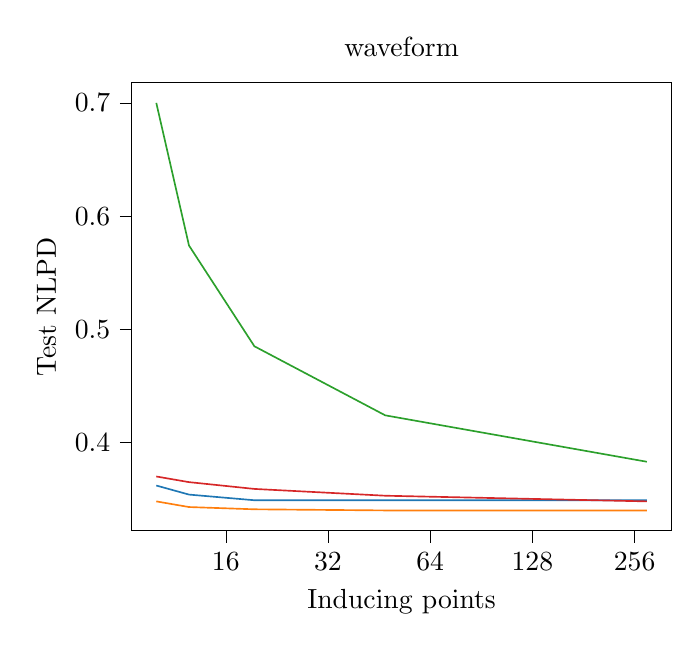
\begin{tikzpicture}

\definecolor{crimson2143940}{RGB}{214,39,40}
\definecolor{darkgray176}{RGB}{176,176,176}
\definecolor{darkorange25512714}{RGB}{255,127,14}
\definecolor{forestgreen4416044}{RGB}{44,160,44}
\definecolor{steelblue31119180}{RGB}{31,119,180}

\begin{axis}[
tick align=outside,
tick pos=left,
title={waveform},
x grid style={darkgray176},
xlabel={Inducing points},
xmin=4, xmax=268,
xtick style={color=black},
xtick={0,50,100,150,200,250,300},
xticklabels={0,16,32,64,128,256,},
y grid style={darkgray176},
ylabel={Test NLPD},
ymin=0.322, ymax=0.718,
ytick style={color=black}
]
\addplot [semithick, steelblue31119180]
table {%
16 0.362
32 0.354
64 0.349
128 0.349
256 0.349
};
\addplot [semithick, darkorange25512714]
table {%
16 0.348
32 0.343
64 0.341
128 0.34
256 0.34
};
\addplot [semithick, forestgreen4416044]
table {%
16 0.7
32 0.574
64 0.485
128 0.424
256 0.383
};
\addplot [semithick, crimson2143940]
table {%
16 0.37
32 0.365
64 0.359
128 0.353
256 0.348
};
\end{axis}

\end{tikzpicture}

  \end{minipage}
  \hfill
  \begin{minipage}[t]{.16\textwidth}
    \raggedleft
    % This file was created with tikzplotlib v0.10.1.
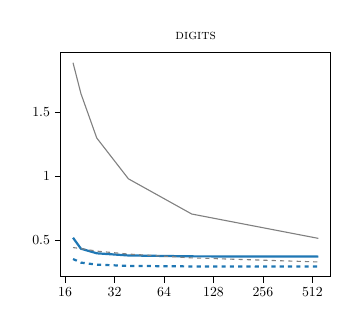
\begin{tikzpicture}[
scale=0.5
]

\definecolor{darkgray176}{RGB}{176,176,176}
\definecolor{gray}{RGB}{128,128,128}
\definecolor{steelblue31119180}{RGB}{31,119,180}

\begin{axis}[
tick align=outside,
tick pos=left,
title={\sc digits},
x grid style={darkgray176},
xmin=-8.8, xmax=536.8,
xtick style={color=black},
xtick={-100,0,100,200,300,400,500,600},
xticklabels={0,16,32,64,128,256,512,},
y grid style={darkgray176},
ymin=0.2101, ymax=1.9679,
ytick style={color=black}
]
\addplot [ultra thick, steelblue31119180]
table {%
16 0.516
32 0.43
64 0.394
128 0.377
256 0.37
512 0.368
};
\addplot [ultra thick, steelblue31119180, dashed]
table {%
16 0.349
32 0.321
64 0.305
128 0.295
256 0.291
512 0.29
};
\addplot [thick, gray]
table {%
16 1.888
32 1.646
64 1.298
128 0.978
256 0.702
512 0.511
};
\addplot [thick, gray, dashed]
table {%
16 0.439
32 0.431
64 0.411
128 0.388
256 0.358
512 0.326
};
\end{axis}

\end{tikzpicture}

  \end{minipage}
  \hfill
  \begin{minipage}[t]{.16\textwidth}
    \raggedleft
    % This file was created by tikzplotlib v0.9.8.
\begin{tikzpicture}

\definecolor{color0}{rgb}{0.274509803921569,0.509803921568627,0.705882352941177}
\definecolor{color1}{rgb}{1,0.549019607843137,0}

\begin{axis}[
height=\figureheight,
tick align=outside,
tick pos=left,
width=\figurewidth,
x grid style={white!69.0196078431373!black},
xlabel={\(\displaystyle M\) as \% of N},
xmin=-5, xmax=105,
xtick style={color=black},
xtick={-20,0,20,40,60,80,100,120},
xticklabels={\ensuremath{-}20,0,20,40,60,80,100,120},
y grid style={white!69.0196078431373!black},
ylabel={NLPD},
ymin=0.232868945885827, ymax=0.952205739288815,
ytick style={color=black},
ytick={0.2,0.4,0.6,0.8,1},
yticklabels={0.2,0.4,0.6,0.8,1.0}
]
\path [draw=color0, fill=color0, opacity=0.1]
(axis cs:1,0.391152761417344)
--(axis cs:1,0.321521954149105)
--(axis cs:2,0.282454703370333)
--(axis cs:5,0.294202713923217)
--(axis cs:10,0.26556607285869)
--(axis cs:15,0.2714883934195)
--(axis cs:20,0.267172403120068)
--(axis cs:40,0.2680998965525)
--(axis cs:60,0.268580750911881)
--(axis cs:60,0.31129434947327)
--(axis cs:60,0.31129434947327)
--(axis cs:40,0.337115320962889)
--(axis cs:20,0.345848237713317)
--(axis cs:15,0.326824039373233)
--(axis cs:10,0.331755020348582)
--(axis cs:5,0.342226542750507)
--(axis cs:2,0.346915562303046)
--(axis cs:1,0.391152761417344)
--cycle;

\path [draw=color1, fill=color1, opacity=0.1]
(axis cs:1,0.919508612315951)
--(axis cs:1,0.821918984692462)
--(axis cs:2,0.677101151550207)
--(axis cs:5,0.524269764776493)
--(axis cs:10,0.418282523447695)
--(axis cs:15,0.383338814008808)
--(axis cs:20,0.375641757595403)
--(axis cs:40,0.315946155255256)
--(axis cs:40,0.370004004383582)
--(axis cs:40,0.370004004383582)
--(axis cs:20,0.427686550442204)
--(axis cs:15,0.431995243421999)
--(axis cs:10,0.507855760482352)
--(axis cs:5,0.670933925464013)
--(axis cs:2,0.765602703537218)
--(axis cs:1,0.919508612315951)
--cycle;

\addplot [semithick, color0]
table {%
1 0.356337357783224
2 0.31468513283669
5 0.318214628336862
10 0.298660546603636
15 0.299156216396366
20 0.306510320416692
40 0.302607608757695
60 0.289937550192575
};
\addplot [semithick, color1]
table {%
1 0.870713798504207
2 0.721351927543713
5 0.597601845120253
10 0.463069141965024
15 0.407667028715403
20 0.401664154018804
40 0.342975079819419
};
\end{axis}

\end{tikzpicture}

  \end{minipage}\\[-1em]
  %
  % Legend  
  \definecolor{steelblue31119180}{RGB}{31,119,180}
  \definecolor{darkorange25512714}{RGB}{255,127,14}  
  \newcommand{\myline}[1]{\protect\tikz[baseline=-.5ex,line width=1.6pt]\protect\draw[draw=#1](0,0)--(1.2em,0);}
  \caption{Comparison of convergence in terms of number of inducing points $M$ in NLPD (mean over 10 seeds) on UCI classification tasks: \our (thick) vs.\ subsets (\cite{immer2021improving}, thin). Orange lines (\myline{darkorange25512714}) use the GP mean, whereas blue lines (\myline{steelblue31119180}) the NN MAP estimate as mean. Our \our converges fast for all cases.\looseness-1}
  \label{fig:uci}
  %\vspace*{-6pt}
\end{figure}



\subsection{Capturing uncertainty in UCI tasks under supervised learning}
\label{sec:uci}
%
We first evaluate \our on eight UCI benchmarks~\cite{UCI}, a variety of binary and multi-class classification tasks with different data set sizes.
We train a two-layer MLP for each of the classification tasks and follow the experiment set up in \cite{immer2021improving}.
%by using the same hyperparameters, performing a hyperparameter search over the prior precision $\delta$,
% We follow \cite{immer2021improving} by using the same hyperparameters, performing a hyperparameter search over the prior precision $\delta$,
% and run the experiment over $10$ random splits.
% That is, after training we construct the \our dual and use the resulting model for uncertainty quantification.
% for the neural network training as in the UCI experiments of
\cref{tbl:uci} (left) shows that \our with $M=256$ either matches or outperforms the predictive performance of the NN MAP, mean-field VI, Bayesian NN, and GLM
predictions %in terms of negative log-predictive density (NLPD).
(baselines from \cite{immer2021improving}).
That is, we match predictive performance despite being sparse.
%
In \cref{tbl:uci} (right) we compare to the subset GP method from \cite{immer2021improving} whilst using only $M=32$ inducing points.
It shows that \our is able to summarize the full data set more effectively than the GP subset method as it maintains predictive performance
whilst using fewer inducing points.
\cref{fig:uci} further shows that as the number of inducing points is lowered $M=512,\ldots, 16$, \our is able to maintain a much better NLPD than the GP subset.
These results demonstrate \our's sparse representation captures information from the entire data set and as a result provides good uncertainty estimates.
We provide further details of our experiments in \cref{app:uci}.
% as well as further results with varying number of inducing poitns ,64,128,256$
% We provide full details of our experiments as well as further experiments with varying number of inducing poitns and further results using $M=16,32,64,128,256$ in \cref{app:uci}.
% benefits of \our in summarizing the full data distribution onto a small set of inducing
% points over just picking a random subset.



% We match the predictive performance despite being sparse (here, $M=256$).


% This is
% However, our method used

% despite being sparse (here, $M=256$).

% (left), we compare our model to the NN MAP estimate, mean-field VI, a Bayesian NN, and a GLM model (see \cite{immer2021improving} for the baselines) in negative log-predictive density (NLPD).
% In \cref{tbl:uci} (left), we compare our model to the NN MAP estimate, mean-field VI, a Bayesian NN, and a GLM model (see \cite{immer2021improving} for the baselines) in negative log-predictive density (NLPD).
% We match the predictive performance despite being sparse (here, $M=256$).
% Results for $M=16,32,64,128,256$ are included in \cref{app:uci} with full experiment details.

% \cref{tbl:uci} (right) shows that \our is able to summarize the information of the full data set more efficiently than the sparse GP subset method.
% As a result, it maintains predictive performance whilst using fewer inducing points.
% This is even more apparent from \cref{fig:uci} which shows the benefits of \our in summarizing the full data distribution onto a small set of inducing points over just picking a random subset.

% In \cref{tbl:uci} (right), we also include an ablation and comparison study (to \cite{immer2021improving}) with a fixed low number of inducing points ($M=32$).
% The comparison shows that our sparse method is able to summarize the information of the full data set more efficiently than sparse subset methods, and can match the performance of the full GP even with a low number of inducing points. This is even more apparent from \cref{fig:uci} which shows the benefits of \our in summarizing the full data distribution onto a small set of inducing points over just picking a random subset.



% see \cref{tbl:uci} for a list of the datasets. The neural network training was done using MAP, with a prior $\mathcal{N}(0,\delta^{-1} \MI)$ with prior precision $\delta$. After training, we constructed the SVGP dual and used the resulting SVGP model for uncertainty quantification. Depending on task dimension and complexity, our model can match the NN MAP in NLPD performance even with a low number of inducing points, see \cref{tbl:uci}. We performed hyperparameter search over the prior precision, and ran the experiment over $10$ seeds. During the initial NN training, we used a learning rate of $1e-3$.

%\begin{figure}
%  \raggedleft\scriptsize
%  \setlength{\figurewidth}{\textwidth}
%  \setlength{\figureheight}{.55\figurewidth}
%  %\pgfplotsset{axis on top,ymajorgrids,axis line style={draw=none},legend style={at={(-.1,-.1)},anchor=north east}}
%  %\pgfplotsset{grid style={line width=.1pt, draw=gray!10,dashed}}
%  %\def\our{{\sc sfr} (ours)}
%  % This file was created with tikzplotlib v0.10.1.
\begin{tikzpicture}

\definecolor{crimson2143940}{RGB}{214,39,40}
\definecolor{darkgray176}{RGB}{176,176,176}
\definecolor{darkorange25512714}{RGB}{255,127,14}
\definecolor{darkturquoise23190207}{RGB}{23,190,207}
\definecolor{forestgreen4416044}{RGB}{44,160,44}
\definecolor{goldenrod18818934}{RGB}{188,189,34}
\definecolor{gray127}{RGB}{127,127,127}
\definecolor{lightgray204}{RGB}{204,204,204}
\definecolor{mediumpurple148103189}{RGB}{148,103,189}
\definecolor{orchid227119194}{RGB}{227,119,194}
\definecolor{sienna1408675}{RGB}{140,86,75}
\definecolor{steelblue31119180}{RGB}{31,119,180}

\begin{axis}[
height=\figureheight,
legend cell align={left},
legend style={fill opacity=0.8, draw opacity=1, text opacity=1, draw=lightgray204},
tick align=outside,
tick pos=left,
width=\figurewidth,
x grid style={darkgray176},
xmin=-0.2, xmax=4.2,
xtick style={color=black},
xtick={0,1,2,3,4},
xtick={0,1,2,3,4},
xtick={0,1,2,3,4},
xtick={0,1,2,3,4},
xtick={0,1,2,3,4},
xtick={0,1,2,3,4},
xtick={0,1,2,3,4},
xtick={0,1,2,3,4},
xtick={0,1,2,3,4},
xtick={0,1,2,3,4},
xtick={0,1,2,3,4},
xtick={0,1,2,3,4},
xtick={0,1,2,3,4},
xtick={0,1,2,3,4},
xtick={0,1,2,3,4},
xticklabels={256,512,1024,2048,3200},
xticklabels={256,512,1024,2048,3200},
xticklabels={256,512,1024,2048,3200},
xticklabels={256,512,1024,2048,3200},
xticklabels={256,512,1024,2048,3200},
xticklabels={256,512,1024,2048,3200},
xticklabels={256,512,1024,2048,3200},
xticklabels={256,512,1024,2048,3200},
xticklabels={256,512,1024,2048,3200},
xticklabels={256,512,1024,2048,3200},
xticklabels={256,512,1024,2048,3200},
xticklabels={256,512,1024,2048,3200},
xticklabels={256,512,1024,2048,3200},
xticklabels={256,512,1024,2048,3200},
xticklabels={256,512,1024,2048,3200},
y grid style={darkgray176},
ymin=-0.567324956290268, ymax=13.0270240820956,
ytick style={color=black}
]
\addplot [semithick, steelblue31119180]
table {%
0 2.450651686371
1 2.33688367659858
2 0.758006683252107
3 0.418063571567222
4 0.293906180967752
};
\addlegendentry{\sc GP subset}
\addplot [semithick, darkorange25512714]
table {%
0 1.12153317466841
1 0.85325292908048
2 12.4090991258054
3 0.0672844892936739
4 0.0627872786062761
};
\addlegendentry{\sc \our}
\addplot [semithick, forestgreen4416044]
table {%
0 1.30682946689449
1 1.27447684300892
2 0.0822643172822197
3 0.0732855173563596
4 0.0692346420741961
};
\addlegendentry{\sc GP subset (NN)}
\addplot [semithick, crimson2143940]
table {%
0 0.732772882751394
1 0.638123397907866
2 12.3951401856728
3 0.0738436001185355
4 0.0710273410515106
};
\addlegendentry{\sc \our (NN)}
\addplot [semithick, mediumpurple148103189, dashed]
table {%
0 1.6746972458165
1 1.6746972458165
2 1.6746972458165
3 1.6746972458165
4 1.6746972458165
};
\addlegendentry{\sc bnn}
\addplot [semithick, sienna1408675, dashed]
table {%
0 0.921512236735063
1 0.921512236735063
2 0.921512236735063
3 0.921512236735063
4 0.921512236735063
};
\addlegendentry{\sc glm}
\addplot [semithick, orchid227119194, dashed]
table {%
0 0.0677361758804467
1 0.0677361758804467
2 0.0677361758804467
3 0.0677361758804467
4 0.0677361758804467
};
\addlegendentry{\sc map}
\addplot [semithick, gray127]
table {%
0 0.0982
1 0.1364
2 0.7276
3 0.8718
4 0.9124
};
\addlegendentry{\sc GP subset}
\addplot [semithick, goldenrod18818934]
table {%
0 0.921
1 0.9598
2 0.0532
3 0.981
4 0.98
};
\addlegendentry{\sc \our}
\addplot [semithick, darkturquoise23190207]
table {%
0 0.9012
1 0.9088
2 0.9764
3 0.9764
4 0.9786
};
\addlegendentry{\sc GP subset (NN)}
\addplot [semithick, steelblue31119180]
table {%
0 0.971
1 0.97
2 0.0506
3 0.9778
4 0.9774
};
\addlegendentry{\sc \our (NN)}
\addplot [semithick, darkorange25512714, dashed]
table {%
0 0.7622
1 0.7622
2 0.7622
3 0.7622
4 0.7622
};
\addlegendentry{\sc bnn}
\addplot [semithick, forestgreen4416044, dashed]
table {%
0 0.9254
1 0.9254
2 0.9254
3 0.9254
4 0.9254
};
\addlegendentry{\sc glm}
\addplot [semithick, crimson2143940, dashed]
table {%
0 0.9788
1 0.9788
2 0.9788
3 0.9788
4 0.9788
};
\addlegendentry{\sc map}
\end{axis}

\end{tikzpicture}

%  \caption{Foo}
%  \label{fig:mnist}
%\end{figure}
%





\subsection{Supervised learning on image data sets}
\label{sec:image}
Similarly to the UCI experiments, we seek to demonstrate \our on image data that features more complicated data manifolds and model structures.
We consider the MNIST and Fashion-MNIST (FMNIST) classification tasks, and use an MLP and a CNN architecture respectively (matching the setup in \cite{immer2021improving}).
After training, we computed the duals for \our and use the model for prediction (full experiment details in \cref{app:image}).
In \cref{tbl:imagesuper}, we compare to baselines also used in \cite{immer2021improving}.
We report accuracy (ACC), NLPD, and expected calibration error (ECE).
For \our and the GP predictive subset method by \cite{immer2021improving}, we provide results when predicting with GP mean and when using the neural network (NN) and
fix the number of inducing points $M=1024$.
For completeness, we also include the GP predictive result from \cite{immer2021improving} which used more inducing points $M=3200$.
The results in \cref{tbl:imagesuper} agree with the conclusions drawn from the UCI experiments showing that \our is able to more efficiently capture the posterior using a sparse set of points.
They further demonstrate that \our's predictive mean (GP) significantly outperforms the GP predictive subset.
This is an interesting result as we cannot rely on the NN's prediction if we wish to condition on new data, using the dual conditioning from \label{sec:sequential}.
In this setting, we must rely on our GP's predictive mean.
% Other approaches, \cite{immer2021improving} never inten
% The resutls demonstrate that \our's predictive GP mean significantly outperforms the
These results on image data sets motivate experiments beyond the supervised learning setting, which we now detail.

% For \our and the GP predictive subset method by \cite{immer2021improving} we fix the number of points $M=1024$.



%We performed hyperparameter optimization over the prior precision, and found the optimal value to be [insert]. We ran the experiment over $5$ seeds. During the NN training, we used a batch size of $512$ and an Adam optimizer with learning rate $1e-3$.

%In addition to uncertainty estimates, our method can update the posterior when given new data. We gave the SVGP model 10 \% of the test dataset used for evaluation, and compare the performance of the SVGP model and the retrained NN in [INSERT TABLE]. 


\begin{table}[t!]
  \centering\scriptsize
  \caption{Metrics for supervised learning on image data with a CNN. We report accuracy, NLPD, and expected calibration error (mean$\pm$std) over 5 seeds. Our \our method is able to match the full methods using only a sparse set. For the GP predictive sparse subset method and \our we report results both using the NN MAP as mean (NN) and using the GP mean.}
	\label{tbl:imagesuper}
	% Control table spacing
	\renewcommand{\arraystretch}{1.}
	\setlength{\tabcolsep}{6pt}
	\setlength{\tblw}{0.095\textwidth}

	% Custom error formatting
	\newcommand{\val}[2]{%
		$#1$\textcolor{gray}{\tiny ${\pm}#2$}
	}

    % THE TABLE CAN BE FORMATTED MORE LIKE THIS
    % \begin{tabular}{l l C{\tblw} C{\tblw} C{\tblw} C{\tblw}}
    % \toprule
    % & Method & ACC~$\uparrow$ & NLPD~$\downarrow$ & ECE~$\downarrow$ & OOD-AUC~$\uparrow$  \\
    % \midrule
    % \multirow{2}{*}{FMNIST}
    % & MAP & \val{0.000}{0.000} & \val{0.000}{0.000} & \val{0.000}{0.000} & \val{0.000}{0.000} \\
    % & BNN predictive & \val{0.000}{0.000} & \val{0.000}{0.000} & \val{0.000}{0.000} & \val{0.000}{0.000} \\
    % & BNN predictive \cite{todo} & \val{0.000}{0.000} & \val{0.000}{0.000} & \val{0.000}{0.000} & \val{0.000}{0.000} \\
    % & GLM predictive & \val{0.000}{0.000} & \val{0.000}{0.000} & \val{0.000}{0.000} & \val{0.000}{0.000} \\
    % & GP predictive & \val{0.000}{0.000} & \val{0.000}{0.000} & \val{0.000}{0.000} & \val{0.000}{0.000} \\
    % & \our (NN) & \val{0.000}{0.000} & \val{0.000}{0.000} & \val{0.000}{0.000} & \val{0.000}{0.000} \\
    % & \our & \val{0.000}{0.000} & \val{0.000}{0.000} & \val{0.000}{0.000} & \val{0.000}{0.000} \\
    % \midrule
    % \multirow{2}{*}{CIFAR-10}
    % & MAP & \val{0.000}{0.000} & \val{0.000}{0.000} & \val{0.000}{0.000} & \val{0.000}{0.000} \\
    % & BNN predictive & \val{0.000}{0.000} & \val{0.000}{0.000} & \val{0.000}{0.000} & \val{0.000}{0.000} \\
    % & BNN predictive \cite{todo} & \val{0.000}{0.000} & \val{0.000}{0.000} & \val{0.000}{0.000} & \val{0.000}{0.000} \\
    % & GLM predictive & \val{0.000}{0.000} & \val{0.000}{0.000} & \val{0.000}{0.000} & \val{0.000}{0.000} \\
    % & GP predictive & \val{0.000}{0.000} & \val{0.000}{0.000} & \val{0.000}{0.000} & \val{0.000}{0.000} \\
    % & \our (NN) & \val{0.000}{0.000} & \val{0.000}{0.000} & \val{0.000}{0.000} & \val{0.000}{0.000} \\
    % & \our & \val{0.000}{0.000} & \val{0.000}{0.000} & \val{0.000}{0.000} & \val{0.000}{0.000} \\
    % \bottomrule
    % \end{tabular}
  \newcommand{\myline}{\protect\tikz[baseline=-.5ex,line width=.7pt]\protect\draw[draw=gray](0,0)--(7em,0);}
  \begin{tabular}{l c C{\tblw} C{\tblw} C{\tblw} C{\tblw} C{\tblw} C{\tblw}}
    \toprule
            &     &  \multicolumn{3}{c}{\myline~MNIST~\myline} & \multicolumn{3}{c}{\myline~FMNIST~\myline} \\
     Method & $M$ & ACC~$\uparrow$ & NLPD~$\downarrow$ & ECE~$\downarrow$ & ACC~$\uparrow$ & NLPD~$\downarrow$ & ECE~$\downarrow$ \\
    \midrule
    %\multirow{2}{*}{MNIST}
    MAP & -- & \val{98.22}{0.13} & \val{0.061}{0.004} & \val{0.006}{0.001}
          & \val{91.39}{0.11} & \val{0.258}{0.004} & \val{0.017}{0.001} \\
    BNN predictive \cite{immer2021improving} & -- & \val{93.14}{0.05} & \val{0.304}{0.002} & \val{0.111}{0.003}
                                               & \val{84.42}{0.12} & \val{0.942}{0.016} & \val{0.411}{0.008} \\
    BNN predictive \cite{ritter2018kfac} & -- & \val{93.03}{0.13} & \val{0.369}{0.003} & \val{0.168}{0.001}
                                           & \val{91.20}{0.07} & \val{0.265}{0.004} & \val{0.024}{0.002} \\
    GLM predictive \cite{immer2021improving} & -- & \val{98.40}{0.05} & \val{0.054}{0.002} & \val{0.007}{0.001}
                                               & \val{92.25}{0.10} & \val{0.244}{0.003} & \val{0.012}{0.003} \\\arrayrulecolor{black!10}\midrule
    GP predictive \cite{immer2021improving} & $3200$ & \val{\textbf{98.22}}{0.13} & \val{\textbf{0.058}}{0.001} & \val{\textbf{0.003}}{0.000}
                                                     & \val{91.36}{0.11} & \val{\textbf{0.25}}{0.004} & \val{\textbf{0.007}}{0.001} \\

    GP predictive (NN) & $1024$ & \val{97.70}{0.07} & \val{0.080}{0.002} & \val{0.011}{0.001}
                              & \val{\textbf{91.47}}{0.41} & \val{0.289}{0.009} & \val{0.033}{0.003} \\

    GP predictive & $1024$  & \val{76.28}{1.85} & \val{0.702}{0.029} & \val{0.070}{0.022}
                            & \val{83.98}{0.35} & \val{0.503}{0.012} & \val{0.052}{0.006} \\
    \our (NN) & $1024$ &  \val{98.02}{0.12} & \val{0.066}{0.003} & \val{0.007}{0.001}
                     & \val{\textbf{91.93}}{0.45} & \val{0.267}{0.011} & \val{0.028}{0.003} \\
    \our & $1024$ & \val{\textbf{98.07}}{0.06} & \val{0.063}{0.003} & \val{0.005}{0.001}
                  & \val{\textbf{91.56}}{0.35} & \val{\textbf{0.253}}{0.006} & \val{0.012}{0.001} \\
%    \multirow{2}{*}{FMNIST}
%    & MAP & \val{91.39}{0.11} & \val{0.258}{0.004} & \val{0.017}{0.001} \\
    %& BNN predictive \cite{immer2021improving} & \val{84.42}{0.12} & \val{0.942}{0.016} & \val{0.411}{0.008} \\
    % & BNN predictive \cite{ritter2018kfac} & \val{91.20}{0.07} & \val{0.265}{0.004} & \val{0.024}{0.002} \\
    % & GLM predictive \cite{immer2021improving} & \val{92.25}{0.10} & \val{0.244}{0.003} & \val{0.012}{0.003} \\
    %& GP predictive \cite{immer2021improving} $m=3200$ & \val{91.36}{0.11} & \val{0.25}{0.004} & \val{0.007}{0.001} \\
    % & GP predictive NN $m=1024$ &  \val{0}{0.07} & \val{0}{0.002} & \val{0}{0.001} \\
    % & GP predictive $m=1024$  &  \val{0}{1.85} & \val{0}{0.029} & \val{0}{0.022} \\
    % & \our NN $m=1024$ &  \val{0}{0.0} & \val{0}{0.003} & \val{0}{0.001} \\
    % & \our $m=1024$ &  \val{0}{0.06} & \val{0}{0.003} & \val{0}{0.001} \\
    \arrayrulecolor{black}
    \bottomrule
  \end{tabular}

% & \sc \sc gp predictive  &  \val{76.28333}{1.849} & \val{0.70168}{0.02883} & \val{0.07049}{0.02154} \\
% & \sc \sc gp predictive NN \cite{immer2021improving} &  \val{97.70333}{0.074} & \val{0.08027}{0.00248} & \val{0.01052}{0.00097} \\
% & \sc \our &  \val{98.06667}{0.060} & \val{0.06312}{0.00284} & \val{0.00493}{0.00086} \\
% & \sc \our NN &  \val{98.02000}{0.122} & \val{0.06583}{0.00294} & \val{0.00714}{0.00096} \\
% M=512
% & \sc \our &  \val{96.05}{0.00} & \val{0.85}{0.01} & \val{0.50}{0.00} \\
% & \sc \sc gp predictive  &  \val{14.79}{0.01} & \val{2.30}{0.02} & \val{0.02}{0.01} \\
% & \sc \sc gp predictive NN \cite{immer2021improving} &  \val{91.49}{0.01} & \val{1.25}{0.01} & \val{0.61}{0.00} \\
% & \sc \our NN &  \val{96.96}{0.00} & \val{0.63}{0.00} & \val{0.40}{0.00} \\

% M=1024

    % THE TABLE NUMBER ARE GENERATED BY A SCRIPT
	%\begin{tabular}{l C{0.6\tblw} C{0.6\tblw} C{0.6\tblw} C{0.6\tblw} C{0.6\tblw}  C{0.6\tblw}}
\toprule
& acc & nll & ece & ood-auc  \\
\midrule
\sc FMNIST and MAP & \val{91.39}{0.11} & \val{0.258}{0.004} & \val{0.017}{0.001} & \val{0.864}{0.014} \\
\sc FMNIST and BNN predictive & \val{84.42}{0.12} & \val{0.942}{0.016} & \val{0.411}{0.008} & \val{0.945}{0.002} \\
\sc FMNIST and BNN predictive (Ritter et al.) & \val{91.2}{0.07} & \val{0.265}{0.004} & \val{0.024}{0.002} & \val{0.947}{0.006} \\
\sc FMNIST and GLM predictive & \val{92.25}{0.1} & \val{0.244}{0.003} & \val{0.012}{0.003} & \val{0.955}{0.006} \\
\sc FMNIST and GP predictive & \val{91.36}{0.11} & \val{0.25}{0.004} & \val{0.007}{0.001} & \val{0.918}{0.01} \\
\sc FMNIST and SVGP (500) & \val{90.224}{0.656} & \val{0.292}{0.01} & \val{0.048}{0.002} & \val{0.0}{0.0} \\
\bottomrule
\end{tabular}

\end{table}


\subsection{Updating the network representation in continual learning}
\label{sec:cl-exp}
%
%%% Very rough draft
%This experiment's section is meant to demonstrate the quality of our sparse representation to retain previous knowledge in the Continual learning setting. Unfortunately the CL literature is based on methods that require very diverse set of hyperparameters 
%% Idea: it is very difficult to have everything under control, because model changes, settings change, optimizer change, and so on. Then what we did was trying to replicate as close as possible the results for the competing methods by using their codebases where available and choosing the hyperpameters accordingly to their choices.
%
%% Why SH?
%% TODO: there are at least two papers that clearly say MH is unrealistic and too simple as a consequence is not a good way to assess the quality of the method
%
%% Architectures
%We conduct the experiments on a set of three CL benchmarks Sequential-MNIST (S-MNIST), Sequential-FashionMNIST (S-FMNIST), and Permuted-MNIST (P-MNIST).  Following \cite{rudner2022continual, pan2020continual}, we used a two-layer MLP with 256 hidden units with ReLU activation for S-MNIST and S-FMNIST, and a two-layer with 100 hidden units for P-MNIST. 
%
%% Methods
%We compared our method to 1) weight-regularization based methods EWC, SI and VCL (which also has the addition of coresets); 2) function-based regularization based methods DER, FROMP, S-FSVI, SFR; 3) an ablation for which we replace $\bar{\MB}^{-1}$ with an identity matrix $\MI_m$, \ie which is equivalent to assuming a GP with iid realization \todo{Not sure this is 100$\%$ correct}.
%% Inducing points
%Following \citep{rudner2022continual}, we use 200 inducing points per tasks % this one can be difficult to justify since S-FSVI samples 200 context points and then iteratively samples 40 coresets points (or at least that's what I got)
%on all the inducing points, and a lower number of inducing point for S-MNIST, to investigate if our method was still capable of capture more information due to its sparse formulation, as explained in \cref{todo}.
%
%%% Questions: Should we also mention the Identity outside when not trained on those classes or just leave that for the appendix?



\setlength{\columnsep}{8pt}
\setlength{\intextsep}{0pt}
\begin{wraptable}{R}{.65\textwidth}
  \centering\scriptsize
  \caption{Continual learning experiments. We report accuracy${\pm}$std and bold based on a $t$-test. $^*$Methods rely on weight regularization.}
  %\textcolor{blue}{Results from \cite{rudner2022continual}
  %\color{red}{Preliminary results need more runs or hyperparam tuning}
	\label{tbl:cl_table_1}
	
	% Control table spacing
	\renewcommand{\arraystretch}{1.}
	\setlength{\tabcolsep}{1pt}
	\setlength{\tblw}{0.14\textwidth}  
	
	% Custom error formatting
	\newcommand{\val}[2]{%
		$#1$\textcolor{gray}{\tiny ${\pm}#2$}
	} 
	
	\vspace*{-4pt}
	
	% Import table content
	\begin{tabular}{@{}lcccc@{}}
\toprule
 Method           & 
\begin{tabular}[c]{c}S-MNIST (SH) \\ 40 points\end{tabular} & 
\begin{tabular}[c]{c}S-MNIST (SH) \\ 200 points\end{tabular} & 
\begin{tabular}[c]{c}S-FMNIST (SH)\\ 200 points\end{tabular} & 
\begin{tabular}[c]{c}P-MNIST (SH) \\ 200\end{tabular} \\ \midrule
%% Weight Regularization Methods
{\sc Online-EWC}~\cite{schwarz2018progress}$^*$ & \val{19.95}{0.28} & \val{19.95}{0.28} & \val{19.48}{0.01} & \val{74.87}{1.81}\\
{\sc SI}~\cite{zenke2017continual}$^*$ & \val{19.82}{0.09} & \val{19.82}{0.09} & \val{19.80}{0.21} & \val{88.39}{1.37}\\
{\sc VCL}~\cite{nguyen2018variational} & \val{}{} & \color{blue}{\val{32.11}{1.16}} & \val{48.35}{} &  \val{92.84}{0.34}\\
%{\sc VCL} (no coreset) & \val{}{} & \color{blue}{\val{17.74}{1.20}} & \val{}{} & \color{blue}{\val{87.50}{0.61}}\\
\midrule
%% Functional Regularization Methods
{\sc DER}~\cite{buzzega2020dark} & \val{85.26}{0.54} & \val{92.13}{0.45} & \val{82.03}{0.57} & \val{91.53}{0.26} \\
{\sc FROMP}~\cite{pan2020continual} & \val{75.21}{2.05} & \val{89.54}{0.72} & \val{78.83}{0.46} & \color{blue}{\val{94.90}{0.04}} \\
{\sc S-FSVI}~\cite{rudner2022continual} & \val{84.51}{1.30} & \color{blue}{\val{92.87}{0.14}} & \val{77.54}{0.40} & \color{blue}{\val{95.76}{0.02}} \\
{\sc SFR}~(Ours) & \val{88.73}{0.31} & \val{94.11}{0.15} & \val{81.71}{0.57} & \val{94.95}{0.14}\\
%{\sc L2} & \val{87.48}{0.81} & \val{93.98}{0.17} & \val{81.20}{0.30} & \val{93.89}{0.07}\\
{\sc -- L2} & \val{88.14}{0.86} & \val{93.90}{0.05} & \val{81.21}{0.36} & \val{94.54}{0.11}\\
\bottomrule
\end{tabular}

\end{wraptable}
%
% Overview
We show how the regularizer described in \cref{sec:sequential} can be used in continual learning to retain a compact representation of the neural network.
The experiments are run only in the single-head (SH) setting that is harder and more realistic than multi-head (MH) (see discussion in \citep{van2019three}).	
% Benchmarks/architectures
 Our regularizer is evaluated on three CL benchmarks, specifically Split-MNIST (S-MNIST), Split-FashionMNIST (S-FMNIST), and the 10-tasks Permuted-MNIST (P-MNIST). We adhere to the same setups outlined in \cite{rudner2022continual, pan2020continual}, which use a two-layer MLP with 256 hidden units and ReLU activation for S-MNIST and S-FMNIST and a two-layer MLP with 100 hidden units for P-MNIST, to ensure consistency (see \cref{app:cl-exp} for full details).

% Methods
We compare our method against two categories of methods: {\em (i)}~weight-regularization methods: EWC, SI, and VCL (with coresets), and {\em(ii)}~function-based regularization methods: DER, FROMP, and S-FSVI. We also introduce an ablation study where we replace our $\bar{\MB}_t^{-1}$ with an identity matrix $\MI_M$, equivalent to having an L2 regularization between current and old function outputs.
In \cref{tbl:cl_table_1}, we use 200 points for each task, and we further demonstrate our method's ability to compress the task data set information on a lower number of points for S-MNIST.

%% Comments on the results:
From \cref{tbl:cl_table_1}, it is clear that the weight-space regularization methods fail entirely compared to the function-space methods on S-MNIST and S-FMNIST but are still comparable on P-MNIST.
Considering only function-space methods, we can see that \our achieves the best results on most data sets and is particularly effective when using fewer points per task.
On S-FMNIST, our method obtains close results to DER, which regularizes the model by taking the mean squared error between current and old function outputs without accounting for the covariance structure of the loss similar to our L2 ablation. However, DER resorts to a reservoir sampling \citep{vitter1985random} that continuously update the set of points instead of selecting them at the task boundary.
The \our-based regularizer obtains comparable results to the best-performing method on P-MNIST, S-FSVI, which requires heavy computations compared to \our to perform variational inference. Finally, it is worth noticing as our ablation already provides a very solid baseline consistently over all data sets.





\subsection{Reinforcement learning under sparse rewards}
\label{sec:rl-exp}
% We now demonstrate the quaility of \our's uncertainty estimates by showing that it can improve sample efficiency in RL.
% Balancing the trade-off between exploration and exploitation is a key challenge in RL \cite{sutton2018reinforcement}.
% Should an agent select actions that it knows will lead to high reward (exploitation), or actions which it has not select before in the
% hope to discover new high reward actions (exploration)?

% when used in conjuction with an
% uncertainty-guided exploration strategy.


% In this section, we show that \our's uncertainty estimates can be used to balance this trade-off in a model-based RL algorithim,
% demonstrating the quality of our uncertainty estimates.

% A key challenge in RL is balancing the trade-off between exploration and exploitation.
% That is, should an agent select actions that it knows will lead to high reward (exploitation), or should it
% select new ones in hope to discover actions leading to higher reward (exploration).
% One promising direction is to model the uncertainty associated with a learned transition dynamics and use it to guide exploration.
% Prior work has learned dynamics models using GPs \cite{deisenrothPILCO2011,kamtheDataEfficient2018},
% ensembles of neural networks \cite{curiEfficient2020,chuaDeepReinforcementLearning2018}
% and variational inference \cite{galImproving2016,houthooftVIME2017}.
% There are then many ways to leverage uncertainty in model-based RL, for example,
% taking an expectation over epistemic uncertainty  \cite{deisenrothPILCO2011,kamtheDataEfficient2018,chuaDeepReinforcementLearning2018},
% sampling from the posterior, akin to Thompson sampling but referred to as posterior sampling RL
% \cite{osbandMoreEfficientReinforcement2013},
% and methods based on upper confidence bounds (UCB) \cite{curiEfficient2020}.

% Make custom TikZ command (argument: colour)
\newcommand{\lab}[1]{\protect\tikz[baseline=-.5ex]{\protect\node[minimum width=1.5em,minimum height=.8em,fill=#1,opacity=.1](a){};\protect\draw[#1,semithick](a.west)--(a.east);}}

% The methods
\definecolor{darkgray176}{RGB}{176,176,176} % darkgray176
\definecolor{color-our}{RGB}{0,191,191} %darkturquoise0191191
\definecolor{color-mlp}{RGB}{191,0,191} % darkviolet1910191
\definecolor{color-ddpg}{RGB}{191,191,0} % goldenrod1911910
\definecolor{color-ensemble}{RGB}{0,127,0} % green01270
\definecolor{lightgray204}{RGB}{204,204,204} % lightgray204



As a final experiment, we demonstrate the capability of \our to use its uncertainty estimates as guidance for exploration in model-based reinforcement learning (RL); this serves as a practical test to the quality of our uncertainty estimates. We use \our to help learn a dynamics model within a model-based RL strategy that employs posterior sampling to guide exploration \cite{osbandMoreEfficientReinforcement2013,osbandWhyPosteriorSampling2017}.
%
We use the cartpole swingup task in MuJoCo \cite{todorov2012mujoco}, a classic benchmark for nonlinear control (see \cref{fig:rl}).
The goal is to swing the pole up and balance it around the upward position.
We increase the difficulty of exploration by using a sparse reward function.
See \cref{app:rl} for an overview of the reinforcement learning problem, details of the algorithm, and the experiment setup.


%\cref{fig:rl} shows training curves using \our as the dynamic model (cyan) as well as a Laplace-GGN with GLM predictions (red), an ensemble of neuralnetworks (green) and a basic MLP wih no uncertainty (magenta). To ensure a fair comparison, we use the same MLP architecture/training scheme and use them in the same model-based RL algorithm, detailed in \cref{app:rl}. We also compare to deep deterministic policy gradient (DDPG) \cite{lillicrapContinuousControlDeep2016}, a model-free RL algorithim (yellow). The training curves show that \our's uncertainty estimates are useful for guiding exploration as it converges in fewer episodes, i.e. it is more sample efficient. As expected, the MLP strategy (without uncertainty) was not able to successfuly explore the environment.(), (\lab{color-mlp}),

\cref{fig:rl} shows training curves for using \our as the dynamic model (\lab{color-our}), along with a Laplace-GGN~\cite{immer2021scalable} with GLM predictions (\lab{red}), an ensemble of neural networks (\lab{color-ensemble}), and a basic MLP without uncertainty (\lab{color-mlp}). To ensure a fair comparison, we maintain the same MLP architecture/training scheme across all these methods and incorporate them into the same model-based RL algorithm (see \cref{app:rl}). We also compare our results with Deep Deterministic Policy Gradient (DDPG, \cite{lillicrapContinuousControlDeep2016}), a model-free RL algorithm (\lab{color-ddpg}).
The training curves show that \our's uncertainty estimates help exploration as it converges in fewer episodes, demonstrating higher sample efficiency.
As expected, the MLP strategy (without uncertainty) was not able to successfuly explore the environment.\looseness-2


% We compare \our (cyan) to a Laplace-GGN with GLM predictions (red), an ensemble of neural networks (green) and a basic MLP wih no uncertainty (magenta).
% To ensure a fair comparison, we use the same MLP architecture/training scheme and use them in the same model-based RL algorithm, detailed in \cref{app:rl}.
% See \cref{app:rl} for more details of our experiments.
% As expected DDPG is the least sample inefficient
% The training curves in \cref{fig:rl} show that \our's uncertainty estimates are useful for guiding exploration as it converges in fewer episodes.

% \cite{deisenrothPILCO2011},
% Posterior sampling


% based on

% Model-based RL algorithims are more sample efficient than their model-free counterparts as they learn a model of the transition dynamics and
% use it to augment the RL loop.


% Prior work has used show that modelling uncertainty in the transition dynamics can further improve exploration and thus sample efficiency.
% For example, with GPs \cite{deisenrothPILCO2011,kamtheDataEfficient2018},
% ensembles of neural networks \cite{curiEfficient2020,chuaDeepReinforcementLearning2018}
% and variational inference \cite{galImproving2016,houthooftVIME2017}

% We now demonstrate the quaility of \our's uncertainty estimates by showing that it can improve sample efficiency in RL.

% In this section, we show that \our's uncertainty estimates can be used to balance this trade-off in a model-based RL algorithim,
% demonstrating the quality of our uncertainty estimates.
% In this section, we demonstrate  that our method's principled uncertainty estimates can be used to balance this trade-off in a model-based RL algorithim.

% It is an inherently unstable and underactuated mechanical system.

% by using it to learn a dynamics model and
% evaluate the
% We test \our by using it to learn a dynamics model
% our method on the cart pole swing up task in MuJoCo \cite{todorov2012mujoco}, a classic benchmark for nonlinear control, see \cref{fig:rl}.
% The goal is to swing the pole up and balance it around the upward position.
% We increase the  difficulty of exploration in this environment by using a sparse reward function.


% We compare our method to a Laplace-GGN with GLM predictions (red), an ensemble of neural networks (green) and a basic MLP wih no uncertainty (magenta).
% To ensure a fair comparison, we use the same MLP architecture/training scheme and use them in the same model-based RL algorithm, detailed in \cref{app:rl}.
% % See \cref{app:rl} for more details of our experiments.
% We also compare to deep deterministic policy gradient (DDPG) \cite{lillicrapContinuousControlDeep2016}, a model-free RL algorithim (yellow).
% % As expected DDPG is the least sample inefficient
% The training curves in \cref{fig:rl} show that \our's uncertainty estimates are good for exploration as it converges in fewer episodes.

% We compare our method with deep deterministic policy gradient (DDPG) \cite{lillicrapContinuousControlDeep2016} -- a model-free RL baseline --
% which is sample inefficient.



\begin{figure}[!t]
 \centering\scriptsize
 \begin{subfigure}[c]{.24\textwidth}
 \centering
 \textbf{Cartpole swingup setup}\\[1em]
 \resizebox{\textwidth}{!}{%
 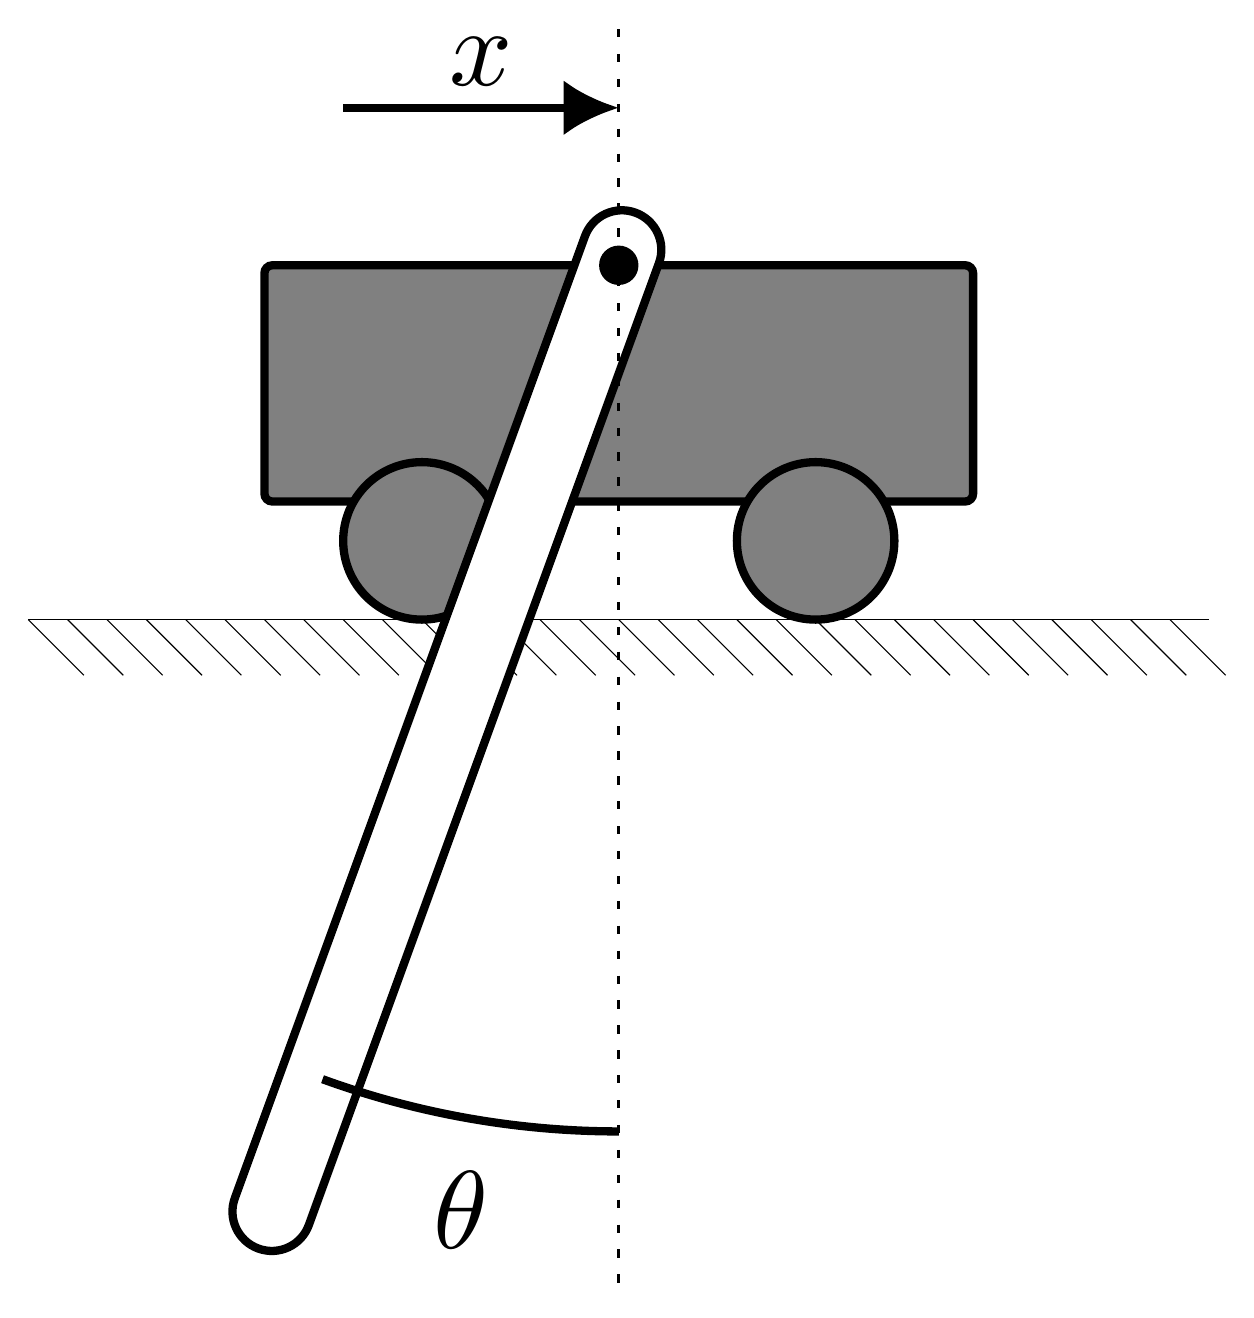
\begin{tikzpicture}[inner sep=0,outer sep=0]

   % Draw decorated 'ground'
   \draw[postaction={draw, decorate, decoration={border, angle=-45,
					amplitude=1cm, segment length=.5cm}}] (-3,-1.5) -- (12,-1.5);

   % The cart
   \draw[draw=black,fill=black!50,draw=black,line width=3pt,rounded corners=1mm] (0,0) rectangle (9cm,3cm);
   \node[fill=black,circle,minimum size=.5cm] (dot) at (4.5cm,3cm) {};

   % Wheels
   \node[fill=white,draw=black,line width=3pt,circle,minimum size=2cm,,fill=black!50] at (2cm,-.5cm) {};
   \node[fill=white,draw=black,line width=3pt,circle,minimum size=2cm,fill=black!50] at (7cm,-.5cm) {};

   % The arm
   \node[anchor=north,minimum width=1cm,minimum height=14cm,draw=black,rotate=-20,rounded corners=5mm,yshift=7mm,xshift=-.3mm,fill=white,draw=black,line width=3pt] at (dot) {};
   \node[fill=black,circle,minimum size=.5cm] at (dot) {};

   % Markings
   \draw[loosely dashed,line width=1pt] (4.5,6) -- (4.5,-10);

   % Arrow
   \draw[->,black,line width=3pt,-{Latex[length=7mm,width=7mm]}] (1,5) --node[above,outer sep=8pt]{\scalebox{4}{$x$}} (4.5,5);

   \def\centerarc[#1](#2)(#3:#4:#5)% Syntax: [draw options] (center) (initial angle:final angle:radius)
   { \draw[#1] ($(#2)+({#5*cos(#3)},{#5*sin(#3)})$) arc (#3:#4:#5); }

   % Draw arc
   \centerarc[black,line width=3pt](dot)(250:270:11)
   \node at (2.5,-9) {\scalebox{4}{$\theta$}};

   %\node[white,minimum size=1cm] at (4.5,-13) {};

 \end{tikzpicture}}\\[2em]~
 \end{subfigure}
 \hfill
 \begin{subfigure}[c]{.7\textwidth}
   \raggedleft\scriptsize
   \setlength{\figurewidth}{\textwidth}
   \setlength{\figureheight}{.55\figurewidth}
   \pgfplotsset{axis on top,ymajorgrids,axis line style={draw=none},legend style={at={(-.1,-.1)},anchor=south east}}
   \pgfplotsset{grid style={line width=.1pt, draw=gray!10,densely dotted}}
   \hspace*{-1.7cm}%
   \def\our{{\sc sfr} (ours)}
   % This file was created with tikzplotlib v0.10.1.
\begin{tikzpicture}

\definecolor{darkgray176}{RGB}{176,176,176}
\definecolor{darkturquoise0191191}{RGB}{0,191,191}
\definecolor{darkviolet1910191}{RGB}{191,0,191}
\definecolor{goldenrod1911910}{RGB}{191,191,0}

\begin{axis}[
height=\figureheight,
tick align=outside,
width=\figurewidth,
x grid style={darkgray176},
xlabel={Episode},
xmajorticks=false,
xmin=0, xmax=70,
xtick style={color=black},
y grid style={darkgray176},
ylabel={Return},
ymajorticks=false,
ymin=-20.4201265880636, ymax=428.822658349336,
ytick style={color=black}
]
\path [draw=darkturquoise0191191, fill=darkturquoise0191191, opacity=0.2]
(axis cs:0,0)
--(axis cs:0,0)
--(axis cs:1,8.88178419700125e-16)
--(axis cs:2,19.1973059533824)
--(axis cs:3,2.70921953514345)
--(axis cs:4,0)
--(axis cs:5,0.451092962245884)
--(axis cs:6,6.96399518367128)
--(axis cs:7,7.07526404924361)
--(axis cs:8,8.43594417646889)
--(axis cs:9,36.0887175252979)
--(axis cs:10,27.366456892827)
--(axis cs:11,26.3152073519428)
--(axis cs:12,40.8775744160779)
--(axis cs:13,47.2932308609594)
--(axis cs:14,68.7357615602261)
--(axis cs:15,74.4041517095617)
--(axis cs:16,86.0987773365824)
--(axis cs:17,137.775325010921)
--(axis cs:18,170.180368869445)
--(axis cs:19,246.562436247929)
--(axis cs:20,248.163506907404)
--(axis cs:21,269.646382052957)
--(axis cs:22,174.922627793507)
--(axis cs:23,236.699250575024)
--(axis cs:24,184.169901628923)
--(axis cs:25,260.517848576535)
--(axis cs:26,304.245690212262)
--(axis cs:27,238.520053707758)
--(axis cs:28,158.414590869285)
--(axis cs:29,272.611511061667)
--(axis cs:30,204.580740575742)
--(axis cs:31,314.521994629042)
--(axis cs:32,299.442239887491)
--(axis cs:33,275.115019539309)
--(axis cs:34,348.382066025368)
--(axis cs:35,363.274460850735)
--(axis cs:36,344.35941483396)
--(axis cs:37,364.403898001892)
--(axis cs:38,345.472645448431)
--(axis cs:39,359.173726715519)
--(axis cs:40,385.532686896454)
--(axis cs:41,336.973949643389)
--(axis cs:42,376.728630822865)
--(axis cs:43,268.808750288614)
--(axis cs:44,390.874191206634)
--(axis cs:45,384.494098723921)
--(axis cs:46,375.653225022356)
--(axis cs:47,341.958565967325)
--(axis cs:48,387.897118515591)
--(axis cs:49,377.871057436404)
--(axis cs:50,376.61337000803)
--(axis cs:51,376.104153883634)
--(axis cs:52,375.416150236303)
--(axis cs:53,364.550455035162)
--(axis cs:54,387.77933956538)
--(axis cs:55,386.573621424696)
--(axis cs:56,355.486468060268)
--(axis cs:57,372.077103651552)
--(axis cs:58,388.13826690375)
--(axis cs:59,363.883959642548)
--(axis cs:60,390.171932483887)
--(axis cs:61,387.576652101937)
--(axis cs:62,386.281827763581)
--(axis cs:63,379.85256860698)
--(axis cs:64,384.537570802637)
--(axis cs:65,379.635359061115)
--(axis cs:66,381.907054016017)
--(axis cs:67,375.071248940094)
--(axis cs:68,384.623693136768)
--(axis cs:68,400.614148660107)
--(axis cs:68,400.614148660107)
--(axis cs:67,392.0207798685)
--(axis cs:66,397.73206951914)
--(axis cs:65,393.73470929826)
--(axis cs:64,397.41932617002)
--(axis cs:63,393.616083736771)
--(axis cs:62,396.613130732513)
--(axis cs:61,397.163093991813)
--(axis cs:60,398.740897105956)
--(axis cs:59,387.553857740264)
--(axis cs:58,396.218422549375)
--(axis cs:57,392.989461289854)
--(axis cs:56,391.066058795201)
--(axis cs:55,396.904112950304)
--(axis cs:54,398.735723911182)
--(axis cs:53,396.810921917963)
--(axis cs:52,402.608825349635)
--(axis cs:51,399.317879807772)
--(axis cs:50,392.851522570095)
--(axis cs:49,396.473193051878)
--(axis cs:48,399.680383925815)
--(axis cs:47,400.070151073691)
--(axis cs:46,404.974118727644)
--(axis cs:45,406.842314850298)
--(axis cs:44,400.414358598053)
--(axis cs:43,392.814436967246)
--(axis cs:42,395.707367712291)
--(axis cs:41,395.927686098799)
--(axis cs:40,402.708914666046)
--(axis cs:39,402.82099984698)
--(axis cs:38,389.101219297663)
--(axis cs:37,403.923238228577)
--(axis cs:36,389.207626181665)
--(axis cs:35,400.147194422703)
--(axis cs:34,390.749110732444)
--(axis cs:33,374.53565184741)
--(axis cs:32,376.617495219931)
--(axis cs:31,385.416207275255)
--(axis cs:30,319.590276880313)
--(axis cs:29,336.59080827427)
--(axis cs:28,300.109415020608)
--(axis cs:27,353.355056155523)
--(axis cs:26,354.78533395766)
--(axis cs:25,365.052027522097)
--(axis cs:24,332.553889874984)
--(axis cs:23,317.861369542163)
--(axis cs:22,269.578251112743)
--(axis cs:21,351.910124294699)
--(axis cs:20,322.623285084784)
--(axis cs:19,332.05288357629)
--(axis cs:18,264.88169167743)
--(axis cs:17,268.359167481755)
--(axis cs:16,213.382967811123)
--(axis cs:15,160.966517846102)
--(axis cs:14,180.589569555497)
--(axis cs:13,87.3792743270289)
--(axis cs:12,92.8039540568225)
--(axis cs:11,107.459110580186)
--(axis cs:10,80.3550569507094)
--(axis cs:9,62.0083010026867)
--(axis cs:8,20.9274324409627)
--(axis cs:7,23.0396739237789)
--(axis cs:6,20.104176889693)
--(axis cs:5,24.7621135673714)
--(axis cs:4,0)
--(axis cs:3,12.2629842917608)
--(axis cs:2,39.4896126867543)
--(axis cs:1,9.8411262512207)
--(axis cs:0,0)
--cycle;

\path [draw=blue, fill=blue, opacity=0.2]
(axis cs:0,0)
--(axis cs:0,0)
--(axis cs:1,8.88178419700125e-16)
--(axis cs:2,3.78919723743713)
--(axis cs:3,4.60948931875786)
--(axis cs:4,8.88178419700125e-16)
--(axis cs:5,0.551723850423719)
--(axis cs:6,13.1887119818137)
--(axis cs:7,17.69092802924)
--(axis cs:8,12.4874299420715)
--(axis cs:9,2.11898013700558)
--(axis cs:10,1.67976053696799)
--(axis cs:11,13.7100193510876)
--(axis cs:12,19.3686063248268)
--(axis cs:13,23.8082359506491)
--(axis cs:14,28.7681558109863)
--(axis cs:15,28.463491440406)
--(axis cs:16,32.5464599886542)
--(axis cs:17,40.7538967430292)
--(axis cs:18,31.6785665236504)
--(axis cs:19,49.0896912424828)
--(axis cs:20,91.8498794830312)
--(axis cs:21,77.199697520426)
--(axis cs:22,98.2210797608253)
--(axis cs:23,140.366366754263)
--(axis cs:24,134.960998085603)
--(axis cs:25,121.940111638805)
--(axis cs:26,168.928892121208)
--(axis cs:27,199.702033216643)
--(axis cs:28,189.063034934935)
--(axis cs:29,271.372654810407)
--(axis cs:30,287.023800144222)
--(axis cs:31,327.420651938715)
--(axis cs:32,211.174386922893)
--(axis cs:33,204.498879716404)
--(axis cs:34,273.306470498059)
--(axis cs:35,253.9410204196)
--(axis cs:36,348.887512370934)
--(axis cs:37,373.113150532198)
--(axis cs:38,345.621671749785)
--(axis cs:39,384.091143446146)
--(axis cs:40,359.64684260537)
--(axis cs:41,375.017243629353)
--(axis cs:42,377.803229462724)
--(axis cs:43,357.462029012615)
--(axis cs:44,376.380044142874)
--(axis cs:45,373.314458237396)
--(axis cs:46,370.063881541742)
--(axis cs:47,370.030976971574)
--(axis cs:48,362.218684795274)
--(axis cs:49,369.265434097604)
--(axis cs:50,353.24032361145)
--(axis cs:51,375.663528830786)
--(axis cs:52,354.295555267299)
--(axis cs:53,381.39158199575)
--(axis cs:54,385.158706980437)
--(axis cs:55,386.67687265099)
--(axis cs:56,384.16319558511)
--(axis cs:57,386.51532083829)
--(axis cs:58,391.996122760009)
--(axis cs:59,391.72064053588)
--(axis cs:60,386.686547542001)
--(axis cs:61,388.104892105188)
--(axis cs:62,386.50839843418)
--(axis cs:63,384.677860971983)
--(axis cs:64,374.221083318892)
--(axis cs:65,382.170117618916)
--(axis cs:65,398.378051326396)
--(axis cs:65,398.378051326396)
--(axis cs:64,397.149802911577)
--(axis cs:63,400.257588246767)
--(axis cs:62,399.430505374413)
--(axis cs:61,397.603311019812)
--(axis cs:60,400.517724918937)
--(axis cs:59,404.339161710213)
--(axis cs:58,399.516914349365)
--(axis cs:57,393.808788048428)
--(axis cs:56,395.557080293796)
--(axis cs:55,394.11336172401)
--(axis cs:54,395.099020070344)
--(axis cs:53,399.032233922219)
--(axis cs:52,378.365748443638)
--(axis cs:51,395.543282692651)
--(axis cs:50,387.848983029175)
--(axis cs:49,396.746772933646)
--(axis cs:48,386.881425068008)
--(axis cs:47,398.098869219832)
--(axis cs:46,399.631858204352)
--(axis cs:45,401.45874732901)
--(axis cs:44,401.739157517282)
--(axis cs:43,396.381330362385)
--(axis cs:42,407.126018584151)
--(axis cs:41,408.402531761272)
--(axis cs:40,399.433003586036)
--(axis cs:39,407.57883946401)
--(axis cs:38,383.759749148653)
--(axis cs:37,389.206002299833)
--(axis cs:36,385.864745929847)
--(axis cs:35,304.151832363603)
--(axis cs:34,355.942650595691)
--(axis cs:33,350.627853682033)
--(axis cs:32,353.521108682575)
--(axis cs:31,348.514394448003)
--(axis cs:30,330.446451320622)
--(axis cs:29,304.397108373187)
--(axis cs:28,282.602831153932)
--(axis cs:27,267.801927964998)
--(axis cs:26,259.068910613167)
--(axis cs:25,221.381787775257)
--(axis cs:24,216.602493735686)
--(axis cs:23,211.738760198862)
--(axis cs:22,175.255892437661)
--(axis cs:21,136.011256001303)
--(axis cs:20,168.360929843141)
--(axis cs:19,172.226897350046)
--(axis cs:18,130.97313483133)
--(axis cs:17,116.111468857557)
--(axis cs:16,131.543243380486)
--(axis cs:15,69.9269916528557)
--(axis cs:14,93.8981176875489)
--(axis cs:13,79.2954170034525)
--(axis cs:12,111.769825987185)
--(axis cs:11,34.727202176012)
--(axis cs:10,7.92749806898904)
--(axis cs:9,19.271236690387)
--(axis cs:8,34.6283091173767)
--(axis cs:7,37.1633612163654)
--(axis cs:6,41.3079043817117)
--(axis cs:5,4.08193246061144)
--(axis cs:4,9.43511276245117)
--(axis cs:3,22.9999865799848)
--(axis cs:2,17.1300891089984)
--(axis cs:1,9.8411262512207)
--(axis cs:0,0)
--cycle;

\path [draw=darkviolet1910191, fill=darkviolet1910191, opacity=0.2]
(axis cs:0,0)
--(axis cs:0,0)
--(axis cs:1,8.88178419700125e-16)
--(axis cs:2,1.11022302462516e-16)
--(axis cs:3,0)
--(axis cs:4,1.11022302462516e-16)
--(axis cs:5,0)
--(axis cs:6,0)
--(axis cs:7,0)
--(axis cs:8,0)
--(axis cs:9,11.5263274841447)
--(axis cs:10,26.7645525272322)
--(axis cs:11,4.2675988409608)
--(axis cs:12,4.10113355730944)
--(axis cs:13,20.9745405589384)
--(axis cs:14,17.9100670448958)
--(axis cs:15,6.09687235324247)
--(axis cs:16,15.2353717474557)
--(axis cs:17,20.9332941732485)
--(axis cs:18,56.5171306721061)
--(axis cs:19,36.1819092900717)
--(axis cs:20,26.5103102309495)
--(axis cs:21,44.5480585556784)
--(axis cs:22,29.6166557747117)
--(axis cs:23,48.7590370660013)
--(axis cs:24,61.8529156458087)
--(axis cs:25,50.0984620108389)
--(axis cs:26,38.6249582661564)
--(axis cs:27,19.3479355162472)
--(axis cs:28,33.572711443523)
--(axis cs:29,27.1279642289764)
--(axis cs:30,109.833195617446)
--(axis cs:31,102.470757958106)
--(axis cs:32,124.834631213799)
--(axis cs:33,92.2777818361707)
--(axis cs:34,120.909597668432)
--(axis cs:35,163.708543205203)
--(axis cs:36,147.619115959733)
--(axis cs:37,132.692046459312)
--(axis cs:38,133.442281171121)
--(axis cs:39,134.605001433548)
--(axis cs:40,100.566194651462)
--(axis cs:41,127.889607104475)
--(axis cs:42,123.559141386504)
--(axis cs:43,141.8173865022)
--(axis cs:44,149.552948877163)
--(axis cs:45,234.708051717463)
--(axis cs:46,224.977146908767)
--(axis cs:47,231.030830581139)
--(axis cs:48,136.034548669848)
--(axis cs:49,135.600600880282)
--(axis cs:50,139.335334498099)
--(axis cs:51,125.734277092236)
--(axis cs:52,88.0982902112226)
--(axis cs:53,139.906960068646)
--(axis cs:54,209.348274374266)
--(axis cs:55,156.544645477152)
--(axis cs:56,240.901903396011)
--(axis cs:57,234.063788410482)
--(axis cs:58,140.068516413225)
--(axis cs:59,159.206825526411)
--(axis cs:60,152.683947755186)
--(axis cs:61,226.528417544993)
--(axis cs:62,153.509841784964)
--(axis cs:63,224.741506860791)
--(axis cs:64,214.33467073548)
--(axis cs:65,178.760003981279)
--(axis cs:66,237.238588018029)
--(axis cs:67,217.03402078527)
--(axis cs:68,227.424972405018)
--(axis cs:69,208.609711406403)
--(axis cs:70,241.131480407736)
--(axis cs:71,227.654622968808)
--(axis cs:72,240.379373902483)
--(axis cs:73,242.336364586905)
--(axis cs:74,239.562959948628)
--(axis cs:75,234.679956267382)
--(axis cs:76,237.034404861728)
--(axis cs:77,238.299200514377)
--(axis cs:78,235.721530086029)
--(axis cs:79,237.999051473045)
--(axis cs:80,234.644721818972)
--(axis cs:81,242.254116379912)
--(axis cs:82,232.38274448746)
--(axis cs:83,243.194522825491)
--(axis cs:84,242.632482458917)
--(axis cs:85,239.703020646664)
--(axis cs:86,240.90562587212)
--(axis cs:87,231.845808475938)
--(axis cs:88,236.151824420141)
--(axis cs:89,238.227595596811)
--(axis cs:90,225.999984937045)
--(axis cs:91,234.3991047956)
--(axis cs:92,224.320236245312)
--(axis cs:93,222.51504215033)
--(axis cs:94,223.265774559587)
--(axis cs:95,219.546406456023)
--(axis cs:96,153.208825987649)
--(axis cs:97,233.639998020801)
--(axis cs:98,223.809113431959)
--(axis cs:99,194.458672669002)
--(axis cs:100,226.256184089707)
--(axis cs:101,234.187454119285)
--(axis cs:102,220.528810694772)
--(axis cs:103,202.346789463698)
--(axis cs:104,229.173826255708)
--(axis cs:105,223.856475721595)
--(axis cs:106,231.18655484385)
--(axis cs:107,238.138529272473)
--(axis cs:108,227.13997900836)
--(axis cs:109,221.53375819857)
--(axis cs:110,221.526771244361)
--(axis cs:111,228.147632412401)
--(axis cs:112,216.880273061876)
--(axis cs:113,139.09381617379)
--(axis cs:114,219.142216533744)
--(axis cs:115,198.265348889641)
--(axis cs:116,133.583628708752)
--(axis cs:117,204.412188743961)
--(axis cs:118,137.151046084767)
--(axis cs:119,228.687210432571)
--(axis cs:120,223.524241328137)
--(axis cs:121,227.279820261323)
--(axis cs:122,216.583974770181)
--(axis cs:123,230.019143881429)
--(axis cs:124,227.160764562062)
--(axis cs:125,218.520585397787)
--(axis cs:126,221.58122912169)
--(axis cs:127,230.694290687289)
--(axis cs:128,231.006042918352)
--(axis cs:129,218.271485089021)
--(axis cs:130,213.299067783643)
--(axis cs:131,241.440829317082)
--(axis cs:132,231.966982922855)
--(axis cs:133,217.769173469134)
--(axis cs:134,201.118747508441)
--(axis cs:135,228.474325937835)
--(axis cs:136,223.344963706552)
--(axis cs:137,254.994938411751)
--(axis cs:138,236.552558958651)
--(axis cs:139,233.213387771439)
--(axis cs:140,206.364802630113)
--(axis cs:141,212.007859621548)
--(axis cs:142,228.23614566476)
--(axis cs:143,137.582829779101)
--(axis cs:144,136.55659629156)
--(axis cs:145,182.264731007938)
--(axis cs:146,234.845173446893)
--(axis cs:147,125.857821018303)
--(axis cs:148,234.63514876876)
--(axis cs:149,224.152190156762)
--(axis cs:150,148.29118470107)
--(axis cs:151,254.106547610061)
--(axis cs:152,227.715134790212)
--(axis cs:153,212.306016934646)
--(axis cs:154,230.693699779995)
--(axis cs:154,385.401991137974)
--(axis cs:154,385.401991137974)
--(axis cs:153,359.340699373948)
--(axis cs:152,380.882582494945)
--(axis cs:151,381.380076535447)
--(axis cs:150,320.865124808207)
--(axis cs:149,370.698427061256)
--(axis cs:148,358.830784458779)
--(axis cs:147,302.568265407478)
--(axis cs:146,367.204313857794)
--(axis cs:145,304.312832468625)
--(axis cs:144,327.348433005315)
--(axis cs:143,327.598810845899)
--(axis cs:142,383.895482753209)
--(axis cs:141,357.361635007358)
--(axis cs:140,351.6458663152)
--(axis cs:139,389.918948654342)
--(axis cs:138,394.517216431974)
--(axis cs:137,387.789181766472)
--(axis cs:136,373.386689125479)
--(axis cs:135,375.120750050934)
--(axis cs:134,338.149978077496)
--(axis cs:133,361.699819813184)
--(axis cs:132,388.679013170895)
--(axis cs:131,402.749087675106)
--(axis cs:130,362.680937099169)
--(axis cs:129,369.954125262542)
--(axis cs:128,386.595910206648)
--(axis cs:127,387.232418297086)
--(axis cs:126,373.262179081435)
--(axis cs:125,365.009614797525)
--(axis cs:124,380.806191004344)
--(axis cs:123,387.369747720134)
--(axis cs:122,369.024289389975)
--(axis cs:121,382.616432180083)
--(axis cs:120,378.639821171863)
--(axis cs:119,383.18692286821)
--(axis cs:118,314.535240841503)
--(axis cs:117,349.459234595883)
--(axis cs:116,311.873704665271)
--(axis cs:115,344.351399157234)
--(axis cs:114,367.464131122506)
--(axis cs:113,313.643478595497)
--(axis cs:112,352.411220163221)
--(axis cs:111,382.173192782911)
--(axis cs:110,372.739622798608)
--(axis cs:109,372.472638285805)
--(axis cs:108,380.213744136171)
--(axis cs:107,397.265474633777)
--(axis cs:106,385.902934902244)
--(axis cs:105,375.670184434655)
--(axis cs:104,385.763051185699)
--(axis cs:103,347.619152919115)
--(axis cs:102,372.920102879447)
--(axis cs:101,391.271627911965)
--(axis cs:100,381.417558586074)
--(axis cs:99,349.27821087592)
--(axis cs:98,379.290325044603)
--(axis cs:97,382.371337733593)
--(axis cs:96,316.785091096091)
--(axis cs:95,376.032951454134)
--(axis cs:94,377.739376807601)
--(axis cs:93,379.066073572326)
--(axis cs:92,379.68877254375)
--(axis cs:91,391.172123231744)
--(axis cs:90,382.052444262173)
--(axis cs:89,397.282841414907)
--(axis cs:88,394.289752728297)
--(axis cs:87,388.317069942031)
--(axis cs:86,399.54312319328)
--(axis cs:85,400.265302107243)
--(axis cs:84,403.994024441871)
--(axis cs:83,405.676863893259)
--(axis cs:82,388.482709614103)
--(axis cs:81,404.047543776338)
--(axis cs:80,392.434953473997)
--(axis cs:79,397.282576944924)
--(axis cs:78,393.223709171784)
--(axis cs:77,397.737969895779)
--(axis cs:76,396.614496505459)
--(axis cs:75,392.181129314398)
--(axis cs:74,400.333817395122)
--(axis cs:73,404.325329749032)
--(axis cs:72,396.225241881208)
--(axis cs:71,382.309427324161)
--(axis cs:70,402.030335998514)
--(axis cs:69,368.735466816254)
--(axis cs:68,381.213162360607)
--(axis cs:67,370.849926968636)
--(axis cs:66,393.451897173317)
--(axis cs:65,352.978500047041)
--(axis cs:64,363.433212565301)
--(axis cs:63,377.084728910388)
--(axis cs:62,342.226295605173)
--(axis cs:61,381.443628353444)
--(axis cs:60,338.682363890322)
--(axis cs:59,336.364869419878)
--(axis cs:58,330.714316686141)
--(axis cs:57,391.799285319987)
--(axis cs:56,402.791114182114)
--(axis cs:55,340.043110870504)
--(axis cs:54,372.450272989016)
--(axis cs:53,329.219459761676)
--(axis cs:52,282.462971538045)
--(axis cs:51,302.679703010303)
--(axis cs:50,327.754979985544)
--(axis cs:49,326.304791957242)
--(axis cs:48,325.388732427564)
--(axis cs:47,393.220255844642)
--(axis cs:46,385.024415591233)
--(axis cs:45,390.073102533636)
--(axis cs:44,319.82280032938)
--(axis cs:43,314.792252474851)
--(axis cs:42,277.283824311738)
--(axis cs:41,296.988829937762)
--(axis cs:40,263.661262776517)
--(axis cs:39,302.730658356491)
--(axis cs:38,308.175749376975)
--(axis cs:37,293.842990772134)
--(axis cs:36,316.072790778548)
--(axis cs:35,326.623942756711)
--(axis cs:34,272.042866626002)
--(axis cs:33,248.40643905006)
--(axis cs:32,271.449385204658)
--(axis cs:31,253.980487159081)
--(axis cs:30,255.190004608385)
--(axis cs:29,113.830668812405)
--(axis cs:28,117.148431134602)
--(axis cs:27,102.711546295276)
--(axis cs:26,129.745825730426)
--(axis cs:25,132.458673285029)
--(axis cs:24,189.950700019627)
--(axis cs:23,163.085106610757)
--(axis cs:22,90.9017783683547)
--(axis cs:21,102.776406242295)
--(axis cs:20,79.1784043686599)
--(axis cs:19,163.720476803068)
--(axis cs:18,172.028771580091)
--(axis cs:17,83.7590787210386)
--(axis cs:16,44.2727794976615)
--(axis cs:15,24.5547218087448)
--(axis cs:14,69.3418717749894)
--(axis cs:13,49.9864717091281)
--(axis cs:12,22.3680345335109)
--(axis cs:11,17.7919313218505)
--(axis cs:10,73.7434995357561)
--(axis cs:9,63.6044269866805)
--(axis cs:8,19.0856552124023)
--(axis cs:7,0)
--(axis cs:6,0)
--(axis cs:5,0)
--(axis cs:4,1.46604042053223)
--(axis cs:3,0)
--(axis cs:2,1.77596855163574)
--(axis cs:1,9.8411262512207)
--(axis cs:0,0)
--cycle;

\path [draw=goldenrod1911910, fill=goldenrod1911910, opacity=0.2]
(axis cs:0,0)
--(axis cs:0,0)
--(axis cs:1,8.88178419700125e-16)
--(axis cs:2,0)
--(axis cs:3,0)
--(axis cs:4,0)
--(axis cs:5,0)
--(axis cs:6,0)
--(axis cs:7,0)
--(axis cs:8,0)
--(axis cs:9,0)
--(axis cs:10,0)
--(axis cs:11,1.77635683940025e-15)
--(axis cs:12,0)
--(axis cs:13,0)
--(axis cs:14,4.44089209850063e-16)
--(axis cs:15,0)
--(axis cs:16,0)
--(axis cs:17,0.673721870659717)
--(axis cs:18,0)
--(axis cs:19,0)
--(axis cs:20,3.5527136788005e-15)
--(axis cs:21,0)
--(axis cs:22,0)
--(axis cs:23,4.44089209850063e-16)
--(axis cs:24,4.44089209850063e-16)
--(axis cs:25,4.44089209850063e-16)
--(axis cs:26,1.93322385829603)
--(axis cs:27,0)
--(axis cs:28,0)
--(axis cs:29,1.11022302462516e-16)
--(axis cs:30,0)
--(axis cs:31,1.11022302462516e-16)
--(axis cs:32,3.5527136788005e-15)
--(axis cs:33,0)
--(axis cs:34,1.77635683940025e-15)
--(axis cs:35,2.88375645500718)
--(axis cs:36,2.08705672546375)
--(axis cs:37,3.5527136788005e-15)
--(axis cs:38,4.11590547463978)
--(axis cs:39,0.906489014751143)
--(axis cs:40,4.42962660709407)
--(axis cs:41,2.28137313920357)
--(axis cs:42,3.5390126958128)
--(axis cs:43,4.64209496617683)
--(axis cs:44,2.27410709508123)
--(axis cs:45,4.69174316226926)
--(axis cs:46,2.62966388586482)
--(axis cs:47,3.99923418704557)
--(axis cs:48,6.56231740348658)
--(axis cs:49,7.89652903971634)
--(axis cs:50,8.80979070239917)
--(axis cs:51,6.5878723749851)
--(axis cs:52,11.0837798681605)
--(axis cs:53,15.2176196853547)
--(axis cs:54,5.89395469370598)
--(axis cs:55,10.7118290998088)
--(axis cs:56,17.8960320510892)
--(axis cs:57,14.404044940088)
--(axis cs:58,7.40734254736523)
--(axis cs:59,10.3532708650835)
--(axis cs:60,17.9070520113524)
--(axis cs:61,34.3476393628553)
--(axis cs:62,24.7523226878434)
--(axis cs:63,51.4837533728194)
--(axis cs:64,41.8590411958478)
--(axis cs:65,52.1393518000776)
--(axis cs:66,66.3161088318191)
--(axis cs:67,61.7772027987671)
--(axis cs:68,79.6682128717041)
--(axis cs:69,65.9094769388424)
--(axis cs:70,57.2192441480474)
--(axis cs:71,83.2282002273862)
--(axis cs:72,71.161576847033)
--(axis cs:73,63.9236072668068)
--(axis cs:74,88.5485250951929)
--(axis cs:75,86.2742007194601)
--(axis cs:76,94.1690563851279)
--(axis cs:77,33.8321129138481)
--(axis cs:78,85.3744982881907)
--(axis cs:79,54.3699897082629)
--(axis cs:80,79.9650239971877)
--(axis cs:81,88.1066769218178)
--(axis cs:82,99.0773297039777)
--(axis cs:83,101.55324995701)
--(axis cs:84,73.5109060888097)
--(axis cs:85,101.419962538844)
--(axis cs:86,95.6123282970479)
--(axis cs:87,110.566270269055)
--(axis cs:88,111.612756830655)
--(axis cs:89,117.313771337182)
--(axis cs:90,109.11769222234)
--(axis cs:91,103.998031178648)
--(axis cs:92,130.365831345827)
--(axis cs:93,148.957329768294)
--(axis cs:94,141.891400514151)
--(axis cs:95,147.480395050897)
--(axis cs:96,151.800972941996)
--(axis cs:97,143.669062821657)
--(axis cs:98,139.816840495453)
--(axis cs:99,145.047469153191)
--(axis cs:100,140.587364214919)
--(axis cs:101,144.788930284403)
--(axis cs:102,147.225579406268)
--(axis cs:103,145.9168315982)
--(axis cs:104,144.014684466028)
--(axis cs:105,144.560338808654)
--(axis cs:106,146.220383461887)
--(axis cs:107,145.204030502169)
--(axis cs:108,145.206632868429)
--(axis cs:109,143.82579478542)
--(axis cs:110,145.095914645331)
--(axis cs:111,180.139667911281)
--(axis cs:112,159.084754170599)
--(axis cs:113,173.379936285119)
--(axis cs:114,158.098900822606)
--(axis cs:115,150.755419399676)
--(axis cs:116,157.872024689243)
--(axis cs:117,144.534687753442)
--(axis cs:118,166.462953049629)
--(axis cs:119,162.548821097861)
--(axis cs:120,153.833745532202)
--(axis cs:121,150.035231722519)
--(axis cs:122,145.416898208032)
--(axis cs:123,158.317083199644)
--(axis cs:124,167.532344159378)
--(axis cs:125,161.212921853363)
--(axis cs:126,161.043492026432)
--(axis cs:127,184.087656381069)
--(axis cs:128,169.487425242793)
--(axis cs:129,151.612638822051)
--(axis cs:130,170.089537164954)
--(axis cs:131,175.922931259094)
--(axis cs:132,173.131878539923)
--(axis cs:133,180.96674015717)
--(axis cs:134,186.059824455058)
--(axis cs:135,164.47135853265)
--(axis cs:136,177.380064357255)
--(axis cs:137,180.277301590085)
--(axis cs:138,164.390920298195)
--(axis cs:139,184.432880305349)
--(axis cs:140,179.099444990749)
--(axis cs:141,169.819250130925)
--(axis cs:142,140.290284496013)
--(axis cs:143,145.568945510142)
--(axis cs:144,175.55889129538)
--(axis cs:145,163.162853817211)
--(axis cs:146,166.250866818516)
--(axis cs:147,153.114140719188)
--(axis cs:148,189.678212124873)
--(axis cs:149,193.931436596233)
--(axis cs:150,165.376123137297)
--(axis cs:151,204.144287807841)
--(axis cs:152,205.584941089174)
--(axis cs:153,202.811694006697)
--(axis cs:154,179.226891619216)
--(axis cs:155,190.755617904036)
--(axis cs:156,218.970446151047)
--(axis cs:157,225.035343804587)
--(axis cs:158,218.971993506309)
--(axis cs:159,222.13069163896)
--(axis cs:160,227.491513830923)
--(axis cs:161,211.561005328989)
--(axis cs:162,214.222254469603)
--(axis cs:163,215.255709674429)
--(axis cs:164,223.545757703063)
--(axis cs:165,221.074122775925)
--(axis cs:166,229.914643780132)
--(axis cs:167,226.164219974179)
--(axis cs:168,224.164996568106)
--(axis cs:169,228.043048728178)
--(axis cs:170,224.461815563117)
--(axis cs:171,219.286980233171)
--(axis cs:172,227.940992560321)
--(axis cs:173,224.924227613992)
--(axis cs:174,212.729512883236)
--(axis cs:175,226.675741092865)
--(axis cs:176,219.261209710857)
--(axis cs:177,215.369237523587)
--(axis cs:178,226.884553506312)
--(axis cs:179,221.795012055419)
--(axis cs:180,220.955697121547)
--(axis cs:181,225.423465363764)
--(axis cs:182,227.283026844483)
--(axis cs:183,222.964013918326)
--(axis cs:184,226.654138957435)
--(axis cs:185,218.638380353251)
--(axis cs:186,223.368159719113)
--(axis cs:187,220.690620197436)
--(axis cs:188,221.161605958627)
--(axis cs:189,221.090865434932)
--(axis cs:190,227.415443590242)
--(axis cs:191,221.971863176561)
--(axis cs:192,227.84930392944)
--(axis cs:193,225.170015756372)
--(axis cs:194,215.00220503849)
--(axis cs:195,221.95460122678)
--(axis cs:196,224.503542705037)
--(axis cs:197,224.456495725409)
--(axis cs:198,214.560184011026)
--(axis cs:199,219.752624323649)
--(axis cs:200,221.542278714972)
--(axis cs:201,219.506621969168)
--(axis cs:202,228.272552124862)
--(axis cs:203,220.082749744346)
--(axis cs:204,220.187500516116)
--(axis cs:205,229.019288171648)
--(axis cs:206,214.806032675881)
--(axis cs:207,223.205970342598)
--(axis cs:208,221.40719071108)
--(axis cs:209,218.190755077324)
--(axis cs:210,229.624532169126)
--(axis cs:211,215.047715159909)
--(axis cs:212,212.259746875505)
--(axis cs:213,216.283699488863)
--(axis cs:214,227.722703920252)
--(axis cs:215,223.367987209186)
--(axis cs:216,224.675700975716)
--(axis cs:217,225.078390979296)
--(axis cs:218,220.619951448149)
--(axis cs:219,225.493696991655)
--(axis cs:220,205.42713794818)
--(axis cs:221,206.152608128198)
--(axis cs:222,192.255107609486)
--(axis cs:223,194.61977635278)
--(axis cs:224,198.381461103963)
--(axis cs:225,224.856162156092)
--(axis cs:226,222.844769527676)
--(axis cs:227,228.153591396314)
--(axis cs:228,225.820003989188)
--(axis cs:229,226.034493593255)
--(axis cs:230,206.045355828005)
--(axis cs:231,216.069338455268)
--(axis cs:232,226.3168864733)
--(axis cs:233,226.293129597407)
--(axis cs:234,226.747232097618)
--(axis cs:235,227.525688620169)
--(axis cs:236,228.846387286844)
--(axis cs:237,229.352159275739)
--(axis cs:238,228.256882176817)
--(axis cs:239,226.601716586276)
--(axis cs:240,227.589007987182)
--(axis cs:241,227.066625990439)
--(axis cs:242,227.8959700946)
--(axis cs:243,228.663689513201)
--(axis cs:244,229.348164056765)
--(axis cs:245,226.046904167944)
--(axis cs:246,229.698551853608)
--(axis cs:247,228.048586770662)
--(axis cs:248,225.376789913911)
--(axis cs:249,226.408981711748)
--(axis cs:250,226.678649220288)
--(axis cs:251,210.006193906486)
--(axis cs:252,225.749909754235)
--(axis cs:253,227.802391136334)
--(axis cs:254,229.565059448965)
--(axis cs:255,199.703383048325)
--(axis cs:256,224.159813489755)
--(axis cs:257,224.290867752188)
--(axis cs:258,224.49511884125)
--(axis cs:259,224.341235574411)
--(axis cs:260,226.763954452023)
--(axis cs:261,224.366797803228)
--(axis cs:262,226.75866902472)
--(axis cs:263,223.606134588694)
--(axis cs:264,226.262784500127)
--(axis cs:265,225.913036876554)
--(axis cs:266,226.453921109361)
--(axis cs:267,225.675036801376)
--(axis cs:268,221.691939719468)
--(axis cs:269,225.902859269416)
--(axis cs:270,209.600322161363)
--(axis cs:271,216.274148917801)
--(axis cs:272,220.610596783722)
--(axis cs:273,213.891855055098)
--(axis cs:274,212.471246402571)
--(axis cs:275,206.142974774386)
--(axis cs:276,207.016128665429)
--(axis cs:277,217.953916095081)
--(axis cs:278,211.483418827027)
--(axis cs:279,220.787758181985)
--(axis cs:280,218.992713132503)
--(axis cs:281,224.715259068083)
--(axis cs:282,220.297089368986)
--(axis cs:283,216.289427109898)
--(axis cs:284,222.426880030702)
--(axis cs:285,223.628841810537)
--(axis cs:286,223.246268231122)
--(axis cs:287,230.054797693038)
--(axis cs:288,225.69871461783)
--(axis cs:289,226.382858877625)
--(axis cs:290,223.793117004624)
--(axis cs:291,222.912254471586)
--(axis cs:292,227.938898034191)
--(axis cs:293,226.168031723615)
--(axis cs:294,226.651393842843)
--(axis cs:295,227.567295250778)
--(axis cs:296,218.931735771829)
--(axis cs:297,228.36718138326)
--(axis cs:298,224.771456209282)
--(axis cs:299,226.227281976518)
--(axis cs:300,225.603193521504)
--(axis cs:301,222.630035315786)
--(axis cs:302,228.240344766645)
--(axis cs:303,205.32775354711)
--(axis cs:304,218.3612888631)
--(axis cs:305,227.341850363523)
--(axis cs:306,219.975709686003)
--(axis cs:307,222.048633376514)
--(axis cs:308,228.64723937022)
--(axis cs:309,223.412149804566)
--(axis cs:310,225.256731220974)
--(axis cs:311,228.572663561198)
--(axis cs:312,227.023573911949)
--(axis cs:313,226.739186760024)
--(axis cs:314,229.043501783323)
--(axis cs:315,233.591741311416)
--(axis cs:316,233.398387133222)
--(axis cs:317,230.956849818175)
--(axis cs:318,231.580265438571)
--(axis cs:319,231.893167884031)
--(axis cs:320,230.479612078766)
--(axis cs:321,232.073642754151)
--(axis cs:322,231.931934343311)
--(axis cs:323,231.176862648767)
--(axis cs:324,232.034331891765)
--(axis cs:325,232.108684090749)
--(axis cs:326,232.79593889211)
--(axis cs:327,232.197714721912)
--(axis cs:328,232.529724062879)
--(axis cs:329,230.129714408399)
--(axis cs:330,231.220681671389)
--(axis cs:331,228.368193343024)
--(axis cs:332,230.82341440303)
--(axis cs:333,229.335614156992)
--(axis cs:334,231.303607555075)
--(axis cs:335,229.738582127171)
--(axis cs:336,231.576998371075)
--(axis cs:337,231.798053712356)
--(axis cs:338,232.648675299019)
--(axis cs:339,232.515363737945)
--(axis cs:340,231.630573430156)
--(axis cs:341,232.035117667007)
--(axis cs:342,231.089595718833)
--(axis cs:343,231.906562139995)
--(axis cs:344,232.534769269922)
--(axis cs:345,230.800612451953)
--(axis cs:346,231.142502969207)
--(axis cs:347,231.574470639649)
--(axis cs:348,229.993668979029)
--(axis cs:349,231.211224295135)
--(axis cs:350,232.032342219693)
--(axis cs:351,232.515544940093)
--(axis cs:352,230.107362587323)
--(axis cs:353,231.940622040408)
--(axis cs:354,231.923198260971)
--(axis cs:355,231.687386164073)
--(axis cs:356,230.544847329229)
--(axis cs:357,233.648646529485)
--(axis cs:358,230.187804333807)
--(axis cs:359,232.520594227265)
--(axis cs:360,232.11604409465)
--(axis cs:361,231.814663215029)
--(axis cs:362,232.856395087935)
--(axis cs:363,232.629206382615)
--(axis cs:364,230.315958817915)
--(axis cs:365,231.814447659052)
--(axis cs:366,231.949661562958)
--(axis cs:367,231.951926833831)
--(axis cs:368,233.345878444243)
--(axis cs:369,229.598259345449)
--(axis cs:370,232.188387002352)
--(axis cs:371,232.806930956412)
--(axis cs:372,232.444426484615)
--(axis cs:373,230.593032464655)
--(axis cs:374,232.093837369819)
--(axis cs:375,231.936488305144)
--(axis cs:376,231.194860554657)
--(axis cs:377,231.621536634704)
--(axis cs:378,232.201741063755)
--(axis cs:379,232.322101716146)
--(axis cs:380,231.071783527902)
--(axis cs:381,231.814767691639)
--(axis cs:382,230.100953965011)
--(axis cs:383,231.332589293587)
--(axis cs:384,234.197145007076)
--(axis cs:385,231.964998757815)
--(axis cs:386,230.957165878093)
--(axis cs:387,232.066681606411)
--(axis cs:388,231.974862798359)
--(axis cs:389,231.659867622715)
--(axis cs:390,231.846953714652)
--(axis cs:391,232.300296367709)
--(axis cs:392,232.505780523114)
--(axis cs:393,231.705343430966)
--(axis cs:394,232.864913711614)
--(axis cs:395,229.969390265887)
--(axis cs:396,231.272138610497)
--(axis cs:397,232.006236489546)
--(axis cs:398,232.107769739491)
--(axis cs:399,231.113601718735)
--(axis cs:400,233.372095770966)
--(axis cs:401,232.194505920903)
--(axis cs:402,230.770372133411)
--(axis cs:403,233.763728536534)
--(axis cs:404,232.089088316025)
--(axis cs:405,231.932551987383)
--(axis cs:406,231.267749659775)
--(axis cs:407,230.996232859525)
--(axis cs:408,231.283276772871)
--(axis cs:409,231.126958521916)
--(axis cs:410,231.35702145659)
--(axis cs:411,231.598261882871)
--(axis cs:412,233.001904023754)
--(axis cs:413,232.911524610099)
--(axis cs:414,233.040705575868)
--(axis cs:415,231.166938104417)
--(axis cs:416,231.417724685098)
--(axis cs:417,231.905605561799)
--(axis cs:418,231.858798267536)
--(axis cs:419,231.572376900947)
--(axis cs:420,232.69990459722)
--(axis cs:421,231.207673308568)
--(axis cs:422,231.870445601355)
--(axis cs:423,232.391586144021)
--(axis cs:424,232.192843260613)
--(axis cs:425,232.212400177549)
--(axis cs:426,231.433206994484)
--(axis cs:427,231.031829952173)
--(axis cs:428,231.811319385099)
--(axis cs:429,232.006971551627)
--(axis cs:430,231.590692587433)
--(axis cs:431,231.63115998396)
--(axis cs:432,231.656139093072)
--(axis cs:433,232.231699748965)
--(axis cs:434,232.787167253102)
--(axis cs:435,232.387042061169)
--(axis cs:436,231.870293024636)
--(axis cs:437,232.819071051984)
--(axis cs:438,231.745175863619)
--(axis cs:439,231.457547569305)
--(axis cs:440,232.021088123607)
--(axis cs:441,231.921294090764)
--(axis cs:442,230.725626304953)
--(axis cs:443,231.72218407278)
--(axis cs:444,231.316029219267)
--(axis cs:445,232.102765616651)
--(axis cs:446,232.29350109389)
--(axis cs:447,232.513495648402)
--(axis cs:448,232.626510324549)
--(axis cs:449,231.776922209002)
--(axis cs:450,231.906023683439)
--(axis cs:451,230.800631771771)
--(axis cs:452,230.882351434088)
--(axis cs:453,231.603961702926)
--(axis cs:454,233.044709661461)
--(axis cs:455,230.493038808534)
--(axis cs:456,231.274404371723)
--(axis cs:457,229.492195439399)
--(axis cs:458,231.330427911802)
--(axis cs:459,232.491334599261)
--(axis cs:460,231.534115830192)
--(axis cs:461,232.919923746586)
--(axis cs:462,232.6575459395)
--(axis cs:463,232.4952078475)
--(axis cs:464,232.325886148348)
--(axis cs:465,231.921703879131)
--(axis cs:466,231.395677319836)
--(axis cs:467,232.760771903083)
--(axis cs:468,232.269482486947)
--(axis cs:469,230.163729762926)
--(axis cs:470,232.379805689271)
--(axis cs:471,230.074276074141)
--(axis cs:472,233.336778095448)
--(axis cs:473,231.557994152272)
--(axis cs:474,232.990521573827)
--(axis cs:475,232.910582504669)
--(axis cs:476,231.509778052276)
--(axis cs:477,233.213024230723)
--(axis cs:478,232.667152029513)
--(axis cs:479,232.315038026129)
--(axis cs:480,232.725501999751)
--(axis cs:481,232.049438669968)
--(axis cs:482,232.404356316247)
--(axis cs:483,232.372120923941)
--(axis cs:484,232.882677429037)
--(axis cs:485,232.97103046771)
--(axis cs:486,233.034245779885)
--(axis cs:487,231.682271108265)
--(axis cs:488,231.456118466637)
--(axis cs:489,232.329255977719)
--(axis cs:490,231.853755736242)
--(axis cs:491,232.991683674737)
--(axis cs:492,232.543814013113)
--(axis cs:493,232.784897053588)
--(axis cs:494,232.477601327426)
--(axis cs:495,232.979278023325)
--(axis cs:496,230.908199240642)
--(axis cs:497,230.859023609049)
--(axis cs:498,233.249617496672)
--(axis cs:499,232.682087061588)
--(axis cs:500,231.801704776849)
--(axis cs:501,232.537346275481)
--(axis cs:502,232.48612203097)
--(axis cs:503,233.142491548002)
--(axis cs:504,233.557316384065)
--(axis cs:505,231.866854059255)
--(axis cs:506,231.026217302194)
--(axis cs:507,230.85808262493)
--(axis cs:508,231.892393536308)
--(axis cs:509,228.895675025048)
--(axis cs:510,232.156309873536)
--(axis cs:511,232.289158186202)
--(axis cs:512,231.891347670569)
--(axis cs:513,232.328250276837)
--(axis cs:514,231.728581648225)
--(axis cs:515,230.548359069965)
--(axis cs:516,230.958015127821)
--(axis cs:517,230.862195584305)
--(axis cs:518,230.289221032972)
--(axis cs:519,232.522850785304)
--(axis cs:520,232.995937977204)
--(axis cs:521,229.440660274882)
--(axis cs:522,231.044214392872)
--(axis cs:523,231.044909990448)
--(axis cs:524,229.794994481739)
--(axis cs:525,231.999432351911)
--(axis cs:526,230.917379874255)
--(axis cs:527,231.8443605524)
--(axis cs:528,231.496313133937)
--(axis cs:529,230.083548454955)
--(axis cs:530,232.853342756582)
--(axis cs:531,227.157856580285)
--(axis cs:532,230.403793212438)
--(axis cs:533,230.946259590307)
--(axis cs:534,228.97929060337)
--(axis cs:535,230.20106381392)
--(axis cs:536,229.233604067697)
--(axis cs:537,231.135221287103)
--(axis cs:538,233.198163280779)
--(axis cs:539,230.157307863087)
--(axis cs:540,231.150387000295)
--(axis cs:541,229.34955234082)
--(axis cs:542,228.511962746608)
--(axis cs:543,230.793876791057)
--(axis cs:544,230.631344047461)
--(axis cs:545,232.703655520935)
--(axis cs:546,229.143269905189)
--(axis cs:547,227.61941209329)
--(axis cs:548,228.628866910602)
--(axis cs:549,229.433610080342)
--(axis cs:550,229.170518566656)
--(axis cs:551,230.836471311117)
--(axis cs:552,229.704140077581)
--(axis cs:553,231.498847779946)
--(axis cs:554,230.723793821006)
--(axis cs:555,229.214414048353)
--(axis cs:556,230.395521339976)
--(axis cs:557,230.097808637743)
--(axis cs:558,231.164655745222)
--(axis cs:559,232.031005084152)
--(axis cs:560,232.390189602672)
--(axis cs:561,227.400902440479)
--(axis cs:562,231.2085077804)
--(axis cs:563,228.861087069982)
--(axis cs:564,230.56682514691)
--(axis cs:565,228.183532154615)
--(axis cs:566,228.952879406008)
--(axis cs:567,232.655523104875)
--(axis cs:568,230.481413414205)
--(axis cs:569,227.863879140369)
--(axis cs:570,231.893359031286)
--(axis cs:571,231.369627956697)
--(axis cs:572,232.37470973256)
--(axis cs:573,231.853612735652)
--(axis cs:574,232.123872892068)
--(axis cs:575,230.424280140859)
--(axis cs:576,231.933661511495)
--(axis cs:577,232.421603914024)
--(axis cs:578,231.139323167522)
--(axis cs:579,229.072224274758)
--(axis cs:580,230.868483433762)
--(axis cs:581,228.790287915272)
--(axis cs:582,231.985315415897)
--(axis cs:583,229.843205549695)
--(axis cs:584,229.625559143988)
--(axis cs:585,232.217972500175)
--(axis cs:586,228.761328464693)
--(axis cs:587,231.544709014803)
--(axis cs:588,231.764227139739)
--(axis cs:589,232.035494331045)
--(axis cs:590,218.378627326032)
--(axis cs:591,232.989303613016)
--(axis cs:592,229.318573698953)
--(axis cs:593,222.975461727964)
--(axis cs:594,232.157467125408)
--(axis cs:595,231.056190654195)
--(axis cs:596,231.379998392086)
--(axis cs:597,231.743647635203)
--(axis cs:598,230.818484552196)
--(axis cs:599,226.188040284526)
--(axis cs:600,229.558833512973)
--(axis cs:601,230.868482830586)
--(axis cs:602,227.926907989031)
--(axis cs:603,232.393145673078)
--(axis cs:604,231.331297454811)
--(axis cs:605,231.616698543472)
--(axis cs:606,232.69204136574)
--(axis cs:607,231.695204012815)
--(axis cs:608,232.067868094769)
--(axis cs:609,232.65114947638)
--(axis cs:610,231.621035781898)
--(axis cs:611,231.287819639689)
--(axis cs:612,233.165264271083)
--(axis cs:613,230.497087899823)
--(axis cs:614,230.447290164999)
--(axis cs:615,231.431812082807)
--(axis cs:616,230.952429376503)
--(axis cs:617,230.404932336265)
--(axis cs:618,231.915440359852)
--(axis cs:619,231.832951148544)
--(axis cs:620,232.827110352308)
--(axis cs:621,233.540156429384)
--(axis cs:622,231.318448255266)
--(axis cs:623,231.574617451247)
--(axis cs:624,232.674265772166)
--(axis cs:625,230.868186229248)
--(axis cs:626,230.861210496802)
--(axis cs:627,231.920826799404)
--(axis cs:628,231.877706998757)
--(axis cs:629,231.531069839521)
--(axis cs:630,231.02022589093)
--(axis cs:631,231.032109510975)
--(axis cs:632,231.514941353753)
--(axis cs:633,232.716720554488)
--(axis cs:634,232.18025915445)
--(axis cs:635,231.91752266193)
--(axis cs:636,232.831456320682)
--(axis cs:637,232.32114758488)
--(axis cs:638,232.423022711545)
--(axis cs:639,230.942212098252)
--(axis cs:640,232.666420334609)
--(axis cs:641,231.607049587934)
--(axis cs:642,232.537568318672)
--(axis cs:643,232.984623565916)
--(axis cs:644,231.501416287997)
--(axis cs:645,231.918862178733)
--(axis cs:646,232.761965522955)
--(axis cs:647,233.030932570888)
--(axis cs:648,233.29285448847)
--(axis cs:649,233.321472482754)
--(axis cs:650,231.630411857026)
--(axis cs:651,233.079765674466)
--(axis cs:652,232.092139770977)
--(axis cs:653,231.294685011827)
--(axis cs:654,231.059675277078)
--(axis cs:655,231.280023571545)
--(axis cs:656,232.356676923569)
--(axis cs:657,230.305767520496)
--(axis cs:658,232.455198898421)
--(axis cs:659,231.932100874614)
--(axis cs:660,233.187895530282)
--(axis cs:661,230.300550581545)
--(axis cs:662,231.907609293602)
--(axis cs:663,232.442028112004)
--(axis cs:664,231.732376923863)
--(axis cs:665,232.595500756154)
--(axis cs:666,233.665874839147)
--(axis cs:667,232.283827262734)
--(axis cs:668,231.197810305629)
--(axis cs:669,231.998490160017)
--(axis cs:670,233.22147596666)
--(axis cs:671,232.923820206065)
--(axis cs:672,232.069189481467)
--(axis cs:673,232.203846365088)
--(axis cs:674,233.152059476331)
--(axis cs:675,231.525316922037)
--(axis cs:676,232.540715212319)
--(axis cs:677,232.97892721593)
--(axis cs:678,232.680699646555)
--(axis cs:679,233.092712803289)
--(axis cs:680,232.555077237995)
--(axis cs:681,231.905675346743)
--(axis cs:682,232.77675656521)
--(axis cs:683,232.113184933796)
--(axis cs:684,231.845674885371)
--(axis cs:685,232.991501219908)
--(axis cs:686,232.080123619425)
--(axis cs:687,232.415055468779)
--(axis cs:688,232.004335937753)
--(axis cs:689,231.620805301445)
--(axis cs:690,232.239285459228)
--(axis cs:691,232.252162495976)
--(axis cs:692,232.665438388541)
--(axis cs:693,230.916076408512)
--(axis cs:694,232.395840252273)
--(axis cs:695,232.571675763968)
--(axis cs:696,232.057015772207)
--(axis cs:697,231.012164061069)
--(axis cs:698,232.849457726045)
--(axis cs:699,232.284588017587)
--(axis cs:700,230.750249713492)
--(axis cs:701,232.012951513504)
--(axis cs:702,231.224238789815)
--(axis cs:703,230.762748422955)
--(axis cs:704,231.474547878111)
--(axis cs:705,232.03197571805)
--(axis cs:706,232.04925951165)
--(axis cs:707,230.955656938036)
--(axis cs:708,231.624723201597)
--(axis cs:709,232.415249483889)
--(axis cs:710,232.247399074443)
--(axis cs:711,231.884601990258)
--(axis cs:712,231.33159013644)
--(axis cs:713,231.851818638751)
--(axis cs:714,231.218839701109)
--(axis cs:715,232.46731032835)
--(axis cs:716,232.06565543676)
--(axis cs:717,232.151925094145)
--(axis cs:718,231.295782068946)
--(axis cs:719,232.221575622275)
--(axis cs:720,231.154359387824)
--(axis cs:721,231.908893828524)
--(axis cs:722,232.495754335529)
--(axis cs:723,230.729537971312)
--(axis cs:724,231.065287424854)
--(axis cs:725,231.502577564505)
--(axis cs:726,231.828189997022)
--(axis cs:727,232.200220594883)
--(axis cs:728,232.16599098356)
--(axis cs:729,230.814910202544)
--(axis cs:730,232.908205153186)
--(axis cs:731,232.386069989848)
--(axis cs:732,233.19377395501)
--(axis cs:733,231.243812094592)
--(axis cs:734,231.630540322858)
--(axis cs:735,230.43879254268)
--(axis cs:736,231.163875123712)
--(axis cs:737,232.229631926133)
--(axis cs:738,231.745887993737)
--(axis cs:739,232.007523813453)
--(axis cs:740,232.255130885743)
--(axis cs:741,231.975519060505)
--(axis cs:742,231.707466834306)
--(axis cs:743,231.474529146586)
--(axis cs:744,231.117219773485)
--(axis cs:745,232.085168119318)
--(axis cs:746,231.809420437707)
--(axis cs:747,231.455159031948)
--(axis cs:748,231.376664823096)
--(axis cs:749,231.669073344903)
--(axis cs:750,232.234479879403)
--(axis cs:751,230.985763742697)
--(axis cs:752,231.989947562898)
--(axis cs:753,231.925956151393)
--(axis cs:754,231.484959481568)
--(axis cs:755,232.124498003353)
--(axis cs:756,231.334200063016)
--(axis cs:757,231.784256241885)
--(axis cs:758,232.638221791367)
--(axis cs:759,231.088268451272)
--(axis cs:760,230.672470219701)
--(axis cs:761,232.27863197983)
--(axis cs:762,231.731937390838)
--(axis cs:763,232.392265098922)
--(axis cs:764,231.740590002421)
--(axis cs:765,231.730732453773)
--(axis cs:766,231.168253728759)
--(axis cs:767,231.937686627075)
--(axis cs:768,232.392977809383)
--(axis cs:769,231.822482050006)
--(axis cs:770,231.809485921876)
--(axis cs:771,232.740448304756)
--(axis cs:772,231.584871598971)
--(axis cs:773,231.57579624487)
--(axis cs:774,232.382484951078)
--(axis cs:775,231.558862134841)
--(axis cs:776,230.279460639293)
--(axis cs:777,231.71321951346)
--(axis cs:778,232.170983894247)
--(axis cs:779,231.197174939435)
--(axis cs:780,232.072150720008)
--(axis cs:781,231.436102744856)
--(axis cs:782,232.407020918339)
--(axis cs:783,230.682899216495)
--(axis cs:784,230.999748889231)
--(axis cs:785,232.186610555535)
--(axis cs:786,231.771226387008)
--(axis cs:787,230.98495295041)
--(axis cs:788,232.038721985017)
--(axis cs:789,231.967446431603)
--(axis cs:790,230.552827109451)
--(axis cs:791,231.360862224333)
--(axis cs:792,231.34101908292)
--(axis cs:793,231.648302829467)
--(axis cs:794,232.265034258162)
--(axis cs:795,231.650506586765)
--(axis cs:796,231.456387487588)
--(axis cs:797,230.763598311788)
--(axis cs:798,231.168947998385)
--(axis cs:799,223.495560167062)
--(axis cs:800,233.042961894563)
--(axis cs:801,232.997743815245)
--(axis cs:802,230.074031684209)
--(axis cs:803,232.382642878313)
--(axis cs:804,231.616539000207)
--(axis cs:805,232.112472609859)
--(axis cs:806,231.883936009479)
--(axis cs:807,231.535790917297)
--(axis cs:808,231.202926674451)
--(axis cs:809,232.374290506171)
--(axis cs:810,231.760765710242)
--(axis cs:811,232.021140890132)
--(axis cs:812,231.947495660004)
--(axis cs:813,231.810544044338)
--(axis cs:814,232.269313636257)
--(axis cs:815,231.737363018224)
--(axis cs:816,232.769054747122)
--(axis cs:817,232.828807574493)
--(axis cs:818,232.029785114885)
--(axis cs:819,230.732174955993)
--(axis cs:820,230.87893539332)
--(axis cs:821,231.035897146344)
--(axis cs:822,232.296003403283)
--(axis cs:823,231.795613629065)
--(axis cs:824,231.008725317215)
--(axis cs:825,232.014346214256)
--(axis cs:826,231.39412189673)
--(axis cs:827,230.367149206772)
--(axis cs:828,231.668747855649)
--(axis cs:829,231.542136335975)
--(axis cs:830,231.904544609427)
--(axis cs:831,230.820675097059)
--(axis cs:832,230.833971047797)
--(axis cs:833,231.628525320598)
--(axis cs:834,231.972247117792)
--(axis cs:835,231.762128661009)
--(axis cs:836,232.99272750716)
--(axis cs:837,231.819722995586)
--(axis cs:838,232.661080345573)
--(axis cs:839,231.778486693841)
--(axis cs:840,231.433850963266)
--(axis cs:841,229.411758076953)
--(axis cs:842,231.157450732949)
--(axis cs:843,231.28865276637)
--(axis cs:844,230.984526408974)
--(axis cs:845,232.34940033676)
--(axis cs:846,231.920015202344)
--(axis cs:847,229.631648622143)
--(axis cs:848,231.094884342315)
--(axis cs:849,230.400580106675)
--(axis cs:850,232.361149354797)
--(axis cs:851,232.02516568856)
--(axis cs:852,232.550930717763)
--(axis cs:853,229.374446448516)
--(axis cs:854,231.130853573005)
--(axis cs:855,231.012738088523)
--(axis cs:856,230.806262360238)
--(axis cs:857,232.081266766472)
--(axis cs:858,231.134591716706)
--(axis cs:859,230.375049095076)
--(axis cs:860,231.117064661728)
--(axis cs:861,231.393677275938)
--(axis cs:862,231.569973533863)
--(axis cs:863,231.793060335331)
--(axis cs:864,231.47998696637)
--(axis cs:865,232.610795765453)
--(axis cs:866,232.125265405883)
--(axis cs:867,231.365411346919)
--(axis cs:868,230.799815994574)
--(axis cs:869,231.921382704906)
--(axis cs:870,230.961422759042)
--(axis cs:871,231.066391087844)
--(axis cs:872,232.282032512015)
--(axis cs:873,224.999851269507)
--(axis cs:874,230.338426492831)
--(axis cs:875,231.686786508651)
--(axis cs:876,230.389351605556)
--(axis cs:877,230.510082691245)
--(axis cs:878,230.830510261212)
--(axis cs:879,230.965581025141)
--(axis cs:880,230.061199591901)
--(axis cs:881,231.664976940225)
--(axis cs:882,230.129569894686)
--(axis cs:883,230.837070355776)
--(axis cs:884,229.932627804309)
--(axis cs:885,229.020447726775)
--(axis cs:886,229.641921737404)
--(axis cs:887,231.894333778556)
--(axis cs:888,230.524367011723)
--(axis cs:889,231.109212207147)
--(axis cs:890,229.685971300404)
--(axis cs:891,231.442201002782)
--(axis cs:892,231.158180703646)
--(axis cs:893,230.093218432555)
--(axis cs:894,230.658601353727)
--(axis cs:895,230.68276356913)
--(axis cs:896,231.088665526419)
--(axis cs:897,230.500911997653)
--(axis cs:898,230.198005122741)
--(axis cs:899,229.521945729907)
--(axis cs:900,231.281127140285)
--(axis cs:901,230.619477921559)
--(axis cs:902,229.403439415122)
--(axis cs:903,230.814266051152)
--(axis cs:904,229.902546290857)
--(axis cs:905,230.839474727802)
--(axis cs:906,228.899560296801)
--(axis cs:907,230.41914917637)
--(axis cs:908,231.150593227075)
--(axis cs:909,230.246522487081)
--(axis cs:910,229.842897881307)
--(axis cs:911,229.929478177412)
--(axis cs:912,229.358215901178)
--(axis cs:913,230.304679547536)
--(axis cs:914,230.033325382959)
--(axis cs:915,229.235186422801)
--(axis cs:916,231.399621817487)
--(axis cs:917,230.450919995998)
--(axis cs:918,230.335344035052)
--(axis cs:919,229.711691765195)
--(axis cs:920,230.055108905992)
--(axis cs:921,229.68148322381)
--(axis cs:922,230.448623903989)
--(axis cs:923,229.765762764466)
--(axis cs:924,230.534284258505)
--(axis cs:925,231.454165127016)
--(axis cs:926,231.531096407843)
--(axis cs:927,230.725372671615)
--(axis cs:928,231.199117922159)
--(axis cs:929,229.897901393568)
--(axis cs:930,230.63495921053)
--(axis cs:931,230.628094276729)
--(axis cs:932,229.331571665514)
--(axis cs:933,229.430359175654)
--(axis cs:934,230.195447013411)
--(axis cs:935,229.935996169583)
--(axis cs:936,230.270795116297)
--(axis cs:937,229.946847086068)
--(axis cs:938,229.605790676484)
--(axis cs:939,231.006886838431)
--(axis cs:940,231.079363690728)
--(axis cs:941,231.072017327836)
--(axis cs:942,230.914701197201)
--(axis cs:943,229.197484657174)
--(axis cs:944,229.580778227993)
--(axis cs:945,231.264671890582)
--(axis cs:946,230.69318082217)
--(axis cs:947,230.466845085984)
--(axis cs:948,231.730918704329)
--(axis cs:949,230.369703568643)
--(axis cs:950,229.978885121671)
--(axis cs:951,230.270408042407)
--(axis cs:952,229.993887917015)
--(axis cs:953,231.617219283929)
--(axis cs:954,229.194705297572)
--(axis cs:955,230.264682629622)
--(axis cs:956,231.64617945386)
--(axis cs:957,230.879062054386)
--(axis cs:958,229.557473576061)
--(axis cs:959,227.848757963739)
--(axis cs:960,231.015240275417)
--(axis cs:961,231.959966509255)
--(axis cs:962,230.550684847387)
--(axis cs:963,231.777433896736)
--(axis cs:964,230.270682962975)
--(axis cs:965,230.508300478327)
--(axis cs:966,229.235507063455)
--(axis cs:967,229.550120762065)
--(axis cs:968,232.147292905944)
--(axis cs:969,230.012865453213)
--(axis cs:970,229.329412394325)
--(axis cs:971,230.906454765401)
--(axis cs:972,230.070842439073)
--(axis cs:973,231.94171996878)
--(axis cs:974,231.715242845667)
--(axis cs:975,230.658193117213)
--(axis cs:976,213.958444714981)
--(axis cs:977,230.396006497643)
--(axis cs:978,229.965398350812)
--(axis cs:979,197.830239868707)
--(axis cs:980,231.398310178634)
--(axis cs:981,231.381895237683)
--(axis cs:982,229.636043873856)
--(axis cs:983,231.920503105434)
--(axis cs:984,230.365304455555)
--(axis cs:985,231.159153632658)
--(axis cs:986,229.583267226913)
--(axis cs:987,229.24115325674)
--(axis cs:988,230.370794095789)
--(axis cs:989,231.123097016245)
--(axis cs:990,228.39323008319)
--(axis cs:991,230.324281332153)
--(axis cs:992,229.604983338464)
--(axis cs:993,229.599253979054)
--(axis cs:994,229.582006521325)
--(axis cs:995,230.312083376215)
--(axis cs:996,231.312730837863)
--(axis cs:997,229.782855147559)
--(axis cs:998,230.772933070733)
--(axis cs:999,229.979930601061)
--(axis cs:1000,230.734101486167)
--(axis cs:1001,230.775430711419)
--(axis cs:1002,230.190580889651)
--(axis cs:1003,228.440852100582)
--(axis cs:1004,231.70856682969)
--(axis cs:1005,229.455617636579)
--(axis cs:1006,229.683157931213)
--(axis cs:1007,228.896908937647)
--(axis cs:1008,229.519684984403)
--(axis cs:1009,229.413932222231)
--(axis cs:1010,230.824567572037)
--(axis cs:1011,230.32482607254)
--(axis cs:1012,230.038485948438)
--(axis cs:1013,230.826986113204)
--(axis cs:1014,231.341717046632)
--(axis cs:1015,230.743138252432)
--(axis cs:1016,229.912421438755)
--(axis cs:1017,230.413732391716)
--(axis cs:1018,230.213554534774)
--(axis cs:1019,229.225790905096)
--(axis cs:1020,229.639252169472)
--(axis cs:1021,231.886132370165)
--(axis cs:1022,230.87202891201)
--(axis cs:1023,231.570390192058)
--(axis cs:1024,231.230481127211)
--(axis cs:1025,229.671059692205)
--(axis cs:1026,228.978887052534)
--(axis cs:1027,230.371511066466)
--(axis cs:1028,230.554842415757)
--(axis cs:1029,230.521445193283)
--(axis cs:1030,230.302476659011)
--(axis cs:1031,230.739930553881)
--(axis cs:1032,230.837227358609)
--(axis cs:1033,230.153409647253)
--(axis cs:1034,230.255066718197)
--(axis cs:1035,230.219760702462)
--(axis cs:1036,229.635756256326)
--(axis cs:1037,228.436760600663)
--(axis cs:1038,230.330081177145)
--(axis cs:1039,231.845253738751)
--(axis cs:1040,230.236813654391)
--(axis cs:1041,231.832995524073)
--(axis cs:1042,231.8505398011)
--(axis cs:1043,230.169125021745)
--(axis cs:1044,230.900425476522)
--(axis cs:1045,228.173480514494)
--(axis cs:1046,230.537671542481)
--(axis cs:1047,230.413448481352)
--(axis cs:1048,231.033135822835)
--(axis cs:1049,230.977248169772)
--(axis cs:1050,230.956037618436)
--(axis cs:1051,230.195975844263)
--(axis cs:1052,231.427611959338)
--(axis cs:1053,232.044253934702)
--(axis cs:1054,232.774440757771)
--(axis cs:1055,231.445611854803)
--(axis cs:1056,230.075609319766)
--(axis cs:1057,227.233197079303)
--(axis cs:1058,228.477592120019)
--(axis cs:1059,230.456914928892)
--(axis cs:1060,230.861335754107)
--(axis cs:1061,231.341873473575)
--(axis cs:1062,232.348704660943)
--(axis cs:1063,230.279082505959)
--(axis cs:1064,230.186753671374)
--(axis cs:1065,229.698145221883)
--(axis cs:1066,231.348529308493)
--(axis cs:1067,230.065332930628)
--(axis cs:1068,231.797124339195)
--(axis cs:1069,232.266491464542)
--(axis cs:1070,231.97727429515)
--(axis cs:1071,230.601887208793)
--(axis cs:1072,230.306056047025)
--(axis cs:1073,231.926942535094)
--(axis cs:1074,231.604008378451)
--(axis cs:1075,231.501160294252)
--(axis cs:1076,232.006020736195)
--(axis cs:1077,231.375330865344)
--(axis cs:1078,232.11004912445)
--(axis cs:1079,232.079007546772)
--(axis cs:1080,230.651417917161)
--(axis cs:1081,231.945498509264)
--(axis cs:1082,230.304494857328)
--(axis cs:1083,231.63024939438)
--(axis cs:1084,230.551143116512)
--(axis cs:1085,230.081330453812)
--(axis cs:1086,231.816309727112)
--(axis cs:1087,231.325510208873)
--(axis cs:1088,232.452214411328)
--(axis cs:1089,230.489949571491)
--(axis cs:1090,229.797469089281)
--(axis cs:1091,230.366419412171)
--(axis cs:1092,231.219748493145)
--(axis cs:1093,231.96724928856)
--(axis cs:1094,232.118260784181)
--(axis cs:1095,231.017917447421)
--(axis cs:1096,230.859289031429)
--(axis cs:1097,231.446053969777)
--(axis cs:1098,232.21005911501)
--(axis cs:1099,233.044575529975)
--(axis cs:1100,230.084073510133)
--(axis cs:1101,231.509578628957)
--(axis cs:1102,206.147895864869)
--(axis cs:1103,233.174088550279)
--(axis cs:1104,230.38064151671)
--(axis cs:1105,232.567840049533)
--(axis cs:1106,230.625783209895)
--(axis cs:1107,231.493503820914)
--(axis cs:1108,232.021549137584)
--(axis cs:1109,231.332918398066)
--(axis cs:1110,231.023467575254)
--(axis cs:1111,230.916684045344)
--(axis cs:1112,231.005216333465)
--(axis cs:1113,233.045978610743)
--(axis cs:1114,231.904318332554)
--(axis cs:1115,232.200376786557)
--(axis cs:1116,230.510785641697)
--(axis cs:1117,232.067747584612)
--(axis cs:1118,231.070513390851)
--(axis cs:1119,232.327930928672)
--(axis cs:1120,231.410884266546)
--(axis cs:1121,231.876251931554)
--(axis cs:1122,231.193642886785)
--(axis cs:1123,231.590935558179)
--(axis cs:1124,232.985566836635)
--(axis cs:1125,231.302635145083)
--(axis cs:1126,231.663351995393)
--(axis cs:1127,229.931426113499)
--(axis cs:1128,232.437802756982)
--(axis cs:1129,232.193867045708)
--(axis cs:1130,231.007030521188)
--(axis cs:1131,231.279796983768)
--(axis cs:1132,232.052435102997)
--(axis cs:1133,231.197233575142)
--(axis cs:1134,232.890299269829)
--(axis cs:1135,231.157252797187)
--(axis cs:1136,233.196423410799)
--(axis cs:1137,232.832307427794)
--(axis cs:1138,231.044825027374)
--(axis cs:1139,232.02999049782)
--(axis cs:1140,230.725891256757)
--(axis cs:1141,231.741175421393)
--(axis cs:1142,231.645288201873)
--(axis cs:1143,231.780014949269)
--(axis cs:1144,233.486131911871)
--(axis cs:1145,232.315505400134)
--(axis cs:1146,232.793543105329)
--(axis cs:1147,231.437262359338)
--(axis cs:1148,230.684188988002)
--(axis cs:1149,230.756510137676)
--(axis cs:1150,232.274575706145)
--(axis cs:1151,231.559407702804)
--(axis cs:1152,231.555002880428)
--(axis cs:1153,232.106215411323)
--(axis cs:1154,231.493174789029)
--(axis cs:1155,232.45895218561)
--(axis cs:1156,231.364009703787)
--(axis cs:1157,231.461593765289)
--(axis cs:1158,231.653675356935)
--(axis cs:1159,231.937019762956)
--(axis cs:1160,232.548998878591)
--(axis cs:1161,232.038283750793)
--(axis cs:1162,231.924673455023)
--(axis cs:1163,232.327190377411)
--(axis cs:1164,230.754581100274)
--(axis cs:1165,231.194987008462)
--(axis cs:1166,232.355992396507)
--(axis cs:1167,231.651887534391)
--(axis cs:1168,230.436494932099)
--(axis cs:1169,231.528223631479)
--(axis cs:1170,230.777222876513)
--(axis cs:1171,231.866577368295)
--(axis cs:1172,230.587868558886)
--(axis cs:1173,231.3505352395)
--(axis cs:1174,231.074107112068)
--(axis cs:1175,231.990796983454)
--(axis cs:1176,231.077972048198)
--(axis cs:1177,230.742165375001)
--(axis cs:1178,230.724792235759)
--(axis cs:1179,231.174011573123)
--(axis cs:1180,231.464136558284)
--(axis cs:1181,232.491257471273)
--(axis cs:1182,228.946783297293)
--(axis cs:1183,231.337881858861)
--(axis cs:1184,231.236182748437)
--(axis cs:1185,231.2945016141)
--(axis cs:1186,231.791337715063)
--(axis cs:1187,232.259653717327)
--(axis cs:1188,233.138399563366)
--(axis cs:1189,231.776378301888)
--(axis cs:1190,232.57593250798)
--(axis cs:1191,232.827493027195)
--(axis cs:1192,232.253594680233)
--(axis cs:1193,231.876086585385)
--(axis cs:1194,232.350415016967)
--(axis cs:1194,387.251586936158)
--(axis cs:1194,387.251586936158)
--(axis cs:1193,386.469531090396)
--(axis cs:1192,387.131891159611)
--(axis cs:1191,388.062021132962)
--(axis cs:1190,387.633515734208)
--(axis cs:1189,386.34371447155)
--(axis cs:1188,388.584500827259)
--(axis cs:1187,387.121132415486)
--(axis cs:1186,386.395002616968)
--(axis cs:1185,385.5857718234)
--(axis cs:1184,385.470872915626)
--(axis cs:1183,385.638534156764)
--(axis cs:1182,381.762664944894)
--(axis cs:1181,387.491066747477)
--(axis cs:1180,385.824913734684)
--(axis cs:1179,385.318322411252)
--(axis cs:1178,384.655346924398)
--(axis cs:1177,384.577243804686)
--(axis cs:1176,385.148639279927)
--(axis cs:1175,386.659642469671)
--(axis cs:1174,385.134413395744)
--(axis cs:1173,385.626869545656)
--(axis cs:1172,384.373581636427)
--(axis cs:1171,386.518359155142)
--(axis cs:1170,384.714598412549)
--(axis cs:1169,385.940099122428)
--(axis cs:1168,384.141092958525)
--(axis cs:1167,386.110307289827)
--(axis cs:1166,387.272034947243)
--(axis cs:1165,385.422664358726)
--(axis cs:1164,384.639864700508)
--(axis cs:1163,387.221271536652)
--(axis cs:1162,386.572201544977)
--(axis cs:1161,386.746347596863)
--(axis cs:1160,387.591992332347)
--(axis cs:1159,386.579520764388)
--(axis cs:1158,386.100694760252)
--(axis cs:1157,385.793557601899)
--(axis cs:1156,385.632828675119)
--(axis cs:1155,387.459846642515)
--(axis cs:1154,385.825123550815)
--(axis cs:1153,386.846311444146)
--(axis cs:1152,385.962453174259)
--(axis cs:1151,385.946378430009)
--(axis cs:1150,387.143124489168)
--(axis cs:1149,384.620027948261)
--(axis cs:1148,384.488479469029)
--(axis cs:1147,385.758672699256)
--(axis cs:1146,388.010497422015)
--(axis cs:1145,387.231369599866)
--(axis cs:1144,389.153272385004)
--(axis cs:1143,386.345839542919)
--(axis cs:1142,386.07670886844)
--(axis cs:1141,386.255699578607)
--(axis cs:1140,384.585961770587)
--(axis cs:1139,386.735683330305)
--(axis cs:1138,385.097948410126)
--(axis cs:1137,388.058464056581)
--(axis cs:1136,388.699743581389)
--(axis cs:1135,385.316770640313)
--(axis cs:1134,388.171492722359)
--(axis cs:1133,385.335163885795)
--(axis cs:1132,386.759344682159)
--(axis cs:1131,385.486999891232)
--(axis cs:1130,385.042273678031)
--(axis cs:1129,387.032207173042)
--(axis cs:1128,387.411428200049)
--(axis cs:1127,383.355207187282)
--(axis cs:1126,386.133535211638)
--(axis cs:1125,385.543849229917)
--(axis cs:1124,388.325334042271)
--(axis cs:1123,386.002033191821)
--(axis cs:1122,385.32867156634)
--(axis cs:1121,386.475969748134)
--(axis cs:1120,385.699223155329)
--(axis cs:1119,387.249217508828)
--(axis cs:1118,385.123199988056)
--(axis cs:1117,386.816554173201)
--(axis cs:1116,384.270354495022)
--(axis cs:1115,387.010133467349)
--(axis cs:1114,386.525259304164)
--(axis cs:1113,388.430058986913)
--(axis cs:1112,385.018172338409)
--(axis cs:1111,384.868325720281)
--(axis cs:1110,385.119073928652)
--(axis cs:1109,385.56548248084)
--(axis cs:1108,386.786434260854)
--(axis cs:1107,385.843007409555)
--(axis cs:1106,384.38754686823)
--(axis cs:1105,387.621344520779)
--(axis cs:1104,383.976902428603)
--(axis cs:1103,388.639656566909)
--(axis cs:1102,356.410600228881)
--(axis cs:1101,385.875907210887)
--(axis cs:1100,383.666744360961)
--(axis cs:1099,388.420548981744)
--(axis cs:1098,387.024877408427)
--(axis cs:1097,385.774185288036)
--(axis cs:1096,384.77966360529)
--(axis cs:1095,385.051552767423)
--(axis cs:1094,386.870801715819)
--(axis cs:1093,386.622167215347)
--(axis cs:1092,385.391152385761)
--(axis cs:1091,383.958605001892)
--(axis cs:1090,383.019315578687)
--(axis cs:1089,384.22783607304)
--(axis cs:1088,387.445832463672)
--(axis cs:1087,385.571120650502)
--(axis cs:1086,386.36973763617)
--(axis cs:1085,383.546623647751)
--(axis cs:1084,384.280302195988)
--(axis cs:1083,386.052782832183)
--(axis cs:1082,383.84967994736)
--(axis cs:1081,386.600094752454)
--(axis cs:1080,384.425205617995)
--(axis cs:1079,386.825020773541)
--(axis cs:1078,386.865402535706)
--(axis cs:1077,385.670921576062)
--(axis cs:1076,386.693478775524)
--(axis cs:1075,385.85189146356)
--(axis cs:1074,386.019416914517)
--(axis cs:1073,386.560020355531)
--(axis cs:1072,383.892491316256)
--(axis cs:1071,384.383757322457)
--(axis cs:1070,386.637508419693)
--(axis cs:1069,387.128210683895)
--(axis cs:1068,386.341083668617)
--(axis cs:1067,383.457738358435)
--(axis cs:1066,385.620647937601)
--(axis cs:1065,382.852831340617)
--(axis cs:1064,383.661512930189)
--(axis cs:1063,383.827179701072)
--(axis cs:1062,387.269044362495)
--(axis cs:1061,385.616415100644)
--(axis cs:1060,384.862577820112)
--(axis cs:1059,384.12435948517)
--(axis cs:1058,380.903096356544)
--(axis cs:1057,379.104803408978)
--(axis cs:1056,383.506202203672)
--(axis cs:1055,385.791497520197)
--(axis cs:1054,387.965720375041)
--(axis cs:1053,386.78487204186)
--(axis cs:1052,385.758740579725)
--(axis cs:1051,383.816109116675)
--(axis cs:1050,385.025407694064)
--(axis cs:1049,385.008286498196)
--(axis cs:1048,385.148419352946)
--(axis cs:1047,384.054129643648)
--(axis cs:1046,384.268956875488)
--(axis cs:1045,380.525970169099)
--(axis cs:1044,384.858961730509)
--(axis cs:1043,383.640225564192)
--(axis cs:1042,386.487900140306)
--(axis cs:1041,386.465307698584)
--(axis cs:1040,383.796975408109)
--(axis cs:1039,386.423532882343)
--(axis cs:1038,383.967465209574)
--(axis cs:1037,380.807880512618)
--(axis cs:1036,382.824705169455)
--(axis cs:1035,383.714199258476)
--(axis cs:1034,383.78434978571)
--(axis cs:1033,383.636897969934)
--(axis cs:1032,384.798136410922)
--(axis cs:1031,384.602720813306)
--(axis cs:1030,383.90544570427)
--(axis cs:1029,384.270400509842)
--(axis cs:1028,384.29191051393)
--(axis cs:1027,384.005808269472)
--(axis cs:1026,381.927777986528)
--(axis cs:1025,382.879745971857)
--(axis cs:1024,385.414416333727)
--(axis cs:1023,386.008198675129)
--(axis cs:1022,384.854448138772)
--(axis cs:1021,386.49682661421)
--(axis cs:1020,382.837639920372)
--(axis cs:1019,382.092519641779)
--(axis cs:1018,383.729499664445)
--(axis cs:1017,384.080273955941)
--(axis cs:1016,383.275188424526)
--(axis cs:1015,384.608082450693)
--(axis cs:1014,385.603107172118)
--(axis cs:1013,384.740592011796)
--(axis cs:1012,383.484902723437)
--(axis cs:1011,384.008743263397)
--(axis cs:1010,384.741069634994)
--(axis cs:1009,382.442415434019)
--(axis cs:1008,382.588103101534)
--(axis cs:1007,381.524099363135)
--(axis cs:1006,382.924788846131)
--(axis cs:1005,382.480832558734)
--(axis cs:1004,386.22512457656)
--(axis cs:1003,380.754863231449)
--(axis cs:1002,383.698213055662)
--(axis cs:1001,384.742293897956)
--(axis cs:1000,384.592351150552)
--(axis cs:999,383.366688051283)
--(axis cs:998,384.672318394111)
--(axis cs:997,383.077081375879)
--(axis cs:996,385.536658810575)
--(axis cs:995,383.905946408941)
--(axis cs:994,382.678576974769)
--(axis cs:993,382.764613208446)
--(axis cs:992,382.784481993567)
--(axis cs:991,383.901988199097)
--(axis cs:990,380.783283588685)
--(axis cs:989,385.242125151724)
--(axis cs:988,383.994354829992)
--(axis cs:987,382.11431549326)
--(axis cs:986,382.659664901993)
--(axis cs:985,385.28222820328)
--(axis cs:984,383.958804431164)
--(axis cs:983,386.552067695348)
--(axis cs:982,382.743253001144)
--(axis cs:981,385.670155543567)
--(axis cs:980,385.684148317459)
--(axis cs:979,348.666275023871)
--(axis cs:978,383.325849207781)
--(axis cs:977,384.104054537513)
--(axis cs:976,363.000881456894)
--(axis cs:975,384.475974363255)
--(axis cs:974,386.199027173864)
--(axis cs:973,386.62908081247)
--(axis cs:972,383.473871916395)
--(axis cs:971,384.976699531474)
--(axis cs:970,382.265533894737)
--(axis cs:969,383.440015406162)
--(axis cs:968,386.9227632464)
--(axis cs:967,382.692201015279)
--(axis cs:966,382.101333756857)
--(axis cs:965,384.223340146673)
--(axis cs:964,383.80163149015)
--(axis cs:963,386.333296083733)
--(axis cs:962,384.313853726831)
--(axis cs:961,386.621295697777)
--(axis cs:960,385.041363728489)
--(axis cs:959,379.773605317512)
--(axis cs:958,382.663070857533)
--(axis cs:957,384.813210894833)
--(axis cs:956,386.092175038327)
--(axis cs:955,383.813845202409)
--(axis cs:954,382.054952905553)
--(axis cs:953,386.052910110603)
--(axis cs:952,383.360543235329)
--(axis cs:951,383.820815102124)
--(axis cs:950,383.376839975985)
--(axis cs:949,383.955381880575)
--(axis cs:948,386.259559811296)
--(axis cs:947,384.181128546828)
--(axis cs:946,384.504878259862)
--(axis cs:945,385.468311507855)
--(axis cs:944,382.689644135289)
--(axis cs:943,382.02423165142)
--(axis cs:942,384.897505834049)
--(axis cs:941,385.165336187789)
--(axis cs:940,385.275372637397)
--(axis cs:939,385.055759645944)
--(axis cs:938,382.769978366485)
--(axis cs:937,383.311880941276)
--(axis cs:936,383.791717090735)
--(axis cs:935,383.328945236667)
--(axis cs:934,383.795373299089)
--(axis cs:933,382.547485062627)
--(axis cs:932,382.244954213392)
--(axis cs:931,384.420990195927)
--(axis cs:930,384.542030535564)
--(axis cs:929,383.212596653307)
--(axis cs:928,385.374319577841)
--(axis cs:927,384.544085336198)
--(axis cs:926,385.972675564813)
--(axis cs:925,385.839145419859)
--(axis cs:924,384.265251874307)
--(axis cs:923,383.074752372253)
--(axis cs:922,384.208749142886)
--(axis cs:921,382.845103690253)
--(axis cs:920,383.464922832289)
--(axis cs:919,382.906350226992)
--(axis cs:918,383.985334675885)
--(axis cs:917,384.114570726659)
--(axis cs:916,385.695568612201)
--(axis cs:915,382.115668069387)
--(axis cs:914,383.507311824072)
--(axis cs:913,383.974531878245)
--(axis cs:912,382.341246989447)
--(axis cs:911,383.318886080401)
--(axis cs:910,383.107065497599)
--(axis cs:909,383.816246067607)
--(axis cs:908,385.411772495581)
--(axis cs:907,384.201297600973)
--(axis cs:906,381.750927984449)
--(axis cs:905,384.82499060423)
--(axis cs:904,383.296428318518)
--(axis cs:903,384.732718812129)
--(axis cs:902,382.418594276284)
--(axis cs:901,384.46664268391)
--(axis cs:900,385.548584773777)
--(axis cs:899,382.642141184156)
--(axis cs:898,383.771269779603)
--(axis cs:897,384.236868764065)
--(axis cs:896,385.271905762644)
--(axis cs:895,384.607531841026)
--(axis cs:894,384.553532435335)
--(axis cs:893,383.560761059632)
--(axis cs:892,385.415793905729)
--(axis cs:891,385.80507682925)
--(axis cs:890,383.007668836315)
--(axis cs:889,385.332963085821)
--(axis cs:888,384.262974296871)
--(axis cs:887,386.524111045663)
--(axis cs:886,382.958102676659)
--(axis cs:885,381.73467922635)
--(axis cs:884,383.356202762098)
--(axis cs:883,384.804885210631)
--(axis cs:882,383.669221609221)
--(axis cs:881,386.170960559775)
--(axis cs:880,383.517865349506)
--(axis cs:879,384.979609404547)
--(axis cs:878,384.81696288332)
--(axis cs:877,384.322070629068)
--(axis cs:876,384.070841265538)
--(axis cs:875,386.187981557756)
--(axis cs:874,384.006763936856)
--(axis cs:873,375.561269335962)
--(axis cs:872,387.282493855172)
--(axis cs:871,385.177651880906)
--(axis cs:870,384.982022065177)
--(axis cs:869,386.583915146657)
--(axis cs:868,384.705762618707)
--(axis cs:867,385.690228301519)
--(axis cs:866,386.894229223024)
--(axis cs:865,387.728315562672)
--(axis cs:864,385.955901705505)
--(axis cs:863,386.395465055294)
--(axis cs:862,385.961264259106)
--(axis cs:861,385.755834442812)
--(axis cs:860,385.233948521865)
--(axis cs:859,384.037170143205)
--(axis cs:858,385.311233478606)
--(axis cs:857,386.926033038215)
--(axis cs:856,384.742394866324)
--(axis cs:855,385.101580759133)
--(axis cs:854,385.313518985589)
--(axis cs:853,382.501798668672)
--(axis cs:852,387.624105903331)
--(axis cs:851,386.796379721596)
--(axis cs:850,387.295112852234)
--(axis cs:849,384.1499570027)
--(axis cs:848,385.203833919404)
--(axis cs:847,382.885551084888)
--(axis cs:846,386.595206965624)
--(axis cs:845,387.288795464021)
--(axis cs:844,385.028425251182)
--(axis cs:843,385.530085026598)
--(axis cs:842,385.270283642051)
--(axis cs:841,382.429989969922)
--(axis cs:840,385.78105382189)
--(axis cs:839,386.327506958502)
--(axis cs:838,387.777994361458)
--(axis cs:837,386.401089992695)
--(axis cs:836,388.342416535809)
--(axis cs:835,386.316655518678)
--(axis cs:834,386.698700147833)
--(axis cs:833,386.059877999715)
--(axis cs:832,384.747376608453)
--(axis cs:831,384.721426953723)
--(axis cs:830,386.520943671823)
--(axis cs:829,385.90674061715)
--(axis cs:828,386.118044136538)
--(axis cs:827,383.959950402603)
--(axis cs:826,385.673114431395)
--(axis cs:825,386.70671091465)
--(axis cs:824,385.044106714035)
--(axis cs:823,386.341459124841)
--(axis cs:822,387.171757827186)
--(axis cs:821,385.062906564594)
--(axis cs:820,384.84010757543)
--(axis cs:819,384.566897309632)
--(axis cs:818,386.74946293199)
--(axis cs:817,388.058863323945)
--(axis cs:816,387.998791932565)
--(axis cs:815,386.260744891932)
--(axis cs:814,387.124143394993)
--(axis cs:813,386.363186424412)
--(axis cs:812,386.602431097808)
--(axis cs:811,386.70984055518)
--(axis cs:810,386.311951574915)
--(axis cs:809,387.314173849298)
--(axis cs:808,385.371902427112)
--(axis cs:807,385.910229590516)
--(axis cs:806,386.495019068646)
--(axis cs:805,386.855313034672)
--(axis cs:804,386.078932191199)
--(axis cs:803,387.327818547468)
--(axis cs:802,383.462455132198)
--(axis cs:801,388.339646321473)
--(axis cs:800,388.418378437469)
--(axis cs:799,374.52624159075)
--(axis cs:798,385.296469482083)
--(axis cs:797,384.620569168681)
--(axis cs:796,385.773348840537)
--(axis cs:795,386.100689702297)
--(axis cs:794,387.163566816056)
--(axis cs:793,386.092554104127)
--(axis cs:792,385.622188924892)
--(axis cs:791,385.657277424104)
--(axis cs:790,384.355754433518)
--(axis cs:789,386.630771341834)
--(axis cs:788,386.782872253264)
--(axis cs:787,384.99063298709)
--(axis cs:786,386.288832206742)
--(axis cs:785,386.985081338996)
--(axis cs:784,385.025788220144)
--(axis cs:783,384.488328810849)
--(axis cs:782,387.348667558224)
--(axis cs:781,385.793328407487)
--(axis cs:780,386.834599768273)
--(axis cs:779,385.334050646503)
--(axis cs:778,386.97537841044)
--(axis cs:777,386.215259490446)
--(axis cs:776,383.817573052113)
--(axis cs:775,385.954504564377)
--(axis cs:774,387.320933017672)
--(axis cs:773,385.99227016138)
--(axis cs:772,386.02568748306)
--(axis cs:771,387.912688902275)
--(axis cs:770,386.362559976562)
--(axis cs:769,386.399771367963)
--(axis cs:768,387.350845432804)
--(axis cs:767,386.605990130737)
--(axis cs:766,385.313985040773)
--(axis cs:765,386.22173336654)
--(axis cs:764,386.234934899923)
--(axis cs:763,387.334456092484)
--(axis cs:762,386.232869738069)
--(axis cs:761,387.13914145767)
--(axis cs:760,384.501614252955)
--(axis cs:759,385.152161236228)
--(axis cs:758,387.737461802383)
--(axis cs:757,386.318478133115)
--(axis cs:756,385.57601722214)
--(axis cs:755,386.899403363834)
--(axis cs:754,385.811134268432)
--(axis cs:753,386.579952051732)
--(axis cs:752,386.651495308196)
--(axis cs:751,385.012441823709)
--(axis cs:750,387.065361429191)
--(axis cs:749,386.124200580878)
--(axis cs:748,385.666291719872)
--(axis cs:747,385.823283350864)
--(axis cs:746,386.374063449011)
--(axis cs:745,386.808984712713)
--(axis cs:744,385.207951124952)
--(axis cs:743,385.83080532607)
--(axis cs:742,386.214078575851)
--(axis cs:741,386.688567853557)
--(axis cs:740,387.107430149414)
--(axis cs:739,386.686653432641)
--(axis cs:738,386.263303900794)
--(axis cs:737,387.062897370742)
--(axis cs:736,385.304459837226)
--(axis cs:735,384.178333922164)
--(axis cs:734,386.062733602923)
--(axis cs:733,385.430772866346)
--(axis cs:732,388.664197236397)
--(axis cs:731,387.319105791402)
--(axis cs:730,388.187607835095)
--(axis cs:729,384.725397414643)
--(axis cs:728,386.978857649252)
--(axis cs:727,387.017296494961)
--(axis cs:726,386.38648285454)
--(axis cs:725,385.857676341745)
--(axis cs:724,385.124324391552)
--(axis cs:723,384.562246696657)
--(axis cs:722,387.503598691815)
--(axis cs:721,386.527507538663)
--(axis cs:720,385.269249010613)
--(axis cs:719,387.050885315225)
--(axis cs:718,385.546783849023)
--(axis cs:717,386.928507034761)
--(axis cs:716,386.831500324959)
--(axis cs:715,387.458483128682)
--(axis cs:714,385.380537740297)
--(axis cs:713,386.45512716203)
--(axis cs:712,385.585804883091)
--(axis cs:711,386.486784728492)
--(axis cs:710,387.0873055154)
--(axis cs:709,387.383688504393)
--(axis cs:708,386.062593692934)
--(axis cs:707,384.956611128371)
--(axis cs:706,386.767097910225)
--(axis cs:705,386.736908559294)
--(axis cs:704,385.79440964142)
--(axis cs:703,384.617402944233)
--(axis cs:702,385.397843729716)
--(axis cs:701,386.730554345871)
--(axis cs:700,384.616449505258)
--(axis cs:699,387.151679072257)
--(axis cs:698,388.106926551299)
--(axis cs:697,385.034283692837)
--(axis cs:696,386.772964696543)
--(axis cs:695,387.632438005564)
--(axis cs:694,387.364450275071)
--(axis cs:693,384.861731208676)
--(axis cs:692,387.782596279428)
--(axis cs:691,387.090049418086)
--(axis cs:690,387.07895184546)
--(axis cs:689,386.064057979805)
--(axis cs:688,386.688840331778)
--(axis cs:687,387.375703808565)
--(axis cs:686,386.822513099325)
--(axis cs:685,388.348440186342)
--(axis cs:684,386.446475993535)
--(axis cs:683,386.861509890423)
--(axis cs:682,387.974256618384)
--(axis cs:681,386.595350043882)
--(axis cs:680,387.607813387006)
--(axis cs:679,388.495507411554)
--(axis cs:678,387.828687560476)
--(axis cs:677,388.304837432507)
--(axis cs:676,387.574360471275)
--(axis cs:675,385.897644503744)
--(axis cs:674,388.611246187731)
--(axis cs:673,387.007591623193)
--(axis cs:672,386.802416963846)
--(axis cs:671,388.218086532216)
--(axis cs:670,388.711861435684)
--(axis cs:669,386.685494214983)
--(axis cs:668,385.343595944371)
--(axis cs:667,387.161949104454)
--(axis cs:666,389.447736000697)
--(axis cs:665,387.668512915721)
--(axis cs:664,386.255403837856)
--(axis cs:663,387.415149622371)
--(axis cs:662,386.515352132179)
--(axis cs:661,383.865965531736)
--(axis cs:660,388.651032692374)
--(axis cs:659,386.578751176167)
--(axis cs:658,387.452064285172)
--(axis cs:657,383.903497616223)
--(axis cs:656,387.27446321315)
--(axis cs:655,385.482708362049)
--(axis cs:654,385.141142594016)
--(axis cs:653,385.502727097548)
--(axis cs:652,386.841905639179)
--(axis cs:651,388.498566845065)
--(axis cs:650,386.059322029693)
--(axis cs:649,388.882214040683)
--(axis cs:648,388.824186527155)
--(axis cs:647,388.390576218175)
--(axis cs:646,387.952170219232)
--(axis cs:645,386.561289188454)
--(axis cs:644,385.842736544035)
--(axis cs:643,388.315425262209)
--(axis cs:642,387.571489298516)
--(axis cs:641,386.021429415972)
--(axis cs:640,387.78268855211)
--(axis cs:639,384.915893370498)
--(axis cs:638,387.382665765017)
--(axis cs:637,387.202961301839)
--(axis cs:636,388.070386941037)
--(axis cs:635,386.532391888851)
--(axis cs:634,387.022951294769)
--(axis cs:633,387.870535304887)
--(axis cs:632,385.882275443122)
--(axis cs:631,385.0758494734)
--(axis cs:630,385.059717956726)
--(axis cs:629,385.918039047198)
--(axis cs:628,386.518203645774)
--(axis cs:627,386.597288434971)
--(axis cs:626,384.819563428979)
--(axis cs:625,384.784584766845)
--(axis cs:624,387.844667333303)
--(axis cs:623,385.978531962815)
--(axis cs:622,385.596676256453)
--(axis cs:621,389.251554996397)
--(axis cs:620,388.052528319567)
--(axis cs:619,386.418879906144)
--(axis cs:618,386.552528390148)
--(axis cs:617,384.035704870766)
--(axis cs:616,384.959631170372)
--(axis cs:615,385.739525807818)
--(axis cs:614,384.127966182657)
--(axis cs:613,384.188263662677)
--(axis cs:612,388.622125865636)
--(axis cs:611,385.481247743123)
--(axis cs:610,386.064340194664)
--(axis cs:609,387.763938414245)
--(axis cs:608,386.790725655231)
--(axis cs:607,386.178318936404)
--(axis cs:606,387.837194474104)
--(axis cs:605,386.034436710434)
--(axis cs:604,385.587599029564)
--(axis cs:603,387.327191240985)
--(axis cs:602,380.377449921126)
--(axis cs:601,384.806041095195)
--(axis cs:600,382.719352522183)
--(axis cs:599,377.442758055318)
--(axis cs:598,384.717245428272)
--(axis cs:597,386.250578439016)
--(axis cs:596,385.639093404789)
--(axis cs:595,385.131468037211)
--(axis cs:594,386.935648108967)
--(axis cs:593,372.374599307192)
--(axis cs:592,382.596501984641)
--(axis cs:591,388.340261816672)
--(axis cs:590,368.426841423968)
--(axis cs:589,386.72998418458)
--(axis cs:588,386.300360262605)
--(axis cs:587,385.945745086759)
--(axis cs:586,381.470031398588)
--(axis cs:585,387.084590976387)
--(axis cs:584,382.877419371637)
--(axis cs:583,383.264118669055)
--(axis cs:582,386.648217298947)
--(axis cs:581,381.59722429176)
--(axis cs:580,384.817832484207)
--(axis cs:579,381.946318205711)
--(axis cs:578,385.254231519978)
--(axis cs:577,387.386709074257)
--(axis cs:576,386.579229113505)
--(axis cs:575,384.123485972422)
--(axis cs:574,386.887272127464)
--(axis cs:573,386.447888729192)
--(axis cs:572,387.300925033065)
--(axis cs:571,385.632190890959)
--(axis cs:570,386.492334328089)
--(axis cs:569,380.029590097912)
--(axis cs:568,384.161140296733)
--(axis cs:567,387.766705899031)
--(axis cs:566,381.895265125242)
--(axis cs:565,380.636865794604)
--(axis cs:564,384.336092333558)
--(axis cs:563,381.509774746424)
--(axis cs:562,385.387842317256)
--(axis cs:561,379.355616114208)
--(axis cs:560,387.375703952015)
--(axis cs:559,386.721509564286)
--(axis cs:558,385.434831559465)
--(axis cs:557,383.538116655225)
--(axis cs:556,384.244420066274)
--(axis cs:555,382.363967299304)
--(axis cs:554,384.566025514932)
--(axis cs:553,385.902702513022)
--(axis cs:552,382.944944395076)
--(axis cs:551,384.736929567789)
--(axis cs:550,382.082166980219)
--(axis cs:549,382.491951443095)
--(axis cs:548,381.510403108929)
--(axis cs:547,379.698886246553)
--(axis cs:546,382.010965934655)
--(axis cs:545,387.863934811097)
--(axis cs:544,384.415848335351)
--(axis cs:543,384.75160660738)
--(axis cs:542,381.030615378392)
--(axis cs:541,382.367403225586)
--(axis cs:540,385.344547081737)
--(axis cs:539,383.655509519726)
--(axis cs:538,388.68317216844)
--(axis cs:537,385.286519435553)
--(axis cs:536,382.212147885428)
--(axis cs:535,384.120261869674)
--(axis cs:534,381.65029924038)
--(axis cs:533,385.017912772975)
--(axis cs:532,384.201272705531)
--(axis cs:531,378.878923204871)
--(axis cs:530,388.101393571543)
--(axis cs:529,383.59745740442)
--(axis cs:528,385.895471534031)
--(axis cs:527,386.428893842131)
--(axis cs:526,385.02983692262)
--(axis cs:525,386.67802126137)
--(axis cs:524,383.168140283886)
--(axis cs:523,385.14492155252)
--(axis cs:522,385.16723580244)
--(axis cs:521,382.507557498556)
--(axis cs:520,388.344174327484)
--(axis cs:519,387.543067183446)
--(axis cs:518,383.87711197484)
--(axis cs:517,385.001512911789)
--(axis cs:516,385.038579110461)
--(axis cs:515,384.268633117535)
--(axis cs:514,386.233076066618)
--(axis cs:513,387.348788297381)
--(axis cs:512,386.547287583337)
--(axis cs:511,387.156105485673)
--(axis cs:510,386.937195985839)
--(axis cs:509,381.799783959327)
--(axis cs:508,386.551441912911)
--(axis cs:507,384.780613664133)
--(axis cs:506,385.109707990774)
--(axis cs:505,386.456803167308)
--(axis cs:504,389.270161643279)
--(axis cs:503,388.604810698092)
--(axis cs:502,387.49200296903)
--(axis cs:501,387.593940345613)
--(axis cs:500,386.339262020026)
--(axis cs:499,387.811138036068)
--(axis cs:498,388.789017757235)
--(axis cs:497,384.797189769857)
--(axis cs:496,384.969242165608)
--(axis cs:495,388.306683890738)
--(axis cs:494,387.564586172574)
--(axis cs:493,387.980471598756)
--(axis cs:492,387.603805615793)
--(axis cs:491,388.372085856513)
--(axis cs:490,386.441349244227)
--(axis cs:489,387.232230838688)
--(axis cs:488,385.812729189613)
--(axis cs:487,386.144120493298)
--(axis cs:486,388.437702462303)
--(axis cs:485,388.305641895572)
--(axis cs:484,388.164368469401)
--(axis cs:483,387.302207689341)
--(axis cs:482,387.440272590003)
--(axis cs:481,386.753613087844)
--(axis cs:480,387.891954054937)
--(axis cs:479,387.204664122308)
--(axis cs:478,387.81451300955)
--(axis cs:477,388.695313171621)
--(axis cs:476,385.914904564911)
--(axis cs:475,388.1858896633)
--(axis cs:474,388.333880281642)
--(axis cs:473,385.976270984447)
--(axis cs:472,388.900050517833)
--(axis cs:471,383.534342089922)
--(axis cs:470,387.316568822448)
--(axis cs:469,383.688174533949)
--(axis cs:468,387.14963372399)
--(axis cs:467,387.942853585199)
--(axis cs:466,385.66834855907)
--(axis cs:465,386.547400124775)
--(axis cs:464,387.234196859464)
--(axis cs:463,387.505646644687)
--(axis cs:462,387.768381794875)
--(axis cs:461,388.254380452633)
--(axis cs:460,385.902029189339)
--(axis cs:459,387.509532099957)
--(axis cs:458,385.637772771792)
--(axis cs:457,382.579240107476)
--(axis cs:456,385.483017503277)
--(axis cs:455,384.204763925841)
--(axis cs:454,388.415434381507)
--(axis cs:453,386.019780972856)
--(axis cs:452,384.826877081537)
--(axis cs:451,384.708132876667)
--(axis cs:450,386.561652097811)
--(axis cs:449,386.317181794905)
--(axis cs:448,387.742727956701)
--(axis cs:447,387.547051226598)
--(axis cs:446,387.184172245953)
--(axis cs:445,386.899541512255)
--(axis cs:444,385.563914628389)
--(axis cs:443,386.216536630345)
--(axis cs:442,384.671968909891)
--(axis cs:441,386.555756690486)
--(axis cs:440,386.70573072405)
--(axis cs:439,385.836361122101)
--(axis cs:438,386.248745034819)
--(axis cs:437,388.040072014422)
--(axis cs:436,386.462348576926)
--(axis cs:435,387.364459403675)
--(axis cs:434,388.023367414867)
--(axis cs:433,387.071352008847)
--(axis cs:432,386.122877020209)
--(axis cs:431,386.061918629321)
--(axis cs:430,385.986358193817)
--(axis cs:429,386.685716436655)
--(axis cs:428,386.409371532869)
--(axis cs:427,385.072405887671)
--(axis cs:426,385.733064978172)
--(axis cs:425,387.039943572451)
--(axis cs:424,387.013760743293)
--(axis cs:423,387.328665320823)
--(axis cs:422,386.465821488488)
--(axis cs:421,385.379704621119)
--(axis cs:420,387.862741887155)
--(axis cs:419,385.993492239678)
--(axis cs:418,386.435867259808)
--(axis cs:417,386.510825102264)
--(axis cs:416,385.724450607871)
--(axis cs:415,385.32073279402)
--(axis cs:414,388.421208486632)
--(axis cs:413,388.201012010995)
--(axis cs:412,388.401782499683)
--(axis cs:411,386.033403156191)
--(axis cs:410,385.616757840285)
--(axis cs:409,385.365729466365)
--(axis cs:408,385.481432699786)
--(axis cs:407,385.047126515475)
--(axis cs:406,385.471972019913)
--(axis cs:405,386.677384536054)
--(axis cs:404,386.887950258194)
--(axis cs:403,389.645609842372)
--(axis cs:402,384.640492124402)
--(axis cs:401,387.02846771191)
--(axis cs:400,388.970799736847)
--(axis cs:399,385.214157070328)
--(axis cs:398,386.903167760509)
--(axis cs:397,386.718421713579)
--(axis cs:396,385.540886291847)
--(axis cs:395,383.337360222395)
--(axis cs:394,388.135196151668)
--(axis cs:393,386.215701490909)
--(axis cs:392,387.529595453448)
--(axis cs:391,387.212704120572)
--(axis cs:390,386.418585836129)
--(axis cs:389,386.128377006191)
--(axis cs:388,386.639944330547)
--(axis cs:387,386.807427280308)
--(axis cs:386,384.951879532064)
--(axis cs:385,386.614725363279)
--(axis cs:384,390.331980969487)
--(axis cs:383,385.646060608757)
--(axis cs:382,383.575083632645)
--(axis cs:381,386.362893441174)
--(axis cs:380,385.155560222098)
--(axis cs:379,387.242558928385)
--(axis cs:378,387.030815088589)
--(axis cs:377,386.072628404359)
--(axis cs:376,385.34407987503)
--(axis cs:375,386.5655990972)
--(axis cs:374,386.831309114556)
--(axis cs:373,384.43318823847)
--(axis cs:372,387.411408476322)
--(axis cs:371,388.069314160775)
--(axis cs:370,386.993509970304)
--(axis cs:369,382.805707939707)
--(axis cs:368,388.915266575288)
--(axis cs:367,386.630543869294)
--(axis cs:366,386.612276913604)
--(axis cs:365,386.363970309698)
--(axis cs:364,383.944014326616)
--(axis cs:363,387.720085609572)
--(axis cs:362,388.132728447221)
--(axis cs:361,386.367429070127)
--(axis cs:360,386.876192233476)
--(axis cs:359,387.549596202423)
--(axis cs:358,383.671070177912)
--(axis cs:357,389.427305618953)
--(axis cs:356,384.352650229365)
--(axis cs:355,386.174991765615)
--(axis cs:354,386.565925274185)
--(axis cs:353,386.629202178342)
--(axis cs:352,383.519785850177)
--(axis cs:351,387.569745587251)
--(axis cs:350,386.768036198276)
--(axis cs:349,385.371319650178)
--(axis cs:348,383.419038540503)
--(axis cs:347,386.021403383788)
--(axis cs:346,385.245399862824)
--(axis cs:345,384.677048680859)
--(axis cs:344,387.56330201914)
--(axis cs:343,386.530486199848)
--(axis cs:342,385.21160057023)
--(axis cs:341,386.762636239243)
--(axis cs:340,386.058794245625)
--(axis cs:339,387.538579133149)
--(axis cs:338,387.7502382752)
--(axis cs:337,386.345598631394)
--(axis cs:336,385.972916179706)
--(axis cs:335,382.951542384548)
--(axis cs:334,385.540642933206)
--(axis cs:333,382.292376565665)
--(axis cs:332,384.741002100876)
--(axis cs:331,380.614802262445)
--(axis cs:330,385.400607391111)
--(axis cs:329,383.644235786913)
--(axis cs:328,387.573107968371)
--(axis cs:327,387.014431274182)
--(axis cs:326,388.04068220164)
--(axis cs:325,386.872980948314)
--(axis cs:324,386.739996721516)
--(axis cs:323,385.302470847327)
--(axis cs:322,386.581993879346)
--(axis cs:321,386.801418281005)
--(axis cs:320,384.172817120453)
--(axis cs:319,386.496675865969)
--(axis cs:318,385.978023135648)
--(axis cs:317,385.030735631044)
--(axis cs:316,389.015834058184)
--(axis cs:315,389.32833925499)
--(axis cs:314,381.790873216677)
--(axis cs:313,378.052182868882)
--(axis cs:312,378.483310853676)
--(axis cs:311,381.258269055989)
--(axis cs:310,376.031672099339)
--(axis cs:309,373.055196386841)
--(axis cs:308,381.446571664936)
--(axis cs:307,372.614122971142)
--(axis cs:306,369.187901153841)
--(axis cs:305,379.870332253664)
--(axis cs:304,365.624367875181)
--(axis cs:303,357.140520378671)
--(axis cs:302,380.878490682574)
--(axis cs:301,373.198089684214)
--(axis cs:300,377.187199544902)
--(axis cs:299,378.377600835982)
--(axis cs:298,375.184354337593)
--(axis cs:297,381.198455823772)
--(axis cs:296,368.817592841453)
--(axis cs:295,379.577297034379)
--(axis cs:294,378.092624711844)
--(axis cs:293,378.431516616229)
--(axis cs:292,380.397088293934)
--(axis cs:291,372.322267012789)
--(axis cs:290,373.952561706314)
--(axis cs:289,378.246767587218)
--(axis cs:288,377.716373272795)
--(axis cs:287,383.660473303055)
--(axis cs:286,374.062435382159)
--(axis cs:285,374.61791111915)
--(axis cs:284,372.93671860211)
--(axis cs:283,364.690785292446)
--(axis cs:282,370.014470689607)
--(axis cs:281,376.201354701448)
--(axis cs:280,367.286412844059)
--(axis cs:279,370.300816036765)
--(axis cs:278,360.273966426879)
--(axis cs:277,368.538747479138)
--(axis cs:276,357.565322750587)
--(axis cs:275,357.107800372099)
--(axis cs:274,361.607257015398)
--(axis cs:273,363.257046312089)
--(axis cs:272,370.207396380341)
--(axis cs:271,362.881161140793)
--(axis cs:270,357.534065045668)
--(axis cs:269,377.153195418085)
--(axis cs:268,370.770914284439)
--(axis cs:267,376.500134097061)
--(axis cs:266,377.73466531642)
--(axis cs:265,377.599060291415)
--(axis cs:264,377.658736495966)
--(axis cs:263,374.030510919118)
--(axis cs:262,378.779502361999)
--(axis cs:261,374.242381884272)
--(axis cs:260,378.933103653445)
--(axis cs:259,375.159496847464)
--(axis cs:258,375.300511041562)
--(axis cs:257,375.053407150156)
--(axis cs:256,375.172437486807)
--(axis cs:255,352.146092049332)
--(axis cs:254,382.939103148692)
--(axis cs:253,380.429859840229)
--(axis cs:252,377.039970616859)
--(axis cs:251,359.050019472421)
--(axis cs:250,377.996546092212)
--(axis cs:249,378.217898171064)
--(axis cs:248,376.507865847808)
--(axis cs:247,380.345114401214)
--(axis cs:246,383.119014064361)
--(axis cs:245,377.160468878931)
--(axis cs:244,382.303068853392)
--(axis cs:243,381.303241639143)
--(axis cs:242,380.016859495244)
--(axis cs:241,378.575207505654)
--(axis cs:240,379.457073555787)
--(axis cs:239,378.016032437162)
--(axis cs:238,380.600783838808)
--(axis cs:237,382.499146876605)
--(axis cs:236,381.43275089675)
--(axis cs:235,379.504011086862)
--(axis cs:234,378.206234699257)
--(axis cs:233,377.463877238531)
--(axis cs:232,377.509798097013)
--(axis cs:231,364.001767501763)
--(axis cs:230,352.653496711057)
--(axis cs:229,377.389151426277)
--(axis cs:228,376.912356850655)
--(axis cs:227,380.840134189623)
--(axis cs:226,372.31212744498)
--(axis cs:225,375.635488234533)
--(axis cs:224,341.074959794474)
--(axis cs:223,341.747203627688)
--(axis cs:222,338.176972468639)
--(axis cs:221,352.150419215552)
--(axis cs:220,351.044480704164)
--(axis cs:219,376.483475859908)
--(axis cs:218,368.990961637788)
--(axis cs:217,375.490163708204)
--(axis cs:216,374.67387177819)
--(axis cs:215,373.165606540814)
--(axis cs:214,379.68942986881)
--(axis cs:213,363.43321945645)
--(axis cs:212,355.510895214339)
--(axis cs:211,360.095693043216)
--(axis cs:210,382.756083065249)
--(axis cs:209,365.799345020332)
--(axis cs:208,369.920494835795)
--(axis cs:207,372.927965204277)
--(axis cs:206,359.447605019431)
--(axis cs:205,381.766014562727)
--(axis cs:204,368.099804171384)
--(axis cs:203,368.147706798623)
--(axis cs:202,380.643011839982)
--(axis cs:201,366.767621194895)
--(axis cs:200,371.237640718622)
--(axis cs:199,368.492224309164)
--(axis cs:198,360.663619699911)
--(axis cs:197,374.652818239435)
--(axis cs:196,375.232126240275)
--(axis cs:195,371.733716644314)
--(axis cs:194,362.16351761776)
--(axis cs:193,376.297293813941)
--(axis cs:192,379.966089136966)
--(axis cs:191,372.466173932814)
--(axis cs:190,379.637278577726)
--(axis cs:189,369.51413944788)
--(axis cs:188,369.71249072106)
--(axis cs:187,370.708891521314)
--(axis cs:186,373.839310984012)
--(axis cs:185,367.399388201437)
--(axis cs:184,378.330760944909)
--(axis cs:183,372.005859128549)
--(axis cs:182,379.059697764892)
--(axis cs:181,376.100936491705)
--(axis cs:180,369.318900046422)
--(axis cs:179,370.813642729737)
--(axis cs:178,378.376615927282)
--(axis cs:177,362.535645288913)
--(axis cs:176,366.105941168049)
--(axis cs:175,377.990555293853)
--(axis cs:174,358.657462214421)
--(axis cs:173,375.330203538352)
--(axis cs:172,379.928697381085)
--(axis cs:171,367.512421622298)
--(axis cs:170,374.409803089227)
--(axis cs:169,380.187761818697)
--(axis cs:168,375.362627943613)
--(axis cs:167,377.330604244571)
--(axis cs:166,383.301786883931)
--(axis cs:165,370.435178981888)
--(axis cs:164,372.920550890687)
--(axis cs:163,363.010257122446)
--(axis cs:162,360.735216233522)
--(axis cs:161,358.47376029601)
--(axis cs:160,379.330104821421)
--(axis cs:159,370.746383556352)
--(axis cs:158,366.21139272416)
--(axis cs:157,375.380000433695)
--(axis cs:156,365.970007950516)
--(axis cs:155,337.135623551042)
--(axis cs:154,331.073932355393)
--(axis cs:153,347.165906090959)
--(axis cs:152,349.861470043638)
--(axis cs:151,352.823021762472)
--(axis cs:150,308.437829499422)
--(axis cs:149,334.606692065876)
--(axis cs:148,340.044376986455)
--(axis cs:147,305.998453885304)
--(axis cs:146,306.694006228359)
--(axis cs:145,303.824218936696)
--(axis cs:144,321.800502015167)
--(axis cs:143,297.90380534435)
--(axis cs:142,297.597569507894)
--(axis cs:141,310.400806021419)
--(axis cs:140,320.247875565891)
--(axis cs:139,334.375292302073)
--(axis cs:138,310.397574574852)
--(axis cs:137,331.237114913822)
--(axis cs:136,324.82209018376)
--(axis cs:135,316.983829455632)
--(axis cs:134,339.471736824238)
--(axis cs:133,324.012629960018)
--(axis cs:132,322.284161499139)
--(axis cs:131,323.799547988952)
--(axis cs:130,322.230641057702)
--(axis cs:129,319.013807711152)
--(axis cs:128,320.063136280645)
--(axis cs:127,336.091182730259)
--(axis cs:126,321.302699379818)
--(axis cs:125,322.374315695465)
--(axis cs:124,330.680030718552)
--(axis cs:123,324.215018240786)
--(axis cs:122,321.356823105445)
--(axis cs:121,320.039261685684)
--(axis cs:120,327.969164318872)
--(axis cs:119,330.940595406045)
--(axis cs:118,326.082228224785)
--(axis cs:117,322.767392019507)
--(axis cs:116,325.776080169155)
--(axis cs:115,325.960204074445)
--(axis cs:114,329.357101985012)
--(axis cs:113,334.93762963285)
--(axis cs:112,325.625099955378)
--(axis cs:111,337.882793026219)
--(axis cs:110,326.359923367364)
--(axis cs:109,324.860807997783)
--(axis cs:108,326.637740453104)
--(axis cs:107,321.866158401639)
--(axis cs:106,327.119166556423)
--(axis cs:105,326.772743771912)
--(axis cs:104,324.711759778357)
--(axis cs:103,325.430871954046)
--(axis cs:102,324.904932068341)
--(axis cs:101,326.071383131125)
--(axis cs:100,319.96099088762)
--(axis cs:99,324.274211297248)
--(axis cs:98,316.572366200104)
--(axis cs:97,317.530052168577)
--(axis cs:96,316.914621540426)
--(axis cs:95,317.946956328498)
--(axis cs:94,309.582867063974)
--(axis cs:93,319.344772892839)
--(axis cs:92,296.15624354431)
--(axis cs:91,269.923216685122)
--(axis cs:90,270.547504768627)
--(axis cs:89,280.138736444801)
--(axis cs:88,271.232002538242)
--(axis cs:87,272.001855646472)
--(axis cs:86,259.121329539866)
--(axis cs:85,260.081337509984)
--(axis cs:84,244.197235619564)
--(axis cs:83,258.845671246603)
--(axis cs:82,253.010533455202)
--(axis cs:81,240.9046824837)
--(axis cs:80,232.346581837773)
--(axis cs:79,190.077081367177)
--(axis cs:78,230.556705935442)
--(axis cs:77,163.096063966035)
--(axis cs:76,241.218759471806)
--(axis cs:75,244.397530084983)
--(axis cs:74,226.902853536399)
--(axis cs:73,206.610703646279)
--(axis cs:72,235.019455715223)
--(axis cs:71,235.484727781647)
--(axis cs:70,194.302070854394)
--(axis cs:69,229.029488286377)
--(axis cs:68,235.26158067688)
--(axis cs:67,203.921721265869)
--(axis cs:66,225.294768777434)
--(axis cs:65,196.09431557358)
--(axis cs:64,187.545068377516)
--(axis cs:63,195.680616210311)
--(axis cs:62,168.348416219017)
--(axis cs:61,177.825697429137)
--(axis cs:60,164.844082098145)
--(axis cs:59,157.939074944853)
--(axis cs:58,158.646878129057)
--(axis cs:57,162.029790518667)
--(axis cs:56,162.438335319516)
--(axis cs:55,156.916784944381)
--(axis cs:54,153.056270754902)
--(axis cs:53,162.646421643076)
--(axis cs:52,157.220256081547)
--(axis cs:51,152.761187874344)
--(axis cs:50,150.788581184808)
--(axis cs:49,142.137971463824)
--(axis cs:48,133.301276365587)
--(axis cs:47,129.959370625576)
--(axis cs:46,118.757756959167)
--(axis cs:45,123.541110536461)
--(axis cs:44,136.993055990856)
--(axis cs:43,12.8276102340185)
--(axis cs:42,18.2189691767458)
--(axis cs:41,111.540030364214)
--(axis cs:40,99.6673780926129)
--(axis cs:39,15.8919242619212)
--(axis cs:38,51.8164576540223)
--(axis cs:37,43.4847442626953)
--(axis cs:36,67.2419380255128)
--(axis cs:35,64.4915819086403)
--(axis cs:34,31.6545013427734)
--(axis cs:33,56.4171936035156)
--(axis cs:32,53.50146484375)
--(axis cs:31,1.80576667785645)
--(axis cs:30,48.7622924804688)
--(axis cs:29,1.32570753097534)
--(axis cs:28,77.2772521972656)
--(axis cs:27,71.6607666015625)
--(axis cs:26,9.23755212742174)
--(axis cs:25,6.43905029296875)
--(axis cs:24,4.06298713684082)
--(axis cs:23,6.00508613586426)
--(axis cs:22,1.79822082519531)
--(axis cs:21,0)
--(axis cs:20,32.7612854003906)
--(axis cs:19,19.9463073730469)
--(axis cs:18,0)
--(axis cs:17,4.13031798911201)
--(axis cs:16,20.4598220825195)
--(axis cs:15,15.4182342529297)
--(axis cs:14,6.3219295501709)
--(axis cs:13,0.492764663696289)
--(axis cs:12,8.60992126464844)
--(axis cs:11,18.0547348022461)
--(axis cs:10,0)
--(axis cs:9,0)
--(axis cs:8,0)
--(axis cs:7,0)
--(axis cs:6,0)
--(axis cs:5,0)
--(axis cs:4,0)
--(axis cs:3,1.27596139907837)
--(axis cs:2,0)
--(axis cs:1,9.8411262512207)
--(axis cs:0,0)
--cycle;

\addplot [semithick, darkturquoise0191191]
table {%
0 0
1 4.92056312561035
2 29.3434593200684
3 7.48610191345215
4 0
5 12.6066032648087
6 13.5340860366821
7 15.0574689865112
8 14.6816883087158
9 49.0485092639923
10 53.8607569217682
11 66.8871589660644
12 66.8407642364502
13 67.3362525939941
14 124.662665557861
15 117.685334777832
16 149.740872573853
17 203.067246246338
18 217.531030273437
19 289.307659912109
20 285.393395996094
21 310.778253173828
22 222.250439453125
23 277.280310058594
24 258.361895751953
25 312.784938049316
26 329.515512084961
27 295.937554931641
28 229.262002944946
29 304.601159667969
30 262.085508728027
31 349.969100952148
32 338.029867553711
33 324.825335693359
34 369.565588378906
35 381.710827636719
36 366.783520507813
37 384.163568115234
38 367.286932373047
39 380.99736328125
40 394.12080078125
41 366.450817871094
42 386.217999267578
43 330.81159362793
44 395.644274902344
45 395.668206787109
46 390.313671875
47 371.014358520508
48 393.788751220703
49 387.172125244141
50 384.732446289063
51 387.711016845703
52 389.012487792969
53 380.680688476563
54 393.257531738281
55 391.7388671875
56 373.276263427734
57 382.533282470703
58 392.178344726562
59 375.718908691406
60 394.456414794922
61 392.369873046875
62 391.447479248047
63 386.734326171875
64 390.978448486328
65 386.685034179687
66 389.819561767578
67 383.546014404297
68 392.618920898438
};
\addplot [semithick, blue, dotted]
table {%
0 0
1 4.92056312561035
2 10.4596431732178
3 13.8047379493713
4 4.71755638122559
5 2.31682815551758
6 27.2483081817627
7 27.4271446228027
8 23.5578695297241
9 10.6951084136963
10 4.80362930297852
11 24.2186107635498
12 65.5692161560059
13 51.5518264770508
14 61.3331367492676
15 49.1952415466309
16 82.0448516845703
17 78.432682800293
18 81.3258506774902
19 110.658294296265
20 130.105404663086
21 106.605476760864
22 136.738486099243
23 176.052563476563
24 175.781745910645
25 171.660949707031
26 213.998901367188
27 233.75198059082
28 235.832933044434
29 287.884881591797
30 308.735125732422
31 337.967523193359
32 282.347747802734
33 277.563366699219
34 314.624560546875
35 279.046426391602
36 367.376129150391
37 381.159576416016
38 364.690710449219
39 395.834991455078
40 379.539923095703
41 391.709887695312
42 392.464624023438
43 376.9216796875
44 389.059600830078
45 387.386602783203
46 384.847869873047
47 384.064923095703
48 374.550054931641
49 383.006103515625
50 370.544653320312
51 385.603405761719
52 366.330651855469
53 390.211907958984
54 390.128863525391
55 390.3951171875
56 389.860137939453
57 390.162054443359
58 395.756518554687
59 398.029901123047
60 393.602136230469
61 392.8541015625
62 392.969451904297
63 392.467724609375
64 385.685443115234
65 390.274084472656
};
\addplot [semithick, darkviolet1910191, dashed]
table {%
0 0
1 4.92056312561035
2 0.887984275817871
3 0
4 0.733020210266113
5 0
6 0
7 0
8 9.54282760620117
9 37.5653772354126
10 50.2540260314941
11 11.0297650814056
12 13.2345840454102
13 35.4805061340332
14 43.6259694099426
15 15.3257970809937
16 29.7540756225586
17 52.3461864471436
18 114.272951126099
19 99.9511930465698
20 52.8443572998047
21 73.6622323989868
22 60.2592170715332
23 105.922071838379
24 125.901807832718
25 91.278567647934
26 84.185391998291
27 61.0297409057617
28 75.3605712890625
29 70.4793165206909
30 182.511600112915
31 178.225622558594
32 198.142008209229
33 170.342110443115
34 196.476232147217
35 245.166242980957
36 231.845953369141
37 213.267518615723
38 220.809015274048
39 218.66782989502
40 182.113728713989
41 212.439218521118
42 200.421482849121
43 228.304819488525
44 234.687874603271
45 312.390577125549
46 305.00078125
47 312.125543212891
48 230.711640548706
49 230.952696418762
50 233.545157241821
51 214.20699005127
52 185.280630874634
53 234.563209915161
54 290.899273681641
55 248.293878173828
56 321.846508789063
57 312.931536865234
58 235.391416549683
59 247.785847473145
60 245.683155822754
61 303.986022949219
62 247.868068695068
63 300.91311788559
64 288.883941650391
65 265.86925201416
66 315.345242595673
67 293.941973876953
68 304.319067382812
69 288.672589111328
70 321.580908203125
71 304.982025146484
72 318.302307891846
73 323.330847167969
74 319.948388671875
75 313.43054279089
76 316.824450683594
77 318.018585205078
78 314.472619628906
79 317.640814208984
80 313.539837646484
81 323.150830078125
82 310.432727050781
83 324.435693359375
84 323.313253450394
85 319.984161376953
86 320.2243745327
87 310.081439208984
88 315.220788574219
89 317.755218505859
90 304.026214599609
91 312.785614013672
92 302.004504394531
93 300.790557861328
94 300.502575683594
95 297.789678955078
96 234.99695854187
97 308.005667877197
98 301.549719238281
99 271.868441772461
100 303.836871337891
101 312.729541015625
102 296.724456787109
103 274.982971191406
104 307.468438720703
105 299.763330078125
106 308.544744873047
107 317.702001953125
108 303.676861572266
109 297.003198242188
110 297.133197021484
111 305.160412597656
112 284.645746612549
113 226.368647384644
114 293.303173828125
115 271.308374023438
116 222.728666687012
117 276.935711669922
118 225.843143463135
119 305.937066650391
120 301.08203125
121 304.948126220703
122 292.804132080078
123 308.694445800781
124 303.983477783203
125 291.765100097656
126 297.421704101563
127 308.963354492187
128 308.8009765625
129 294.112805175781
130 287.990002441406
131 322.094958496094
132 310.322998046875
133 289.734496641159
134 269.634362792969
135 301.797537994385
136 298.365826416016
137 321.392060089111
138 315.534887695312
139 311.566168212891
140 279.005334472656
141 284.684747314453
142 306.065814208984
143 232.5908203125
144 231.952514648438
145 243.288781738281
146 301.024743652344
147 214.213043212891
148 296.73296661377
149 297.425308609009
150 234.578154754639
151 317.743312072754
152 304.298858642578
153 285.823358154297
154 308.047845458984
};
\addplot [semithick, goldenrod1911910, dash pattern=on 1pt off 3pt on 3pt off 3pt]
table {%
0 0
1 4.92056312561035
2 0
3 0.637980699539185
4 0
5 0
6 0
7 0
8 0
9 0
10 0
11 9.02736740112305
12 4.30496063232422
13 0.246382331848145
14 3.16096477508545
15 7.70911712646484
16 10.2299110412598
17 2.40201992988586
18 0
19 9.97315368652344
20 16.3806427001953
21 0
22 0.899110412597656
23 3.00254306793213
24 2.03149356842041
25 3.21952514648437
26 5.58538799285889
27 35.8303833007812
28 38.6386260986328
29 0.662853765487671
30 24.3811462402344
31 0.902883338928223
32 26.750732421875
33 28.2085968017578
34 15.8272506713867
35 33.6876691818237
36 34.6644973754883
37 21.7423721313477
38 27.9661815643311
39 8.39920663833618
40 52.0485023498535
41 56.910701751709
42 10.8789909362793
43 8.73485260009766
44 69.6335815429688
45 64.1164268493652
46 60.6937104225159
47 66.979302406311
48 69.9317968845367
49 75.01725025177
50 79.7991859436035
51 79.6745301246643
52 84.1520179748535
53 88.9320206642151
54 79.4751127243042
55 83.8143070220947
56 90.1671836853027
57 88.2169177293777
58 83.0271103382111
59 84.1461729049683
60 91.3755670547485
61 106.086668395996
62 96.5503694534302
63 123.582184791565
64 114.702054786682
65 124.116833686829
66 145.805438804626
67 132.849462032318
68 157.464896774292
69 147.46948261261
70 125.760657501221
71 159.356464004517
72 153.090516281128
73 135.267155456543
74 157.725689315796
75 165.335865402222
76 167.693907928467
77 98.4640884399414
78 157.965602111816
79 122.22353553772
80 156.15580291748
81 164.505679702759
82 176.04393157959
83 180.199460601807
84 158.854070854187
85 180.750650024414
86 177.366828918457
87 191.284062957764
88 191.422379684448
89 198.726253890991
90 189.832598495483
91 186.960623931885
92 213.261037445068
93 234.151051330566
94 225.737133789063
95 232.713675689697
96 234.357797241211
97 230.599557495117
98 228.194603347778
99 234.66084022522
100 230.27417755127
101 235.430156707764
102 236.065255737305
103 235.673851776123
104 234.363222122192
105 235.666541290283
106 236.669775009155
107 233.535094451904
108 235.922186660767
109 234.343301391602
110 235.727919006348
111 259.01123046875
112 242.354927062988
113 254.158782958984
114 243.728001403809
115 238.357811737061
116 241.824052429199
117 233.651039886475
118 246.272590637207
119 246.744708251953
120 240.901454925537
121 235.037246704102
122 233.386860656738
123 241.266050720215
124 249.106187438965
125 241.793618774414
126 241.173095703125
127 260.089419555664
128 244.775280761719
129 235.313223266602
130 246.160089111328
131 249.861239624023
132 247.708020019531
133 252.489685058594
134 262.765780639648
135 240.727593994141
136 251.101077270508
137 255.757208251953
138 237.394247436523
139 259.404086303711
140 249.67366027832
141 240.110028076172
142 218.943927001953
143 221.736375427246
144 248.679696655273
145 233.493536376953
146 236.472436523437
147 229.556297302246
148 264.861294555664
149 264.269064331055
150 236.906976318359
151 278.483654785156
152 277.723205566406
153 274.988800048828
154 255.150411987305
155 263.945620727539
156 292.470227050781
157 300.207672119141
158 292.591693115234
159 296.438537597656
160 303.410809326172
161 285.0173828125
162 287.478735351562
163 289.132983398437
164 298.233154296875
165 295.754650878906
166 306.608215332031
167 301.747412109375
168 299.763812255859
169 304.115405273437
170 299.435809326172
171 293.399700927734
172 303.934844970703
173 300.127215576172
174 285.693487548828
175 302.333148193359
176 292.683575439453
177 288.95244140625
178 302.630584716797
179 296.304327392578
180 295.137298583984
181 300.762200927734
182 303.171362304687
183 297.484936523438
184 302.492449951172
185 293.018884277344
186 298.603735351562
187 295.699755859375
188 295.437048339844
189 295.302502441406
190 303.526361083984
191 297.219018554688
192 303.907696533203
193 300.733654785156
194 288.582861328125
195 296.844158935547
196 299.867834472656
197 299.554656982422
198 287.611901855469
199 294.122424316406
200 296.389959716797
201 293.137121582031
202 304.457781982422
203 294.115228271484
204 294.14365234375
205 305.392651367188
206 287.126818847656
207 298.066967773438
208 295.663842773438
209 291.995050048828
210 306.190307617188
211 287.571704101562
212 283.885321044922
213 289.858459472656
214 303.706066894531
215 298.266796875
216 299.674786376953
217 300.28427734375
218 294.805456542969
219 300.988586425781
220 278.235809326172
221 279.151513671875
222 265.216040039062
223 268.183489990234
224 269.728210449219
225 300.245825195312
226 297.578448486328
227 304.496862792969
228 301.366180419922
229 301.711822509766
230 279.349426269531
231 290.035552978516
232 301.913342285156
233 301.878503417969
234 302.476733398437
235 303.514849853516
236 305.139569091797
237 305.925653076172
238 304.428833007812
239 302.308874511719
240 303.523040771484
241 302.820916748047
242 303.956414794922
243 304.983465576172
244 305.825616455078
245 301.603686523437
246 306.408782958984
247 304.196850585938
248 300.942327880859
249 302.313439941406
250 302.33759765625
251 284.528106689453
252 301.394940185547
253 304.116125488281
254 306.252081298828
255 275.924737548828
256 299.666125488281
257 299.672137451172
258 299.897814941406
259 299.750366210938
260 302.848529052734
261 299.30458984375
262 302.769085693359
263 298.818322753906
264 301.960760498047
265 301.756048583984
266 302.094293212891
267 301.087585449219
268 296.231427001953
269 301.52802734375
270 283.567193603516
271 289.577655029297
272 295.408996582031
273 288.574450683594
274 287.039251708984
275 281.625387573242
276 282.290725708008
277 293.246331787109
278 285.878692626953
279 295.544287109375
280 293.139562988281
281 300.458306884766
282 295.155780029297
283 290.490106201172
284 297.681799316406
285 299.123376464844
286 298.654351806641
287 306.857635498047
288 301.707543945313
289 302.314813232422
290 298.872839355469
291 297.617260742188
292 304.167993164063
293 302.299774169922
294 302.372009277344
295 303.572296142578
296 293.874664306641
297 304.782818603516
298 299.977905273438
299 302.30244140625
300 301.395196533203
301 297.9140625
302 304.559417724609
303 281.234136962891
304 291.992828369141
305 303.606091308594
306 294.581805419922
307 297.331378173828
308 305.046905517578
309 298.233673095703
310 300.644201660156
311 304.915466308594
312 302.753442382813
313 302.395684814453
314 305.4171875
315 311.460040283203
316 311.207110595703
317 307.993792724609
318 308.779144287109
319 309.194921875
320 307.326214599609
321 309.437530517578
322 309.256964111328
323 308.239666748047
324 309.387164306641
325 309.490832519531
326 310.418310546875
327 309.606072998047
328 310.051416015625
329 306.886975097656
330 308.31064453125
331 304.491497802734
332 307.782208251953
333 305.813995361328
334 308.422125244141
335 306.345062255859
336 308.774957275391
337 309.071826171875
338 310.199456787109
339 310.026971435547
340 308.844683837891
341 309.398876953125
342 308.150598144531
343 309.218524169922
344 310.049035644531
345 307.738830566406
346 308.193951416016
347 308.797937011719
348 306.706353759766
349 308.291271972656
350 309.400189208984
351 310.042645263672
352 306.81357421875
353 309.284912109375
354 309.244561767578
355 308.931188964844
356 307.448748779297
357 311.537976074219
358 306.929437255859
359 310.035095214844
360 309.496118164063
361 309.091046142578
362 310.494561767578
363 310.174645996094
364 307.129986572266
365 309.089208984375
366 309.280969238281
367 309.291235351562
368 311.130572509766
369 306.201983642578
370 309.590948486328
371 310.438122558594
372 309.927917480469
373 307.513110351562
374 309.462573242187
375 309.251043701172
376 308.269470214844
377 308.847082519531
378 309.616278076172
379 309.782330322266
380 308.113671875
381 309.088830566406
382 306.838018798828
383 308.489324951172
384 312.264562988281
385 309.289862060547
386 307.954522705078
387 309.437054443359
388 309.307403564453
389 308.894122314453
390 309.132769775391
391 309.756500244141
392 310.017687988281
393 308.960522460938
394 310.500054931641
395 306.653375244141
396 308.406512451172
397 309.362329101563
398 309.50546875
399 308.163879394531
400 311.171447753906
401 309.611486816406
402 307.705432128906
403 311.704669189453
404 309.488519287109
405 309.304968261719
406 308.369860839844
407 308.0216796875
408 308.382354736328
409 308.246343994141
410 308.486889648438
411 308.815832519531
412 310.701843261719
413 310.556268310547
414 310.73095703125
415 308.243835449219
416 308.571087646484
417 309.208215332031
418 309.147332763672
419 308.782934570312
420 310.281323242188
421 308.293688964844
422 309.168133544922
423 309.860125732422
424 309.603302001953
425 309.626171875
426 308.583135986328
427 308.052117919922
428 309.110345458984
429 309.346343994141
430 308.788525390625
431 308.846539306641
432 308.889508056641
433 309.651525878906
434 310.405267333984
435 309.875750732422
436 309.166320800781
437 310.429571533203
438 308.996960449219
439 308.646954345703
440 309.363409423828
441 309.238525390625
442 307.698797607422
443 308.969360351562
444 308.439971923828
445 309.501153564453
446 309.738836669922
447 310.0302734375
448 310.184619140625
449 309.047052001953
450 309.233837890625
451 307.754382324219
452 307.854614257812
453 308.811871337891
454 310.730072021484
455 307.348901367188
456 308.3787109375
457 306.035717773438
458 308.484100341797
459 310.000433349609
460 308.718072509766
461 310.587152099609
462 310.212963867188
463 310.000427246094
464 309.780041503906
465 309.234552001953
466 308.532012939453
467 310.351812744141
468 309.709558105469
469 306.925952148437
470 309.848187255859
471 306.804309082031
472 311.118414306641
473 308.767132568359
474 310.662200927734
475 310.548236083984
476 308.712341308594
477 310.954168701172
478 310.240832519531
479 309.759851074219
480 310.308728027344
481 309.401525878906
482 309.922314453125
483 309.837164306641
484 310.523522949219
485 310.638336181641
486 310.735974121094
487 308.913195800781
488 308.634423828125
489 309.780743408203
490 309.147552490234
491 310.681884765625
492 310.073809814453
493 310.382684326172
494 310.02109375
495 310.642980957031
496 307.938720703125
497 307.828106689453
498 311.019317626953
499 310.246612548828
500 309.070483398437
501 310.065643310547
502 309.9890625
503 310.873651123047
504 311.413739013672
505 309.161828613281
506 308.067962646484
507 307.819348144531
508 309.221917724609
509 305.347729492188
510 309.546752929688
511 309.722631835937
512 309.219317626953
513 309.838519287109
514 308.980828857422
515 307.40849609375
516 307.998297119141
517 307.931854248047
518 307.083166503906
519 310.032958984375
520 310.670056152344
521 305.974108886719
522 308.105725097656
523 308.094915771484
524 306.481567382812
525 309.338726806641
526 307.973608398437
527 309.136627197266
528 308.695892333984
529 306.840502929687
530 310.477368164063
531 303.018389892578
532 307.302532958984
533 307.982086181641
534 305.314794921875
535 307.160662841797
536 305.722875976562
537 308.210870361328
538 310.940667724609
539 306.906408691406
540 308.247467041016
541 305.858477783203
542 304.7712890625
543 307.772741699219
544 307.523596191406
545 310.283795166016
546 305.577117919922
547 303.659149169922
548 305.069635009766
549 305.962780761719
550 305.626342773438
551 307.786700439453
552 306.324542236328
553 308.700775146484
554 307.644909667969
555 305.789190673828
556 307.319970703125
557 306.817962646484
558 308.299743652344
559 309.376257324219
560 309.882946777344
561 303.378259277344
562 308.298175048828
563 305.185430908203
564 307.451458740234
565 304.410198974609
566 305.424072265625
567 310.211114501953
568 307.321276855469
569 303.946734619141
570 309.192846679687
571 308.500909423828
572 309.837817382812
573 309.150750732422
574 309.505572509766
575 307.273883056641
576 309.2564453125
577 309.904156494141
578 308.19677734375
579 305.509271240234
580 307.843157958984
581 305.193756103516
582 309.316766357422
583 306.553662109375
584 306.251489257813
585 309.651281738281
586 305.115679931641
587 308.745227050781
588 309.032293701172
589 309.382739257812
590 293.402734375
591 310.664782714844
592 305.957537841797
593 297.675030517578
594 309.546557617187
595 308.093829345703
596 308.509545898438
597 308.997113037109
598 307.767864990234
599 301.815399169922
600 306.139093017578
601 307.837261962891
602 304.152178955078
603 309.860168457031
604 308.459448242187
605 308.825567626953
606 310.264617919922
607 308.936761474609
608 309.429296875
609 310.207543945313
610 308.842687988281
611 308.384533691406
612 310.893695068359
613 307.34267578125
614 307.287628173828
615 308.585668945312
616 307.956030273437
617 307.220318603516
618 309.233984375
619 309.125915527344
620 310.439819335938
621 311.395855712891
622 308.457562255859
623 308.776574707031
624 310.259466552734
625 307.826385498047
626 307.840386962891
627 309.259057617188
628 309.197955322266
629 308.724554443359
630 308.039971923828
631 308.053979492188
632 308.698608398438
633 310.293627929687
634 309.601605224609
635 309.224957275391
636 310.450921630859
637 309.762054443359
638 309.902844238281
639 307.929052734375
640 310.224554443359
641 308.814239501953
642 310.054528808594
643 310.650024414062
644 308.672076416016
645 309.240075683594
646 310.357067871094
647 310.710754394531
648 311.058520507812
649 311.101843261719
650 308.844866943359
651 310.789166259766
652 309.467022705078
653 308.398706054688
654 308.100408935547
655 308.381365966797
656 309.815570068359
657 307.104632568359
658 309.953631591797
659 309.255426025391
660 310.919464111328
661 307.083258056641
662 309.211480712891
663 309.928588867188
664 308.993890380859
665 310.132006835937
666 311.556805419922
667 309.722888183594
668 308.270703125
669 309.3419921875
670 310.966668701172
671 310.570953369141
672 309.435803222656
673 309.605718994141
674 310.881652832031
675 308.711480712891
676 310.057537841797
677 310.641882324219
678 310.254693603516
679 310.794110107422
680 310.0814453125
681 309.250512695313
682 310.375506591797
683 309.487347412109
684 309.146075439453
685 310.669970703125
686 309.451318359375
687 309.895379638672
688 309.346588134766
689 308.842431640625
690 309.659118652344
691 309.671105957031
692 310.224017333984
693 307.888903808594
694 309.880145263672
695 310.102056884766
696 309.414990234375
697 308.023223876953
698 310.478192138672
699 309.718133544922
700 307.683349609375
701 309.371752929687
702 308.311041259766
703 307.690075683594
704 308.634478759766
705 309.384442138672
706 309.408178710937
707 307.956134033203
708 308.843658447266
709 309.899468994141
710 309.667352294922
711 309.185693359375
712 308.458697509766
713 309.153472900391
714 308.299688720703
715 309.962896728516
716 309.448577880859
717 309.540216064453
718 308.421282958984
719 309.63623046875
720 308.211804199219
721 309.218200683594
722 309.999676513672
723 307.645892333984
724 308.094805908203
725 308.680126953125
726 309.107336425781
727 309.608758544922
728 309.572424316406
729 307.770153808594
730 310.547906494141
731 309.852587890625
732 310.928985595703
733 308.337292480469
734 308.846636962891
735 307.308563232422
736 308.234167480469
737 309.646264648438
738 309.004595947266
739 309.347088623047
740 309.681280517578
741 309.332043457031
742 308.960772705078
743 308.652667236328
744 308.162585449219
745 309.447076416016
746 309.091741943359
747 308.639221191406
748 308.521478271484
749 308.896636962891
750 309.649920654297
751 307.999102783203
752 309.320721435547
753 309.252954101563
754 308.648046875
755 309.511950683594
756 308.455108642578
757 309.0513671875
758 310.187841796875
759 308.12021484375
760 307.587042236328
761 309.70888671875
762 308.982403564453
763 309.863360595703
764 308.987762451172
765 308.976232910156
766 308.241119384766
767 309.271838378906
768 309.871911621094
769 309.111126708984
770 309.086022949219
771 310.326568603516
772 308.805279541016
773 308.784033203125
774 309.851708984375
775 308.756683349609
776 307.048516845703
777 308.964239501953
778 309.573181152344
779 308.265612792969
780 309.453375244141
781 308.614715576172
782 309.877844238281
783 307.585614013672
784 308.012768554688
785 309.585845947266
786 309.030029296875
787 307.98779296875
788 309.410797119141
789 309.299108886719
790 307.454290771484
791 308.509069824219
792 308.481604003906
793 308.870428466797
794 309.714300537109
795 308.875598144531
796 308.614868164062
797 307.692083740234
798 308.232708740234
799 299.010900878906
800 310.730670166016
801 310.668695068359
802 306.768243408203
803 309.855230712891
804 308.847735595703
805 309.483892822266
806 309.189477539063
807 308.723010253906
808 308.287414550781
809 309.844232177734
810 309.036358642578
811 309.365490722656
812 309.274963378906
813 309.086865234375
814 309.696728515625
815 308.999053955078
816 310.383923339844
817 310.443835449219
818 309.389624023437
819 307.649536132812
820 307.859521484375
821 308.049401855469
822 309.733880615234
823 309.068536376953
824 308.026416015625
825 309.360528564453
826 308.533618164062
827 307.163549804687
828 308.893395996094
829 308.724438476563
830 309.212744140625
831 307.771051025391
832 307.790673828125
833 308.844201660156
834 309.335473632813
835 309.039392089844
836 310.667572021484
837 309.110406494141
838 310.219537353516
839 309.052996826172
840 308.607452392578
841 305.920874023437
842 308.2138671875
843 308.409368896484
844 308.006475830078
845 309.819097900391
846 309.257611083984
847 306.258599853516
848 308.149359130859
849 307.275268554688
850 309.828131103516
851 309.410772705078
852 310.087518310547
853 305.938122558594
854 308.222186279297
855 308.057159423828
856 307.774328613281
857 309.503649902344
858 308.222912597656
859 307.206109619141
860 308.175506591797
861 308.574755859375
862 308.765618896484
863 309.094262695313
864 308.717944335937
865 310.169555664062
866 309.509747314453
867 308.527819824219
868 307.752789306641
869 309.252648925781
870 307.971722412109
871 308.122021484375
872 309.782263183594
873 300.280560302734
874 307.172595214844
875 308.937384033203
876 307.230096435547
877 307.416076660156
878 307.823736572266
879 307.972595214844
880 306.789532470703
881 308.91796875
882 306.899395751953
883 307.820977783203
884 306.644415283203
885 305.377563476562
886 306.300012207031
887 309.209222412109
888 307.393670654297
889 308.221087646484
890 306.346820068359
891 308.623638916016
892 308.286987304688
893 306.826989746094
894 307.606066894531
895 307.645147705078
896 308.180285644531
897 307.368890380859
898 306.984637451172
899 306.082043457031
900 308.414855957031
901 307.543060302734
902 305.911016845703
903 307.773492431641
904 306.599487304688
905 307.832232666016
906 305.325244140625
907 307.310223388672
908 308.281182861328
909 307.031384277344
910 306.474981689453
911 306.624182128906
912 305.849731445312
913 307.139605712891
914 306.770318603516
915 305.675427246094
916 308.547595214844
917 307.282745361328
918 307.160339355469
919 306.309020996094
920 306.760015869141
921 306.263293457031
922 307.328686523438
923 306.420257568359
924 307.399768066406
925 308.646655273437
926 308.751885986328
927 307.634729003906
928 308.28671875
929 306.555249023438
930 307.588494873047
931 307.524542236328
932 305.788262939453
933 305.988922119141
934 306.99541015625
935 306.632470703125
936 307.031256103516
937 306.629364013672
938 306.187884521484
939 308.031323242188
940 308.177368164062
941 308.118676757813
942 307.906103515625
943 305.610858154297
944 306.135211181641
945 308.366491699219
946 307.599029541016
947 307.323986816406
948 308.995239257812
949 307.162542724609
950 306.677862548828
951 307.045611572266
952 306.677215576172
953 308.835064697266
954 305.624829101563
955 307.039263916016
956 308.869177246094
957 307.846136474609
958 306.110272216797
959 303.811181640625
960 308.028302001953
961 309.290631103516
962 307.432269287109
963 309.055364990234
964 307.036157226563
965 307.3658203125
966 305.668420410156
967 306.121160888672
968 309.535028076172
969 306.726440429688
970 305.797473144531
971 307.941577148437
972 306.772357177734
973 309.285400390625
974 308.957135009766
975 307.567083740234
976 288.479663085937
977 307.250030517578
978 306.645623779297
979 273.248257446289
980 308.541229248047
981 308.526025390625
982 306.1896484375
983 309.236285400391
984 307.162054443359
985 308.220690917969
986 306.121466064453
987 305.677734375
988 307.182574462891
989 308.182611083984
990 304.588256835938
991 307.113134765625
992 306.194732666016
993 306.18193359375
994 306.130291748047
995 307.109014892578
996 308.424694824219
997 306.429968261719
998 307.722625732422
999 306.673309326172
1000 307.663226318359
1001 307.758862304688
1002 306.944396972656
1003 304.597857666016
1004 308.966845703125
1005 305.968225097656
1006 306.303973388672
1007 305.210504150391
1008 306.053894042969
1009 305.928173828125
1010 307.782818603516
1011 307.166784667969
1012 306.761694335937
1013 307.7837890625
1014 308.472412109375
1015 307.675610351563
1016 306.593804931641
1017 307.247003173828
1018 306.971527099609
1019 305.659155273437
1020 306.238446044922
1021 309.191479492188
1022 307.863238525391
1023 308.789294433594
1024 308.322448730469
1025 306.275402832031
1026 305.453332519531
1027 307.188659667969
1028 307.423376464844
1029 307.395922851562
1030 307.103961181641
1031 307.671325683594
1032 307.817681884766
1033 306.895153808594
1034 307.019708251953
1035 306.966979980469
1036 306.230230712891
1037 304.622320556641
1038 307.148773193359
1039 309.134393310547
1040 307.01689453125
1041 309.149151611328
1042 309.169219970703
1043 306.904675292969
1044 307.879693603516
1045 304.349725341797
1046 307.403314208984
1047 307.2337890625
1048 308.090777587891
1049 307.992767333984
1050 307.99072265625
1051 307.006042480469
1052 308.593176269531
1053 309.414562988281
1054 310.370080566406
1055 308.6185546875
1056 306.790905761719
1057 303.169000244141
1058 304.690344238281
1059 307.290637207031
1060 307.861956787109
1061 308.479144287109
1062 309.808874511719
1063 307.053131103516
1064 306.924133300781
1065 306.27548828125
1066 308.484588623047
1067 306.761535644531
1068 309.069104003906
1069 309.697351074219
1070 309.307391357422
1071 307.492822265625
1072 307.099273681641
1073 309.243481445313
1074 308.811712646484
1075 308.676525878906
1076 309.349749755859
1077 308.523126220703
1078 309.487725830078
1079 309.452014160156
1080 307.538311767578
1081 309.272796630859
1082 307.077087402344
1083 308.841516113281
1084 307.41572265625
1085 306.813977050781
1086 309.093023681641
1087 308.448315429688
1088 309.9490234375
1089 307.358892822266
1090 306.408392333984
1091 307.162512207031
1092 308.305450439453
1093 309.294708251953
1094 309.49453125
1095 308.034735107422
1096 307.819476318359
1097 308.610119628906
1098 309.617468261719
1099 310.732562255859
1100 306.875408935547
1101 308.692742919922
1102 281.279248046875
1103 310.906872558594
1104 307.178771972656
1105 310.094592285156
1106 307.506665039063
1107 308.668255615234
1108 309.403991699219
1109 308.449200439453
1110 308.071270751953
1111 307.892504882812
1112 308.011694335937
1113 310.738018798828
1114 309.214788818359
1115 309.605255126953
1116 307.390570068359
1117 309.442150878906
1118 308.096856689453
1119 309.78857421875
1120 308.555053710938
1121 309.176110839844
1122 308.261157226562
1123 308.796484375
1124 310.655450439453
1125 308.4232421875
1126 308.898443603516
1127 306.643316650391
1128 309.924615478516
1129 309.613037109375
1130 308.024652099609
1131 308.3833984375
1132 309.405889892578
1133 308.266198730469
1134 310.530895996094
1135 308.23701171875
1136 310.948083496094
1137 310.445385742188
1138 308.07138671875
1139 309.382836914063
1140 307.655926513672
1141 308.9984375
1142 308.860998535156
1143 309.062927246094
1144 311.319702148438
1145 309.7734375
1146 310.402020263672
1147 308.597967529297
1148 307.586334228516
1149 307.688269042969
1150 309.708850097656
1151 308.752893066406
1152 308.758728027344
1153 309.476263427734
1154 308.659149169922
1155 309.959399414062
1156 308.498419189453
1157 308.627575683594
1158 308.877185058594
1159 309.258270263672
1160 310.070495605469
1161 309.392315673828
1162 309.2484375
1163 309.774230957031
1164 307.697222900391
1165 308.308825683594
1166 309.814013671875
1167 308.881097412109
1168 307.288793945312
1169 308.734161376953
1170 307.745910644531
1171 309.192468261719
1172 307.480725097656
1173 308.488702392578
1174 308.104260253906
1175 309.325219726563
1176 308.113305664063
1177 307.659704589844
1178 307.690069580078
1179 308.246166992188
1180 308.644525146484
1181 309.991162109375
1182 305.354724121094
1183 308.488208007812
1184 308.353527832031
1185 308.44013671875
1186 309.093170166016
1187 309.690393066406
1188 310.861450195312
1189 309.060046386719
1190 310.104724121094
1191 310.444757080078
1192 309.692742919922
1193 309.172808837891
1194 309.801000976562
};
\end{axis}

\end{tikzpicture}

 \end{subfigure}\\[-1.5em]
 \caption{\textbf{Cartpole swingup with sparse reward.} Training curves showing that \our's uncertainty estimates improve sample efficiency in RL.
   Our method (\lab{color-our}) converges in fewer environment steps than the baseline model-based RL method and DDPG, the model-free baseline. The dashed lines mark the asymptotic return for the methods not coverged in the plot.}
 \label{fig:rl}
 \vspace*{-1em}
\end{figure}

%


% \begin{figure}
%   \centering
%   \includegraphics[width=0.5\textwidth, angle=270]{fig/weight-space-to-functio-space.pdf}
%   \caption{}
% \end{figure}

% \begin{figure}
%   \centering
%   \includegraphics[width=0.5\textwidth, trim=0 100 0 10]{fig/cartpole-training-curves.pdf}
%   \caption{}
% \end{figure}

% \begin{table}
%   \caption{Negative test log likelihood (lower is better) on UCI classification tasks (2 hidden layers, 50 tanh). Our SVGP predictive outperforms the GLM predictive. }
% \end{table}

\section{Discussion and conclusion}
\label{sec:conclusion}
%
In this paper, we have introduced \our, a novel approach for representing neural networks in sparse function space, exploiting the dual parameters for an efficient low-rank approximation that accommodates information from the entire data distribution. Our method offers a powerful mechanism for capturing predictive uncertainty, updating the model with new data without retraining, and providing a compact representation suitable for continual learning. These aspects were demonstrated in a wide range of problems, data sets, and learning contexts. We showcased our method's ability to capture uncertainty in UCI classification tasks (\cref{sec:uci}), demonstrated robustness on image data sets (\cref{,sec:image}), established its potential for continual learning (\cref{sec:cl-exp}), and finally, verified its applicability in reinforcement learning scenarios (\cref{sec:rl-exp}).

% Discussion points
In practical terms, our model serves a role similar to a sparse GP. However, unlike a conventional GP, it does not provide a straightforward method for specifying or tuning the prior covariance function. This limitation can be addressed indirectly: the architecture of the neural network and the choice of activation functions can be used to implicitly specify and tune the prior assumptions, thereby incorporating a broad range of inductive biases into the model. It is important to note that the Laplace-GGN approach linearizes the network around the MAP solution $\weights^{*}$, resulting in the function-space prior (and consequently the posterior) being only a locally linear approximation of the neural network model.\looseness-1



%In contrast to conventional GP kernels, the NTK does not have any hyperparameters which need to be learned.
%On the other hand, the NTK may be highly non-stationary and is dependent on the NN architecture, for example, the activation functions.

The broader impact of this work lies in its potential to provide tooling for how neural networks are utilized, offering more efficient and principled ways of handling uncertainty and continual learning. This contribution, we believe, has significant implications for future applications of machine learning in dynamic, real-world settings where data is unevenly distributed, uncertain, and continuously evolves.\looseness-1

A reference implementation of the methods presented in this paper is currently available as supplementary material and will be made available under the MIT License on GitHub upon acceptance.


%\section*{Broader Impact}

% \section*{References}
%\small
%\printbibliography
%\normalsize
% TODO make bibliography small a better way

%References follow the acknowledgments. Use unnumbered first-level heading for
%the references. Any choice of citation style is acceptable as long as you are
%consistent. It is permissible to reduce the font size to \verb+small+ (9 point)
%when listing the references.
%Note that the Reference section does not count towards the page limit.
%\medskip

\clearpage


\phantomsection%
\addcontentsline{toc}{section}{References}
\begingroup
\small
\bibliographystyle{abbrvnat}
\bibliography{bibliography}%zotero-library
\endgroup

\clearpage

\nipstitle{
    {\Large Supplementary Material:} \\
    Sparse Function-space Representation \\ of Neural Networks}
\pagestyle{empty}

\appendix

This supplementary document is organized as follows. 
%
\cref{app:method} provides a more extensive overview of the techncical details of \our.
%
\cref{app:cl} covers the sparse-functional regularisation (SFR) setup for continual learning.
%
\cref{app:rl} provides a more extensive writeup of the reinforcement learning setup used in the experiments.
%
\cref{app:experiments} provides the full details of each individual experiments in the main paper.


\section{Method details}
\label{app:method}
%
Optionally include extra information (complete proofs, additional experiments and plots) in the appendix.
This section will often be part of the supplemental material.



\section{\our for continual learning}
\label{app:cl}
\subsection{Derivation of the regularizer term}
An alternative view of the dual variables is that they parameterize approximate likelihoods, as shown in \citep{adam2021dual, khan2017conjugate}. We can rewrite the GP posterior for $q(\vu)$ in terms of the following approximate normal distributions:
\begin{equation}
 q(\vu) \propto \Norm(0, \MKzz) \prod_{i=1}^n \exp \! \left(-\frac{\tilde{\beta}_i}{2}(\tilde{y}_i - \va_i^\top \vu)^2 \right) = \Norm(0, \MKzz) \, \exp\left((\bar{\vy} - \vu)^\top \bar{\MSigma}^{-1}(\bar{\vy} - \vu)\right)  
\end{equation}
The first normals are the approximate likelihoods where $\va_i^\top = \vkzi^\top \MKzz^{-1}$ and $\tilde{y}_i = \hat{\alpha}_i + f_{\vw^*}(\vx_i)\hat{\beta}$,  replacing $\va_i^\top \vu$ with $\vx_i^{\top}\vw$ and we can see the similarity between the sparse GP and a linear model where the kernel matrix determines the prior. To arrive at the MVN Gaussian, we need to rearrange the quadratic terms to match the prior sufficient statistics we present a derivation in [appendix]. Performing conjugate summation of prior and likelihood, we would arrive at the sparse GP posterior at the inducing points. The correlated covariance structure $\MSigma$ and the corresponding $\tilde{\vy}$ are simply a different form of the sparse dual variables,
\begin{equation}
\quad \bar{\MSigma} =  \MKzz \vbeta_\vu^{-1} \MKzz \quad \bar{\vy} = \MKzz \vbeta_{\vu}\valpha_{\vu}.
\end{equation}
Written as above, we can see that the spare dual variables can be interpreted as a sparse MVN representation. We now show how we use this for a regularizer in continual learning with more details in [appendix].

\subsection{Extending the CL regularizer to multi-class settings}
\begin{equation}
	\bar{\MB}^{-1}_s = \MKzz^{-1} \vbeta_\vu \MKzz^{-1} \in \R^{C \times m \times m} \quad \MKzz \in \R^{C \times m \times m} 
\end{equation}

\begin{equation}
	\mathcal{R_\textit{SFR}}(\mathbf{w}) = \sum_{s=1}^{t-1}	\sum_{k \in 	C}\left[\left(f_{\vw, k}(\MZ_{s}) - f_{\vw_{s}, k}(\MZ_s) \right)^\T \bar{\MB}^{-1}_{s} \left(f_{\vw, k}(\MZ_{s}) - f_{\vw_{s, k}}(\MZ_s) \right) \right] 
\end{equation}





\section{Sparse functional model-based reinforcement learning}
\label{app:rl}

We consider environments with states \(\state \in \stateDomain \subseteq \R^{D_{\state}} \),
actions \(\action \in \actionDomain \subseteq \R^{D_{\action}}\) and transition dynamics
\(\transitionFn: \stateDomain \times \actionDomain \rightarrow \stateDomain \), such that
$\state_{t+1} = \transitionFn(\state_{t}, \action_{t}) + \noise_{t}$, where  $\noise_{t}$
is i.i.d. transition noise.
We consider the episodic setting where the system is reset to an initial state $\state_{0}$ at each episode and we
assume that there is a known reward function $r : \stateDomain \times \actionDomain \rightarrow \R$.
% Following the Markov decision process formulation \cite{bellmanMarkovianDecisionProcess1957a}, we
% denote the states \(\state \in \stateDomain \subseteq \R^{D_{\state}} \) and actions \(\action \in \actionDomain \subseteq \R^{D_{\action}}\)
% of the sytem, the reward function $r : \stateDomain \times \actionDomain \rightarrow \R$, and transition dynamics
% \(\transitionFn: \stateDomain \times \actionDomain \rightarrow \stateDomain \), such that
% $\state_{t+1} = \transitionFn(\state_{t}, \action_{t}) + \noise_{t}$ where  $\noise_{t}$
% is i.i.d. transition noise.
% $\mathbb{E}_{\noise_{0:\infty}} \big[ \sum_{t=0}^{\infty} \discount^{t} \rewardFn(\state_{t},\action_{t}) \big]$
% \begin{align} \label{eq-model-free-objective}
% \policy^{*} = \arg \max_{\policy \in \policyDomain} J(\transitionFn, \policy) = \arg \max_{\policy \in \policyDomain} \mathbb{E}_{\noise_{0:\infty}} \bigg[ \sum_{t=0}^{\infty} \discount^{t} \rewardFn(\state_{t},\action_{t}) \bigg]
% \quad \text{s.t. } \state_{t+1} = \transitionFn(\state_{t}, \action_{t}) + \noise_{t},
% \end{align}
The goal of RL is to find the policy \(\pi : \stateDomain \rightarrow \actionDomain\)
(from a set of policies $\Pi$) that maximises the sum of discounted rewards
in expectation over the transition noise,
\begin{align} \label{eq-model-free-objective}
J(\transitionFn, \policy) = \mathbb{E}_{\noise_{0:\infty}} \bigg[ \sum_{t=0}^{\infty} \discount^{t} \rewardFn(\state_{t},\action_{t}) \bigg]
\quad \text{s.t. } \state_{t+1} = \transitionFn(\state_{t}, \action_{t}) + \noise_{t},
\end{align}
where $\gamma \in [0, 1)$ is a discount factor.
In this work, we consider model-based RL where a model of the transition dynamics is learned \(f_{\mathbf{w}} \approx \transitionFn\) and then used by a planning algorithm.
A simple approach is to use the learned dynamic model $f_{\mathbf{w}^{*}}$ and maximise the objective in \cref{eq-model-free-objective},
\begin{align} \label{eq-greedy}
  \policy^{\text{Greedy}} &= \arg \max_{\pi \in \Pi} J(f_{\mathbf{w}^{*}}, \pi).
\end{align}
However, we can leverage the method in \cref{sec:methods} to obtain a function-space posterior over the learned dynamics $q_{\mathbf{u}}(\hat{\transitionFn} \mid \dataset)$,
where $\mathcal{D}$ represents the state transition data set \(\mathcal{D} = \{(s_{i},a_{i}), s_{i+1}\}_{i=0}^{N}\).
Importantly, the uncertainty represented by this posterior distribution can be used to balance the exploration-exploitation trade-off,
using approaches such as posterior sampling \cite{osbandWhyPosteriorSampling2017,osbandMoreEfficientReinforcement2013},
\begin{align} \label{eq-posterior-sampling}
  \policy^{\text{PS}} &= \arg \max_{\pi \in \Pi} J(\hat{f}, \pi)
\quad \text{s.t. } \tilde{\transitionFn} \sim q_{\mathbf{u}}(\hat{\transitionFn} \mid \dataset),
\end{align}
where a function $\tilde{\transitionFn}$ is sampled from the (approximate) posterior $q_{\mathbf{u}}(\hat{\transitionFn} \mid \dataset)$ and used to find a policy as
in \cref{eq-greedy}.
Intuitively, this strategy will explore where the model has high uncertainty, which in turn will reduce the model's uncertainty as data is collected and used to
train the model.

\todo{could try to implement Pathwise conditioning in function-space}


Model Predictive Path Integral (MPPI) control
\cite{panSample2015}
\cite{williamsModel2017}
\todo{what is correct citation for MPPI?}

% \cref{alg-mbrl} shows the typical model-based RL loop.
\begin{align} \label{eq-fast-update-mpc}
  \policy_{i+1}^{\text{PS}}(\state) = \arg \max_{\action_{0}} \max_{\action_{1:\Horizon}}
\E \bigg[ \sum_{t=0}^{H-1} \gamma^{t} r(\state_{t},\action_{t}) \mid \state_{0}=\state  \bigg] + Q_{\theta}(\state_{\Horizon}, \action_{H})
\quad \text{s.t. } \state_{t+1} &= \hat{\transitionFn}(\state_{t}, \action_{t}) + \noise_{t}
\end{align}

with $\hat{\transitionFn} \sim p(\transitionFn \mid \dataset)$

We use deep deterministic policy gradient (DDPG) \cite{lillicrapContinuousControlDeep2016} to learn an action value function $Q_{\theta}$.
Note that we also learn a policy but its sole purpose is for learning the value function.

\subsection{Experiment Configuration}
This section details how we configured and ran our reinforcement learning experiments.

\textbf{Dynamic model}
In all experiments we used an MLP dynamic model with a single hidden layer of width 64 and TanH activation functions.
At each episode we used Adam \cite{adam} to optimise the NN parameters for $5000$ iterations with a learning rate of $0.001$.
We reset the optimizer after each episode.
As we are performing regression we instantiate the loss function in \cref{eq-empirical-risk} as the well-known mean squared error.
This corresponds to a Gaussian likelihood with unit variance.
We then set the prior precision as $\delta=0.0001$.
% It is worth noting that $\delta$ effects both the neur
In all experiments our sparse function-space representation uses $m=128$ inducing points and this seemed to be sufficient.



\textbf{Model predictive path integral (MPPI)}
MPPI is an online planning algorithim which iteratively improves the action trajectory $\action_{t:t+H}$ using samples.
At each iteration $j$, $N=256$ trajectories are sampled according to the currect action trajectory $\action^{j}_{t:t+H}$.
The $K=32$ top trajectories with highest returns $\sum_{h=0}^{H} = r(\state^{j}_{t+h}, \action^{j}_{t+h})$ are selected.
The next action trajectory $\action^{j+1}_{t:t+H}$ is then computed by taking the weighted average of the top $K=32$ trajectories
with weights from the softmax over returns from top $K=32$ trajectories.

$\gamma 0.9$
$\tau=0.005$
horizon $H=5$
temperature $0.5$
momentum $0.1$

\textbf{Initial data set}
We collect an initial data set using a random policy for one episode.

\textbf{DDPG}
action value function is an MLP with a single hidden layer of width $128$ with ELU activation functions.
We train the DDPG agent using Adam for $500$ iterations at each episode, using a learning rate $0.0001$.




\section{Experiment details}
\label{app:experiments}


\subsection{Uncertainty quantification on UCI data sets}
\label{app:uci}

\begin{table}[t!] 
  \centering\scriptsize
  \caption{Negative log predictive density (NLPD) (lower better) for SVGP (sparse GP mean and variance), SVGP NN (NN mean and sparse GP variance), GP subset (subset GP mean and variance) and GP NN subset (NN mean and GP subset variance) for inducing points in $[16, 32, 64, 128, 256]$. } 
	\label{tbl:uci-appendix}
	% Control table spacing
	\renewcommand{\arraystretch}{1.}
	\setlength{\tabcolsep}{2pt}
	\setlength{\tblw}{0.14\textwidth}  
	
	% Custom error formatting
	\newcommand{\val}[2]{%
		$#1$\textcolor{gray}{\tiny ${\pm}#2$}
	} 

    % THE TABLE NUMBER ARE GENERATED BY A SCRIPT	
	\begin{tabular}{l l C{0.6\tblw} C{0.6\tblw} C{0.6\tblw} C{0.6\tblw} C{0.6\tblw} C{0.6\tblw} C{0.6\tblw} C{0.6\tblw} C{0.6\tblw} C{0.6\tblw} C{0.6\tblw} C{0.6\tblw} C{0.6\tblw} C{0.6\tblw} C{0.6\tblw} C{0.6\tblw} C{0.6\tblw} C{0.6\tblw} C{0.6\tblw} C{0.6\tblw} C{0.6\tblw} C{0.6\tblw}}
\toprule
& SVGP & SVGP NN & GP subset & GP NN subset  \\
\midrule
\multirow{2}{*}{16}
\sc australian & \val{0.331}{0.025} & \val{0.573}{0.014} & \val{0.335}{0.021} & \val{0.319}{0.029} \\
\sc cancer & \val{0.113}{0.028} & \val{0.474}{0.036} & \val{0.11}{0.026} & \val{0.096}{0.035} \\
\sc ionosphere & \val{0.364}{0.035} & \val{0.597}{0.016} & \val{0.353}{0.044} & \val{0.302}{0.054} \\
\sc glass & \val{1.004}{0.077} & \val{1.255}{0.029} & \val{1.017}{0.075} & \val{0.901}{0.071} \\
\sc vehicle & \val{0.578}{0.023} & \val{1.143}{0.02} & \val{0.604}{0.017} & \val{0.496}{0.018} \\
\sc waveform & \val{0.362}{0.023} & \val{0.7}{0.034} & \val{0.37}{0.021} & \val{0.348}{0.026} \\
\sc digits & \val{0.516}{0.018} & \val{1.888}{0.037} & \val{0.439}{0.016} & \val{0.349}{0.016} \\
\sc satellite & \val{0.379}{0.014} & \val{1.312}{0.047} & \val{0.367}{0.01} & \val{0.291}{0.014} \\
\midrule
\multirow{2}{*}{32}
\sc australian & \val{0.325}{0.027} & \val{0.51}{0.011} & \val{0.334}{0.021} & \val{0.315}{0.031} \\
\sc cancer & \val{0.113}{0.029} & \val{0.409}{0.021} & \val{0.109}{0.027} & \val{0.096}{0.035} \\
\sc ionosphere & \val{0.345}{0.038} & \val{0.537}{0.023} & \val{0.339}{0.048} & \val{0.297}{0.057} \\
\sc glass & \val{0.947}{0.076} & \val{1.148}{0.047} & \val{0.994}{0.066} & \val{0.871}{0.075} \\
\sc vehicle & \val{0.544}{0.021} & \val{1.016}{0.025} & \val{0.577}{0.016} & \val{0.486}{0.018} \\
\sc waveform & \val{0.354}{0.023} & \val{0.574}{0.023} & \val{0.365}{0.022} & \val{0.343}{0.026} \\
\sc digits & \val{0.43}{0.015} & \val{1.646}{0.038} & \val{0.431}{0.015} & \val{0.321}{0.018} \\
\sc satellite & \val{0.334}{0.013} & \val{1.12}{0.042} & \val{0.361}{0.008} & \val{0.277}{0.013} \\
\midrule
\multirow{2}{*}{64}
\sc australian & \val{0.324}{0.027} & \val{0.439}{0.015} & \val{0.331}{0.023} & \val{0.315}{0.031} \\
\sc cancer & \val{0.113}{0.029} & \val{0.289}{0.016} & \val{0.107}{0.027} & \val{0.096}{0.035} \\
\sc ionosphere & \val{0.339}{0.039} & \val{0.467}{0.023} & \val{0.323}{0.052} & \val{0.296}{0.058} \\
\sc glass & \val{0.929}{0.08} & \val{1.067}{0.061} & \val{0.941}{0.079} & \val{0.872}{0.085} \\
\sc vehicle & \val{0.521}{0.025} & \val{0.865}{0.027} & \val{0.544}{0.016} & \val{0.458}{0.033} \\
\sc waveform & \val{0.349}{0.024} & \val{0.485}{0.022} & \val{0.359}{0.024} & \val{0.341}{0.028} \\
\sc digits & \val{0.394}{0.018} & \val{1.298}{0.028} & \val{0.411}{0.016} & \val{0.305}{0.018} \\
\sc satellite & \val{0.305}{0.012} & \val{0.876}{0.029} & \val{0.342}{0.011} & \val{0.271}{0.013} \\
\midrule
\multirow{2}{*}{128}
\sc australian & \val{0.325}{0.027} & \val{0.381}{0.017} & \val{0.324}{0.025} & \val{0.315}{0.031} \\
\sc cancer & \val{0.113}{0.029} & \val{0.201}{0.018} & \val{0.104}{0.031} & \val{0.096}{0.035} \\
\sc ionosphere & \val{0.338}{0.039} & \val{0.394}{0.029} & \val{0.308}{0.054} & \val{0.296}{0.058} \\
\sc glass & \val{0.927}{0.08} & \val{0.952}{0.076} & \val{0.884}{0.09} & \val{0.874}{0.088} \\
\sc vehicle & \val{0.488}{0.026} & \val{0.735}{0.022} & \val{0.519}{0.017} & \val{0.445}{0.036} \\
\sc waveform & \val{0.349}{0.024} & \val{0.424}{0.019} & \val{0.353}{0.025} & \val{0.34}{0.028} \\
\sc digits & \val{0.377}{0.018} & \val{0.978}{0.02} & \val{0.388}{0.016} & \val{0.295}{0.018} \\
\sc satellite & \val{0.294}{0.012} & \val{0.693}{0.035} & \val{0.319}{0.013} & \val{0.268}{0.013} \\
\midrule
\multirow{2}{*}{256}
\sc australian & \val{0.324}{0.027} & \val{0.342}{0.023} & \val{0.318}{0.028} & \val{0.315}{0.031} \\
\sc cancer & \val{0.113}{0.03} & \val{0.141}{0.023} & \val{0.099}{0.031} & \val{0.097}{0.036} \\
\sc ionosphere & \val{0.339}{0.039} & \val{0.34}{0.039} & \val{0.297}{0.059} & \val{0.296}{0.058} \\
\sc glass & \val{0.926}{0.08} & \val{0.927}{0.08} & \val{0.874}{0.093} & \val{0.874}{0.088} \\
\sc vehicle & \val{0.485}{0.027} & \val{0.615}{0.021} & \val{0.483}{0.03} & \val{0.443}{0.036} \\
\sc waveform & \val{0.349}{0.024} & \val{0.383}{0.02} & \val{0.348}{0.026} & \val{0.34}{0.028} \\
\sc digits & \val{0.37}{0.018} & \val{0.702}{0.022} & \val{0.358}{0.018} & \val{0.291}{0.017} \\
\sc satellite & \val{0.29}{0.013} & \val{0.554}{0.02} & \val{0.302}{0.013} & \val{0.264}{0.012} \\
\midrule
\bottomrule
\end{tabular}

\end{table}


\subsection{Uncertainty benchmarks for image data}
\label{app:image}


\subsection{\our for continual learning}
\label{app:cl-exp}


\section{Extending the CL regularizer to multi-class settings}
\label{sec:cl_multioutput}
\begin{equation}
	\bar{\MB}^{-1}_s = \MKzz^{-1} \vbeta_\vu \MKzz^{-1} \in \R^{C \times m \times m} \quad \MKzz \in \R^{C \times m \times m} 
\end{equation}

\begin{equation}
	\mathcal{R_\textit{SFR}}(\mathbf{w}) = \sum_{s=1}^{t-1}	\sum_{k \in 	C}\left[\left(f_{\vw, k}(\MZ_{s}) - f_{\vw_{s}, k}(\MZ_s) \right)^\T \bar{\MB}^{-1}_{s} \left(f_{\vw, k}(\MZ_{s}) - f_{\vw_{s, k}}(\MZ_s) \right) \right] 
\end{equation}


\subsection{Reinforcement learning experiment}
\label{app:rl-experiment}





%\begin{table}[h]
%    \centering
%    \input{./tables/example_table.tex}
%\end{table}

\subsection{Biblatex}
Rember when using biblatex to use 'parencite' for \citep{kamtheDataEfficient2018} and when using natbib to use 'citep'.

%\bibliography{biblio.bib}
\end{document}
